
\chapter{Results: Precursor Simulation} % Main chapter title

\label{Chapter3} % For referencing the chapter elsewhere, use \ref{Chapter1} 

\lhead{Chapter 3. \emph{Results: Precursor Simulation}} % This is for the header on each page - perhaps a shortened title
%----------------------------------------------------------------------------------------
In the current chapter we report the computational domain and the results of the precursor simulation to the wind turbine array, which in this case is neutral atmospheric boundary layer at very high $Re$ and single wind condition. A rigorous parametric study has been performed on the subgrid-scale model as well as on the near wall modelling paramters, and the best model has been chosen based on the analysis of the results that will be used subsequently in all the models involving wind turbine array simulation. The proper knowledge of ABL precursor simulation is necessary since it is being used as a realistic inflow condition to drive flow past wind turbine arrays. 
\section{Computational Domain}
 The computational domain for ABL simulation has been chosen to be $L_x = 2\pi H$, $L_y = \pi H$ and $L_z = H$ ({where $H$ is the} BL thickness). The Reynolds number chosen for the current computation is $Re = 10^{10}$ with the length scale of $H$ and the bulk velocity scale $U_m$. The choice of the streamwise extent is crucial since it should be large enough such that the auto-correlation length scale decays significantly to make the periodic boundary conditions consistent~\cite{kimmoinmoser,pope,hoyas}. Previous literature in channel flow and ABL flow simulations have reported streamwise {\&}  spanwise geometry in terms of multiples of boundary layer thickness respectively as $2\pi \ \& \ \pi$ ~\cite{kimmoinmoser,porte1a,meyers2}, $2\pi \ \& \ 2\pi/3$~\cite{porte2a} with {perhaps the largest domain}  reported as $2\pi \ \& \ 2\pi$~\cite{porte1fun} . {We have considered the smallest domain possible to optimise the computational expense and simultaneously the insensitivity of the results on two different domains $2\pi H \times 2\pi H \times H$ \& $2\pi H \times \pi H \times H$  (not reported here) are observed as well.} . The aerodynamic roughness is $z_0 = 10^{-4}H$, similar to the past literature~\cite{porte2a,meyers2}. The discretization parameters of the {baseline domain} are tabulated below.  $N^{e}_i$ represents the number of elements in the $i^{th}$ direction while $\Delta_x, \ \Delta_y, \ \Delta_z$ are the minimum grid sizes of the GLL nodes {across all the elements}. Table~\ref{table:grid1}  reveals the anisotropy of the streamwise grids ($\Delta_x/\Delta_z, \ \Delta_x/{\Delta_y}$) with respect to the wall normal and spanwise grid {sizes} in the near wall region which conforms well with the past literature~\cite{pio2,meyers2}. {The minimum grid point wall-normal distance }$ \Delta z/z_0 \gtrapprox 25$ manifesting the first grid node does not resolve the geometric roughness and lies in the log-law of the wall ~\cite{meyers2} (The grid designed for the current $ABL$ is supposed to be in the high-accuracy zone of $\mathfrak{R}-{Re}_{LES}$ space as discussed by Brasseur and Wei, and so there is technically no necessity of a grid convergence test, see ~\cite{brass} and Section~\ref{lotw} for details). \\
\begin{table}[ht] 
\centering % used for centering table 
\begin{tabular}{c c c c c} % centered columns (4 columns) 
\hline\hline    %inserts double horizontal lines 
Geometry & $N^{e}_x\times N^{e}_y\times N^{e}_z$  & $\Delta_x/\Delta_z$ & $\Delta_x/\Delta_y$ & $\Delta z/z_0$  \\ [0.5 ex] % inserts table 
%heading 
\hline  % inserts single horizontal line 
$2\pi H \times \pi H \times H$ & $30\times 20\times 24$ & $4.98$ & $4.11$ & $27.88$ \\ [1ex] % inserting body of the table 
\hline\hline \\ [1 ex]
\end{tabular} 
\caption[Computational Grid in ABL]{Numerical setup for ABL LES for {the baseline grid}} % title of Table 
\label{table:grid1} % is used to refer this table in the text 
\end{table} 
  The order of the polynomial{s} chosen for the present purpose is $N = 7$, which is near optimum~\cite{nek5000} since with low values of $N\sim 4-6$, the effects of dissipation and dispersion errors start creeping in, and using higher-order polynomials $N\sim 10-12$ increases the computational cost significantly without improving on the accuracy of LES results which {at the high resolution of $N\geq 7$} are mainly due to SGS modelling errors.
\section{Results and Discussion}\label{results}
{In this section, the LES simulation results for different parametric tests {are} presented and benchmarked with the past literature with a rigorous analysis on the observed results in order to comment on the robustness of the model. 
%To ensure a cleaner perspective, at the very beginning we present
{In Table~\ref{table:sim}, we summarize} the different simulations {that were} performed in order to carry out a parametric analysis of the LES model comparing the results of the statistics.}.   
\begin{table}[ht] 
\centering % used for centering table 
\begin{tabular}{c c c c} % centered columns (4 columns) 
\hline\hline    %inserts double horizontal lines 
Case & $k_c$  & Interpolation & $\lbrace C_0, \ n \rbrace$   \\ [0.5 ex] % inserts table 
%heading 
\hline  % inserts single horizontal line 
I & $1$ & $M$ & $\lbrace 0.16, 2 \rbrace$ \\
II & $2$ & $M$ & $\lbrace 0.16, 2 \rbrace$ \\
III & $4$ & $M$ & $\lbrace 0.16, 2 \rbrace$ \\  % inserting body of the table 
IV & $6$ & $M$ & $\lbrace 0.16, 2 \rbrace$ \\
\hline
V & $2$ & $M$ & $\lbrace 0.17, 1 \rbrace$ \\
VI & $4$ & $M$ & $\lbrace 0.17, 1 \rbrace$ \\
VII & $6$ & $M$ & $\lbrace 0.17, 1 \rbrace$ \\
\hline

VIII & $2$ & $M$ & $\lbrace 0.19, 0.5 \rbrace$ \\
IX & $4$ & $M$ & $\lbrace 0.19, 0.5 \rbrace$ \\
X & $6$ & $M$ & $\lbrace 0.19, 0.5 \rbrace$ \\
\hline
XI & $4$ & $M$ & $\lbrace 0.16, 3 \rbrace$ \\
\hline
XII & $4$ & $S$ & $\lbrace 0.19, 0.5 \rbrace$  \\
\hline \\ [1 ex]
\end{tabular} 
\caption[Cases in ABL simulation]{12 LES cases run for neutral ABL flows. $k_c$: cut-off filter in explicit filtering of NWM. $M$ denotes mid point $\&$ $S$ denotes spectral interpolation in approximate BC. $\lbrace C_0, \ n \rbrace$: tuning parameters of SGS model. } % title of Table 
\label{table:sim} % is used to refer this table in the text 
\end{table} 

{{As can be seen from} Table~\ref{table:sim}, {in line with the discussion in Section 2.2}, the major parametric stud{ies} that we want to perform in the current section are {on} the effect of the filtering on near wall modelling (different values of $k_c$) as well as the shape of the SGS mixing length parameter (tuning parameters $C_0, n$).}  The results of the various simulation cases presented in this chapter for comparison are mainly $(a)$ {Mean streamwise velocity gradient} (b) Mean resolved turbulent stresses $(c)$ {Mean resolved 1D \& 2D spetra of streamwise energy, \& enstrophy }. In the current section, results of the mean statistics are presented and compared against the dynamic models of Porte-Ag\'{e}l et al.~\cite{porte1fun}, {and the implications of results are analyzed}.
% along with their implications using rigorous analysis.
\subsection{Subgrid scale and Near Wall modelling effects on Log Law}
\begin{figure}
\centering
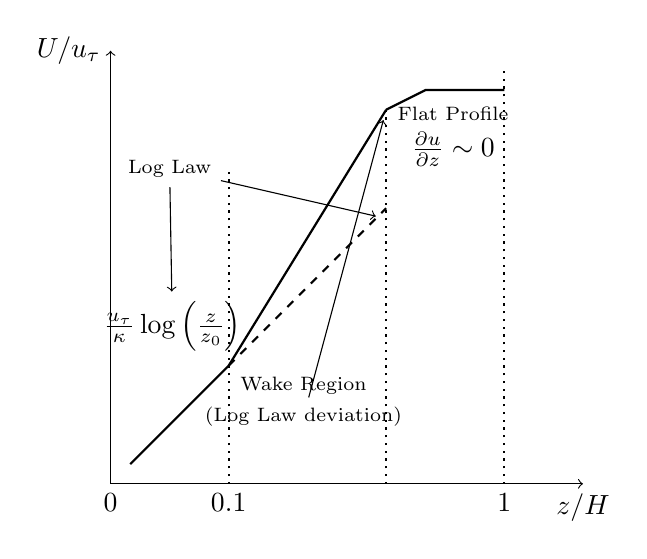
\begin{tikzpicture}[out=0,in=180,relative]

% horizontal axis
\draw[->] (0,0) -- (6,0) node[anchor=north] {\normalsize ${z}/{H}$};
% labels
\draw	(0,0) node[anchor=north] {0}
		(1.5,0) node[anchor=north] {0.1}
		(3.5,0) node[anchor=north] {}
		(5,0) node[anchor=north] {1};
% ranges
%\draw	(1,3.5) node{{\scriptsize Constant flux}}
%		(4,3.5) node{{\scriptsize Field weakening}};

% vertical axis
\draw[->] (0,0) -- (0,5.5) node[anchor=east] {\normalsize ${{U}}/{u_{\tau}}$};
% nominal speed
\draw[thick,dotted] (1.5,0) -- (1.5,4);

% Us
\draw[thick] (0.25,0.25) -- (1.5,1.5) node (a_2b) {};
\draw[thick,dashed] (1.5,1.5) -- (3.5,3.5) node[anchor=north] (a_2) {};
%\draw[->] (0.25,0.25) -- (1.5,1.5)

%\draw (1,1.5) node {$U_s$}; %label

% Us
\draw[thick] (1.5,1.5) -- (3.5,4.75);
%\draw (2,1.5) node {$U_s$}; %label
\draw[thick,dotted] (3.5,0) -- (3.5,4.75) node (a_2c) {};;

% Psis
\draw[thick] (3.5,4.75) -- (4.0,5) parabola[bend at end] (5,5);
\draw[thick,dotted] (5,0) -- (5,5.25);

\draw (0.75,4) node (a) {\scriptsize Log Law}; %label
\draw (0.785,2) node (b) {\normalsize $\frac{u_{\tau}}{\kappa}\log \left(\frac{z}{z_0}\right)$}; %label
\draw (2.45,1.25) node (c) {\scriptsize Wake Region}; %label
\draw (2.45,0.85) node (c) {\scriptsize (Log Law deviation)}; %label
\draw (4.35,4.7) node (d) {\scriptsize Flat Profile}; %label
\draw (4.35,4.25) node {\normalsize $\frac{\partial \pmb{u}}{\partial z} \sim 0$}; %label

\path[->] (a) edge (b)
              edge (a_2) ;
              
\path[->] (c) edge (a_2c);  
\end{tikzpicture}
\caption[Schematic of Log-Law of wall]{Schematic of log law of the wall over a rough wall for high Reynolds number. The $x$ axis is in log-scale. Within $z/H \lessapprox 0.1$, logarithimic trends observed: LOTW (Law of the Wall); beyond $z/H \sim 0.1$, log-law deviation: ``wake layer"; $z/H \sim O(1)$, $U(y)$ gradually becomes flatter, $\frac{dU}{dz} \approx 0$, at top lid - symmetry boundary conditions. (See ~\cite{pio2,porte1fun,meyers2} for details in LOTW)}           \label{fig:schematic}
\end{figure}
For first order statistics, velocity $U${(z)} is the temporal{ly} and horizontally averaged (homogeneous $x-y$ plane) streamwise mean velocity profile ${\langle \overline{\widetilde{u}}\rangle_{xy}}$. All the plots involving physical length scale $z$ has been normalized with the boundary layer thickness $H$. The temporal average has been taken for 10 sweeps of ``flow-through" time scale $L_x/U_{bulk}$ which is consistent with the literature ~\cite{kimmoinmoser}. We expect the streamwise mean velocity profile {at the lower $10-20 \%$ of the boundary layer ($z/H \sim 0.1-0.2$) to follow the logarithmic trend ($\Phi(z) = \kappa z/u_{\tau} dU/dz = 1$), deviate from the log-law ($\Phi(z) > 1$) beyond $x/H \sim 0.2$, popularly known as the ``wake-region" and a small flat region where the gradient gradually approaches zero due to the top symmetry boundary conditions. (See schematic in Figure~\ref{fig:schematic})} In the near-wall region, $z/H \sim 0.1$, $$\frac{{U(z)}}{u_{\tau}} = \frac{1}{\kappa}\log (\frac{z}{z_0}) = \frac{1}{\kappa}\log (\frac{z}{H}) + \frac{1}{\kappa}\log (\frac{H}{z_0}) = \frac{1}{\kappa}\log (\frac{z}{H}) + C \ ,$$ constant $C$ being a function of the roughness parameter. {From the perspective of physics, $C$ should be a function of $f(H/z_0)$, the two relevant scales of high $Re$ ABL; however with different tuning parameters $C_0, \ n$ of the SGS model, it is observed that $C \approx f(H/z_0; C_0,n)$ as is manifested also in the numerical model.}  
%The quantified effect of $C_0, \ n$ on $C$ is beyond the scope of the present paper, and is anticipated to be addressed in a separate article. 
Consequently, to understand the effect of SGS stresses on the log-law of the wall explicitly, yet decouple (atleast partially) the implicit effect of SGS stress on the mean velocity profile through $C$, metric in the form of non-dimensional mean velocity gradient $\Phi = \frac{\kappa z}{u_{\tau}} dU(z)/dz$ is more favourable since parametric constant $C$ can be eliminated with the use of derivatives.\\
 With $Re \sim 10^{10}$, eddy-viscosity in the current LES model results in $\nu_{t} (= (C_s\Delta)^2 \vert \widetilde{S} \vert) \gg \nu \approx 0$ which indicates the kinematic shear stress in an LES framework for a flat-plate type geometry can be given as
  \begin{align}
-\overline{\widetilde{u'}\widetilde{w'}} + \langle\overline{\nu_{t}} \rangle_{xy} \frac{d U}{d z} \approx \frac{\tau_{w}}{\rho}\left(1 - \frac{z}{H}\right). \label{mean}
\end{align}
Equation(~\ref{mean}) shows that the total stress is perfectly linear which has been reported in previous literature~\cite{kimmoinmoser,brass}.
From Equation~(\ref{mean}) (both RHS and LHS are {only} function{s} of $z$ due to homogeneity in the $xy$ direction), we obtain an estimate of the non-dimensional mean velocity gradient $\Phi(z)$ as 
\begin{equation}
\Phi(z) = \frac{\kappa z}{u_{\tau}}\frac{dU}{dz} = \frac{u_{\tau}\kappa z}{(C_s\Delta)^2 \langle \vert \widetilde{S} \vert)\rangle_{xy}}\left(1 - \frac{z}{H} + \frac{\overline{\widetilde{u'}\widetilde{w'}}(z)}{{u_{\tau}}^2}\right)
\end{equation}
, which can be further simplified as
\begin{equation}
\boxed{\Phi(z) = \frac{\kappa z}{C_s \Delta} \times \frac{u_{\tau} f(z)/ \langle\vert \widetilde{S} \vert)\rangle_{xy}}{C_s \Delta}} = A_1(z)\times A_2(z), \label{mean2b}
\end{equation}
with $f(z) = (1 - z/H + \overline{\widetilde{u'}\widetilde{w'}}/u_{\tau}^2)$ being a non-dimensional function of $z$ and $u_{\tau} = \sqrt{\tau_{w}/\rho}$. Also, it is important to note that the shear stress boundary condition is essentially a reflection of the log-law of the wall in its time averaged form (See Equation~(\ref{stress2})) which manifests $u_{\tau} = f(\widehat{\widetilde{u}_r})$ from the approximate stress boundary conditions.

It is quite straightforward to see the contributions of SGS stress and approximate stress boundary conditions {to} the non-dimensional mean velocity gradient $\Phi(z)$. {Close to the wall, the standard Smagorinsky damps the filter length scales retrieving log-law of rough wall $C_s\Delta \sim \kappa (z + z_0) \approx \kappa z$.} . The eddy turn over time of the near wall eddies {can be defined as} $t_{eddy} \sim f(z)/\langle\vert \widetilde{S} \vert\rangle_{xy}$ ({from now on,} we will use just $\widetilde{S}$ instead of $\langle\vert \widetilde{S} \vert\rangle_{xy}$ for brevity, statistical $x{y}$ directional homogeneity is implied). Since the near wall eddies are mostly subgrid scale and need to be modelled, it is not hard to relate  the eddy-turn over time of the near wall ``subgrid-eddies" with the so called {mixing length scale of eddies and they should correspond well with the Smagorinsky length scale $C_s \Delta$}.{It is thus important to realize that $\Phi (z)$ corresponding to the log-law, would potentially generate a value of 1 near wall, if trivially $A_1(z), \ A_2(z)$ are 1.}   

{It must be understood that, the \textbf{above conditions are ideal} from the perspective of physics just to give an example to the reader}. However, due to the smoothing effect of blending function in the wall-damped Smagorinsky model, the filter length scale close to the wall  $l_f = C_s\Delta$ may deviate from $\kappa z$ ($A_1 \neq 1)$ ; {may not be exactly $1$ in the near wall region, and it is the responsibility of the numerics to capture $u_{\tau}$ from the stress boundary conditions properly so as to alter the eddy mixing length $u_{\tau} t_{eddy}$, in an effort to make $A_1(z) \times A_2(z) = 1 $}.  

{From the perspective of physics, it is quite apparent that the standard Smagorinsky with wall damping by Mason and Thompson~\cite{mason} which retrieves log law scale near wall is potentially as consistent as its dynamic counterpart (standard/scale dependant) in the near wall regime (at least in the horizontally homogeneous problem) which are based entirely on mathematical empiricism (e.g. scale invariance or power law dependance of $C_s\Delta$) as presented in the previous literature~\cite{germano,porte1fun,bou1}.}  

{We would discuss these formulations in the later half of the section again corroborated by respective plots.
Hence, to summarize, the Results section would not only comprize of the \textit{first and second order statistics} but also \underline{some additional plots} commenting on the errors of $A_1(z)$ and $A_2(z)$ to corroborate the analytical predictions regarding the law of the wall and turbulence production as discussed in the previous paragraphs.}  .
\subsection{Cases I-IV}
To start with, we present the results of simulations $I-IV$ in Figures~\ref{fig:stata},~\ref{fig:stat21},~\ref{fig:stat22}. They involve statistics for different values of the filter cut-off wave-numbers $k_{c}$ (See Appendix~\ref{elfilt} for details)  with fixed parameters $n = 2, \ C_0 = 0.16$ for Standard Smagorinsky model using mid-point interpolation for approximate stress boundary condition (Refer to Section~\ref{nwm}). Figure~\ref{fig:stata} depicting mean velocity gradient shows a reasonable match with the standard Smagorinsky results of previous literature. It is interesting to see the region of "log-layer mismatch" corresponding to $\Phi(z) \approx 1.4$ (maximum 40 \% error near wall) in the lower $10\%$ of the ABL predicting similar trends to the results of Bou-Zeid et. al~\cite{bou1}. In fact previous standard Smagorinsky based LES results from Sullivan et. al~\cite{sull} and Chow et. al~\cite{chow} show similar trends of log-layer mismatch in the near wall region as shown in Figure~\ref{fig:sulchow}. The effect of filtering is {nearly} indistinguishable in the region $z/H \sim 0.1$, but conspicuous differences can be observed {at $z/H \gtrapprox 0.3$.}
% in the outer layer ($z/H \gtrapprox 0.5$). 
{Even though $k_c = 6$ shows quite {a} good match with the standard Smagorinsky counterpart~\cite{bou1} in the outer layer ($z/H > 0.3$), the results by $k_c = 1, 2, 4$ shows some reminiscent effect of logarithmic trends in lower $15-20 \%$ of the boundary layer~\cite{meyers2} and more prominent deviations into the ``wake region".} 

The results of second order statistics in Figures~\ref{fig:stat21},~\ref{fig:stat22} show that $k_c = 2,4$ has the best match with the standard Smagorinsky results of Porte-Ag\'{e}l et. al~\cite{porte1fun} except that the peaks of \textit{$v_{rms}$ and $uw_{rms}$}  are slightly over-predicted with respect to ~\cite{porte1fun} {but} the peak locations remain {similar}. {In general the stresses with $k_c = 6$ show significant effects of dissipation, resulting in smaller values of peaks for the Reynolds stresses compared to the other values of the filter parameter $k_c$}. For the kinematic shear stress $-uw_{rms}$, the near wall behaviour ($z/H \lessapprox 0.1$) of $k_c = 6$ is similar to standard Smagorinsky, while $k_c=2, 4$ has similitude with its scale dependant counterpart. It is important to mention that the location of the Reynolds-stress peaks are unchanged by the process of filtering ($k_c = 2, 4, 6$). 
\begin{figure}
\centering
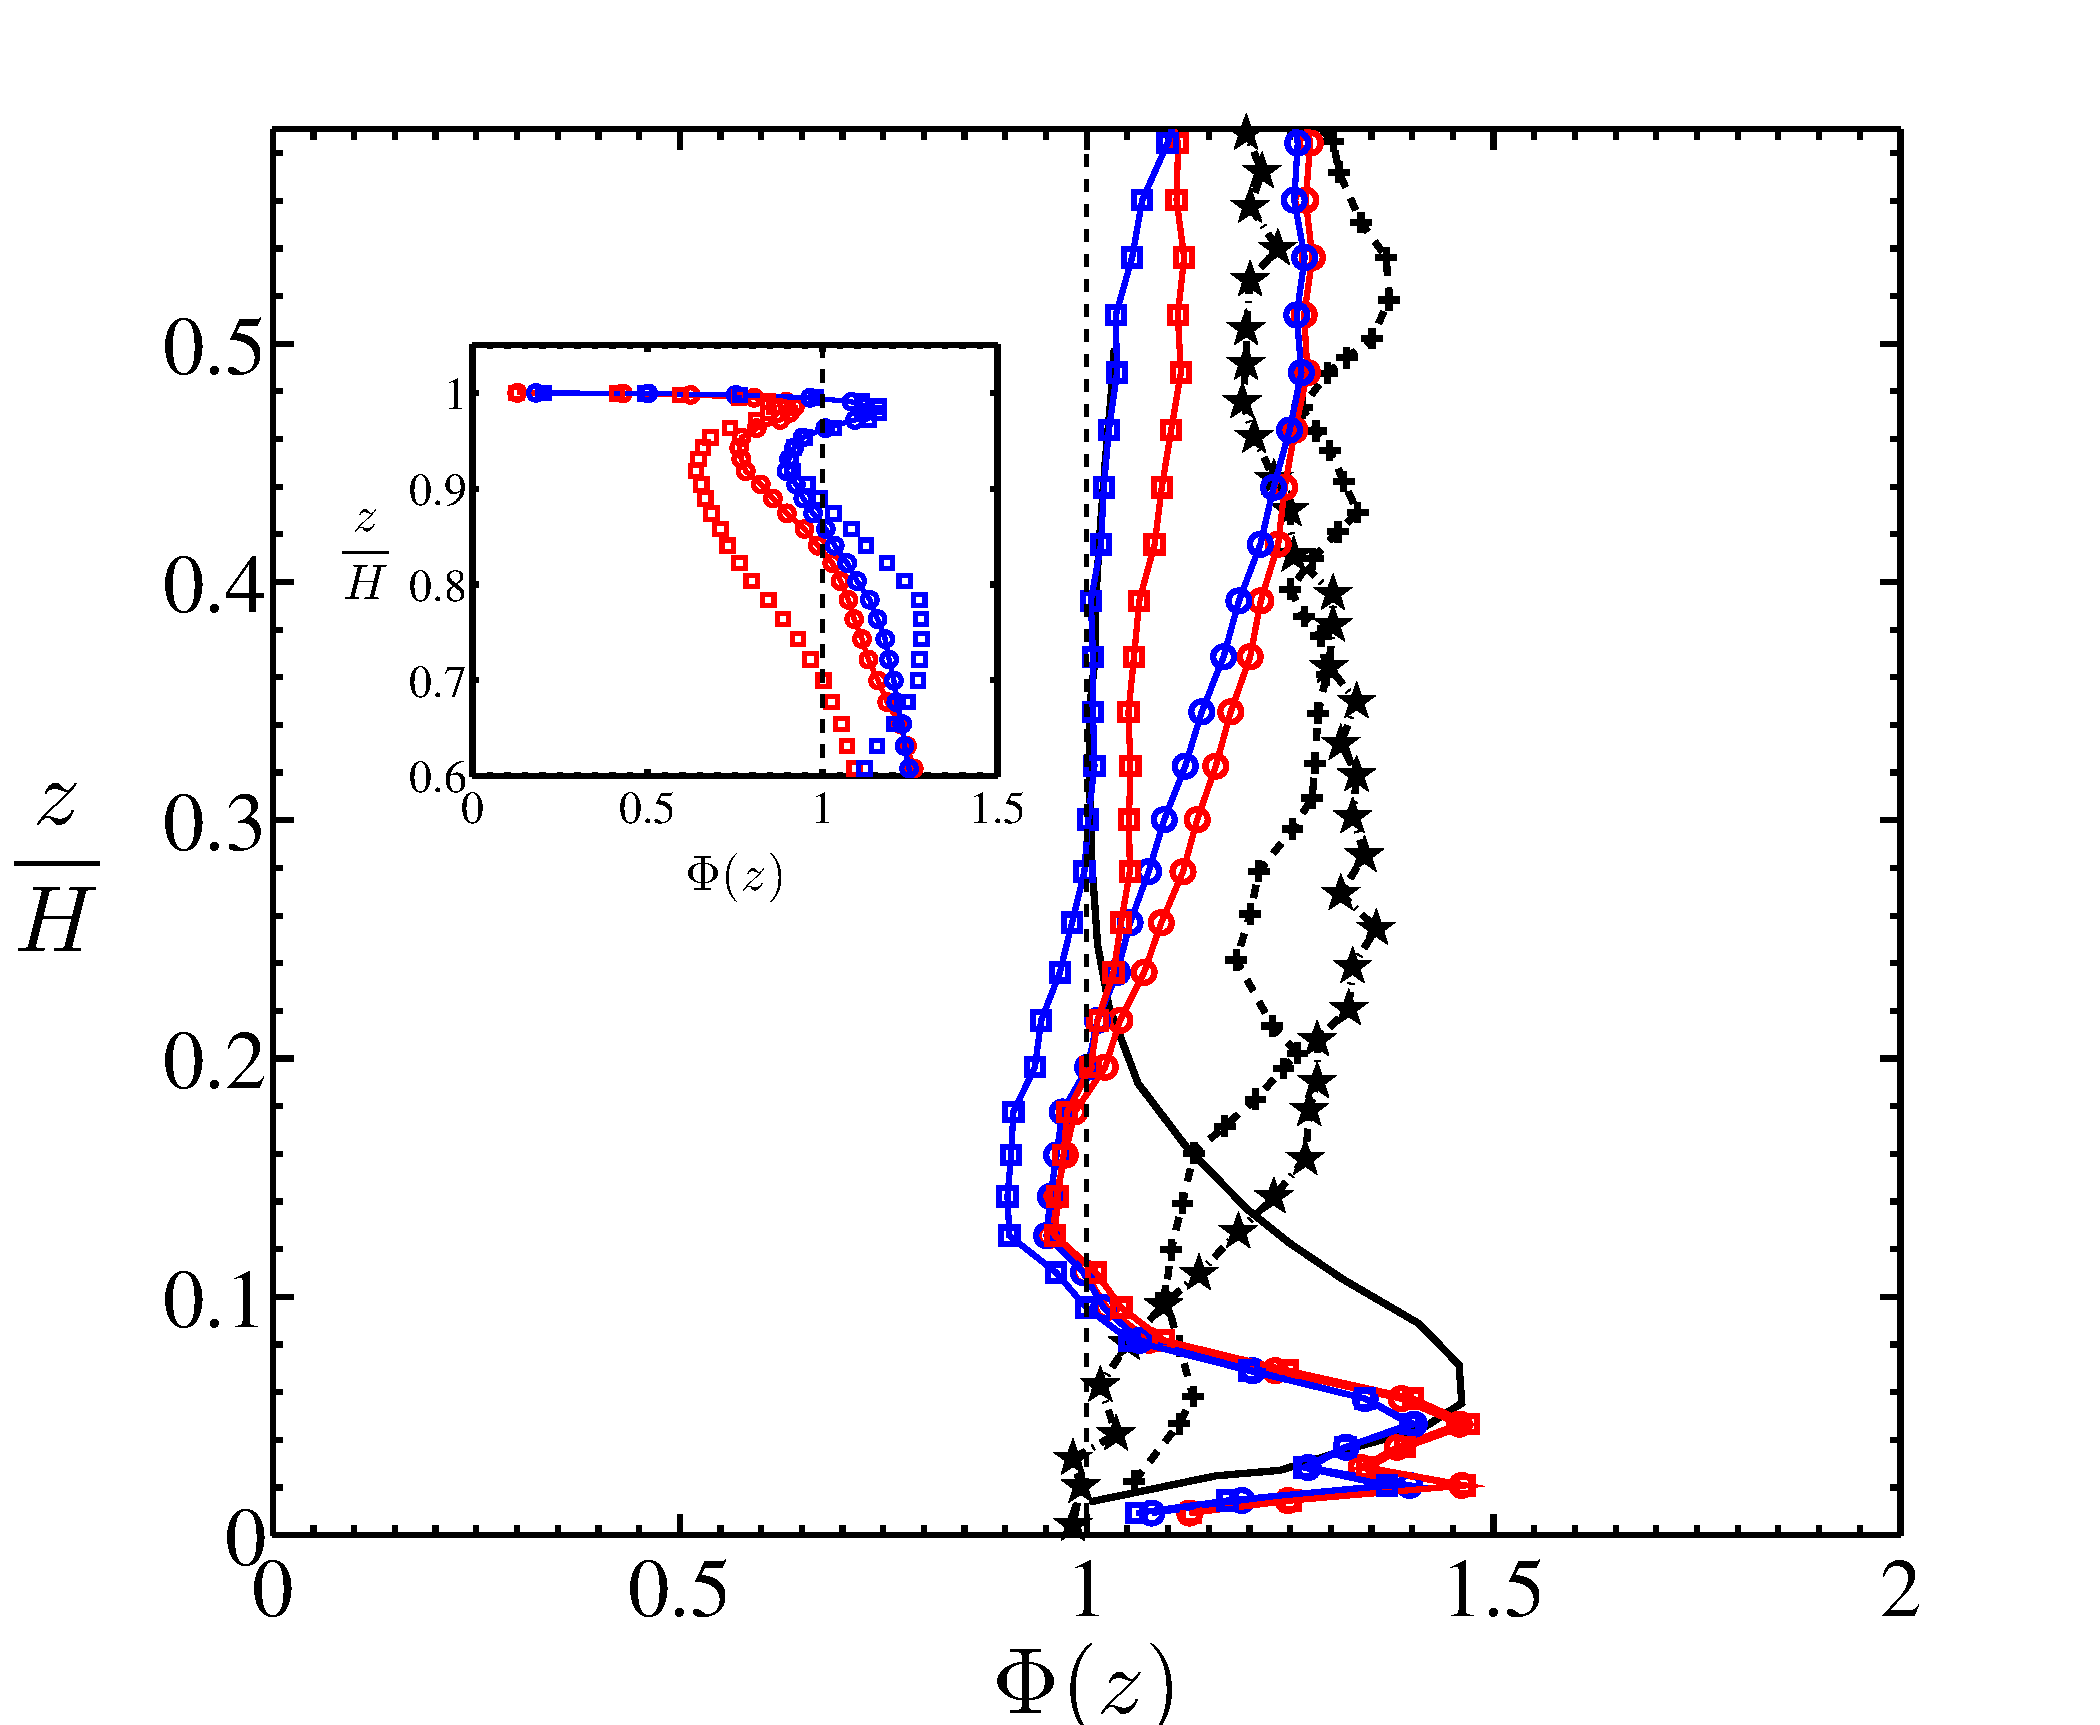
\includegraphics[width = 0.75\linewidth]{Fig3/gradient_filt_n2.pdf}        
        \caption[$\Phi(z)$, Case $I-IV$]{Non dimensinonal mean streamwise velocity gradient $\phi(z)$ vs $z/H$. Red, Blue curves: current simulations $I-IV$ ($n = 2, \ C_0 = 0.16$); Black curves from the literature~\cite{porte1fun,bou1}. Red $\Box$, $k_{c}=1$; $\circ$, $k_{c}=2$; Blue $\circ$, $k_{c} = 4$; Blue $\Box$, $k_{c} = 6$. Black $+$ scale dependant dynamic Smagorinsky for Port$\acute{e}$-Agel et al.~\cite{porte1fun}; $-$ , standard Smagorinsky, Bou-Zeid et. al, $\star$, Lagrangian scale dependant dynamic Smagorinsky with filtering, Bou-Zeid et. al~\cite{bou1}.}\label{fig:stata}
\end{figure}

\begin{figure}
\centering
        \begin{subfigure}[t]{0.42\textwidth}
                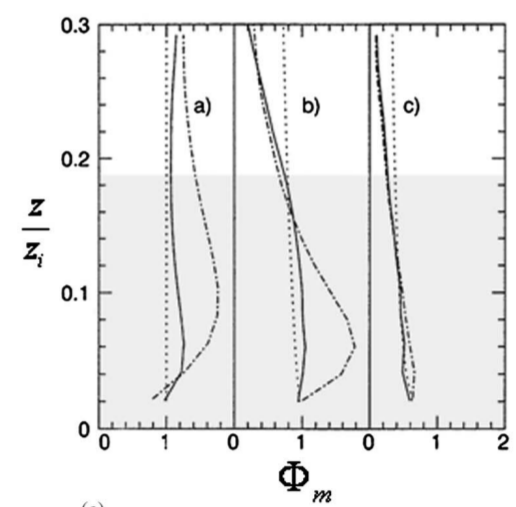
\includegraphics[width=\linewidth]{Figure/sullivan.png}
                \caption{}
                \label{fig:phi1}
        \end{subfigure}%
        \centering
        \begin{subfigure}[t]{0.475\textwidth}
                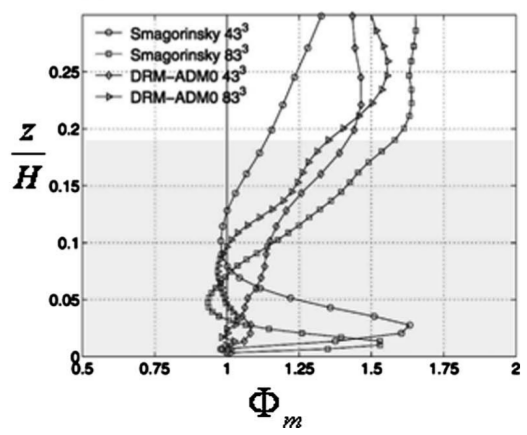
\includegraphics[width=\linewidth]{Figure/chow.png}
                \caption{}
                \label{fig:phi2}
        \end{subfigure}%
        \caption[Law of Wall: Previous studies]{Non dimensinonal mean streamwise velocity gradient $\phi(z)$ vs boundary layer height in previous LES studies (standard Smagorinsky). (a) Sullivan et. al~\cite{sull}; $z_i$ is the conventional ABL depth used {in the} atmospheric community as the height where vertical turbulent heat flux is a minimum. (b) Chow et. al~\cite{chow} uses similar simulations as in the current results without capping inversion. The plots are taken from Brasseur and Wei~\cite{brass}}\label{fig:sulchow}
\end{figure}
\begin{figure}
\centering
        \begin{subfigure}[t]{0.75\textwidth}
                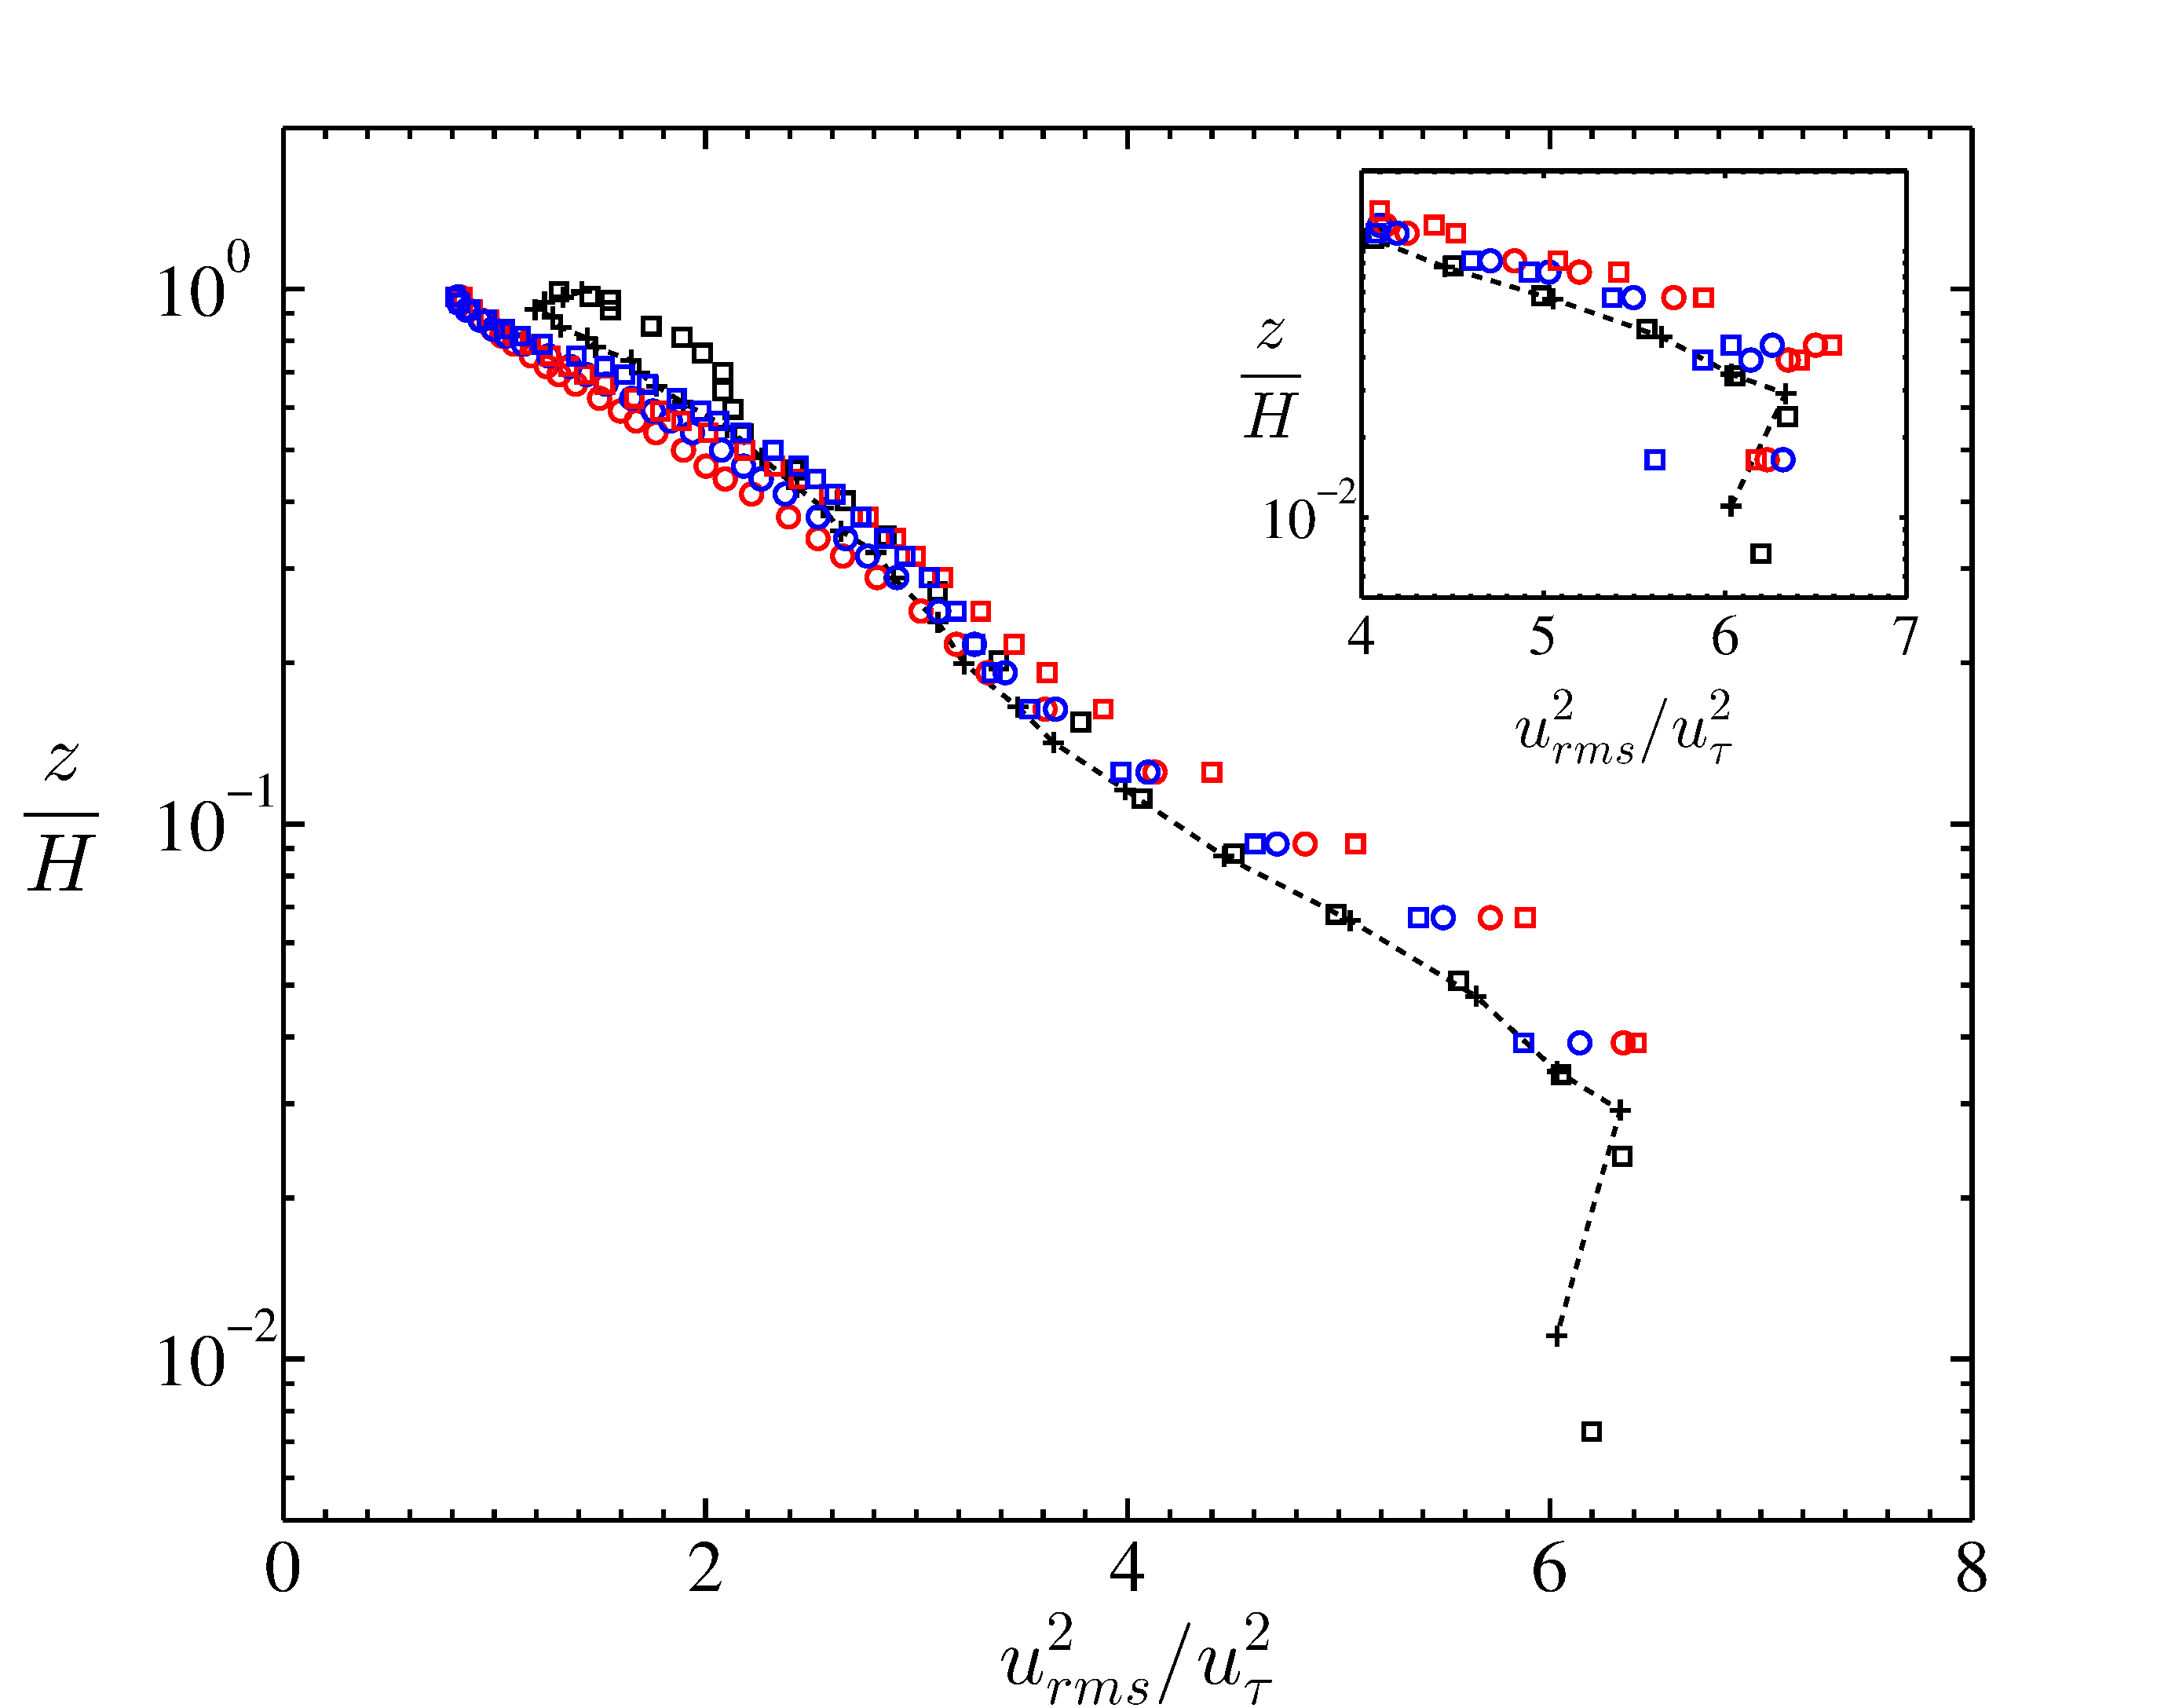
\includegraphics[width=\linewidth]{Fig3/urms_filter_n2.pdf}
                \caption{}
                \label{fig:urms}
        \end{subfigure}
        \centering
        \begin{subfigure}[t]{0.75\textwidth}
                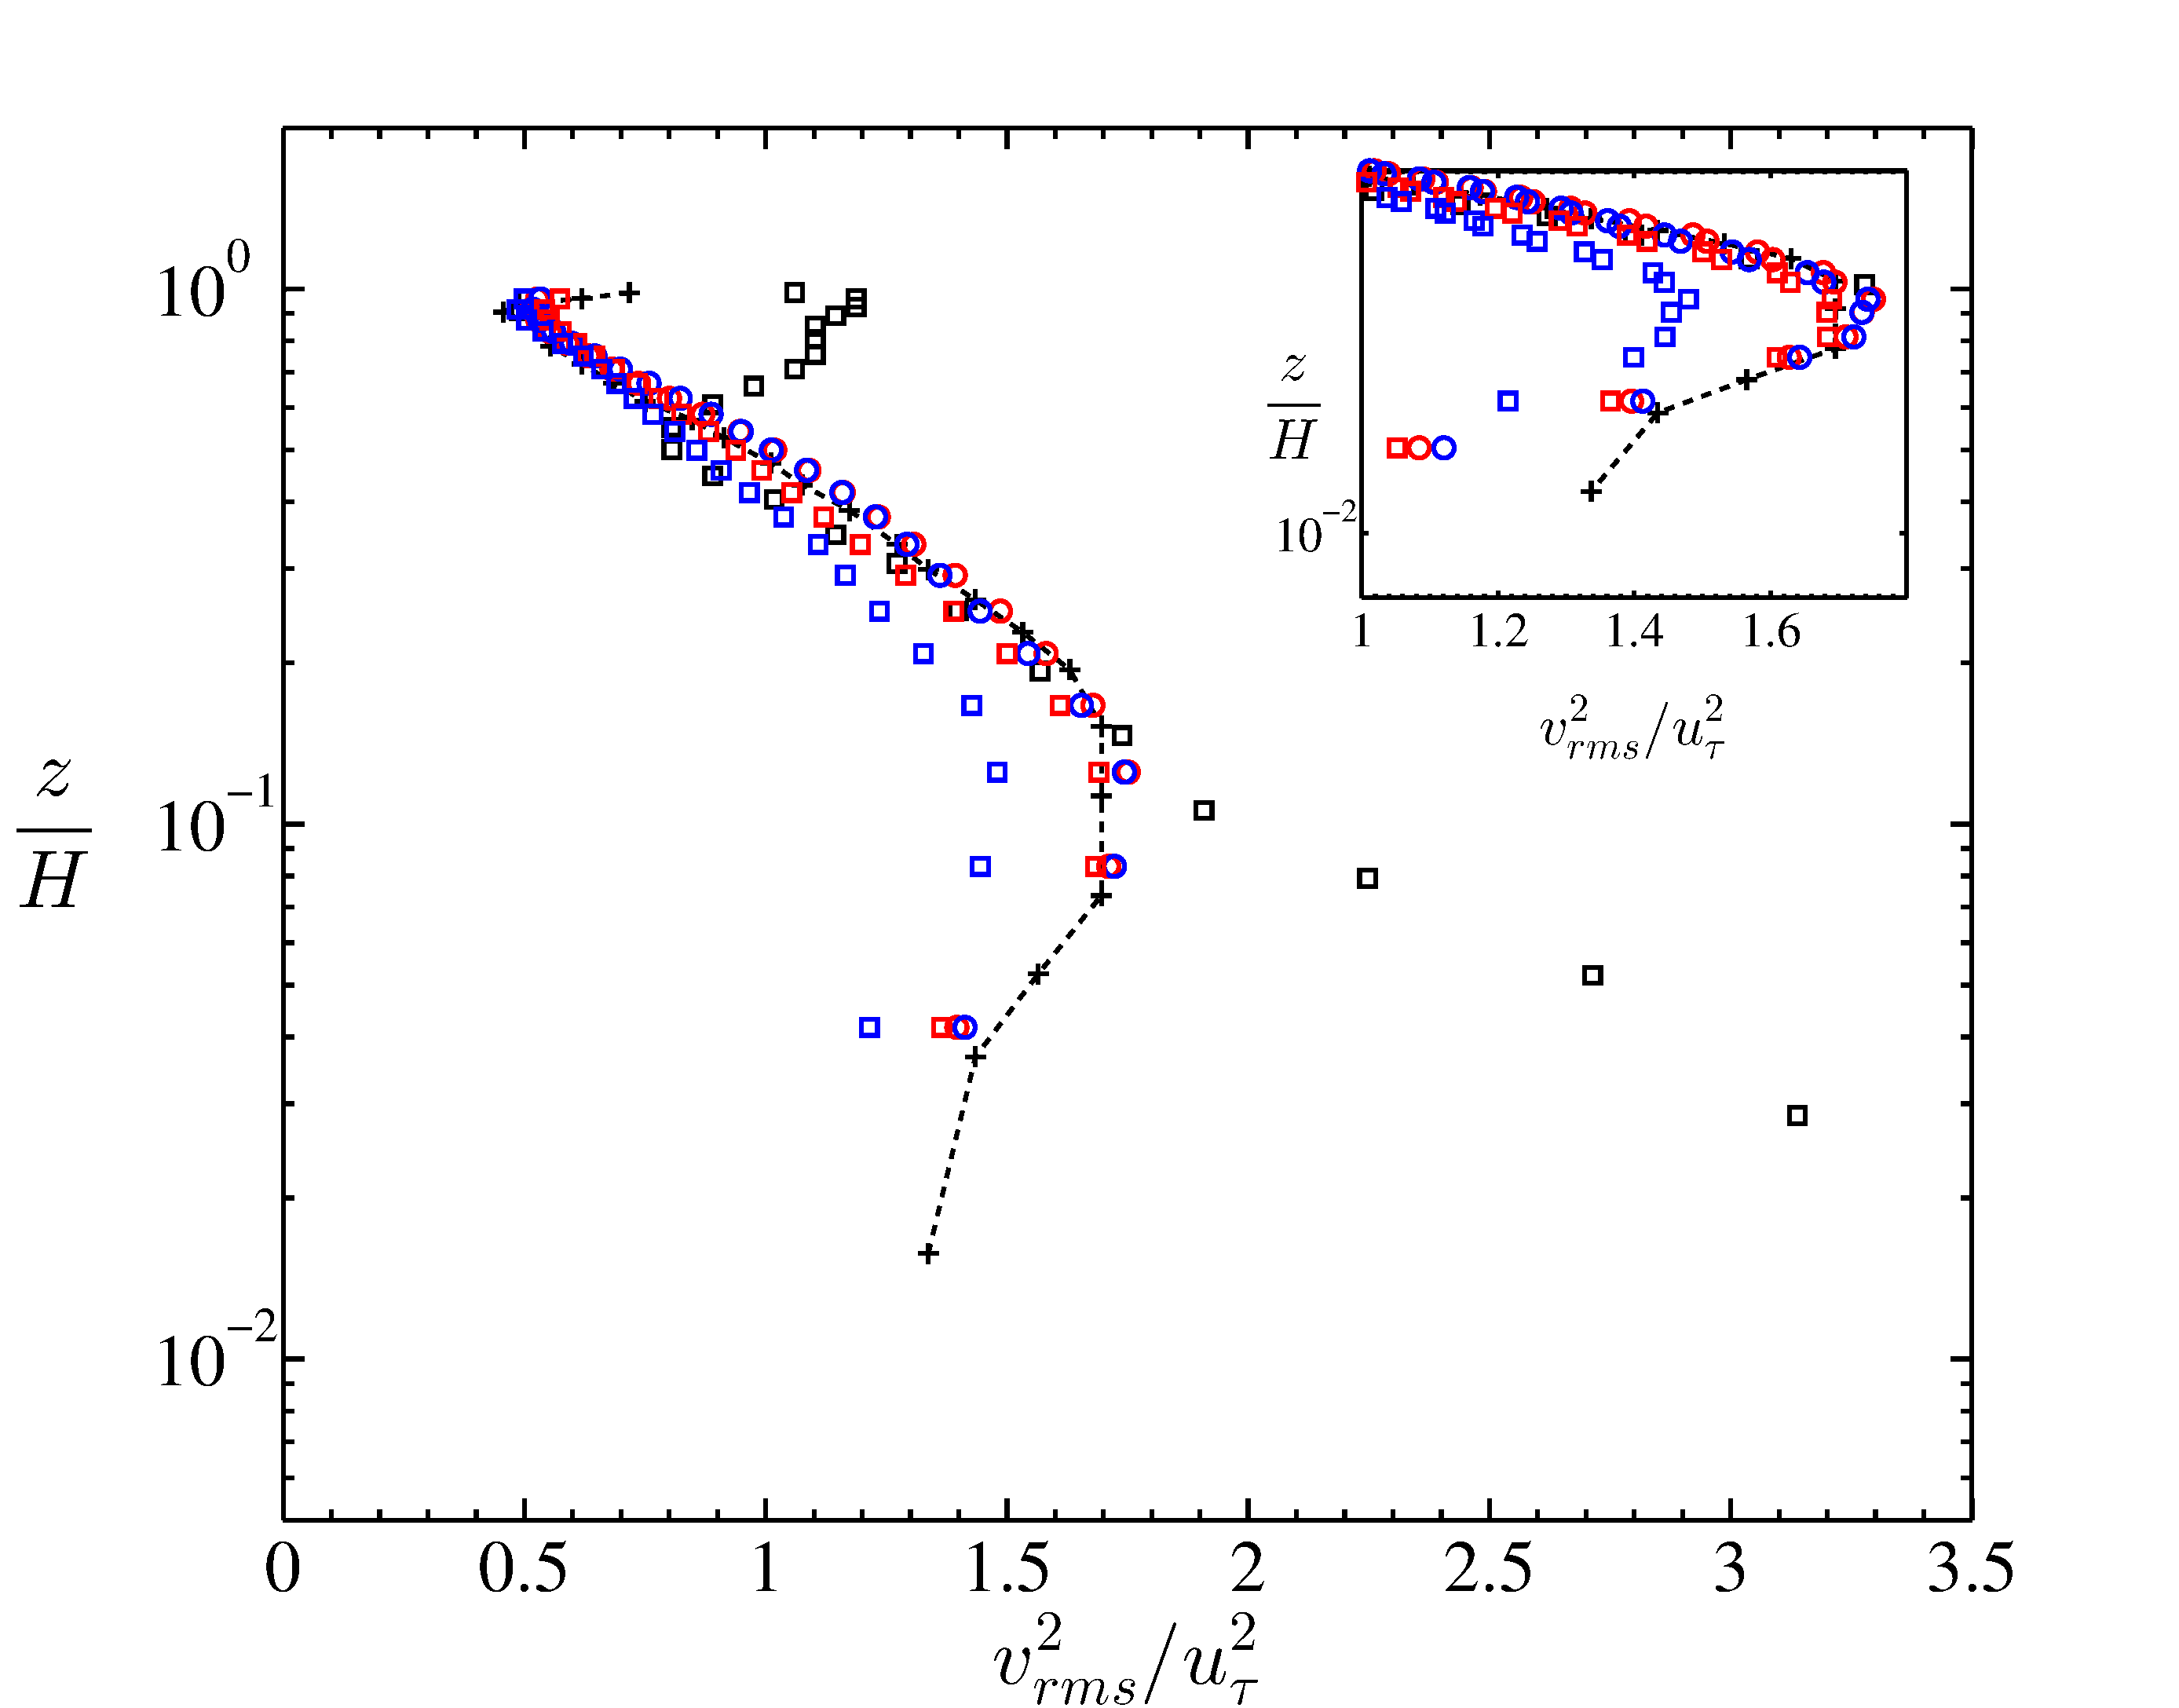
\includegraphics[width=\linewidth]{Fig3/vrms_filter_n2.pdf}
                \caption{}
                \label{fig:vrms}
        \end{subfigure}
        \caption[Second order statistics $u_{rms}, \ v_{rms}$, Case $I-IV$]{Second order statistics for ABL simulations: Case $I-IV$. (a) $u_{rms}$ (b) $v_{rms}$. Red, Blue curves: current simulations $I-IV$ ($n = 2, \ C_0 = 0.16$);  Red $\Box$, $k_{c}=1$; $\circ$, $k_{c}=2$; Blue $\circ$, $k_{c} = 4$; Blue $\Box$, $k_{c} = 6$.  Black $-+$, standard Smagorinsky ($C_s = 0.10, n = 2$) {for Port$\acute{e}$-Agel et al.~\cite{porte1fun}} and black $\Box$ scale dependant dynamic Smagorinsky for Port$\acute{e}$-Agel et al.~\cite{porte1fun}}\label{fig:stat21}
\end{figure}
\begin{figure}        
        \centering
        \begin{subfigure}[t]{0.75\textwidth}
                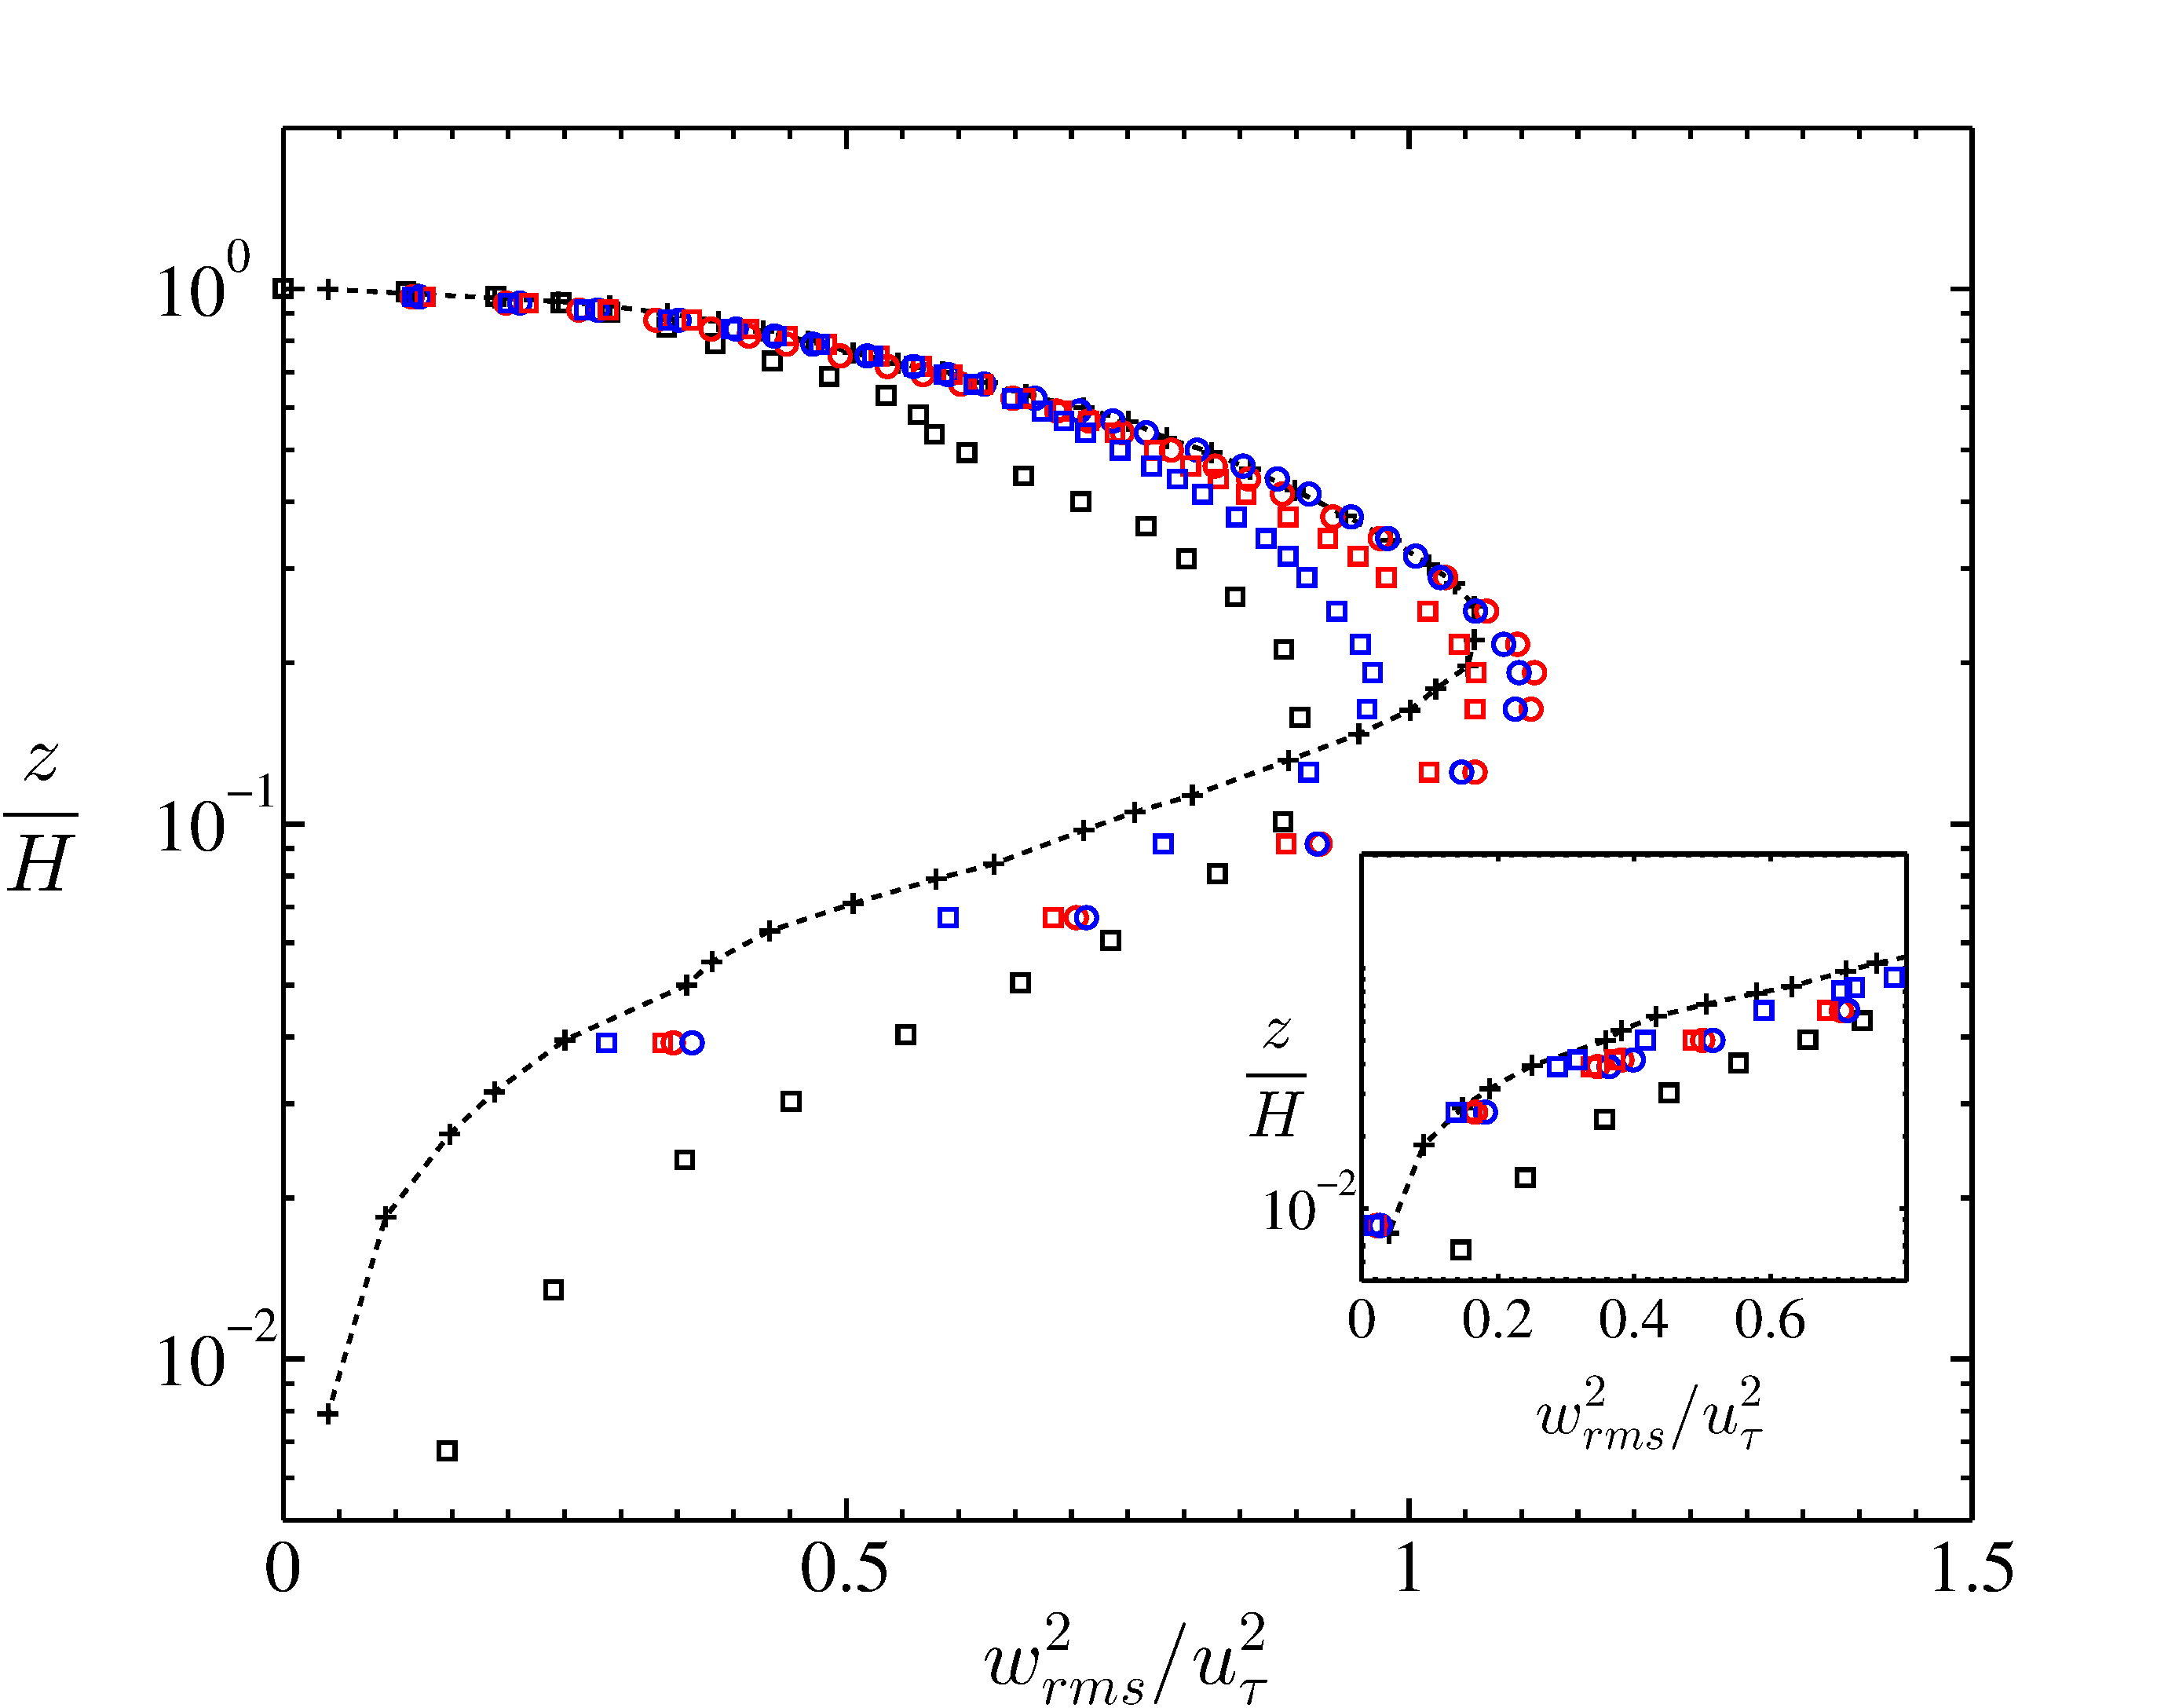
\includegraphics[width=\linewidth]{Fig3/wrms_filter_n2.pdf}
                \caption{}
                \label{fig:wrms}
        \end{subfigure}
        \centering
        \begin{subfigure}[t]{0.75\textwidth}
                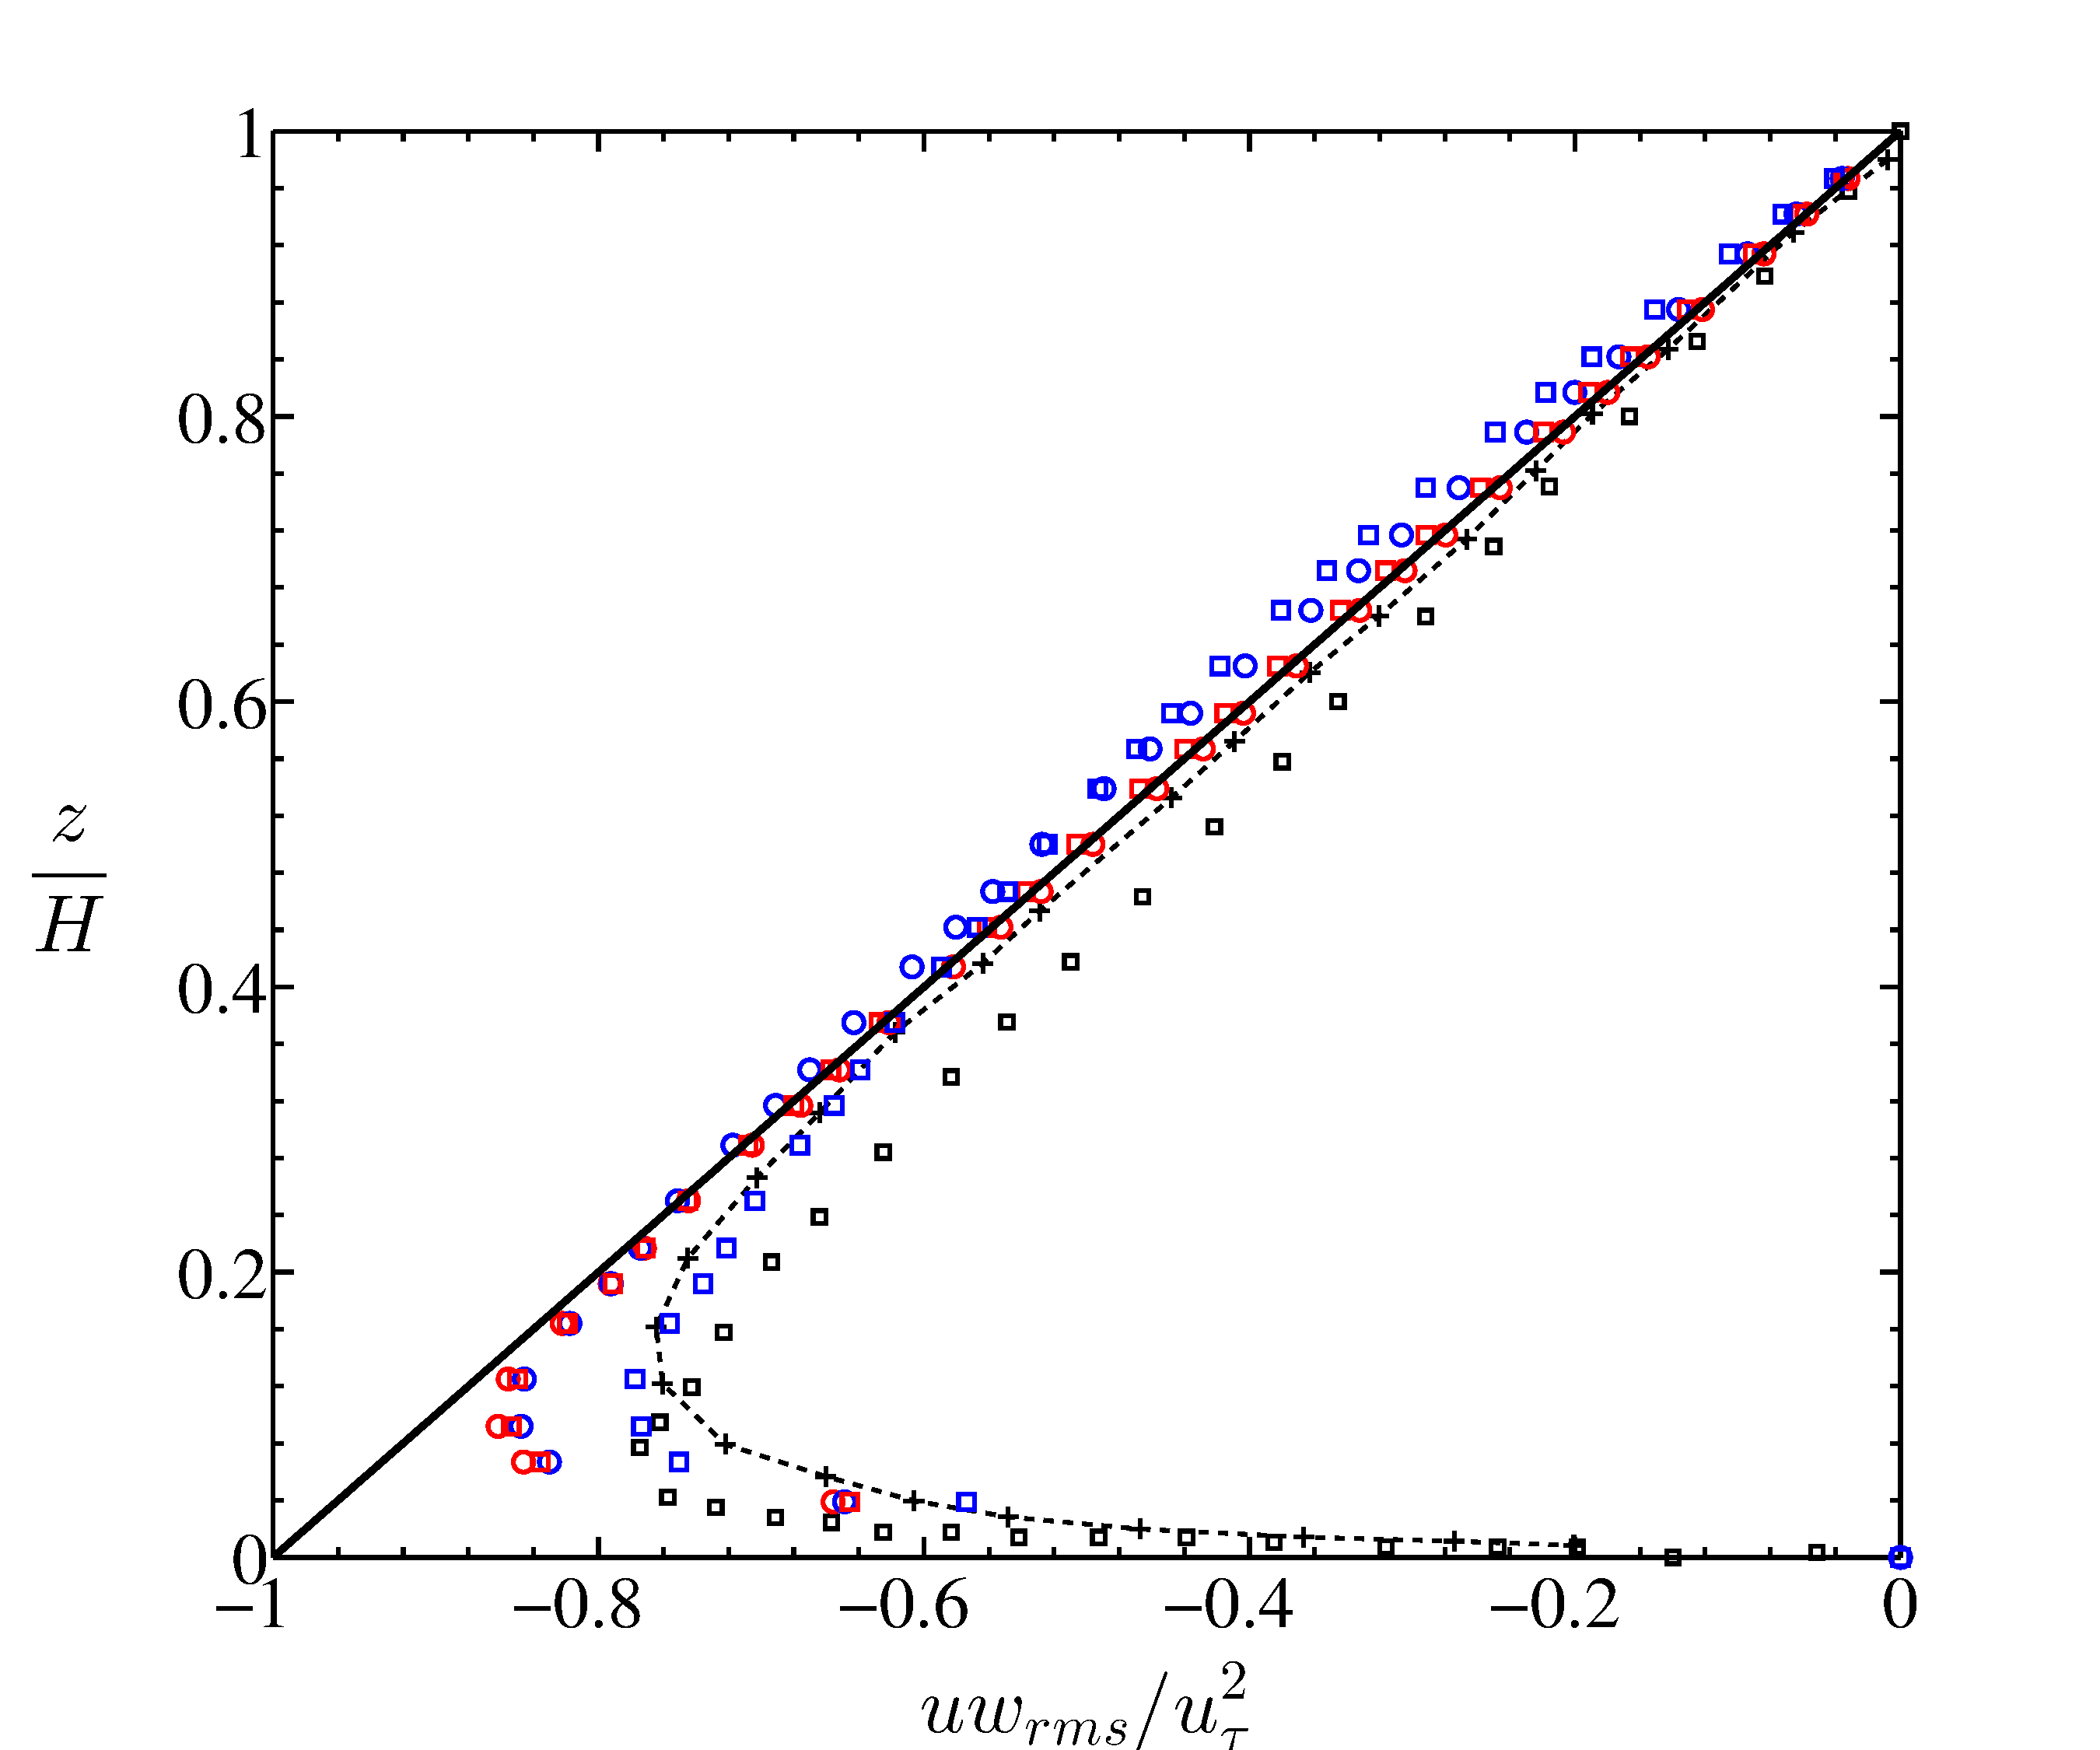
\includegraphics[width=\linewidth]{Fig3/uwrms_filter_n2.pdf}
                \caption{}
                \label{fig:uwrms}
        \end{subfigure}
        \caption[Second order statistics $w_{rms}, \ uw_{rms}$, Case $I-IV$]{Second order statistics for ABL simulations: Case $I-IV$. (a) $w_{rms}$ (b) $uw_{rms}$. Red, Blue curves: current simulations $I-IV$ ($n = 2, \ C_0 = 0.16$);  Red $\Box$, $k_{c}=1$; $\circ$, $k_{c}=2$; Blue $\circ$, $k_{c} = 4$; Blue $\Box$, $k_{c} = 6$.  Black $-+$, standard Smagorinsky ($C_s = 0.10, n = 2$) and black $\Box$ scale dependant dynamic Smagorinsky for Port$\acute{e}$-Agel et al.~\cite{porte1fun}. Solid black line in (b) is the ideal linear trend of non-dimensional total stress.}\label{fig:stat22}
\end{figure}
\subsection{Cases V-VII}
This section describes the statistics involved with tuning parameters $C_0 = 0.17, n = 1$.  The non-dimensional velocity gradient in Figure~\ref{fig:statba} shows similar trends with Chow et. al~\cite{chow} as was observed in Cases I-IV. The log-layer mismatch with $k_c = 2$ is slightly higher ($\sim 60\%$) compared to the mismatch with $k_c = 4, 6$ ($\sim 40-50\%$) and the peak is closer towards the wall compared to the cases I-IV. The plot with $k_c = 6$ shows some reminiscent logarithmic trends {in the first $15-20\%$} of the ABL and yet displays some prominence in the wake region ($\phi(z) > 1$), compared to $k_c = 2, 4$. All the plots with different $k_c$ show a relatively slower decay to the ``flat-profile" region compared to the plots with $n=2$ (Cases I - IV).\\
The results of second order statistics are shown in Figure{s}~\ref{fig:stat021a},~\ref{fig:stat022a}. The plots with $k_c = 4, 6$ show excellent match with the standard Smagorinsky model in the outer layer of the flow~\cite{porte1fun}. The discrepancies in the inner layer compared to the Cases I-IV can be manifested in the 
{smaller values}  of resolved ``stresses" (especially $v_{rms}$, $w_{rms}$, $uw_{rms}$) with $k_c = 4$ instead of $k_c = 6$ as observed in Cases I-IV. To summarize, 
%even 
with $n = 1, C_0 = 0.17$, the phenomenon of ``logarithmic mismatch" can {still} be seen as in Case I-IV. 
\begin{figure}
\centering
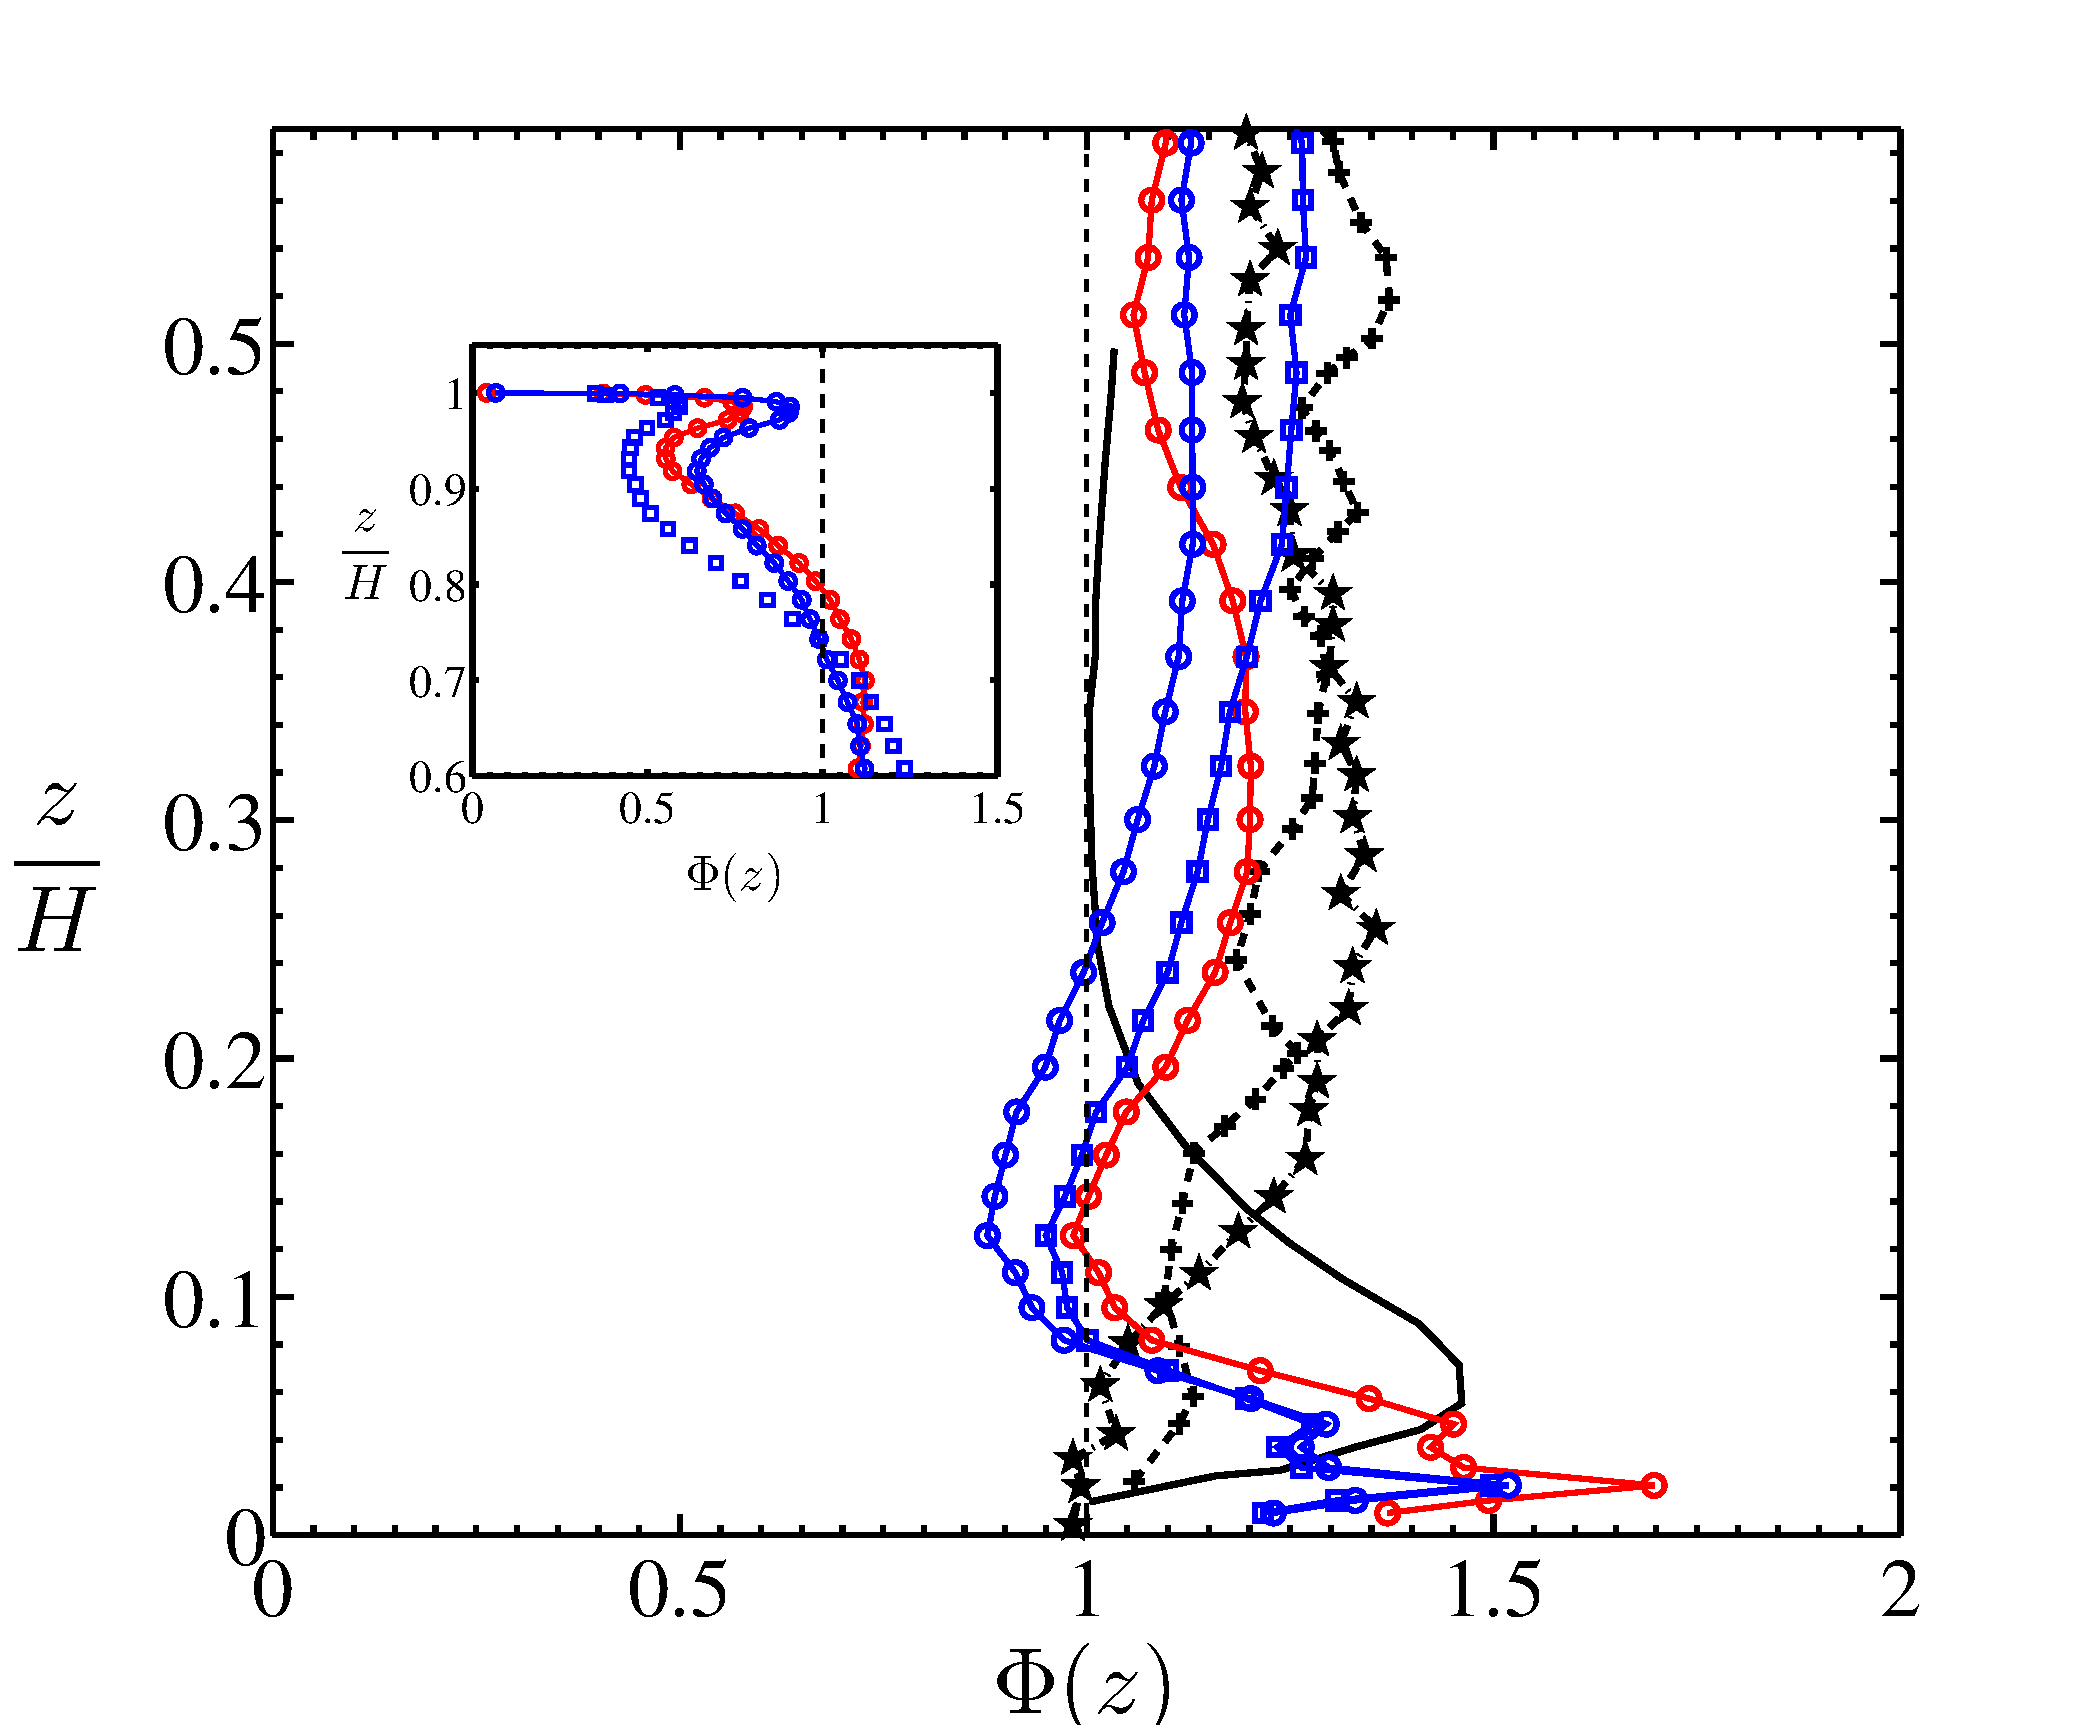
\includegraphics[width = 0.75\linewidth]{Fig3/gradient_filt_n1.pdf}        
        \caption[$\Phi(z)$, Case $V-VII$]{Non dimensinonal mean streamwise velocity gradient $\phi(z)$ vs $z/H$. Red, Blue curves: current simulations $V-VII$ ($n = 1, \ C_0 = 0.17$); Black curves from the literature~\cite{porte1fun,bou1}. Red $\circ$, $k_{c}=2$; Blue $\circ$, $k_{c} = 4$; Blue $\Box$, $k_{c} = 6$. Black $+$ scale dependant dynamic Smagorinsky for Port$\acute{e}$-Agel et al.~\cite{porte1fun}; $-$ , standard Smagorinsky, $\star$, Lagrangian scale dependant dynamic Smagorinsky with filtering, Bou-Zeid et. al~\cite{bou1}}\label{fig:statba}
\end{figure}

\begin{figure}
\centering
        \begin{subfigure}[t]{0.75\textwidth}
                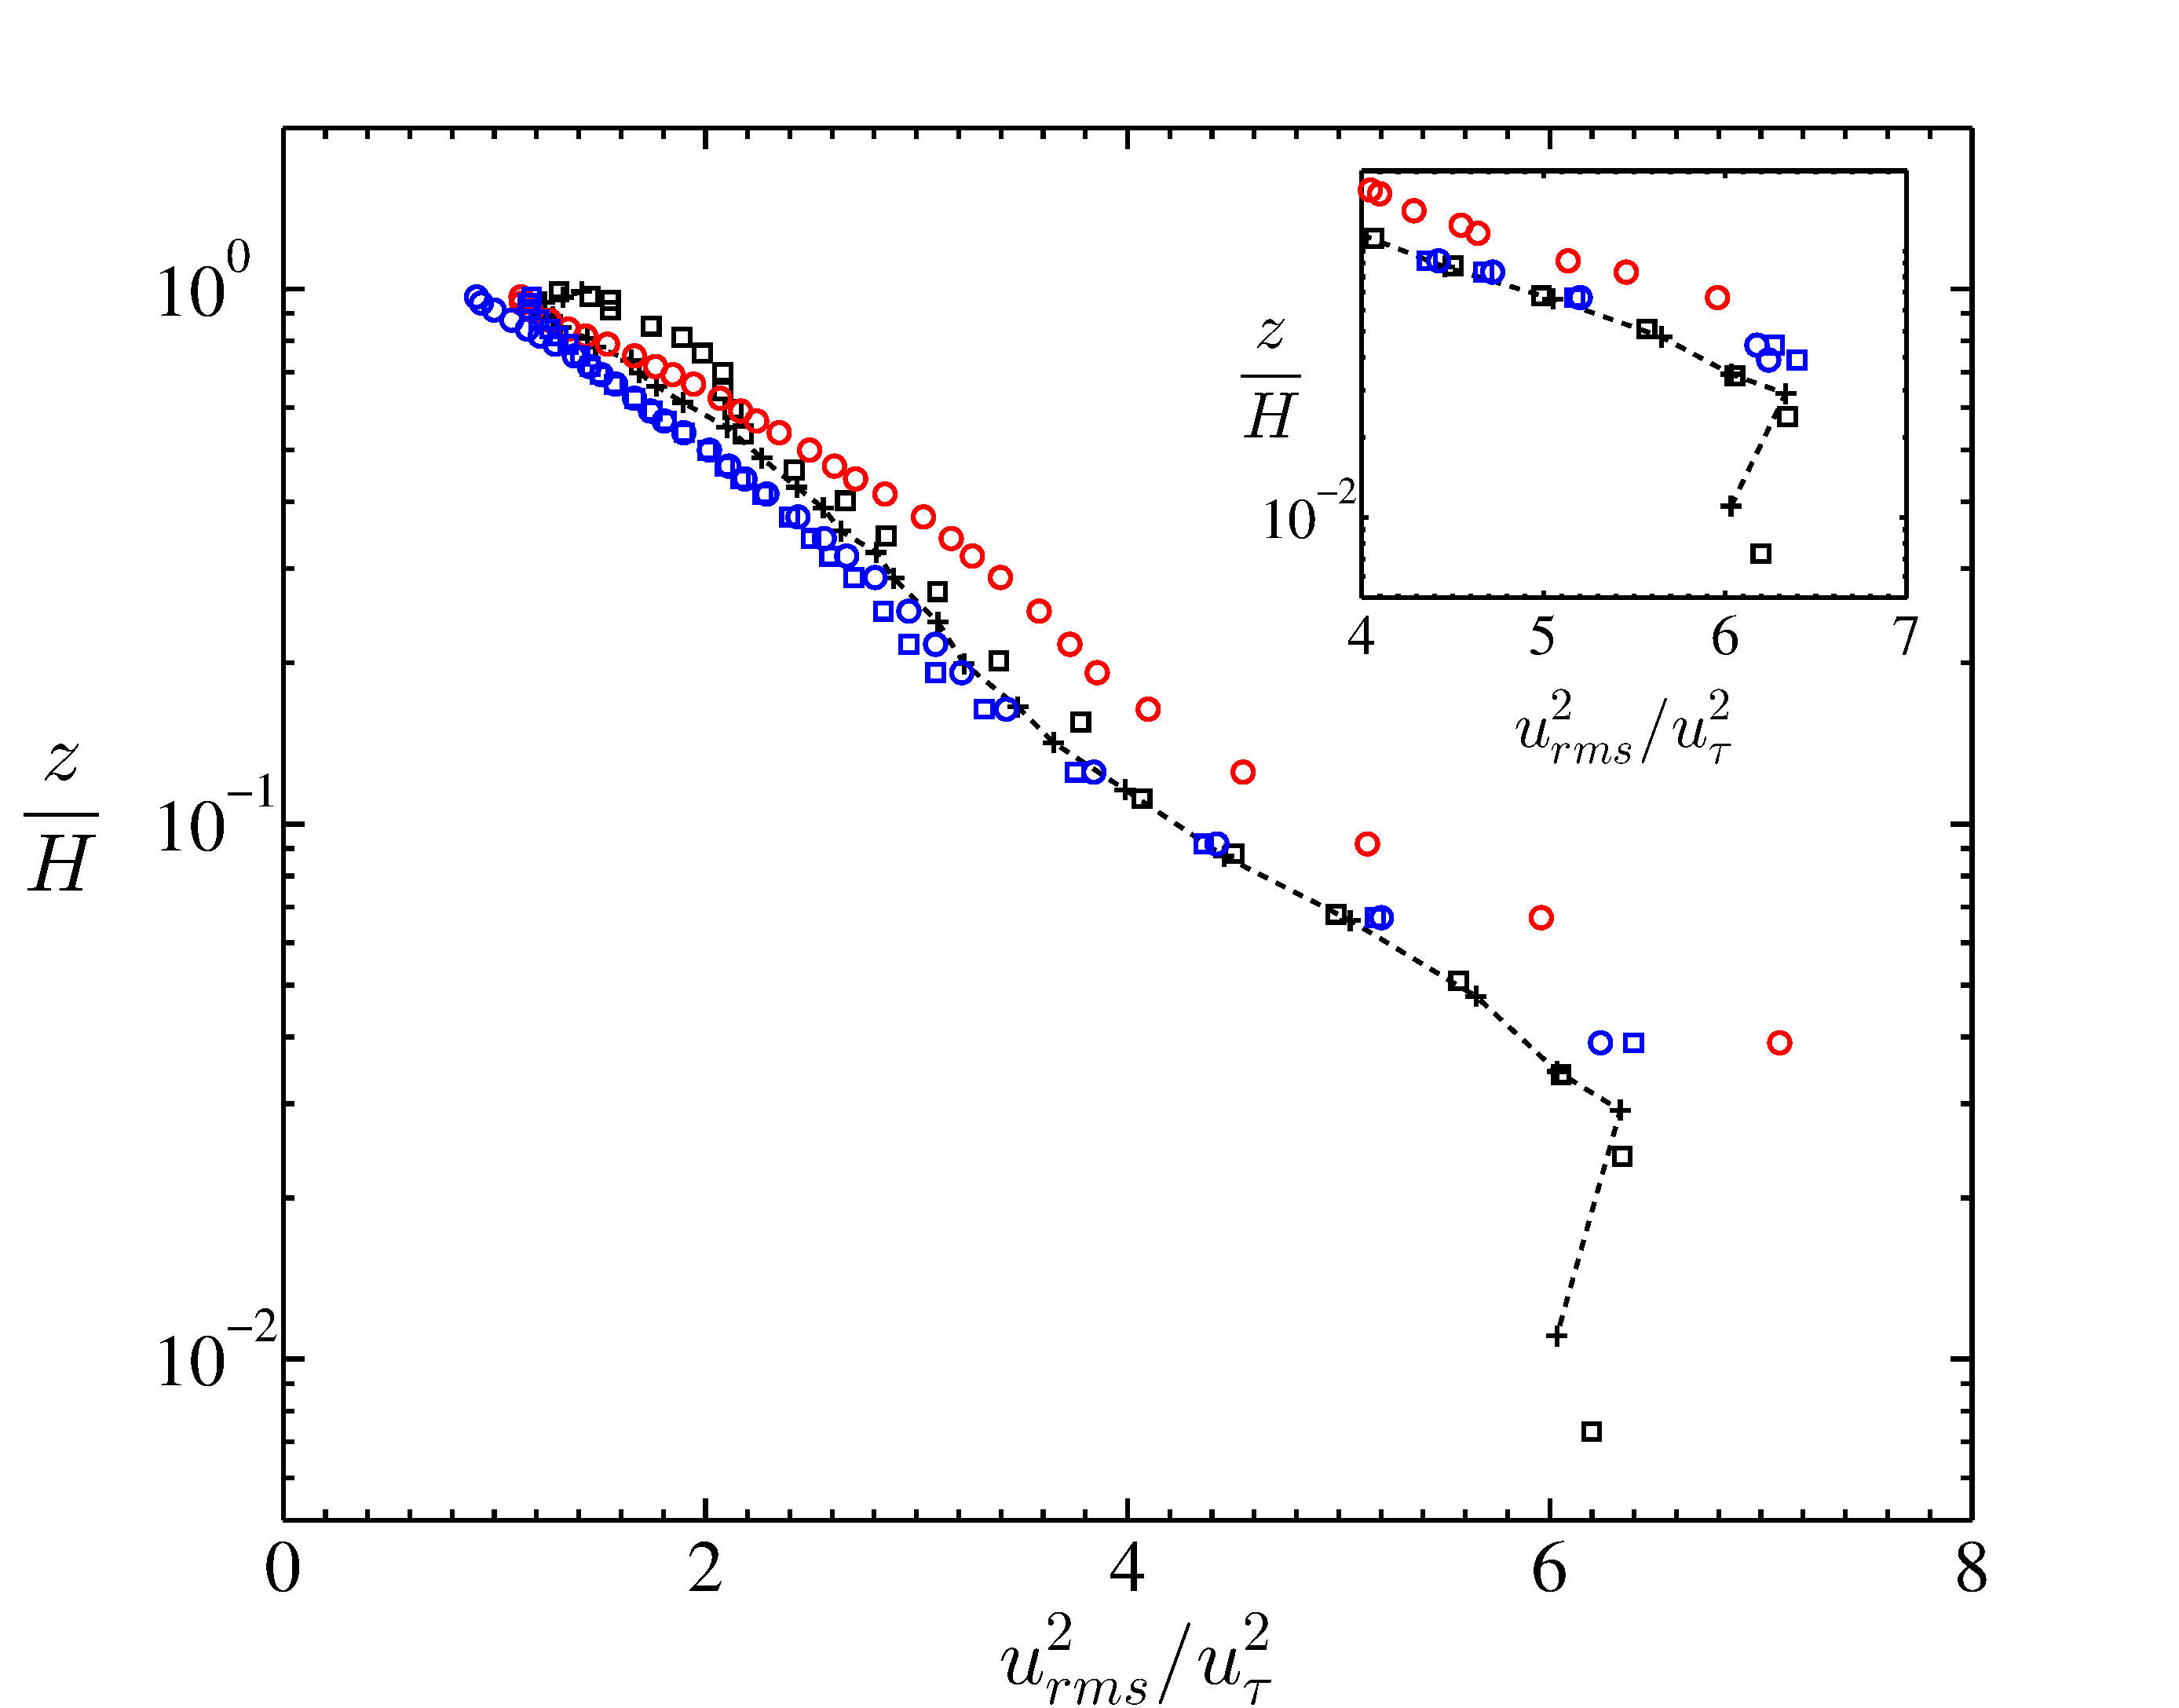
\includegraphics[width=\linewidth]{Fig3/urms_filter_n1.pdf}
                \caption{}
                \label{fig:urms1a}
        \end{subfigure}
        \centering
        \begin{subfigure}[t]{0.75\textwidth}
                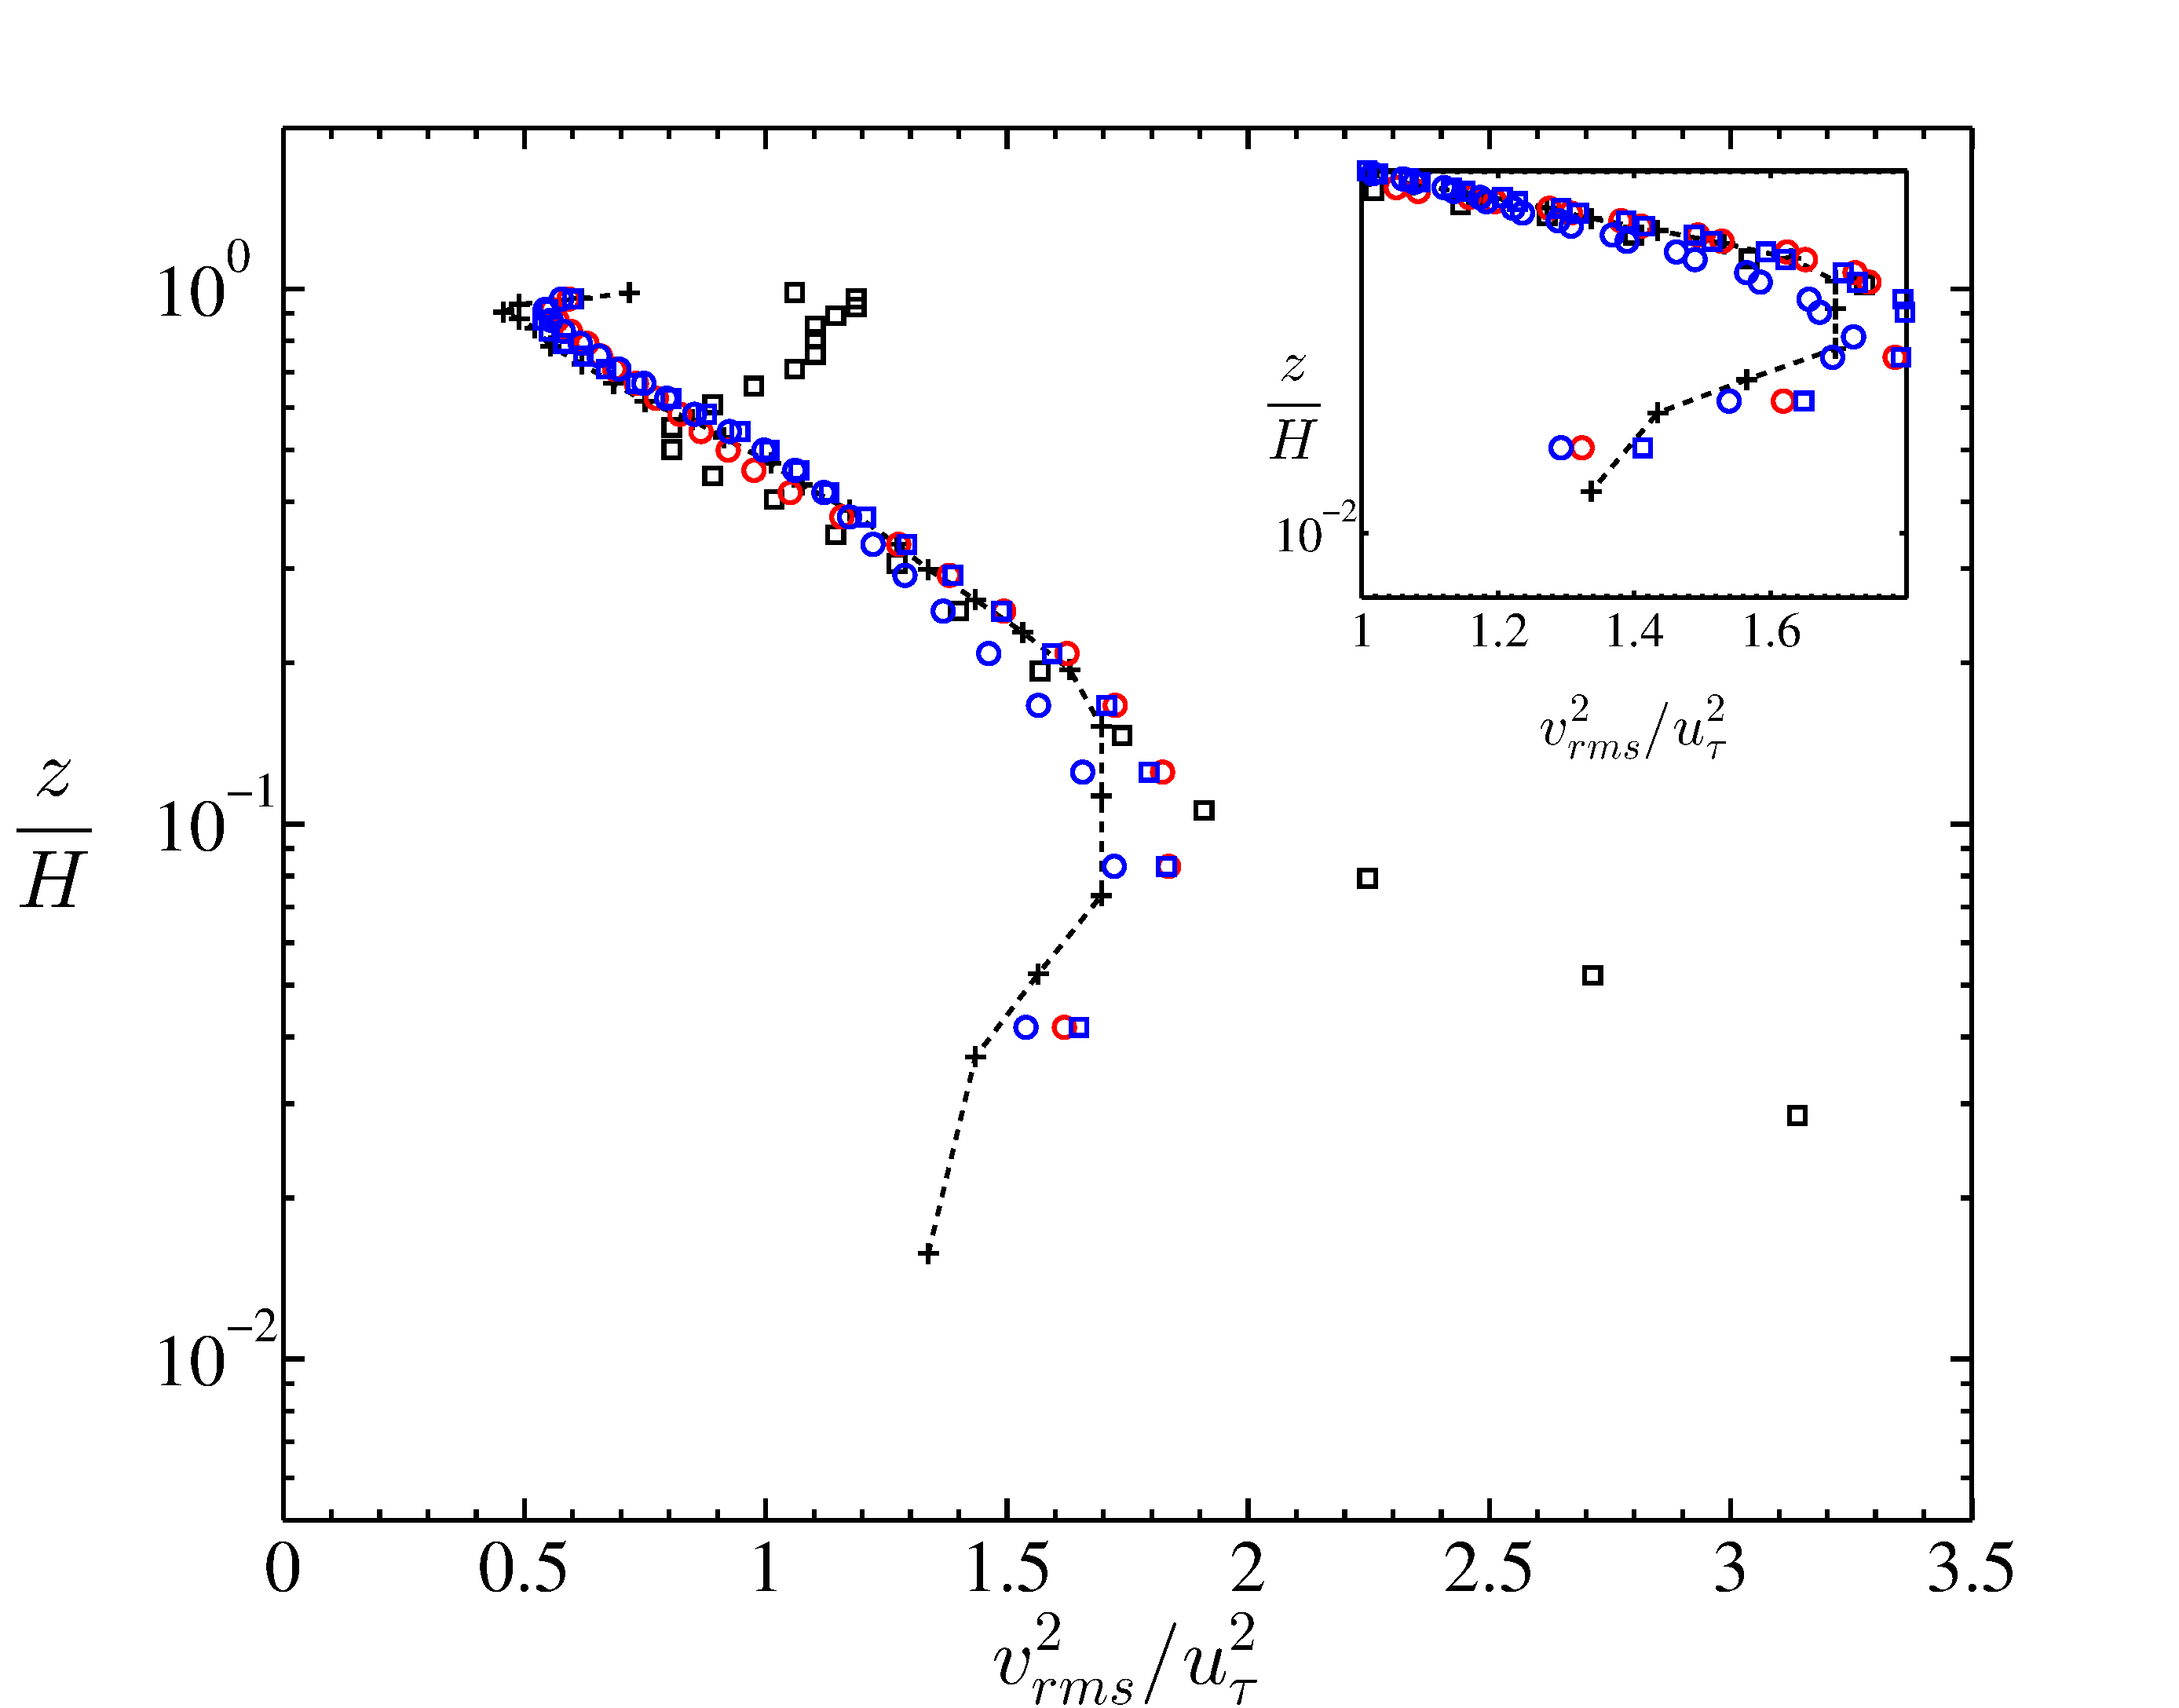
\includegraphics[width=\linewidth]{Fig3/vrms_filter_n1.pdf}
                \caption{}
                \label{fig:vrms1a}
        \end{subfigure}
        \caption[Second order statistics $u_{rms}, \ v_{rms}$, Case $V-VII$]{Second order statistics for ABL simulations: Case $V-VII$ . (a) $u_{rms}$ (b) $v_{rms}$ . Red, Blue curves: current simulations $V-VII$ ($n = 1, \ C_0 = 0.17$);  Red $\circ$, $k_{c}=2$; Blue $\circ$, $k_{c} = 4$; Blue $\Box$, $k_{c} = 6$.  Black $-+$, standard Smagorinsky ($C_s = 0.10, n = 2$) {for Port$\acute{e}$-Agel et al.~\cite{porte1fun}} and black $\Box$ scale dependant dynamic Smagorinsky for Port$\acute{e}$-Agel et al.~\cite{porte1fun}. }\label{fig:stat021a}
\end{figure}
\begin{figure}
        \centering
        \begin{subfigure}[t]{0.75\textwidth}
                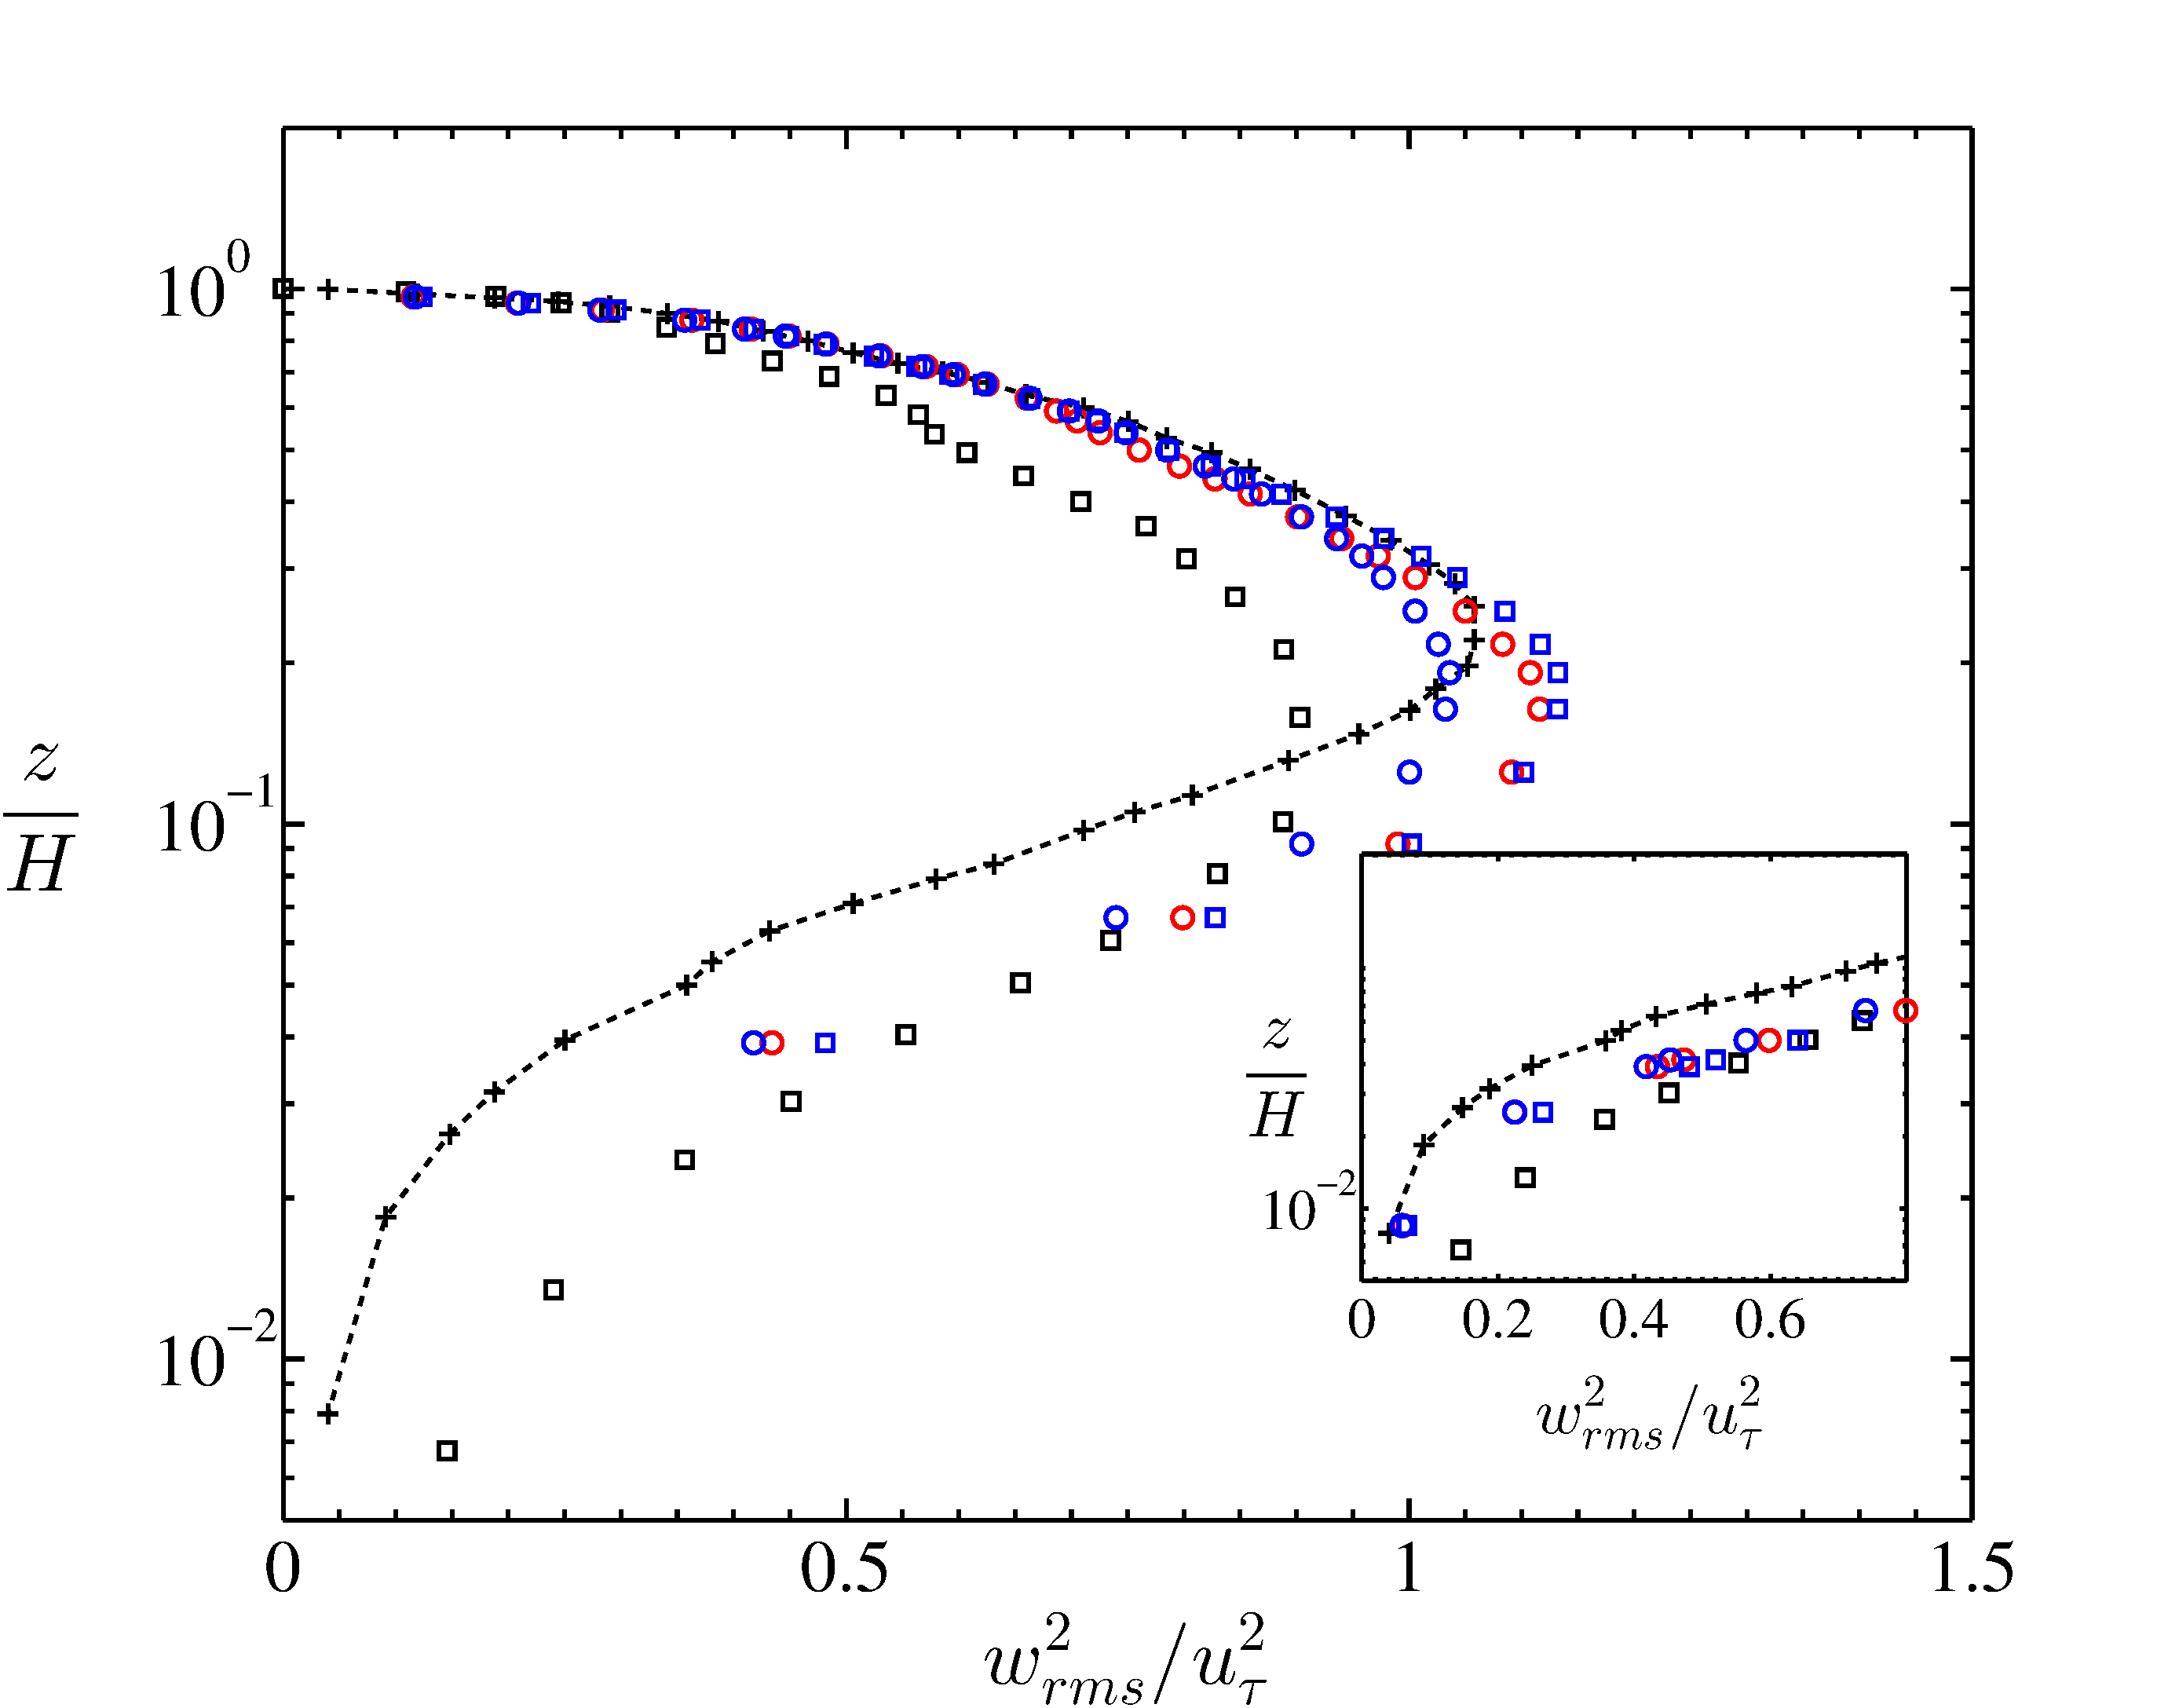
\includegraphics[width=\linewidth]{Fig3/wrms_filter_n1.pdf}
                \caption{}
                \label{fig:wrms1a}
        \end{subfigure}
        \centering
        \begin{subfigure}[t]{0.75\textwidth}
                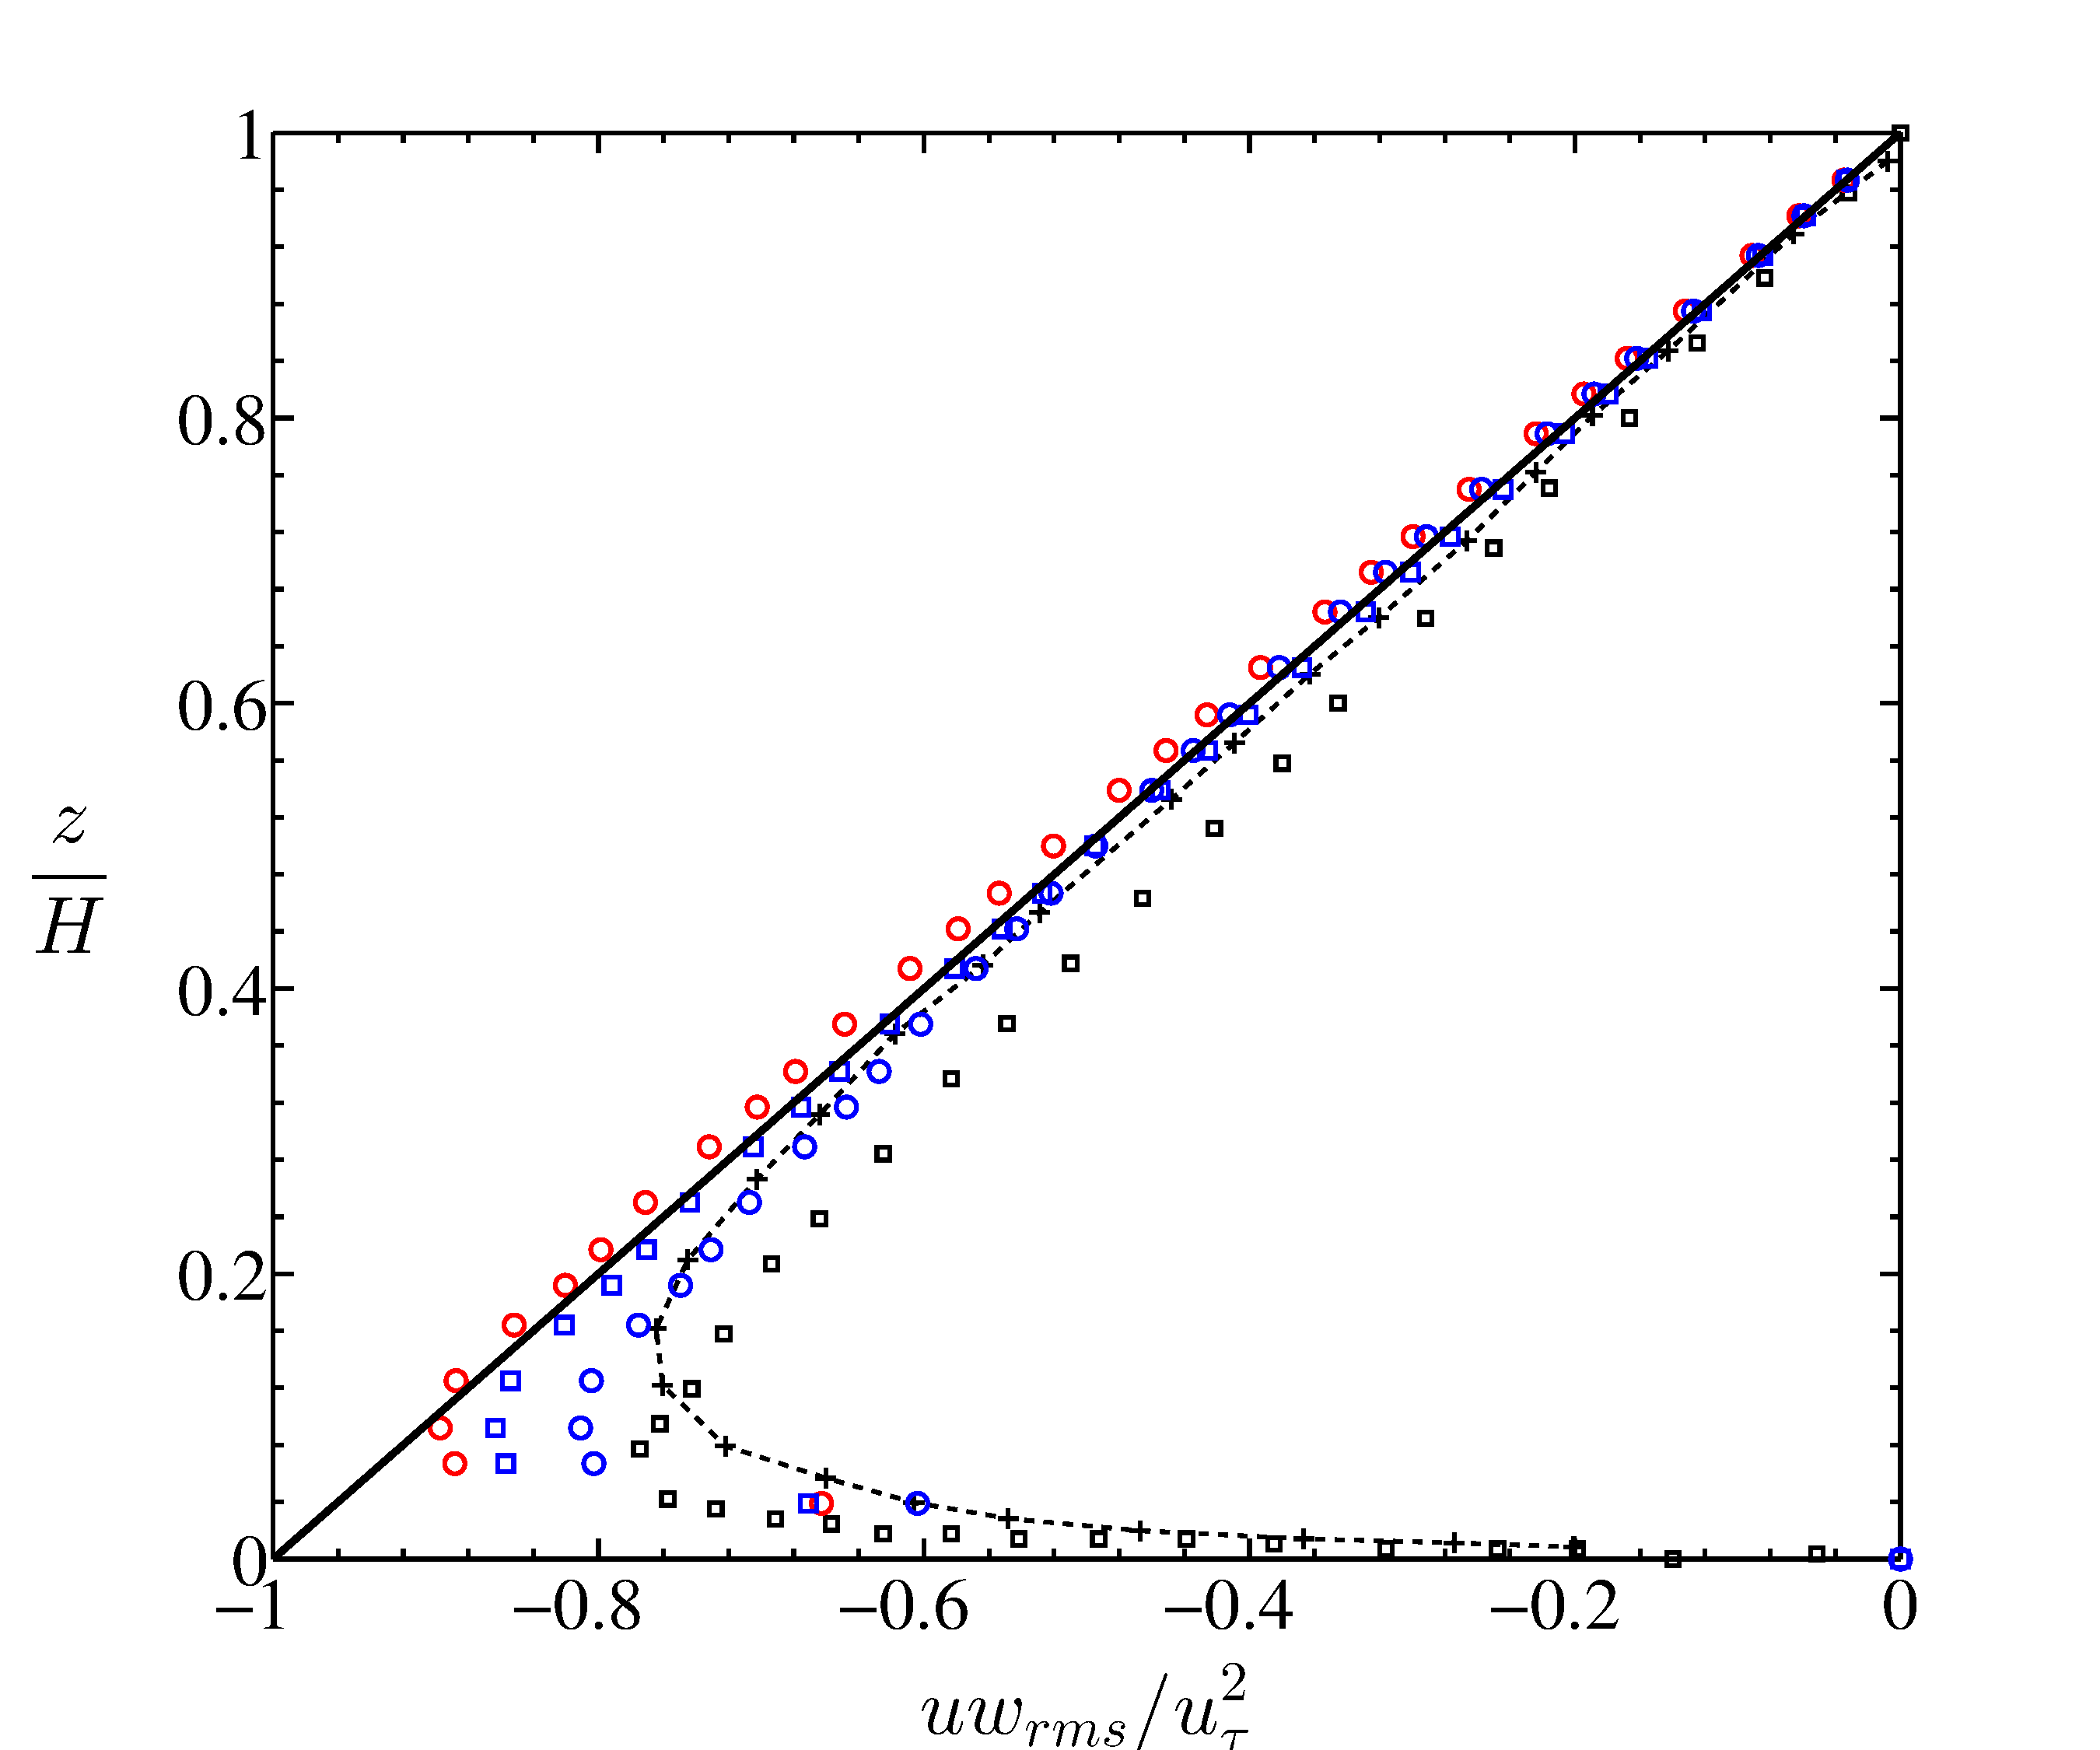
\includegraphics[width=\linewidth]{Fig3/uwrms_filter_n1.pdf}
                \caption{}
                \label{fig:uwrms1a}
        \end{subfigure}%
        \caption[Second order statistics $w_{rms}, \ uw_{rms}$, Case $V-VII$]{Second order statistics for ABL simulations: Case $V-VII$ . (a) $w_{rms}$ (b) $uw_{rms}$ . Red, Blue curves: current simulations $V-VII$ ($n = 1, \ C_0 = 0.17$);  Red $\circ$, $k_{c}=2$; Blue $\circ$, $k_{c} = 4$; Blue $\Box$, $k_{c} = 6$.  Black $-+$, standard Smagorinsky ($C_s = 0.10, n = 2$)  {for Port$\acute{e}$-Agel et al.~\cite{porte1fun}} and black $\Box$ scale dependant dynamic Smagorinsky for Port$\acute{e}$-Agel et al.~\cite{porte1fun}. Solid black line in (b) is the ideal linear trend of non-dimensional total stress. }\label{fig:stat022a}
\end{figure}

\subsection{Cases VIII-X}
With the tuning parameters $C_0 = 0.19, n = 0.5$, the law of the wall shows significant improvements in the near wall region as depicted in Figure~\ref{fig:statb} with the maximum log-law deviation suppressed to 5\% in the lower $10\%$ of ABL. The results are found to be quite comparable with the scale-dependant models of Porte-Ag\'{e}l et. al~\cite{porte1fun} and Bou-Zeid et. al~\cite{bou1} especially with $k_c = 4$. Specifically, {our} results at {$z/H\preceq 0.1$} 
%are exactly intermediate 
{lie in the middle}
between planar averaged scale dependant model of Porte-Ag\'{e}l and its superior Lagrangian averaging counterpart~\cite{bou1}. The plots of $k_c = 2,4,6$ are {practically} indifferent in the near wall region $z/H \sim 0.05-0.1$, beyond which significant differences are registered. For higher explicit filtering with $k_c = 6$, there is a slight negative value of the gradient $\Phi$ at $z/H \sim 0.01$ even though the error is still within $10\%$. The filtering results do not show {significant conspicuousness} in the ``wake-region" except for $k_c = 4$. (The wake region starts at $z/H \sim 0.3-0.4$, when $\Phi(z) > 1$ ). The mean velocity profile gradually decays to {flat profile} with zero gradient as it approaches the top symmetry boundary conditions.{It is observed that in Cases VIII-X, the decay from wake profile to flat profile occurs quite quickly as opposed to a relatively suppressed decay in Cases I-IV.} 
The second order statistics are shown in Figure~\ref{fig:stat021},~\ref{fig:stat022}. The results shows reasonable similarity and sometimes over-prediction of the resolved Reynolds stresses compared to the dynamic Smagorinsky model. {It is quite intriguing to note that a simple change of the shape function of the Smagorinsky mixing length (increasing $dC_s/dz$) has profound impact on the near wall stresses, especially, $u_{rms}, v_{rms}$ which instead of decaying to zero at `` {wall} " for Cases I-IV, actually show a peak at the approximate `` \textit{wall} " similar to the trends of standard dynamic models.}  The results with $k_c=6$ show similar effects of diffusion and {under-prediction of peaks as in case $I-IV$ compared to other values of $k_c$,}  even though the underprediction is much more benign than the previous cases.

\begin{figure}
\centering
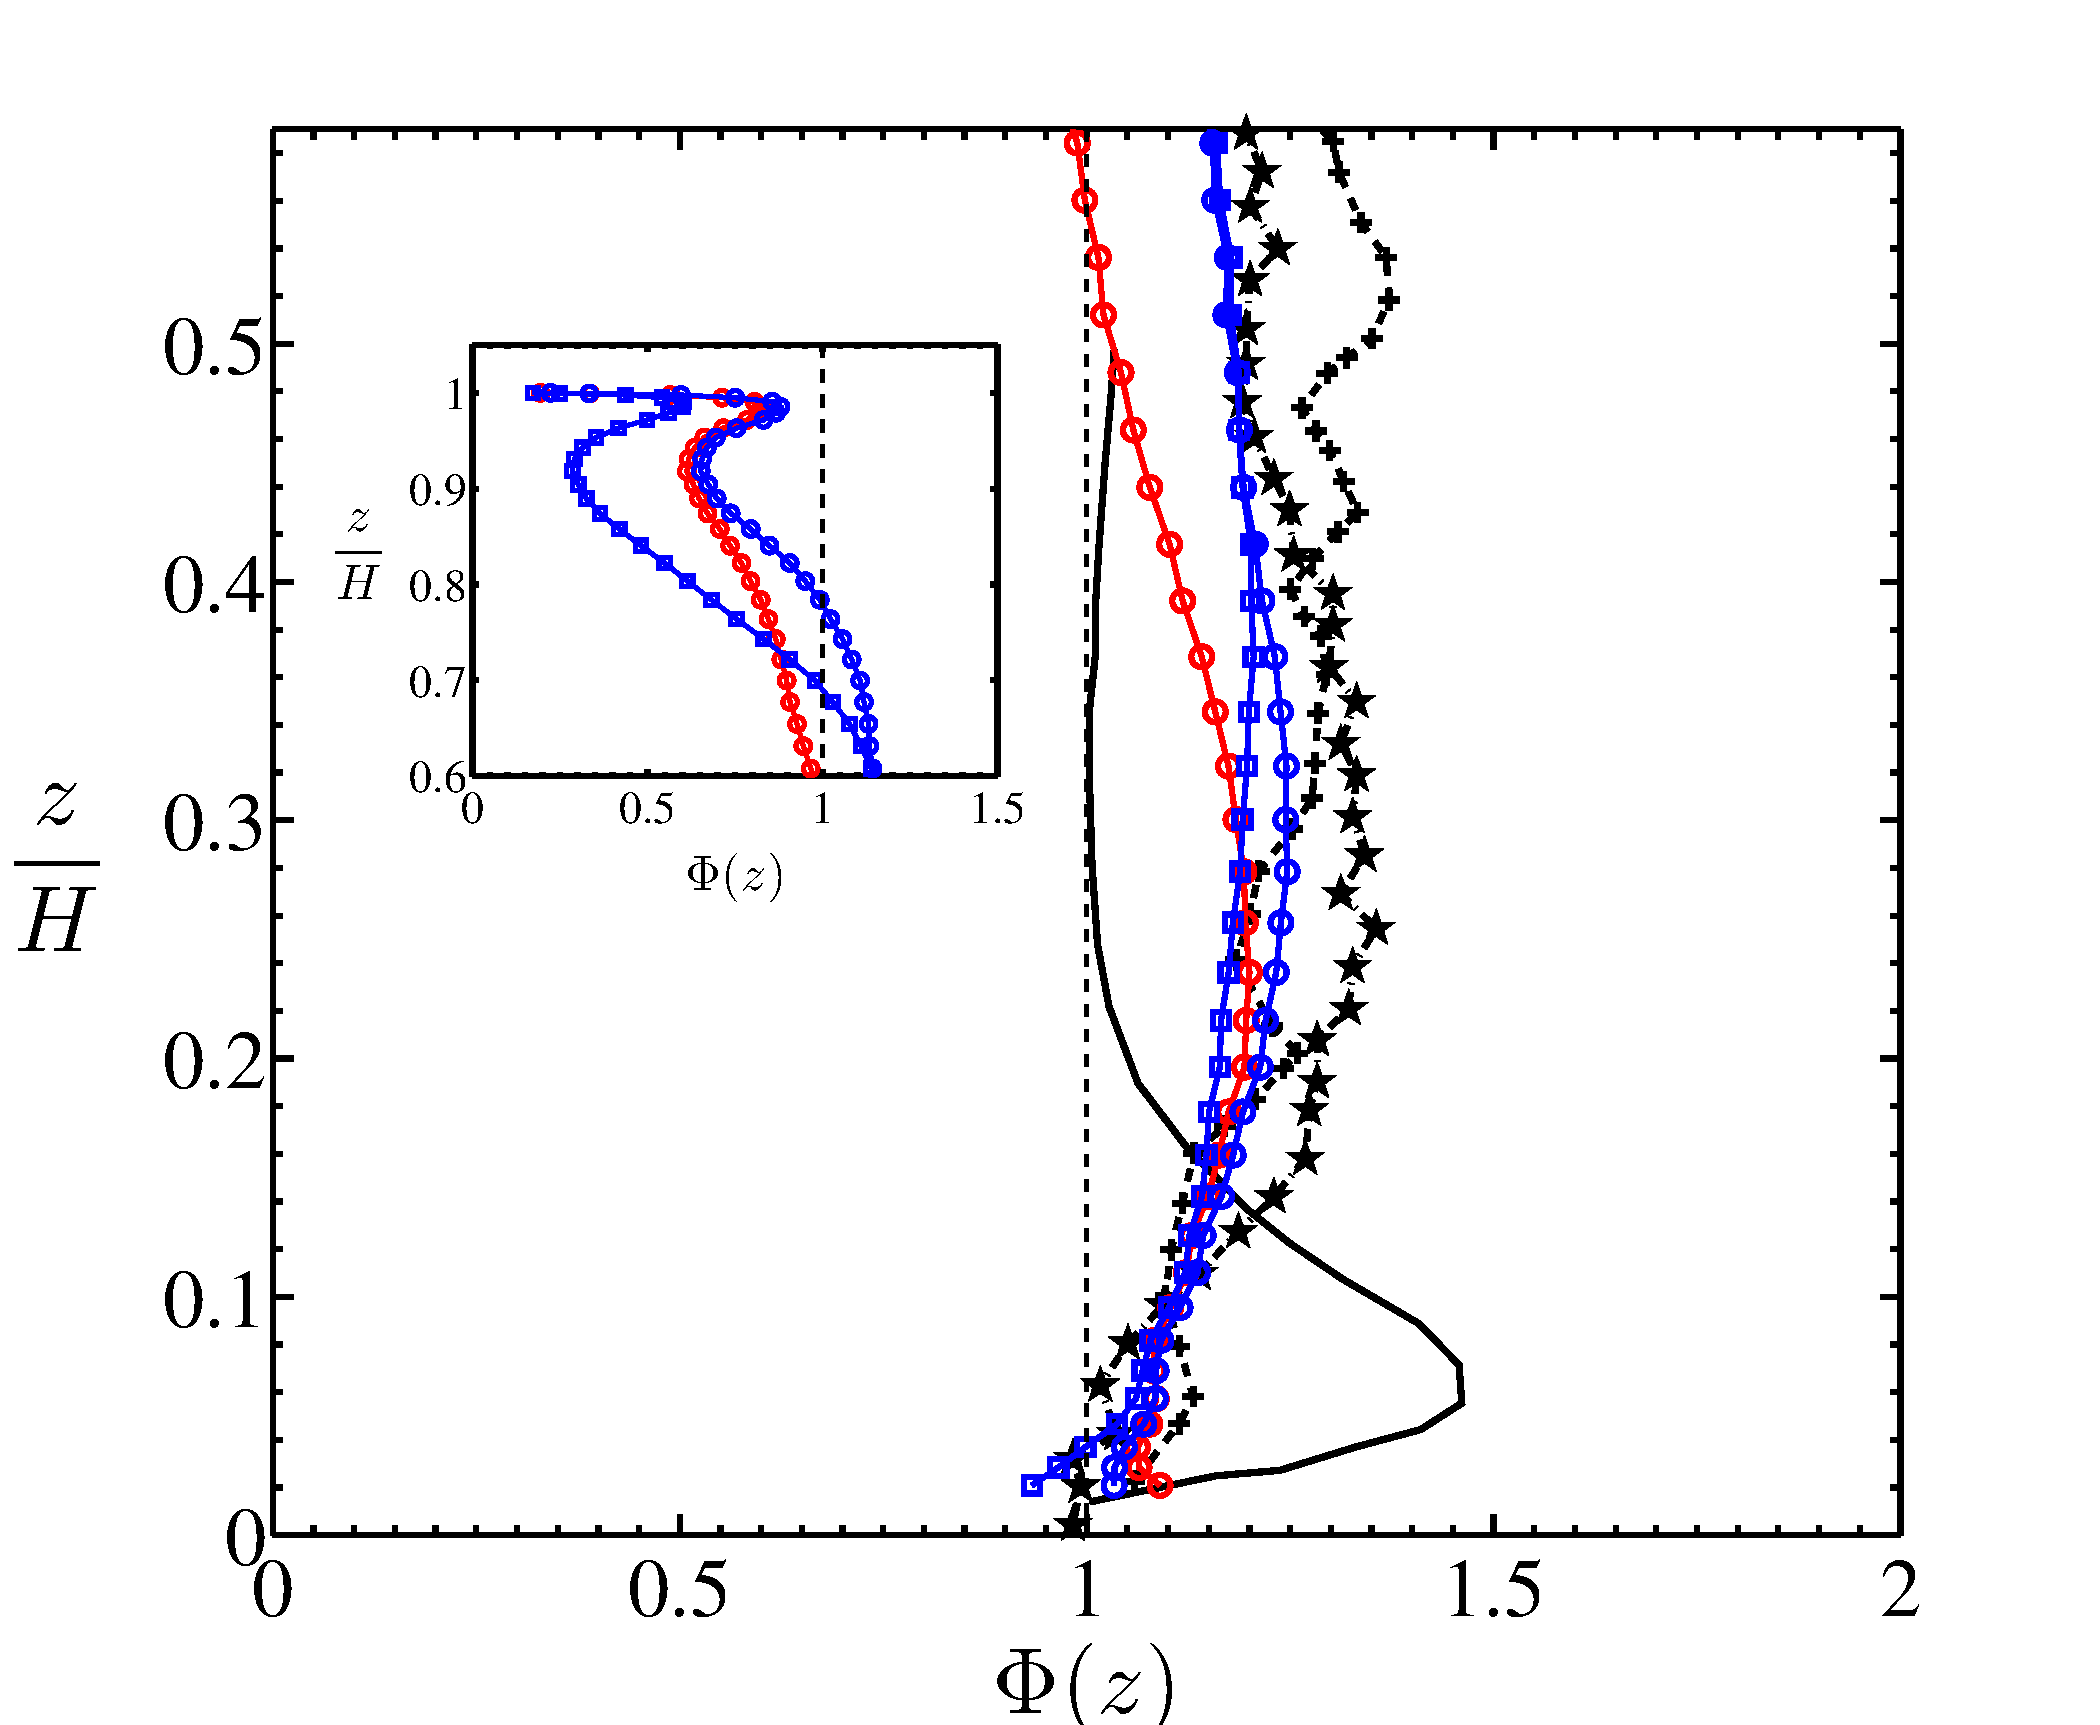
\includegraphics[width = 0.75\linewidth]{Fig3/gradient_filt_n05.pdf}        
        \caption[$\Phi(z)$, Case $VIII-X$]{Non dimensinonal mean streamwise velocity gradient $\phi(z)$ vs $z/H$. Red, Blue curves: current simulations $VIII-X$ {($n = 0.5, \ C_0 = 0.19$)}; Black curves from the literature~\cite{porte1fun,bou1}. Red $\circ$, $k_{c}=2$; Blue $\circ$, $k_{c} = 4$; Blue $\Box$, $k_{c} = 6$. Black $+$ scale dependant dynamic Smagorinsky for Port$\acute{e}$-Agel et al.~\cite{porte1fun}; $-$ , standard Smagorinsky, $\star$, Lagrangian scale dependant dynamic Smagorinsky with filtering, Bou-Zeid et. al~\cite{bou1}}\label{fig:statb}
\end{figure}

\begin{figure}
\centering
        \begin{subfigure}[t]{0.75\textwidth}
                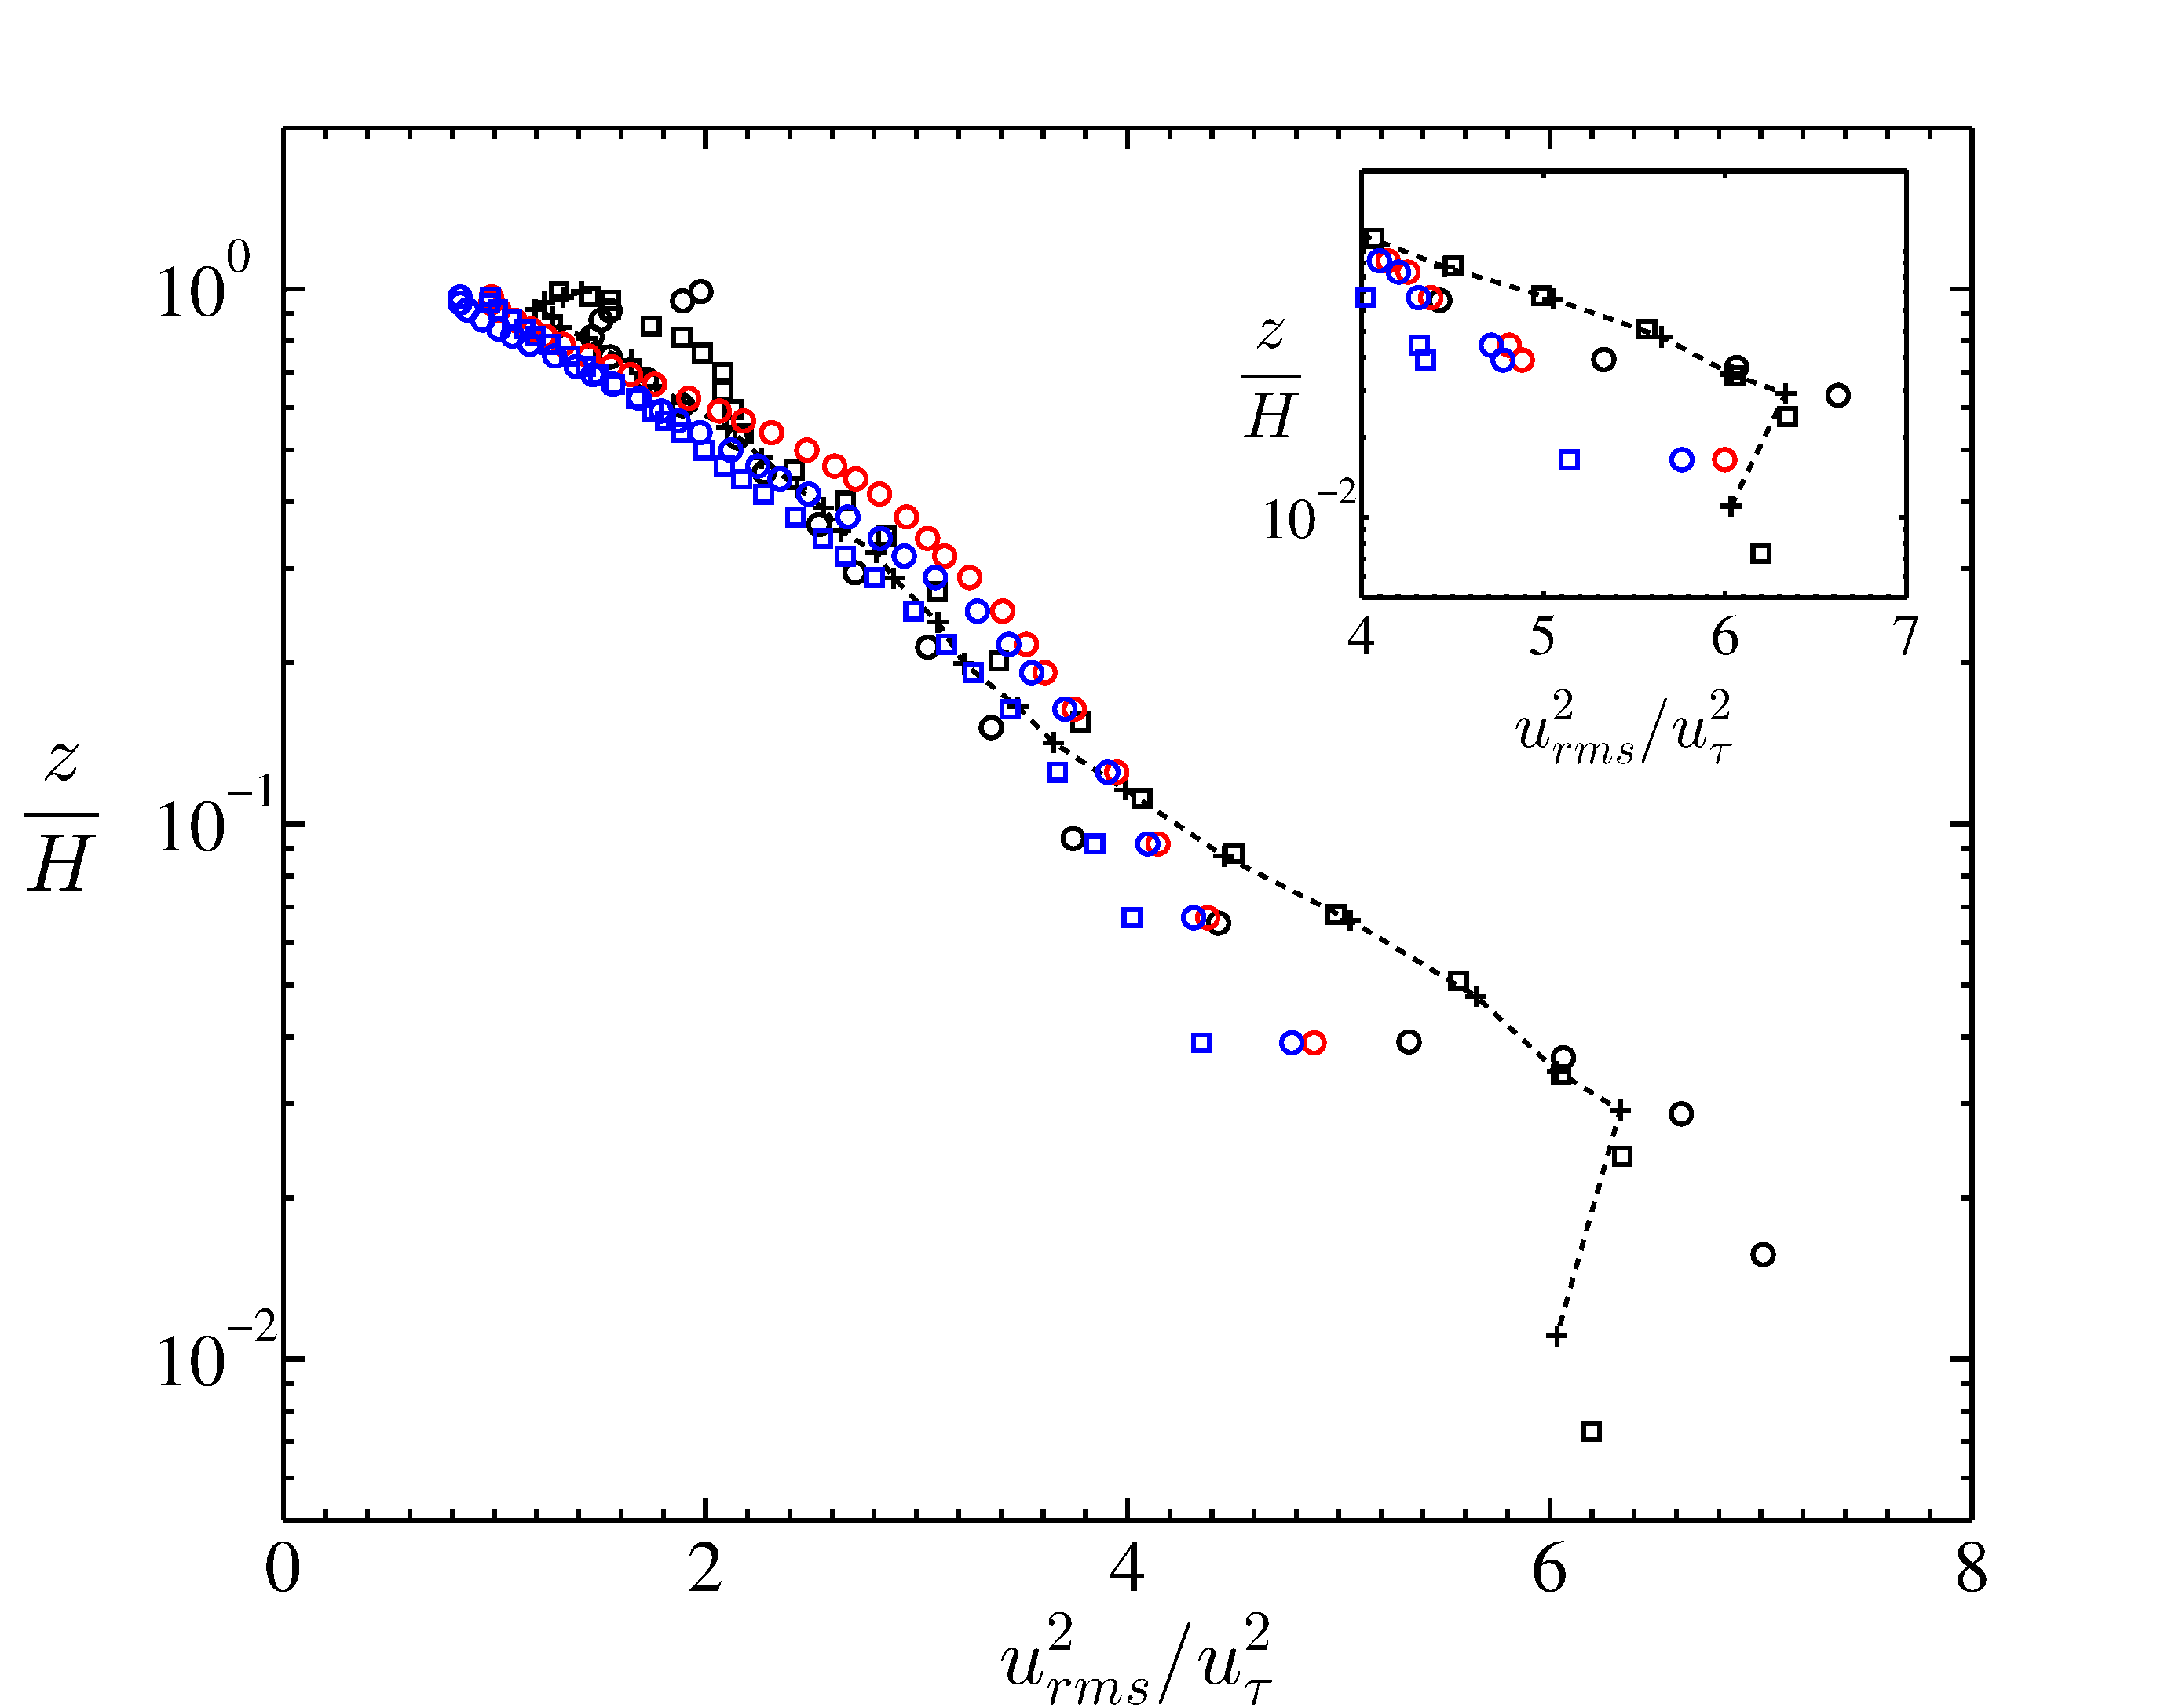
\includegraphics[width=\linewidth]{Fig3/urms_filter_n05.pdf}
                \caption{}
                \label{fig:urms1}
        \end{subfigure}
        \centering
        \begin{subfigure}[t]{0.75\textwidth}
                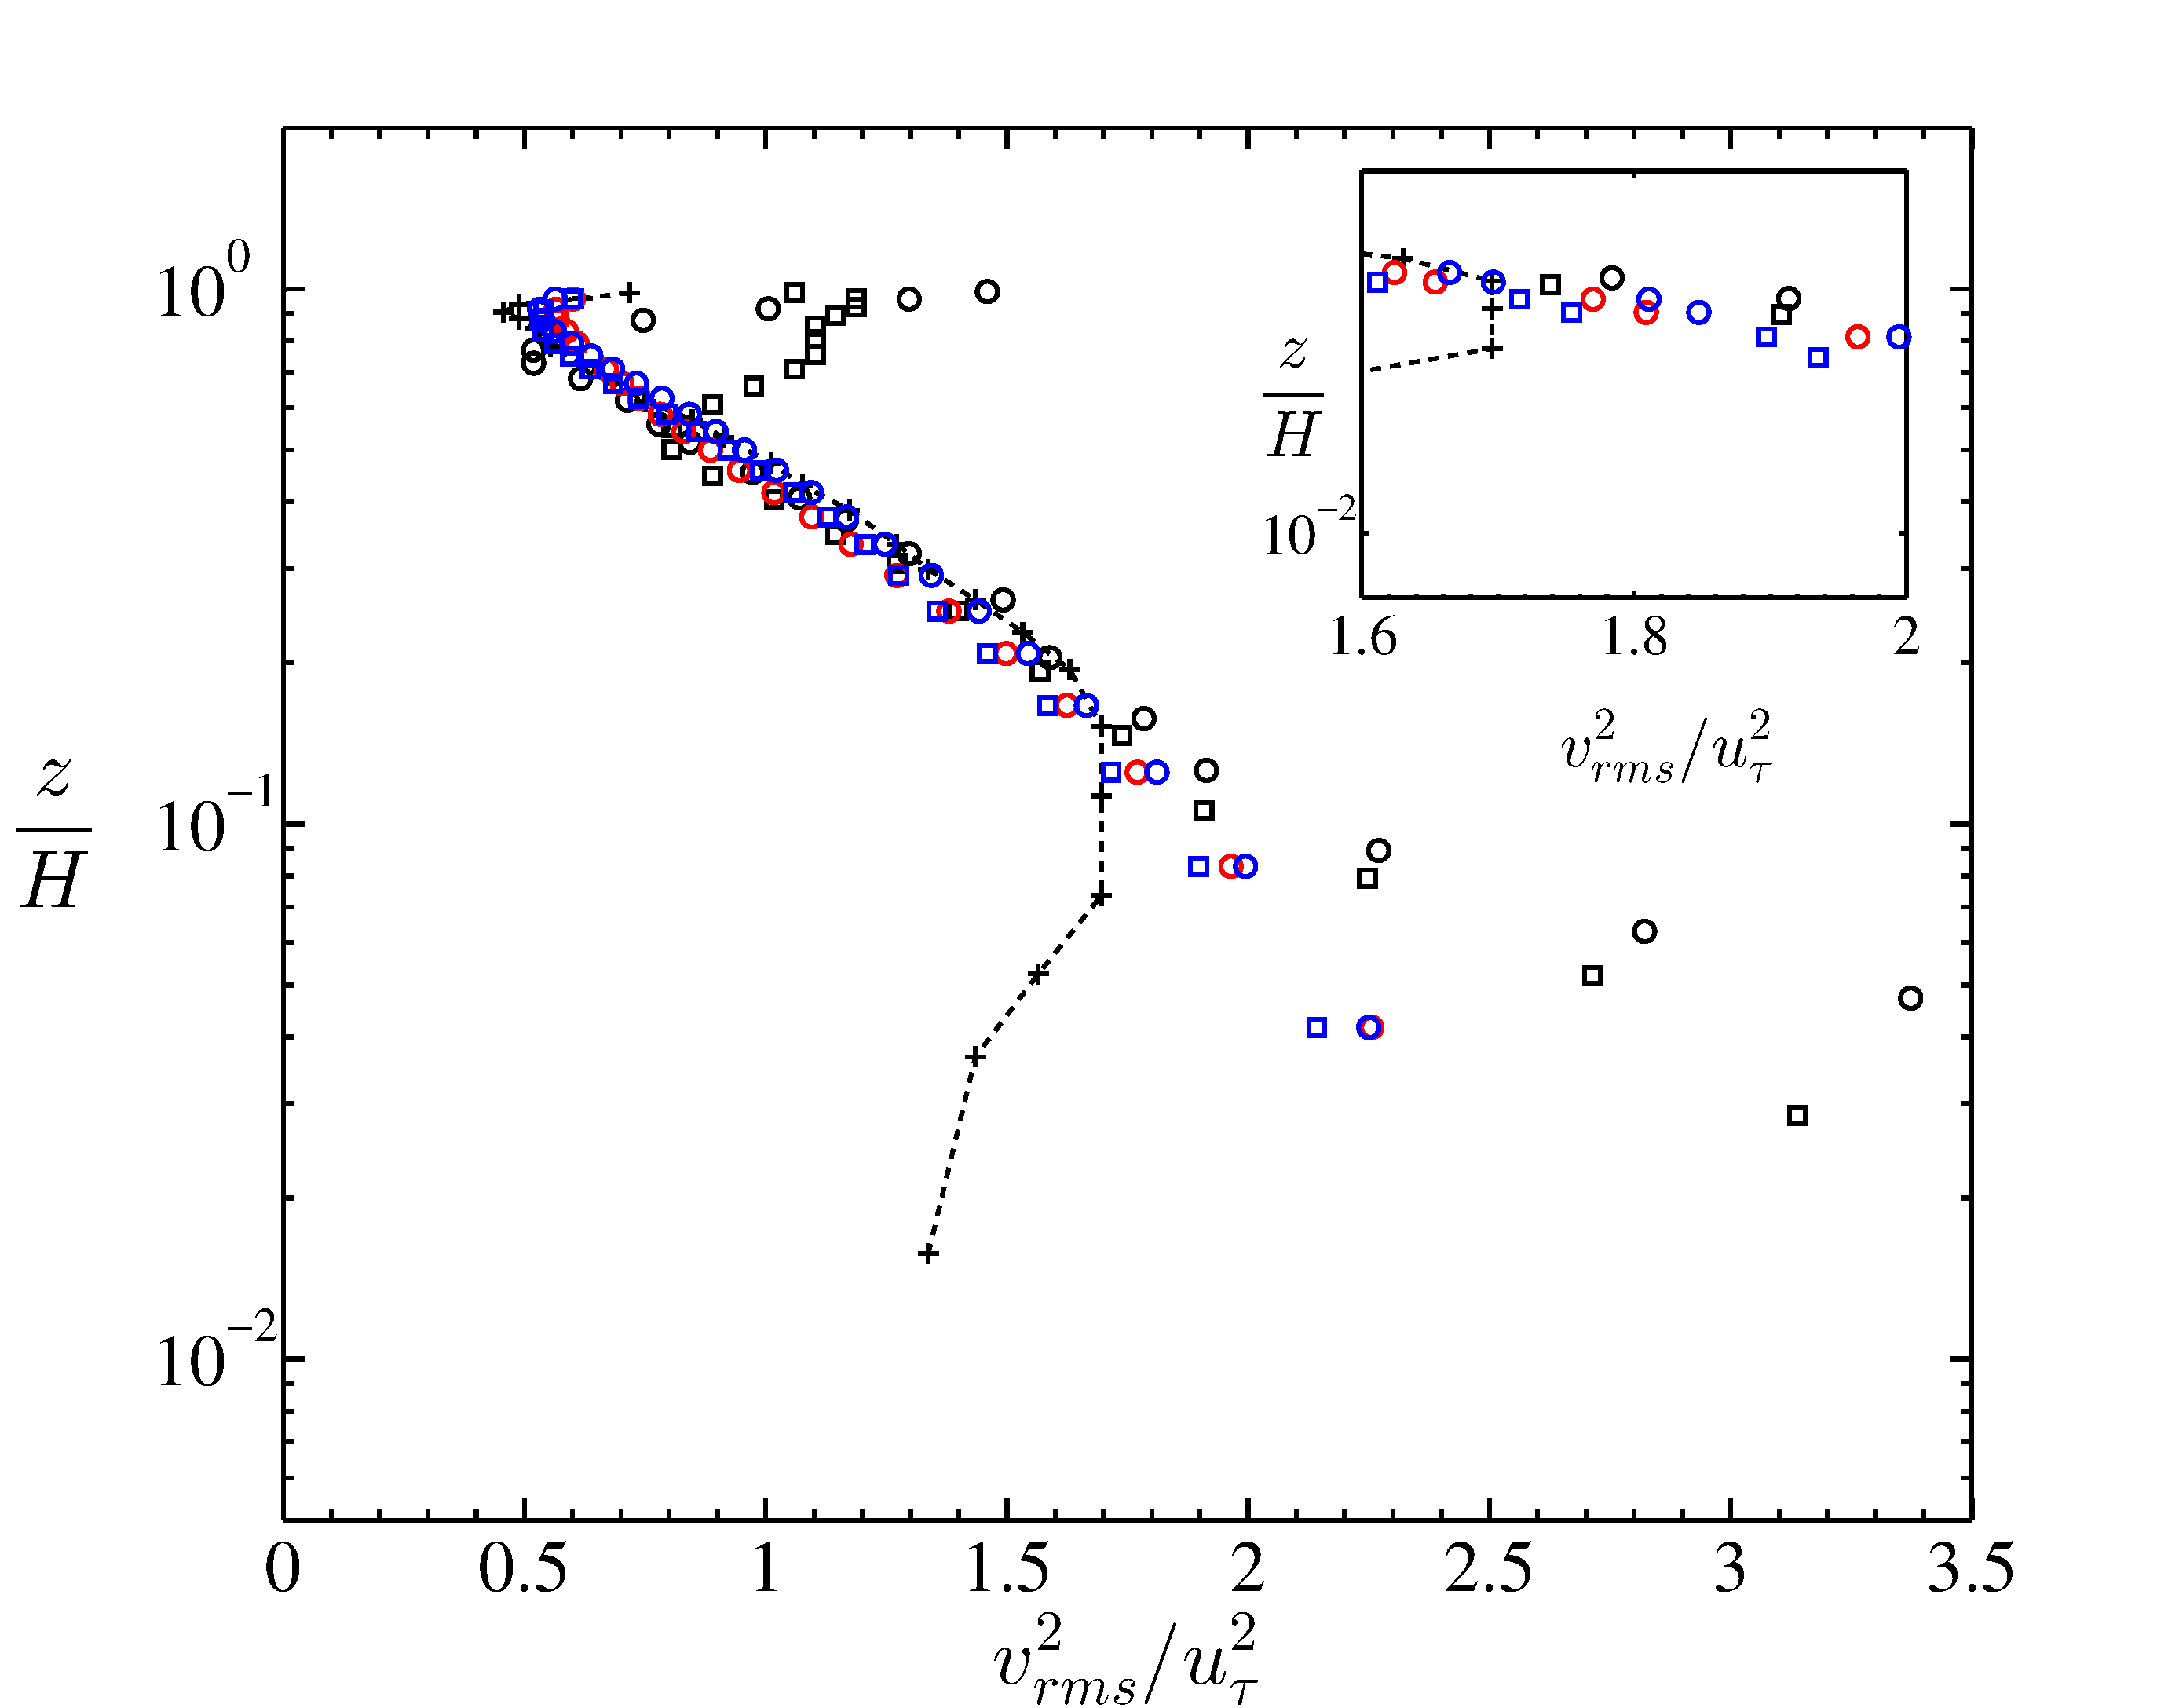
\includegraphics[width=\linewidth]{Fig3/vrms_filter_n05.pdf}
                \caption{}
                \label{fig:vrms1}
        \end{subfigure}
        \caption[Second order statistics $u_{rms}, \ v_{rms}$, Case $VIII-X$]{Second order statistics for ABL simulations: Case $VIII-X$ . (a) $u_{rms}$ (b) $v_{rms}$ . Red, Blue curves: current simulations $VIII-X$ ($n = 0.5, \ C_0 = 0.19$);  Red $\circ$, $k_{c}=2$; Blue $\circ$, $k_{c} = 4$; Blue $\Box$, $k_{c} = 6$.  Black $-+$, standard Smagorinsky ($C_s = 0.10, n = 2$)  {for Port$\acute{e}$-Agel et al.~\cite{porte1fun}} and black $\Box$ scale dependant dynamic Smagorinsky for Port$\acute{e}$-Agel et al.~\cite{porte1fun}.}\label{fig:stat021}
\end{figure}
\begin{figure}
        \centering
        \begin{subfigure}[t]{0.75\textwidth}
                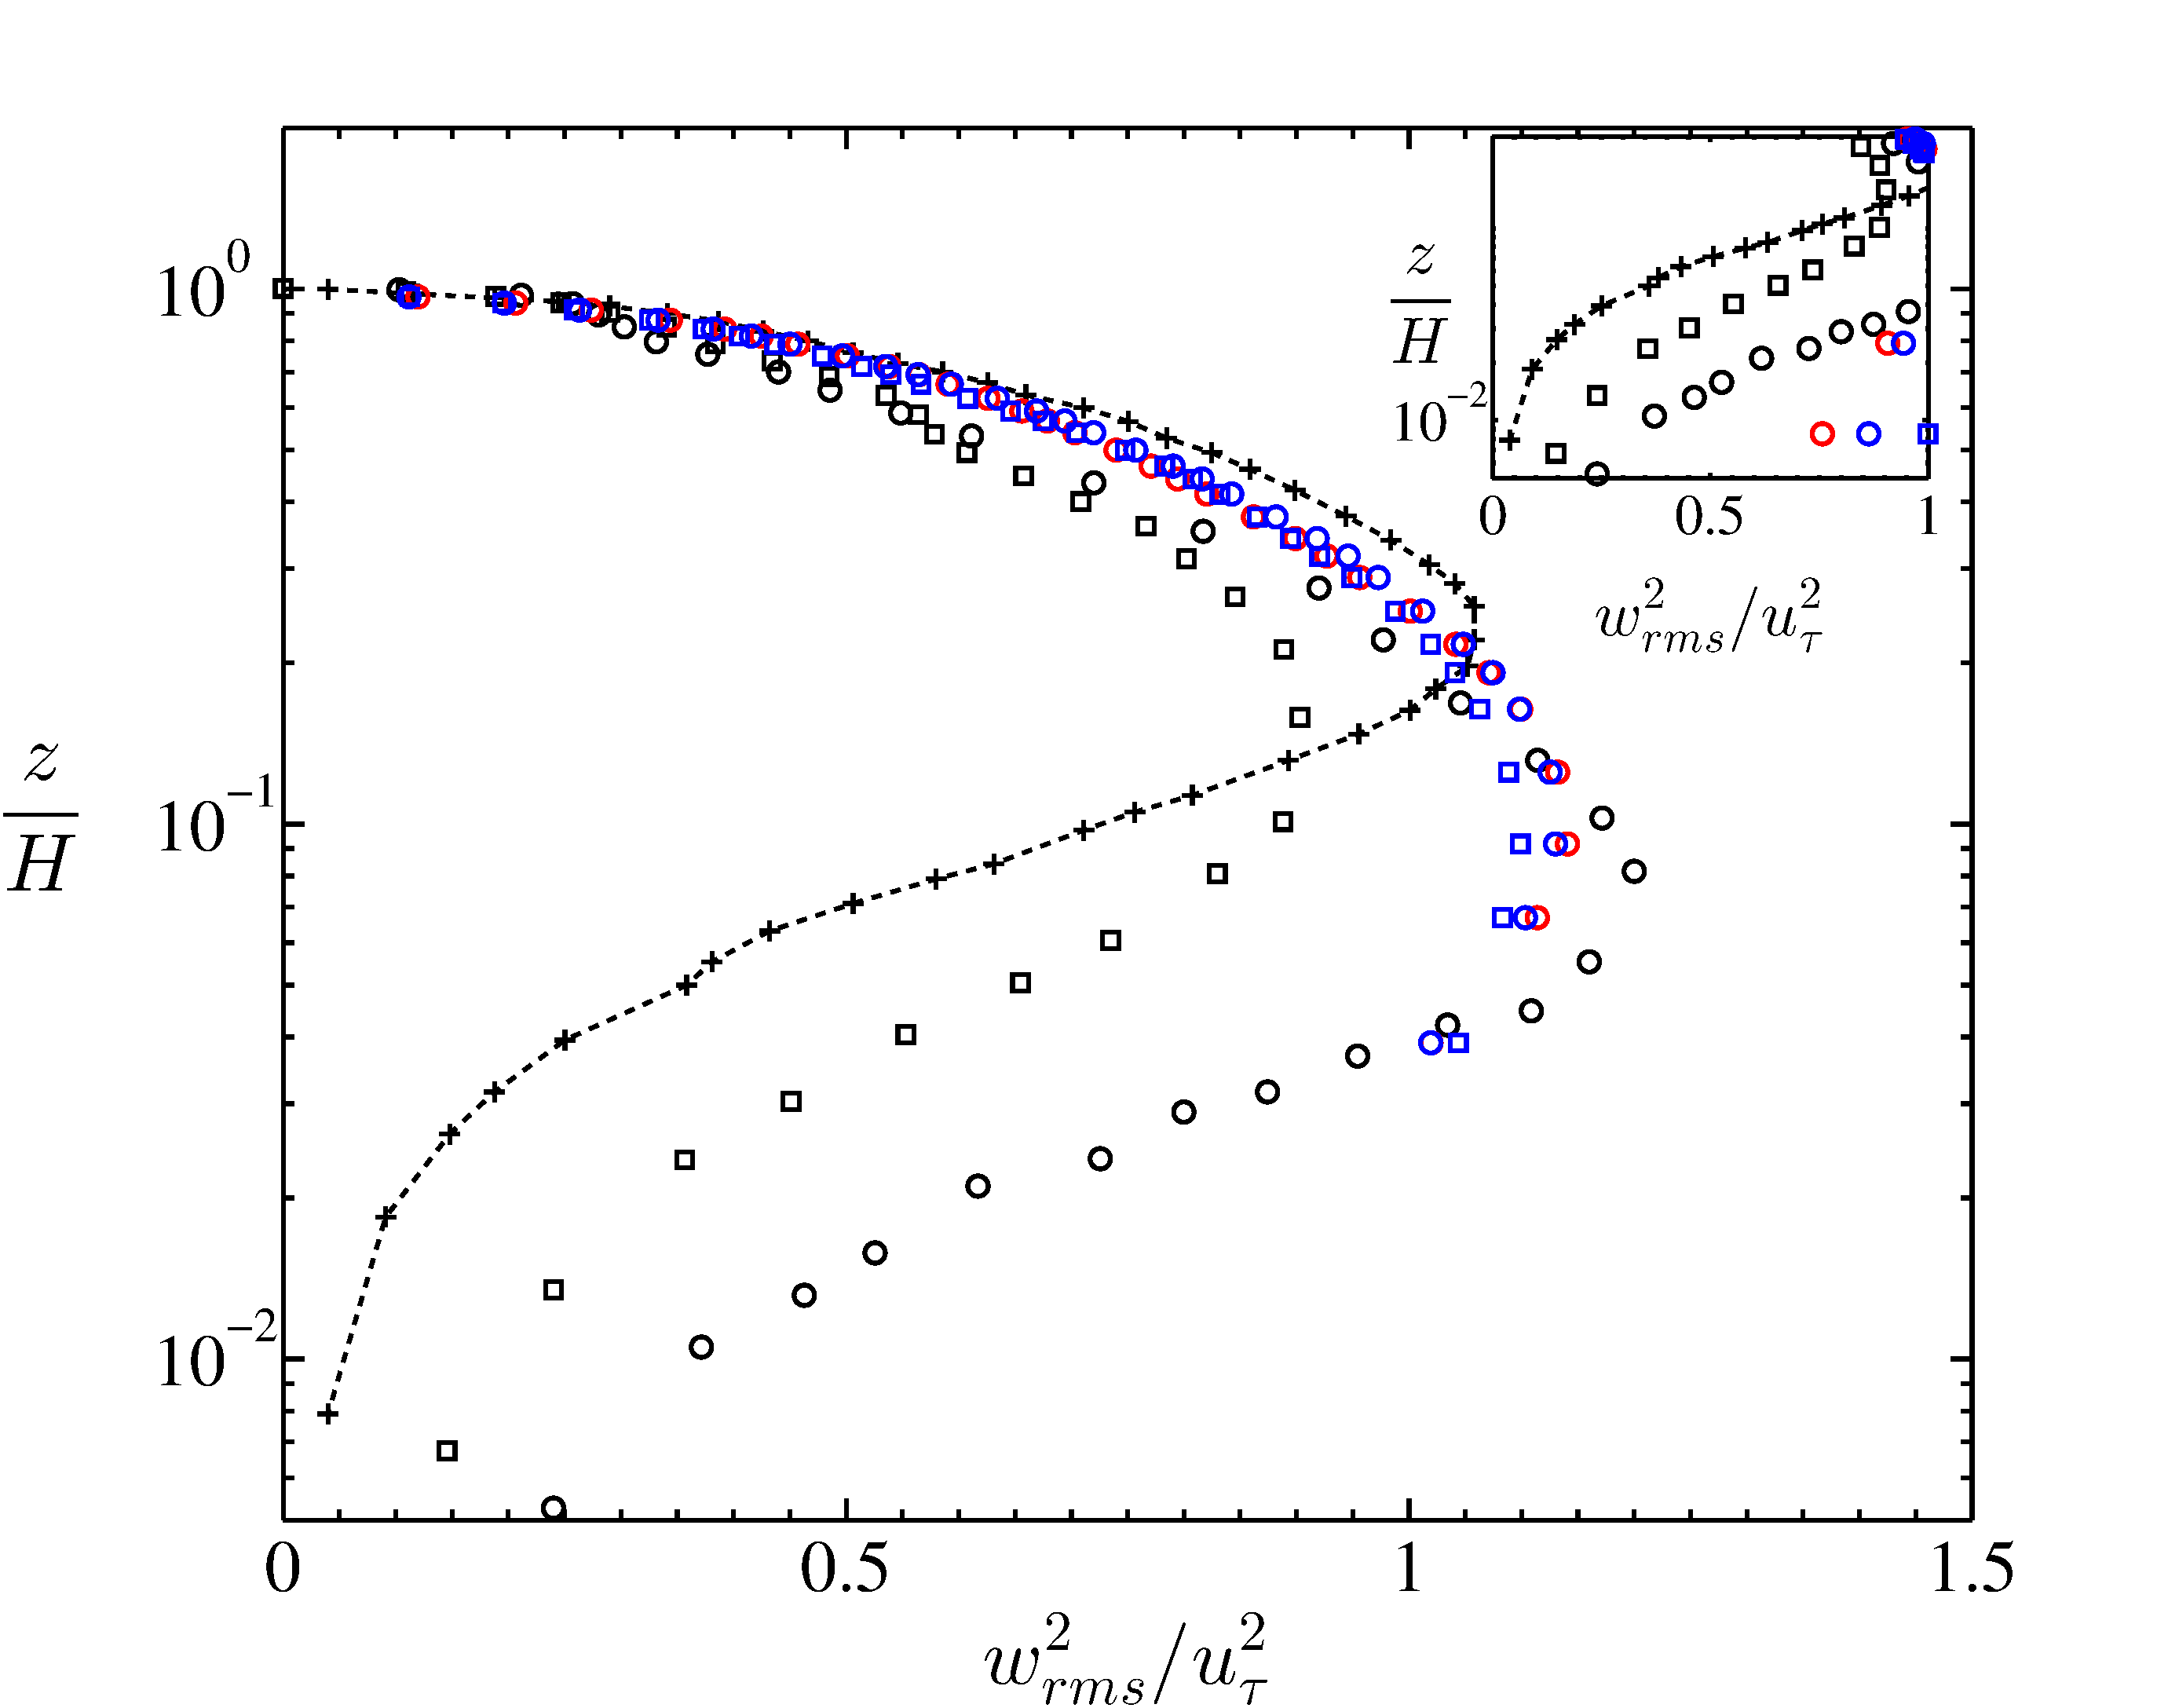
\includegraphics[width=\linewidth]{Fig3/wrms_filter_n05.pdf}
                \caption{}
                \label{fig:wrms1}
        \end{subfigure}
        \centering
        \begin{subfigure}[t]{0.75\textwidth}
                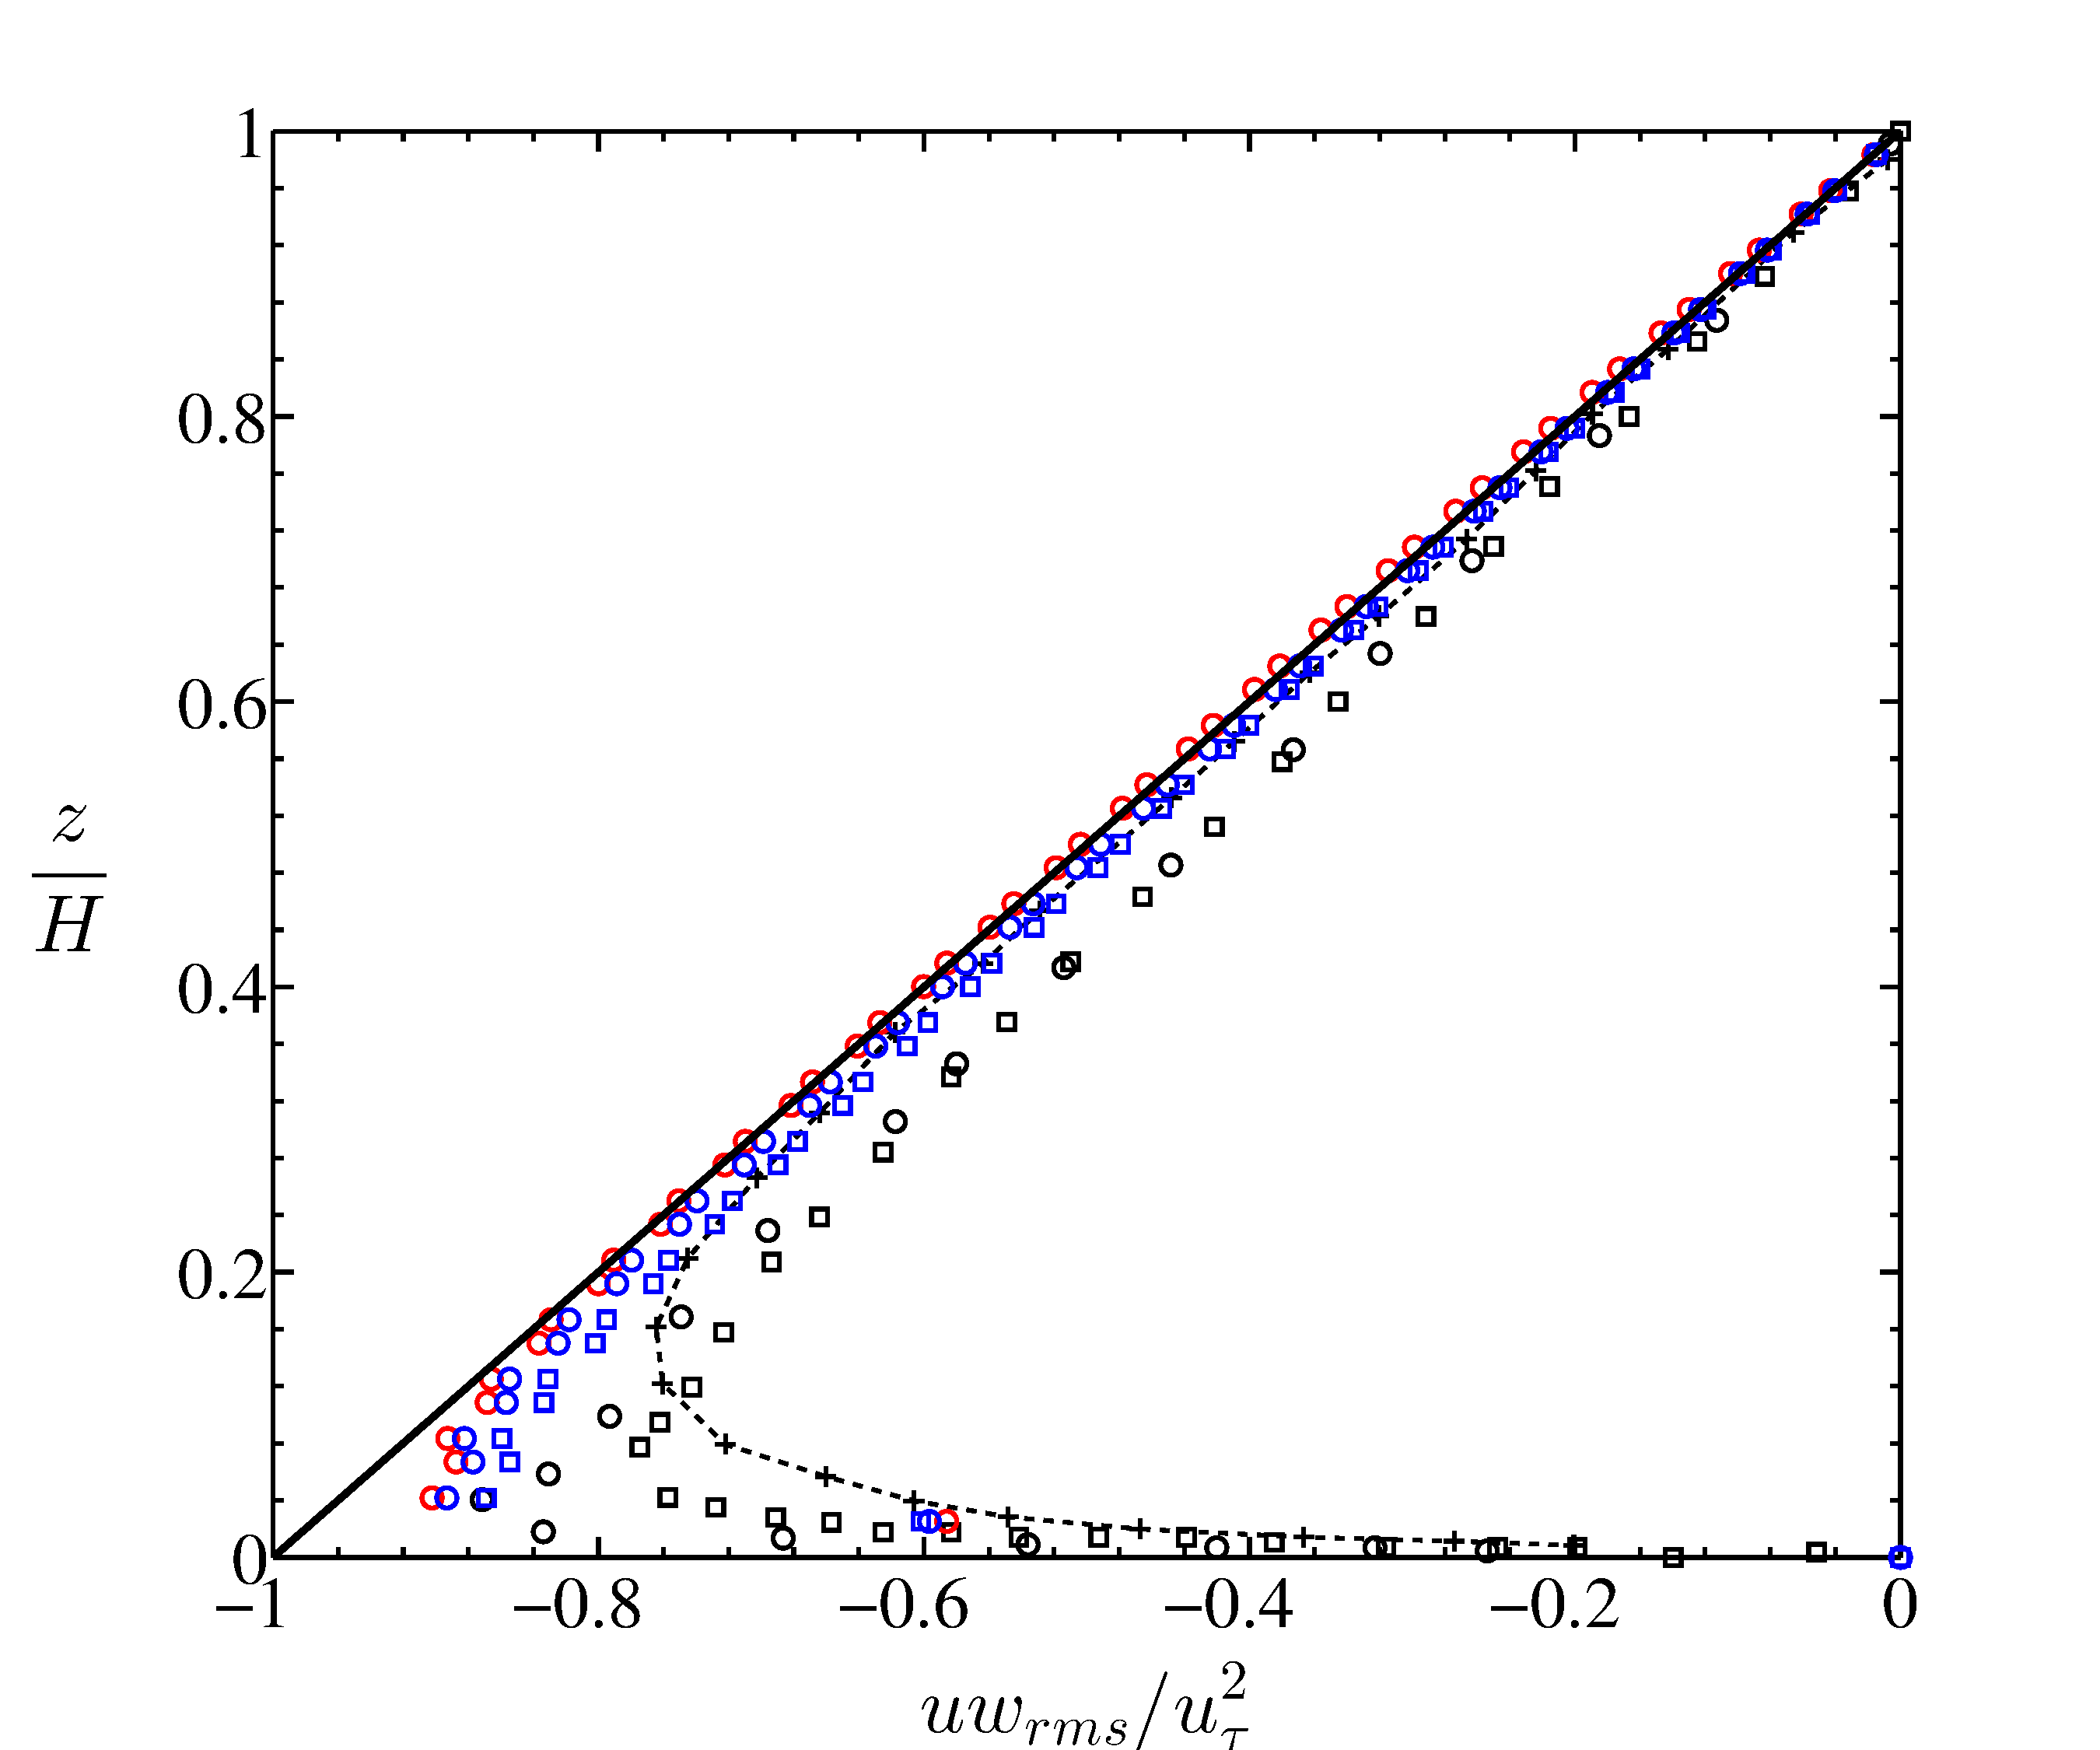
\includegraphics[width=\linewidth]{Fig3/uwrms_filter_n05.pdf}
                \caption{}
                \label{fig:uwrms1}
        \end{subfigure}%
        \caption[Second order statistics $w_{rms}, \ uw_{rms}$, Case $VIII-X$ ]{Second order statistics for ABL simulations: Case $VIII-X$ . (a) $w_{rms}$ (b) $uw_{rms}$ . Red, Blue curves: current simulations $VIII-X$ ($n = 0.5, \ C_0 = 0.19$);  Red $\circ$, $k_{c}=2$; Blue $\circ$, $k_{c} = 4$; Blue $\Box$, $k_{c} = 6$.  Black $-+$, standard Smagorinsky ($C_s = 0.10, n = 2$) {for Port$\acute{e}$-Agel et al.~\cite{porte1fun}} and black $\Box$ scale dependant dynamic Smagorinsky for Port$\acute{e}$-Agel et al.~\cite{porte1fun}. Solid black line in (b) is the ideal linear trend of non-dimensional total stress.}\label{fig:stat022}
\end{figure}

\subsection{A note on Log Layer Mismatch}\label{lotw}
The term ``log-layer mismatch" has been found in the papers by Brasseur {and Wei}~\cite{brass},  Wu $\&$ Meyers~\cite{meyers_err} and Meyers~\cite{meyers2} but {its} detrimental effects have been seen in all LES results of high Reynolds number turbulent boundary layer flow~\cite{sull,pio2,porte1fun,bou1,chow,temp2}. The effect of ``log-layer mismatch", as also discussed above, is the deviation of the mean velocity gradient from the expected logarithmic trend in the near-wall region ($\Phi(z) > 1$ and usually shows a peak structure at $z/H < 0.1$), which has been partially addressed by having a proper choice of SGS model~\cite{mason,porte1fun,bou1} or explicit filtering in the wall closure model~\cite{bou1,meyers_err,meyers2} or using more complicated techniques like optimal control theory~\cite{temp2}, designing high accuracy zones for law of {the} wall~\cite{brass} or blending functions in self-adaptive models~\cite{meyers2} .
To understand the fundamental cause of "log-layer mismatch" we resort to Figure~\ref{fig:hiRe} where we plot $\Phi(z) = \kappa z/u_{\tau} dU/dz$ vs $z/\delta$, for high $Re$ channel flow DNS~\cite{lee2} with $\delta$ being the half channel width. We note, that  similar peaked structures in Figure~\ref{fig:hiRe} (we would call them ``log law deviation" subsequently to differentiate between "log-layer mismatch" in ABL) can be seen, as we have  observed in Figures~\ref{fig:stata},~\ref{fig:statba} for rough-wall neutral atmospheric boundary layer for high $Re$. It is not hard to relate those deviations from $\Phi(z) = 1$ in Figure~\ref{fig:hiRe}, due to the presence of physical viscous sub-layer where log-law does not hold. With increasing $Re_{\tau}$, there is an increasing separation of outer and inner scales $\delta/\delta_{\nu}$~\cite{pope,balad}, where $\delta_{\nu} = \nu/u_{\tau}$. Consequently, since $\delta$ is fixed in all DNS simulations (Figure ~\ref{fig:hiRe}), increasing $Re_{\tau}$ would require the shrinkage of inner scales $\delta_{\nu}$, which does not minimize the``log-law deviations" at all but rather makes the peaks of those deviation thinner and  shifts them more towards the wall in outer scale $z/\delta$, while the peaks remain at the same locations with same magnitudes in the inner scale $z^{+}$, normalized with $\delta_{\nu}$. Consequently, the more the peak shifts towards the wall, the more quickly $\Phi(z)$ becomes closer to 1, i.e. at much lower value of $z/\delta$.  It is thus not surprising that in standard Smagorinsky model (dissipative SGS model) with constant $C_s$ or also sometimes with wall-damped $C_s$~\cite{mason,chow} for very high $Re$ we would observe similar log-law deviations due to the presence ``unphysical / artificial viscous sublayer" with a representative length scale $\delta_{\nu_t}$, where $\nu_{t} = (C_s\Delta)^{2}\vert \widetilde{S} \vert$ is the Smagorinsky eddy viscosity. Also, the location of such peaks would scale well with $\delta_{\nu_{t}} = \nu_{t}/u_{\tau}$. Similar feature as in the argument above can actually be seen through careful observation of Figure~\ref{fig:stata},~\ref{fig:statba}. The peaks of the log-layer mismatch in those figure (current spectral element simulations) are actually closer to the wall compared to the standard Smagorinsky model of Bou-Zeid et. al~\cite{bou1}. This can be attributed from the fact that the length-scale in the artificial viscous sublayer is much smaller (contributed only by the Smagorinsky model, numerical dissipation negligible) while for~\cite{bou1} $\delta_{\nu_t}$ is much larger (probably due to the contribution of numerical dissipation and higher Smagorinsky coefficient). Additionally it can be understood, that as long as the artificial boundary layer can be formed, with eddy viscosity $\nu_t$, the log-layer mismatch would persist irrelevant of the fact whether $nu_{t}$ is small or big. This is corroborated in the papers of Khanna and Brasseur~\cite{khan} and Spalart~\cite{spal2}, who observed that refining vertical resolution actually shifted the ``log-layer mismatch" downards towards the wall which can be attributed to the decrement yet persistance of the numerical dissipation in the grid. (similar as in Figure~\ref{fig:hiRe}) It is only with a careful design of $nu_{t}$, we can stop the artificial / unphysical layer to form itself, resulting in proper log-layer predictions. These ideas are along the lines of the Log-law analysis made by Brasseur and Wei~\cite{brass}, and can be referred for further details. A quick calculation of  the parameters $\mathfrak{R}-R_{LES}-N_{\delta}$ in Table~\ref{table:brass} as suggested by Brasseur and Wei~\cite{brass} along with their critical values have been registered. The parameters (See details in~\cite{brass}) should be greater than the critical values to avoid log-layer mismatch, and it is not surprising that only models with $n = 1/2$ and indepedant of the filtering modes $k_c$ consistently qualify their tests and thus can avoid ``log-layer mismatch". The bottom line is simply decreasing of $C_s\Delta$ in the Smagorinsky coefficient would never minimize log-layer mismatch as its origin does not lie on extra-dissipative Smagorinsky model, but rather an unphysical near wall dissipation in the first place. These discussions are corroborated by the fact that the biggest challenge reported in representing the near wall logarithmic trends (also the near-wall features) on a relatively co{a}rse LES grid  is that the {numerical discretization errors} near wall start \textbf{interfering} with the physical modelling and affecting the results of the resolved statistics~\cite{cabot2,brass,meyers2}.  
 %Additionally it was also observed that in the first grid point of the finite difference scheme large errors of velocity gradient deviating from the logarithmic trends crop in, and are alleviated by simply brute forcing the logarithmic gradient at the first grid point~\cite{porte1fun,meyers2}. 
\begin{table}[ht] 
\centering % used for centering table 
\begin{tabular}{c c c c} % centered columns (4 columns) 
\hline\hline    %inserts double horizontal lines 
Case & $\mathfrak{R}$  & $R_{LES}$ & $N_{\delta}$   \\ [0.5 ex] % inserts table 
%heading 
\hline  % inserts single horizontal line 
III & 0.0599 & 436 & 169 \\
VI & 0.1517 & 474 & 169 \\
IX & 1.6454 & 1090 & 169 \\
\hline
VIII & 1.6811 & 1105 & 169 \\
IX & 1.6454 & 1090 & 169 \\
X & 1.5835 & 1064 & 169 \\
\hline \\ [1 ex]
\end{tabular} 
\caption[HAZ parameters of Brasseur and Wei (2010)]{Estimation of three parameters suggested by Brasseur and Wei~\cite{brass} in our current model to estimate the High-Accuracy-Zone. Critical parameters: $\mathfrak{R^{*}} \gtrsim 1$, $R_{LES}^{*} > 350$ and $N_{\delta}^{*} > 45-50$}  % title of Table 
\label{table:brass} % is used to refer this table in the text 
\end{table} 
% May be conclusion: decouple SGS modelling error + Numerical discretization error
To summarize, as pointed out by Brasseur and Wei~\cite{brass}, we would like to emphasize that the persistance of log-scaling is essentially the dominance of intertial scales ($u_{\tau}, z$) over viscous scales (molecular, SGS dissipation/ numerical) and also scales imposed by the roughness element $z_0$. Mismatch would occur, if any other scales, dominates over the inertial scaling. It is at this bottleneck, that the spectral element method plays a crucial role in modelling the high $Re$ turbulent boundary layer flows. Using higher polynomial orders ($\sim 7$) and limited amount of tuning in the SGS models in the current simulations, we can technically put a barrier to the diffusion and dispersion errors (spurious numerical scales) percolating to the physical system involving near wall modelling. Consequently, we could address the effects of ``log layer mismatch" or the generation of an artificial viscous sublayer with a reasonable amount of success {without evoking more sophisticated dynamic-type models}.  {From Figure~\ref{fig:stat0_lotw} we observe that the SGS models with $n = \frac{1}{2}$ show much better logarithmic trends {at $z/H \sim 0.1$} as compared to $n = 1,2,3$ which manifest ``log-layer mismatch".}

\begin{figure}
\centering
\begin{subfigure}[t]{0.5\textwidth}
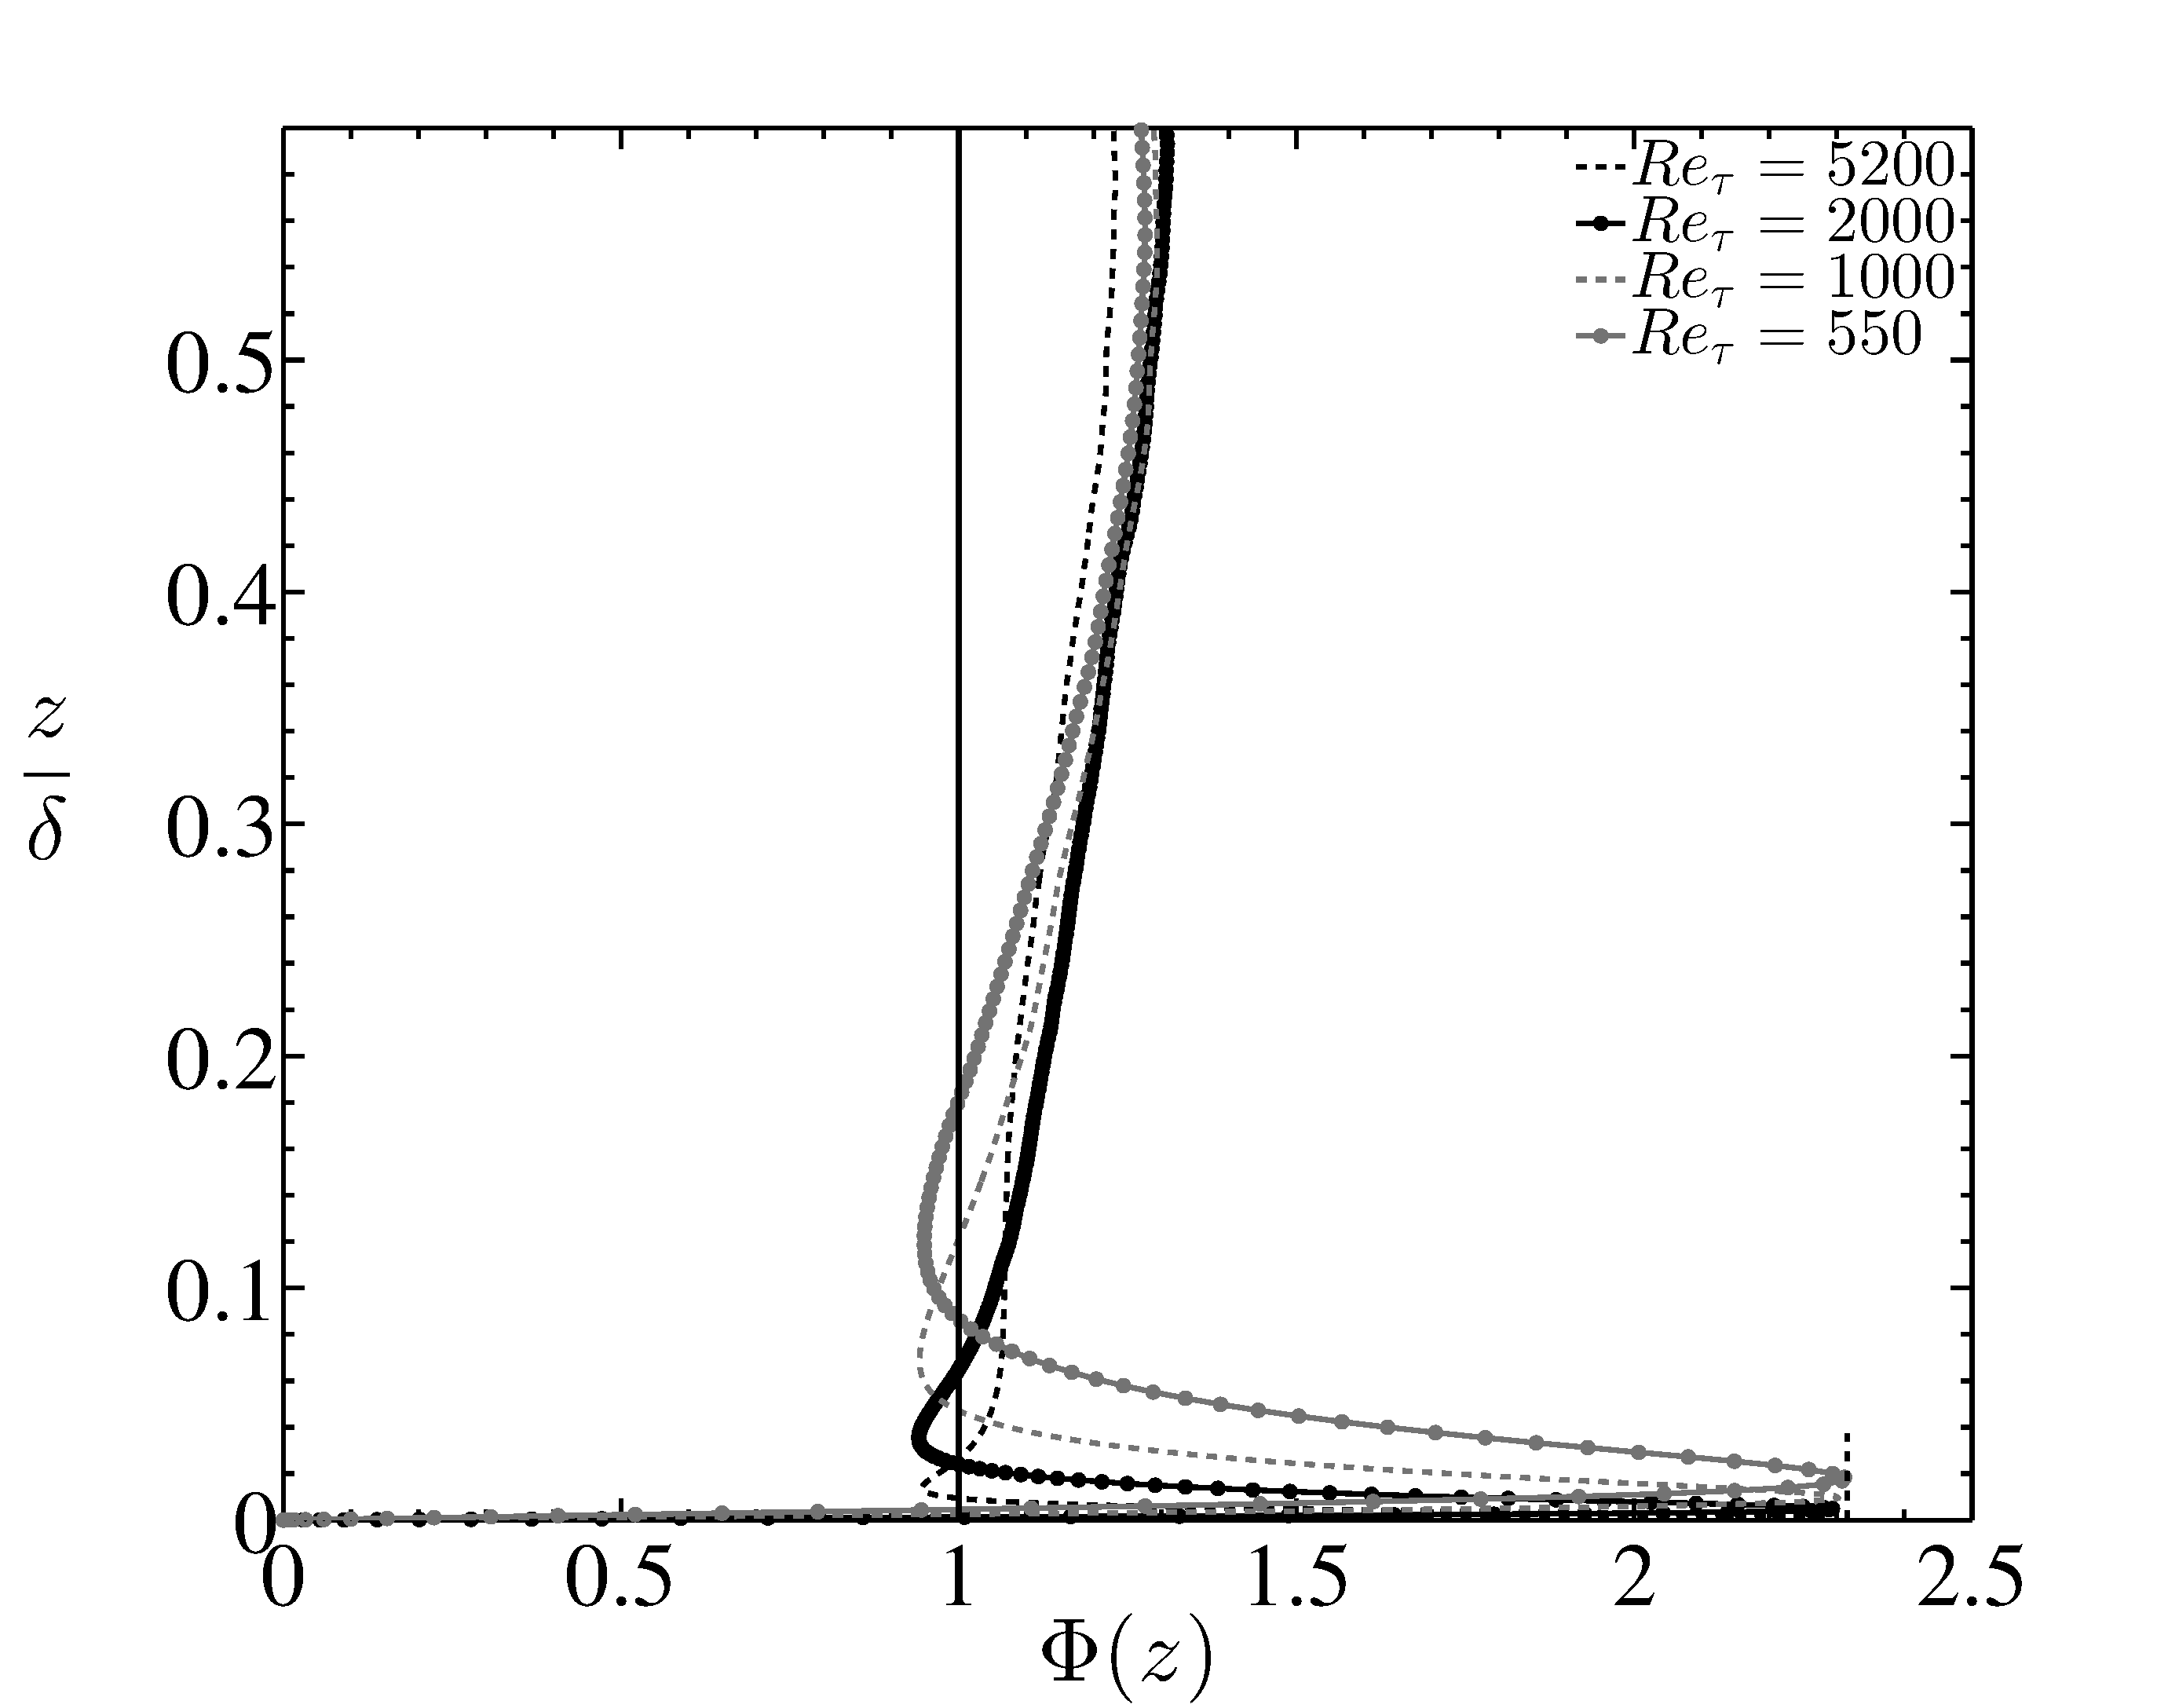
\includegraphics[width = \linewidth]{Figure/highRe.pdf}
\end{subfigure}%
\begin{subfigure}[t]{0.5\textwidth}
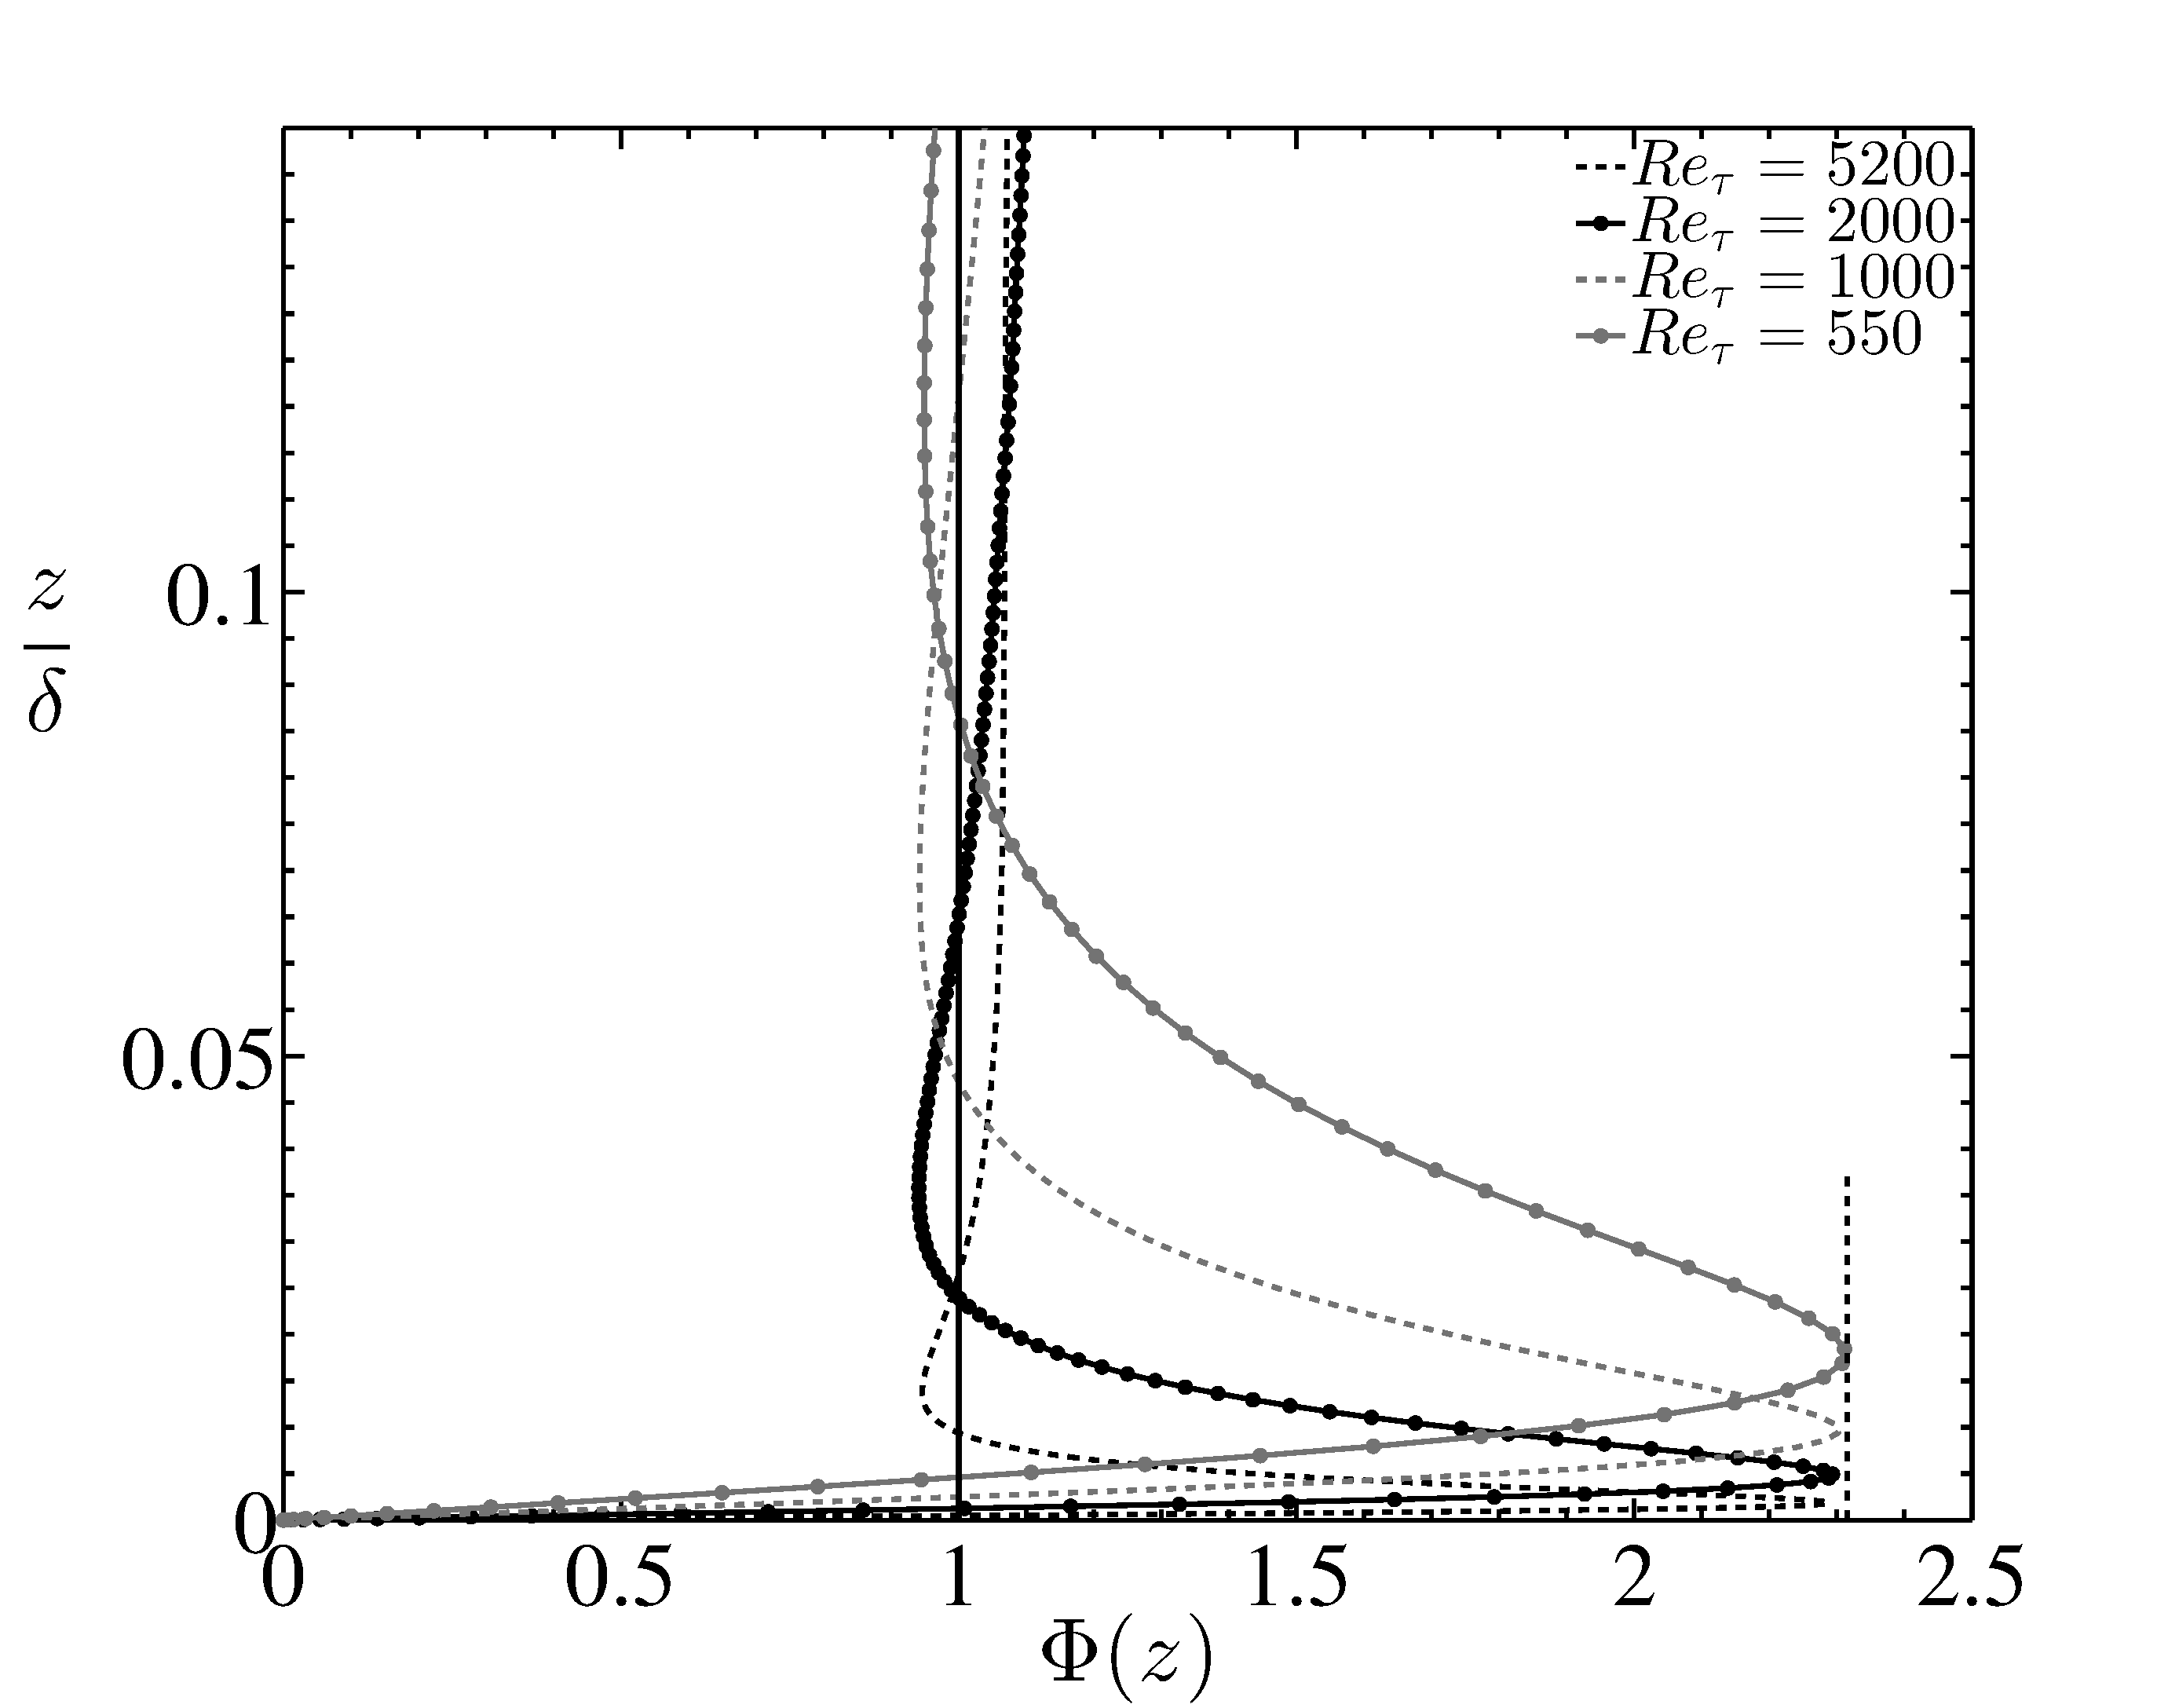
\includegraphics[width = \linewidth]{Figure/highRe2.pdf}
\end{subfigure}
\begin{subfigure}[t]{0.65\textwidth}
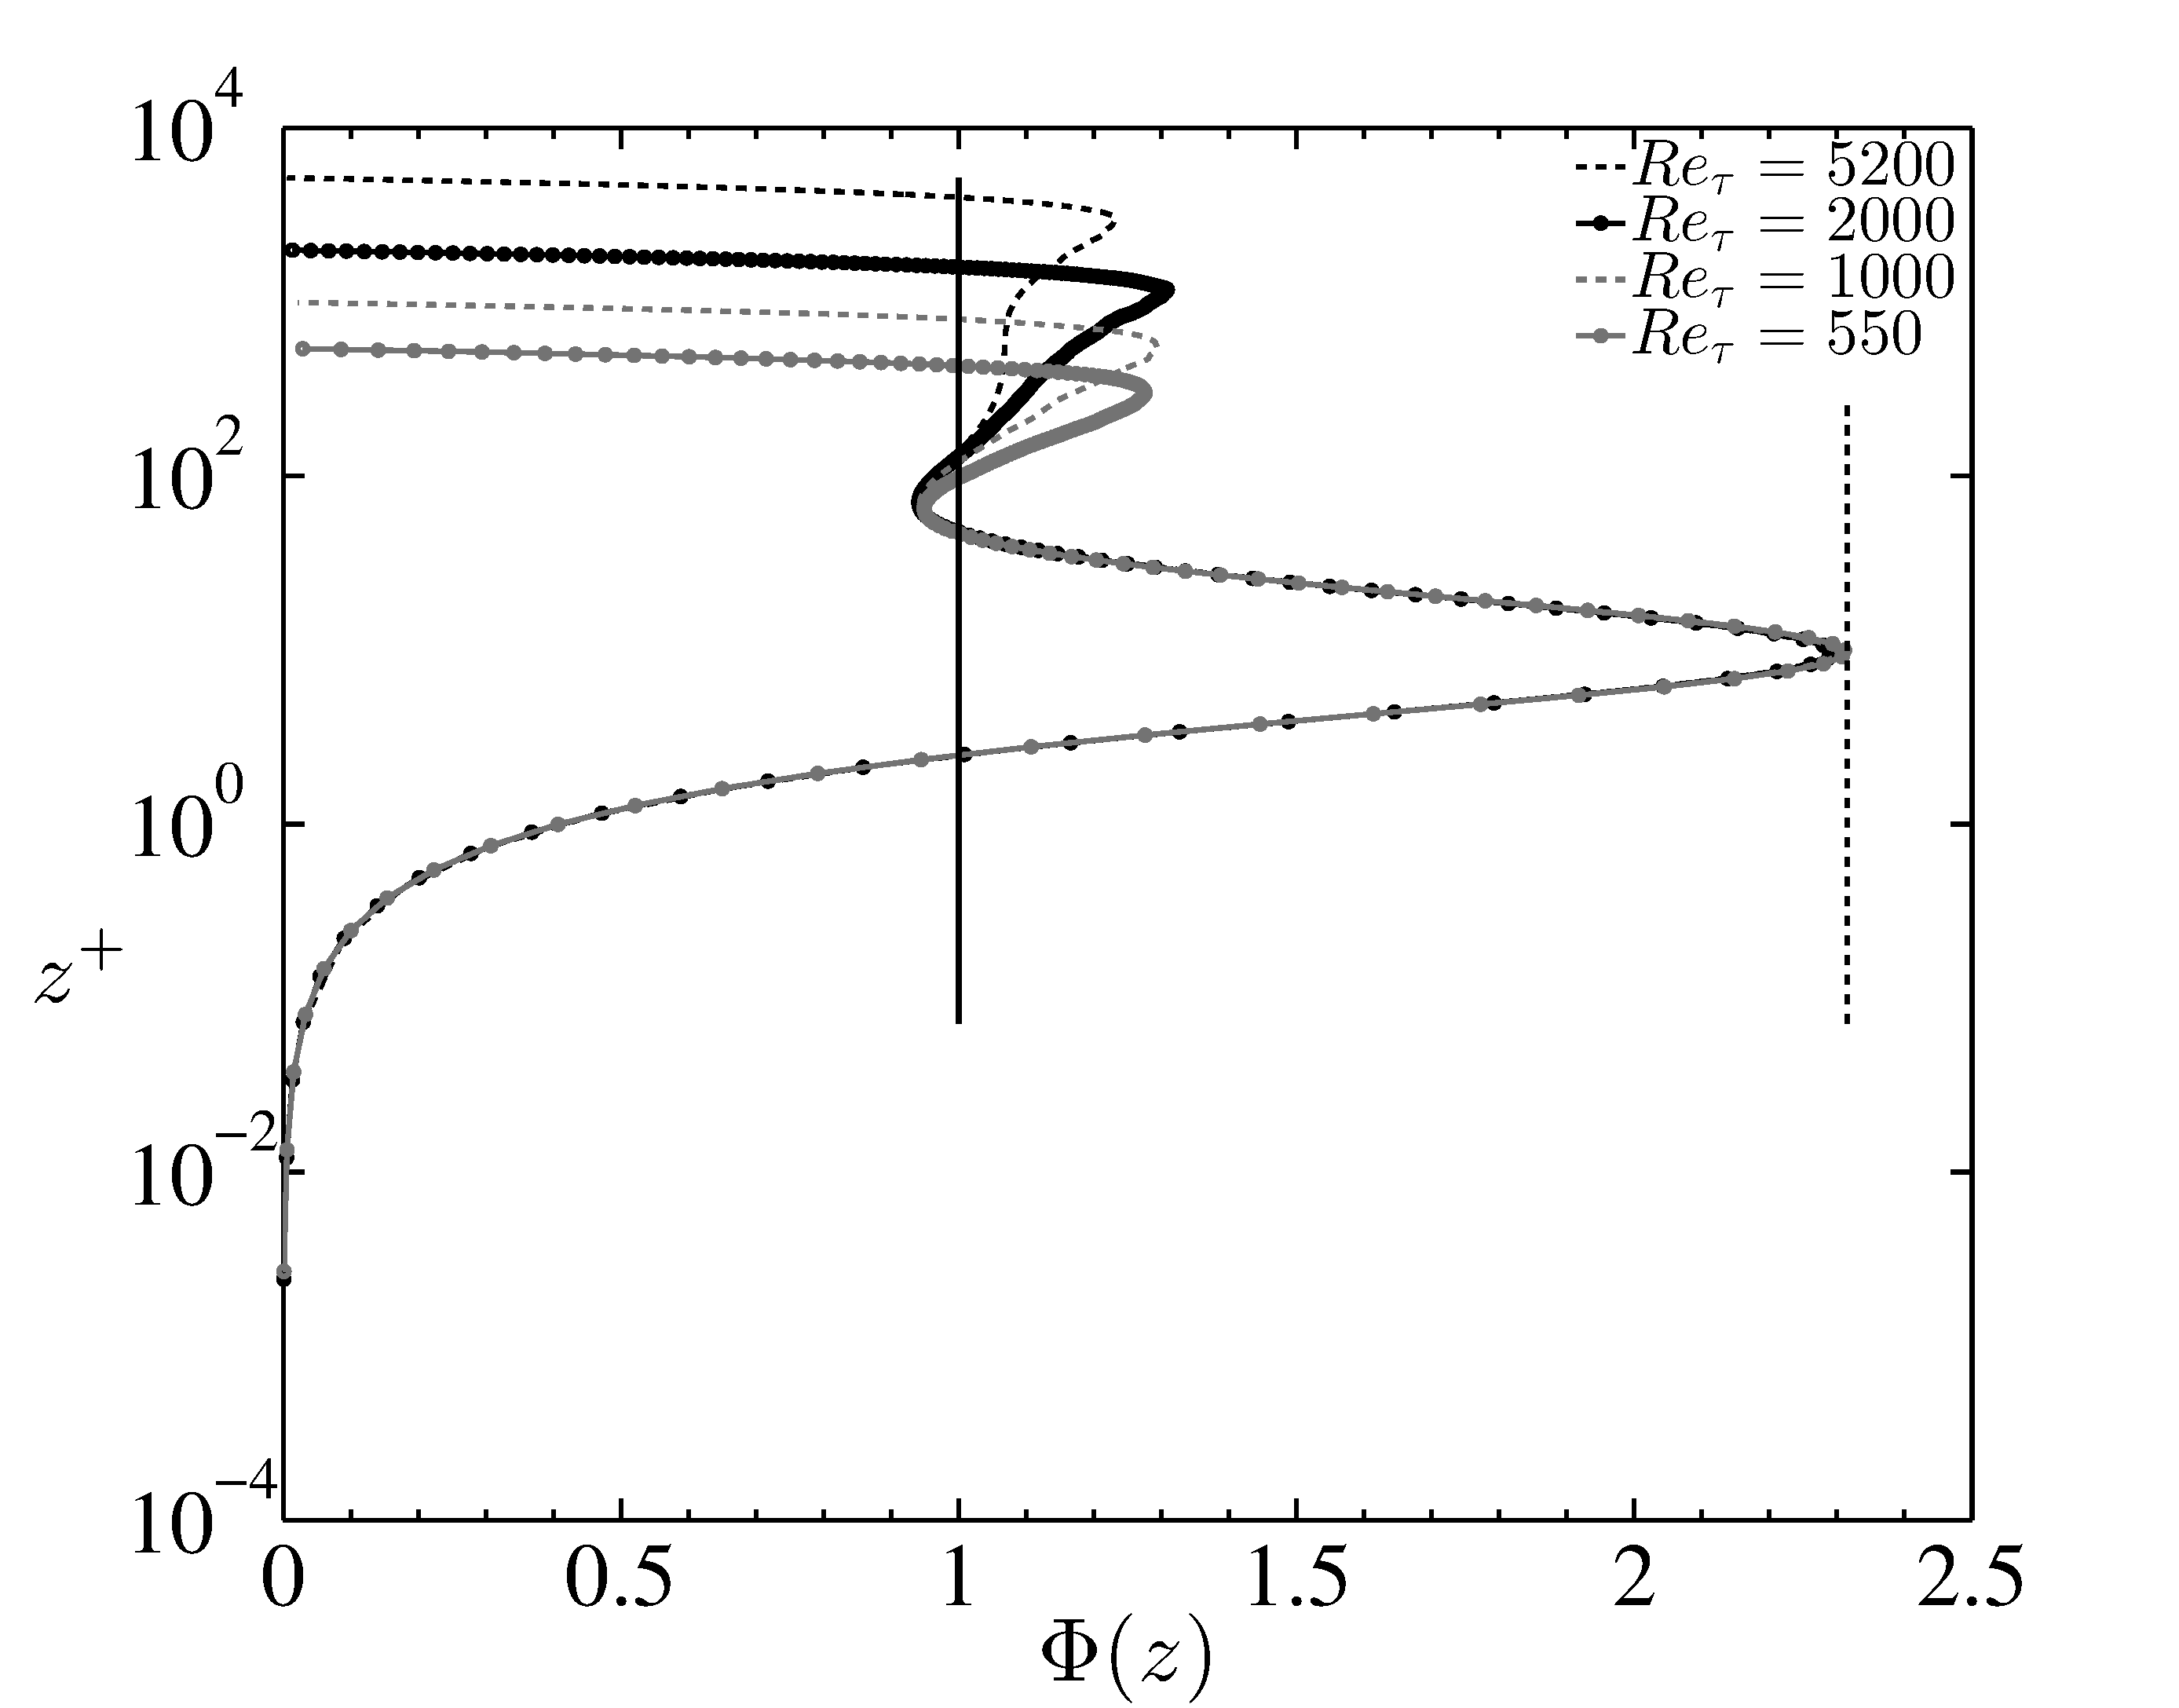
\includegraphics[width = \linewidth]{Figure/highRe2bb.pdf}
\end{subfigure}
\caption[Log-law deviation in high $Re_{\tau}$ channel flows]{High fidelity DNS simulations showing deviation of logarithmic trends $\Phi(z) \gg 1$ in the near-wall region, at very high Reynolds number channel flows.}\label{fig:hiRe}
\end{figure} 

\begin{figure}
\begin{minipage}{0.5\textwidth}
%\centering
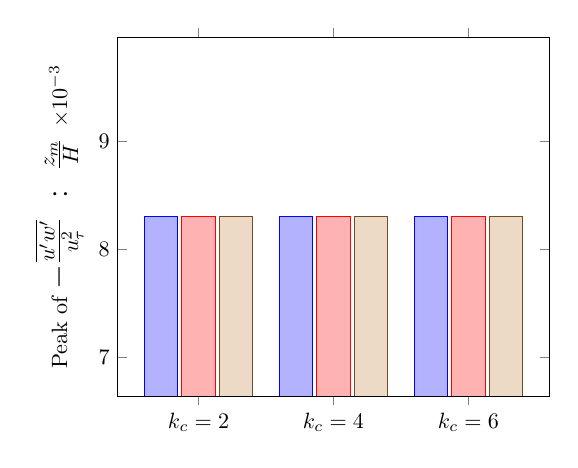
\begin{tikzpicture}[scale=0.8]
\begin{axis}[
    ybar,
    enlargelimits=0.3,
    legend style={at={(0.75,1.05)},
      anchor=north,legend columns=-1},
      ybar,
      bar width = 15pt,
    ylabel={Peak of \Large $-\frac{\overline{u'w'}}{u_{\tau}^2} \ : \ \frac{z_m}{H}$  \normalsize  $\times 10^{-3}$},
    symbolic x coords={$k_c=2$,$k_c=4$,$k_c=6$},
    xtick=data,
%    nodes near coords,
%    nodes near coords align={vertical},
    ]
\addplot coordinates {($k_c=2$,8.3) ($k_c=4$,8.3) ($k_c=6$,8.3)};
\addplot coordinates {($k_c=2$,8.3) ($k_c=4$,8.3) ($k_c=6$,8.3)};
\addplot coordinates {($k_c=2$,8.3) ($k_c=4$,8.3) ($k_c=6$,8.3)};
%\legend{I-IV,V-VII,VIII-X}
\end{axis}
\end{tikzpicture}
%\caption{Peak of normalized kinematic shear stress $-{uw_{rms}}/{u_{\tau}}^2$ in bar graph. Red: Cases I-IV $\lbrace C_0 = 0.16, n = 2 \rbrace$, Blue: Cases V-VII $\lbrace C_0 = 0.17, n = 1 \rbrace$ ,Green: Cases VIII-X $\lbrace C_0 = 0.19, n = \frac{1}{2} \rbrace$}\label{fig:bargraph}
%\captionof{figure}{Peak of normalized kinematic shear stress $-{uw_{rms}}/{u_{\tau}}^2$ in bar graph. Red: Cases I-IV $\lbrace C_0 = 0.16, n = 2 \rbrace$, Blue: Cases V-VII $\lbrace C_0 = 0.17, n = 1 \rbrace$ ,Green: Cases VIII-X $\lbrace C_0 = 0.19, n = \frac{1}{2} \rbrace$}
%\label{fig:fig2}
\end{minipage}%
\begin{minipage}{0.4\textwidth}
%\centering
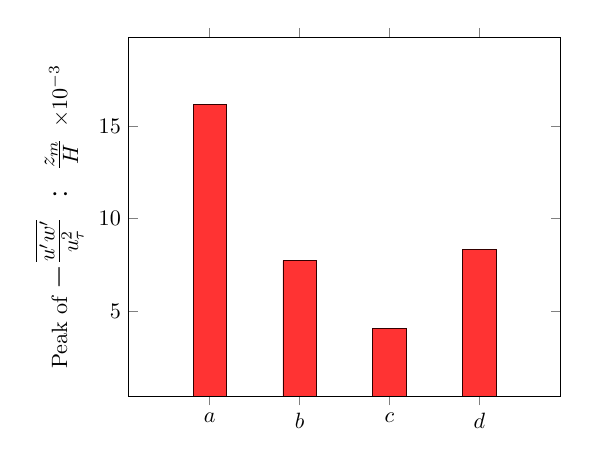
\begin{tikzpicture}[scale=0.8]
\begin{axis}[
    ybar,
    enlargelimits=0.3,
    legend style={at={(0.75,1.05)},
      anchor=north,legend columns=-1},
      ybar,
      bar width = 15pt,
    ylabel={Peak of \Large $-\frac{\overline{u'w'}}{u_{\tau}^2} \ : \ \frac{z_m}{H}$  \normalsize  $\times 10^{-3}$},
    symbolic x coords={$a$,$b$,$c$,$d$},
    xtick=data,
%    nodes near coords,
%    nodes near coords align={vertical},
    ]
\addplot[red!20!black,fill=red!80!white] coordinates {($a$,16.15) ($b$,7.72) ($c$,4.04) ($d$,8.33)};

%\legend{I-IV,V-VII,VIII-X}
\end{axis}
\end{tikzpicture}
%\caption{Peak of normalized kinematic shear stress $-{uw_{rms}}/{u_{\tau}}^2$ in bar graph. Red: Cases I-IV $\lbrace C_0 = 0.16, n = 2 \rbrace$, Blue: Cases V-VII $\lbrace C_0 = 0.17, n = 1 \rbrace$ ,Green: Cases VIII-X $\lbrace C_0 = 0.19, n = \frac{1}{2} \rbrace$}\label{fig:bargraph2}
%\captionof{figure}{Peak of normalized kinematic shear stress~\cite{porte1fun} (a) standard Smagorinsky (b) scale-dependant dynamic Smagorinsky (c) dynamic Smagorinsky }
%\label{fig:fig2}
\end{minipage}
\caption[Peak of kinematic shear stress]{\textit{Left}: Peak of normalized kinematic shear stress $-{uw_{rms}}/{u_{\tau}}^2$ in bar graph. Red: Cases I-IV $\lbrace C_0 = 0.16, n = 2 \rbrace$, Blue: Cases V-VII $\lbrace C_0 = 0.17, n = 1 \rbrace$ ,Green: Cases VIII-X $\lbrace C_0 = 0.19, n = \frac{1}{2} \rbrace$. \textit{Right}: Peak of normalized kinematic shear stress $-{uw_{rms}}/{u_{\tau}}^2$ ($a$,$b$,$c$) in Port\'{e}-Agel et. al~\cite{porte1fun}. $a$: standard Smagorinsky; $b$ scale-dependant dynamic Smagorinsky; $c$ dynamic Smagorinsky; $d$ current simulation with any set of $\lbrace C_0, \ n\rbrace$}\label{fig:peak}
\end{figure}

\begin{figure}
        \centering
        \begin{subfigure}[t]{0.5\textwidth}
                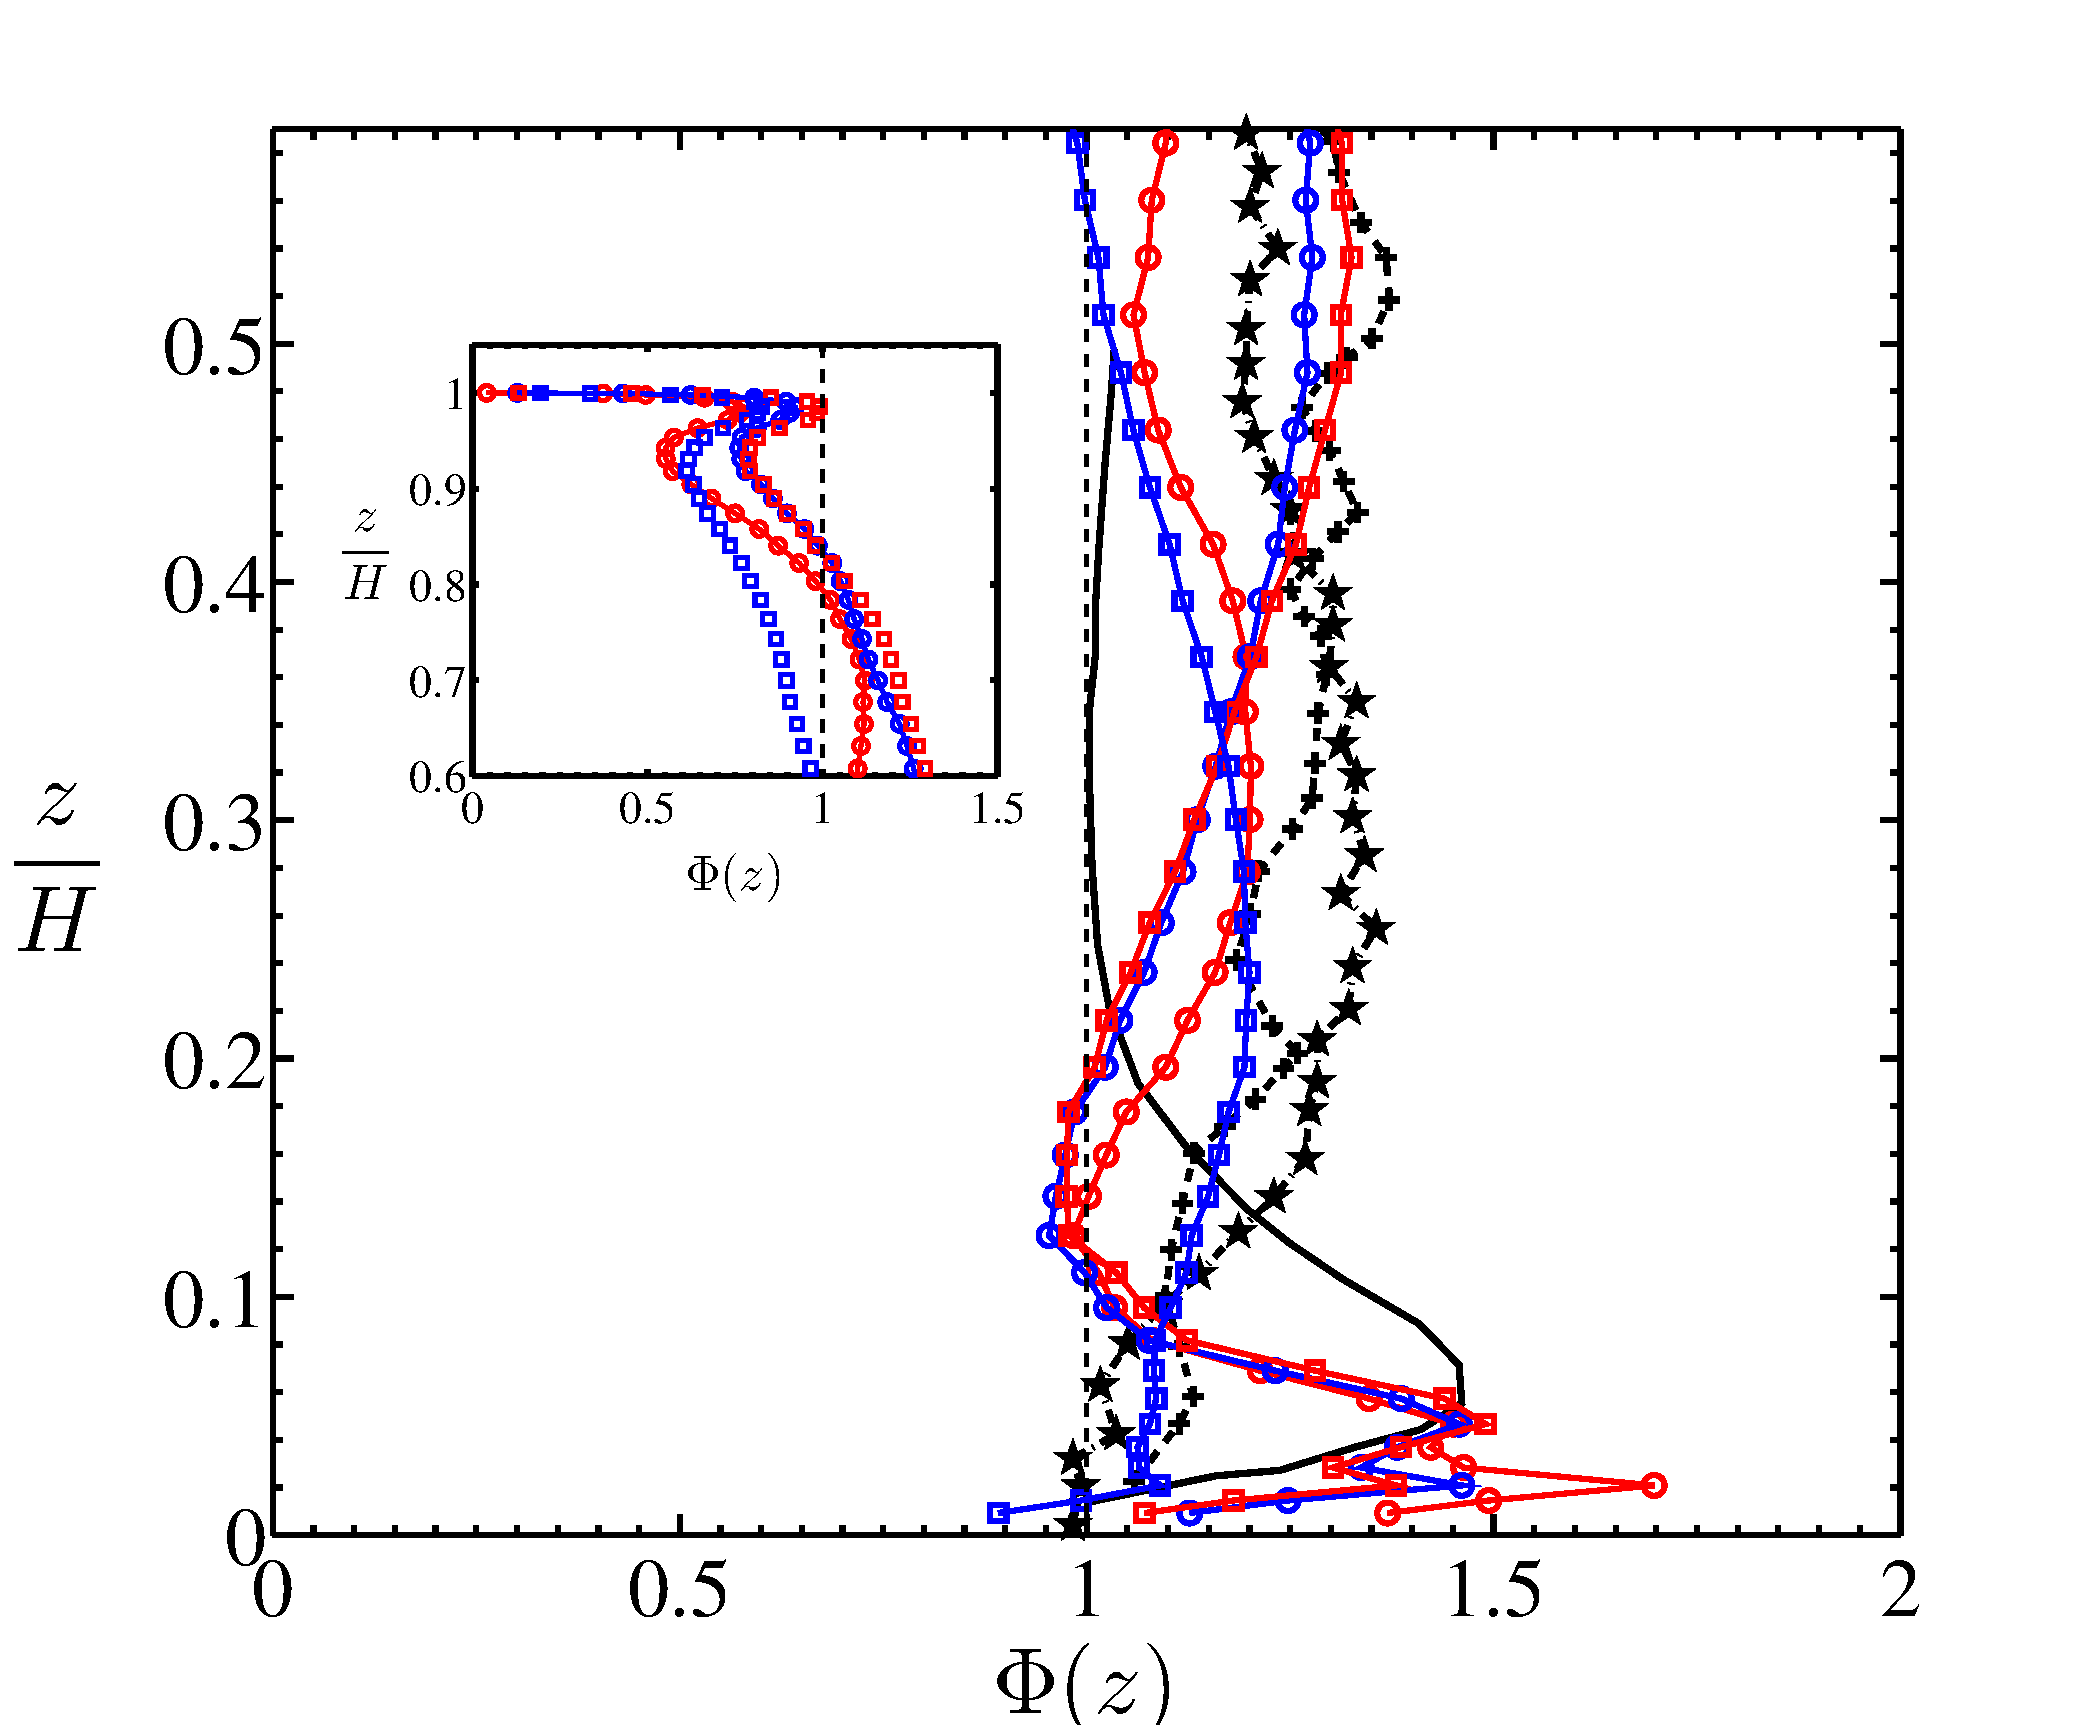
\includegraphics[width=\linewidth]{Fig2/gradient_filt_lotw.pdf}
                \caption{}
                \label{fig:grad1}
        \end{subfigure}%
        \centering
        \begin{subfigure}[t]{0.5\textwidth}
                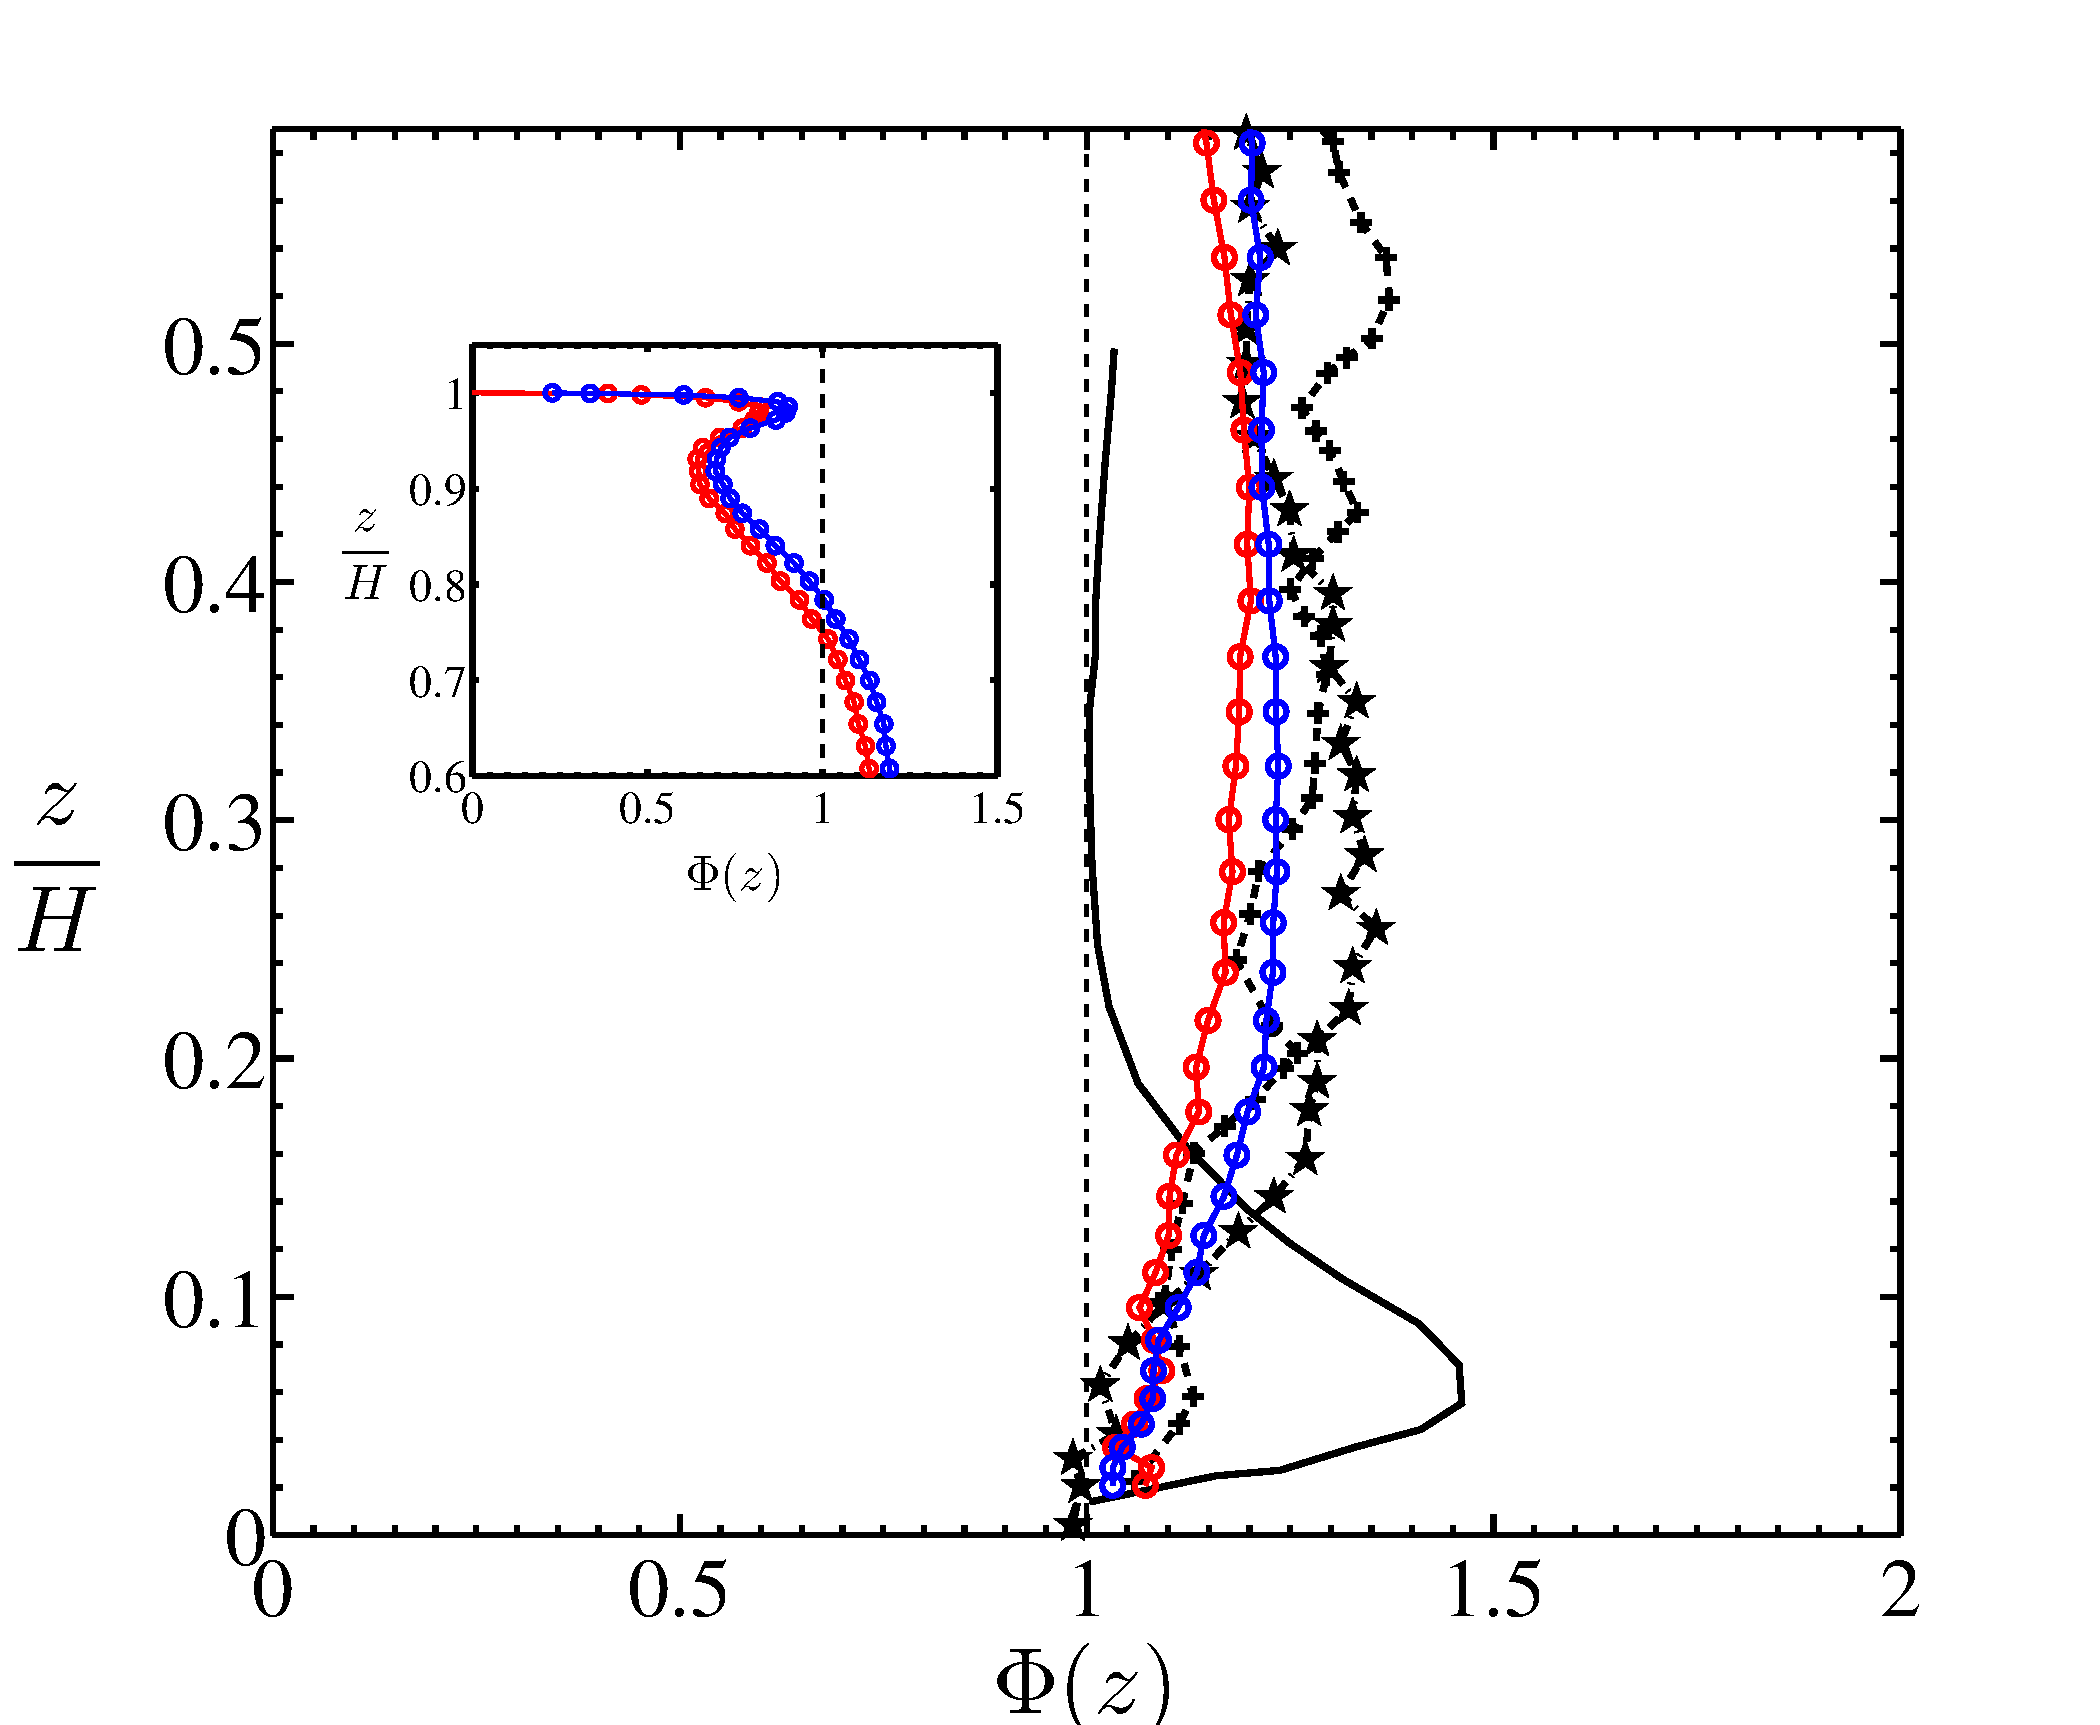
\includegraphics[width=\linewidth]{Fig2/gradient_filt_lotw2.pdf}
                \caption{}
                \label{fig:grad2}
        \end{subfigure}%
        \caption[$\Phi(z)$: interpolation, $C_0$]{Non dimensinonal mean streamwise velocity gradient $\phi(z)$ vs $z/H$. Red, Blue curves: current simulations; Black curves from the literature~\cite{porte1fun,bou1}. (a) $k_{c}=2$: Red $\circ$ $n = 1$; Blue $\circ$, $n = 2$; Red $\Box$, $n = 3$; Blue $\Box$, $C_0 = 0.13, n = \frac{1}{2}$.  (b) $k_c = 4$, $\lbrace C_0, \ n\rbrace = (0.19, 0.5)$: Red $\circ$ , spectral interpolation; Blue $\circ$ mid point interpolation. Black $+$ scale dependant dynamic Smagorinsky for Port$\acute{e}$-Agel et al.~\cite{porte1fun}; $-$ , standard Smagorinsky, $\star$, Lagrangian scale dependant dynamic Smagorinsky with filtering, Bou-Zeid et. al~\cite{bou1}}\label{fig:stat0_lotw}
\end{figure}

\begin{figure}
        \centering
        \begin{subfigure}[t]{0.55\textwidth}
                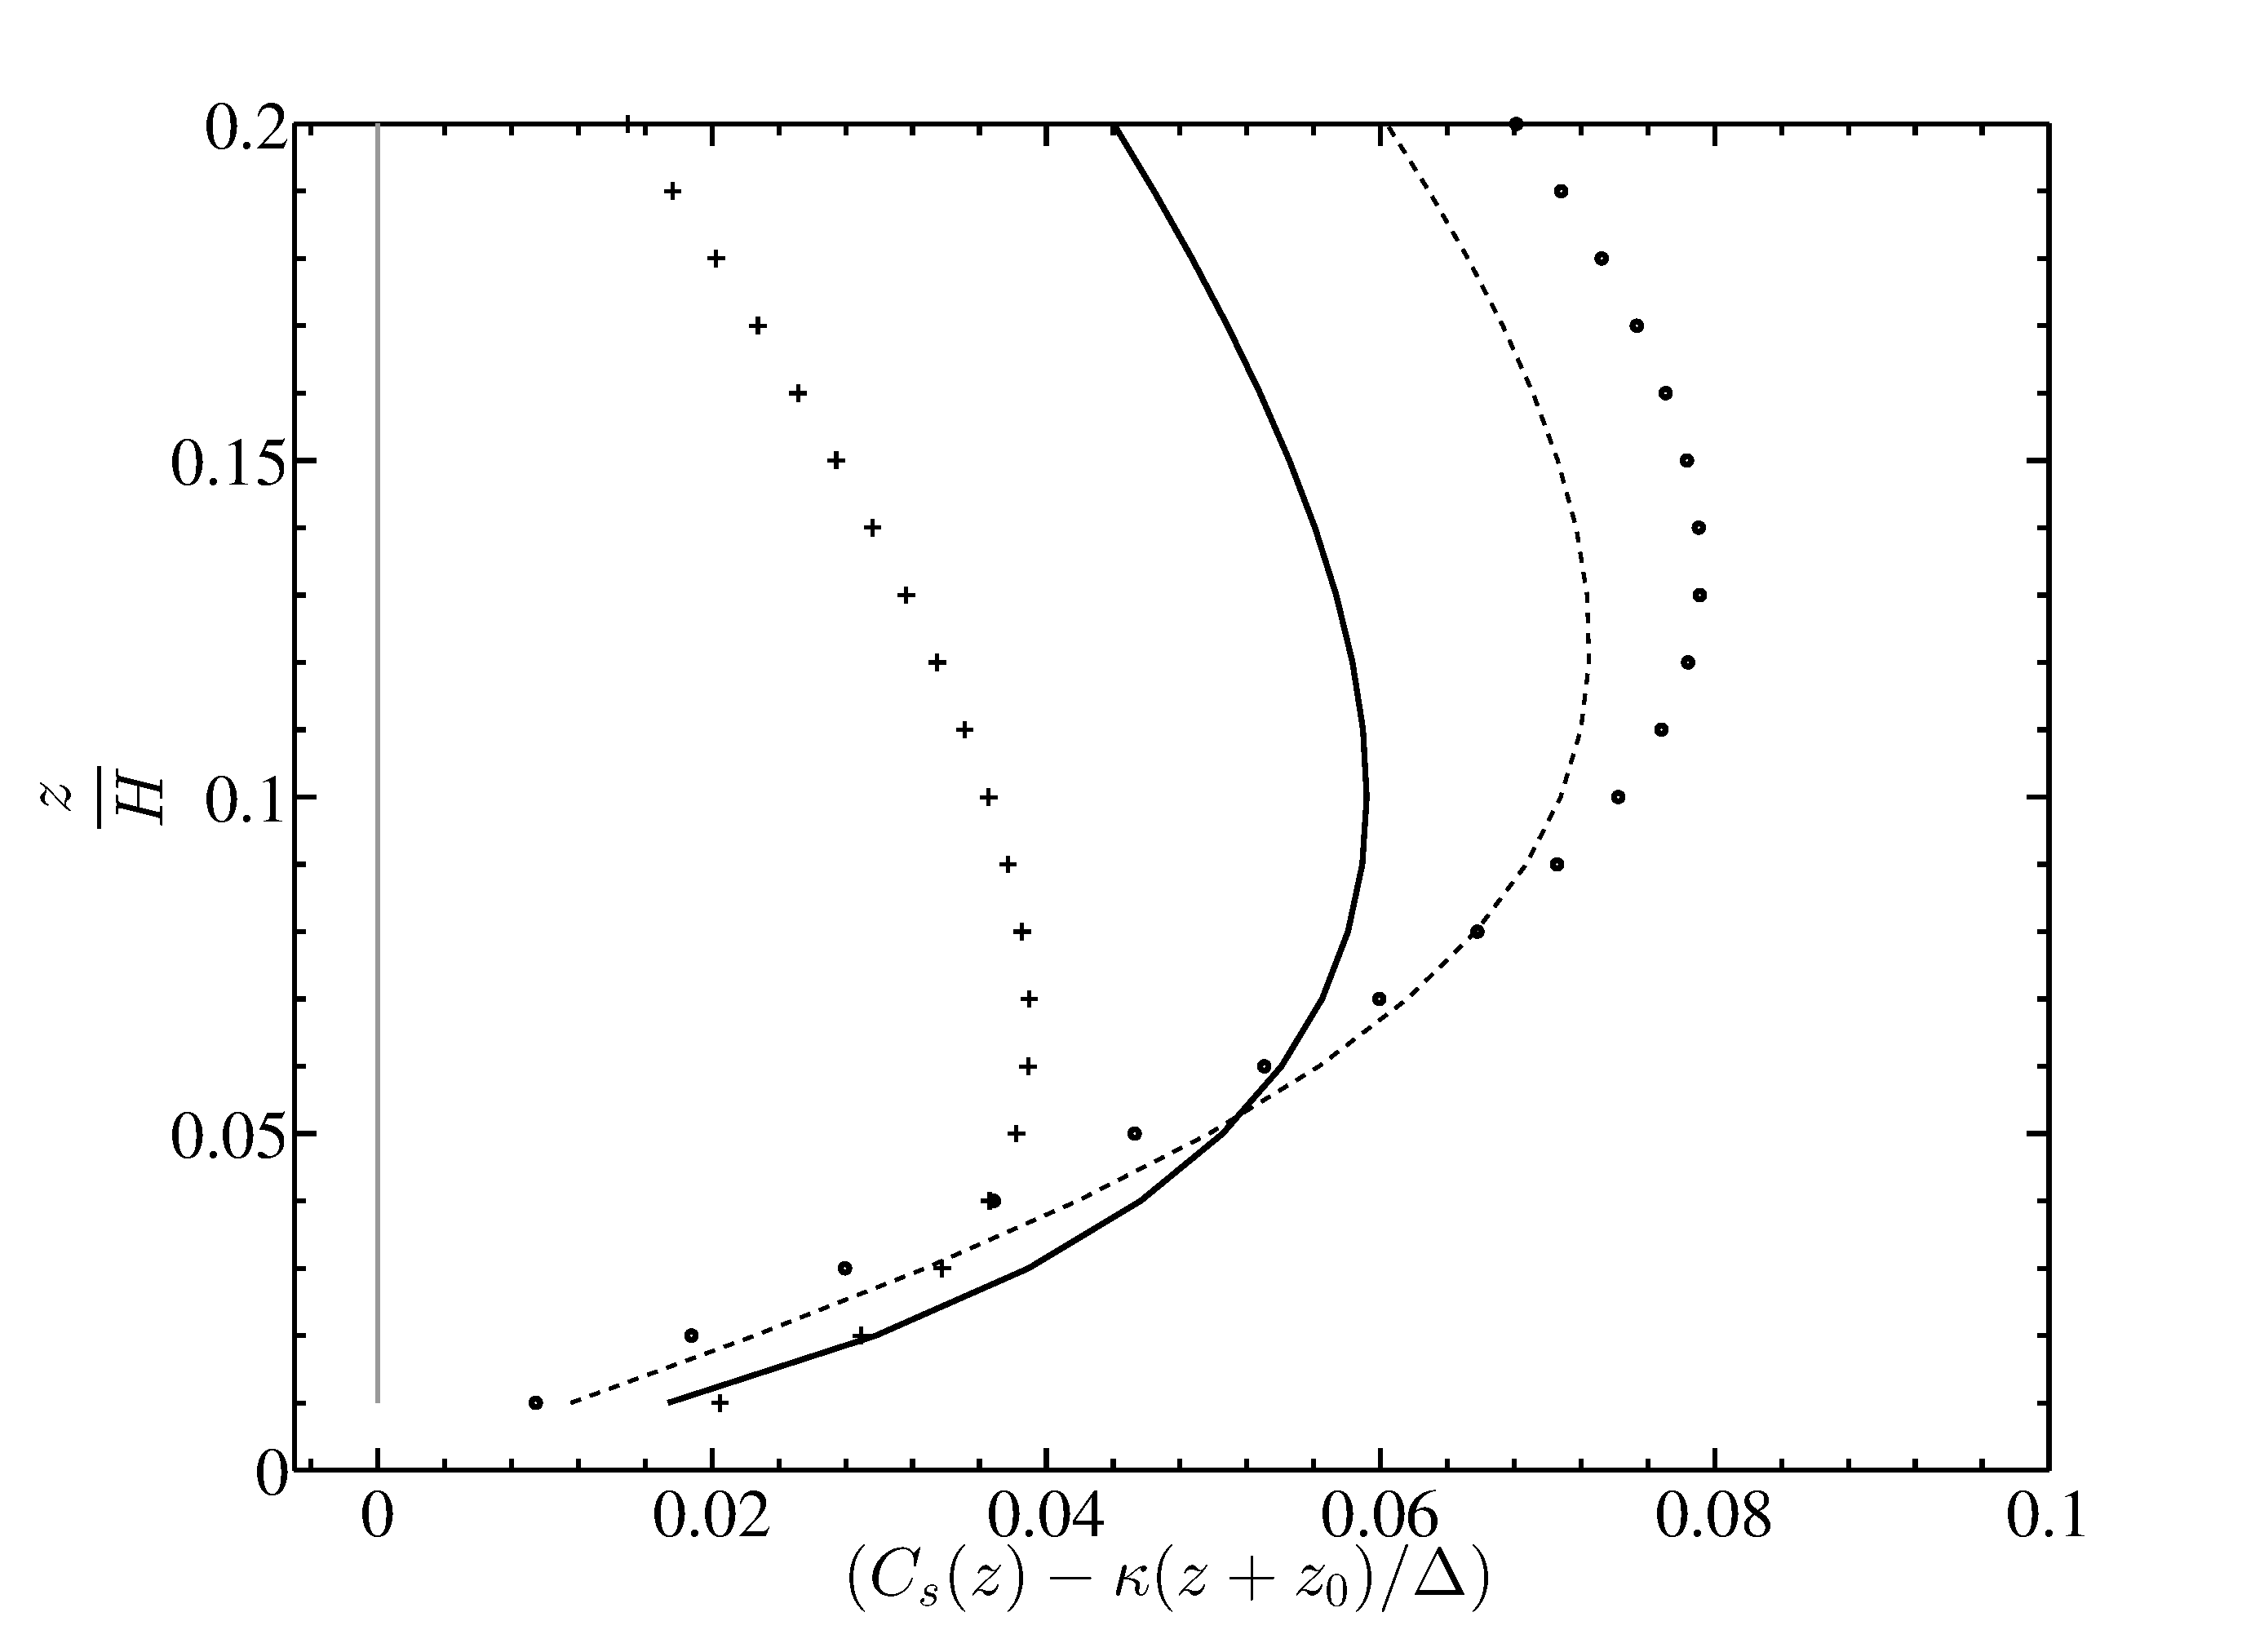
\includegraphics[width=\linewidth]{Fig2/Smag2b_abs.pdf}
                \caption{}
                \label{fig:error1}
        \end{subfigure}%
        \centering
        \begin{subfigure}[t]{0.45\textwidth}
                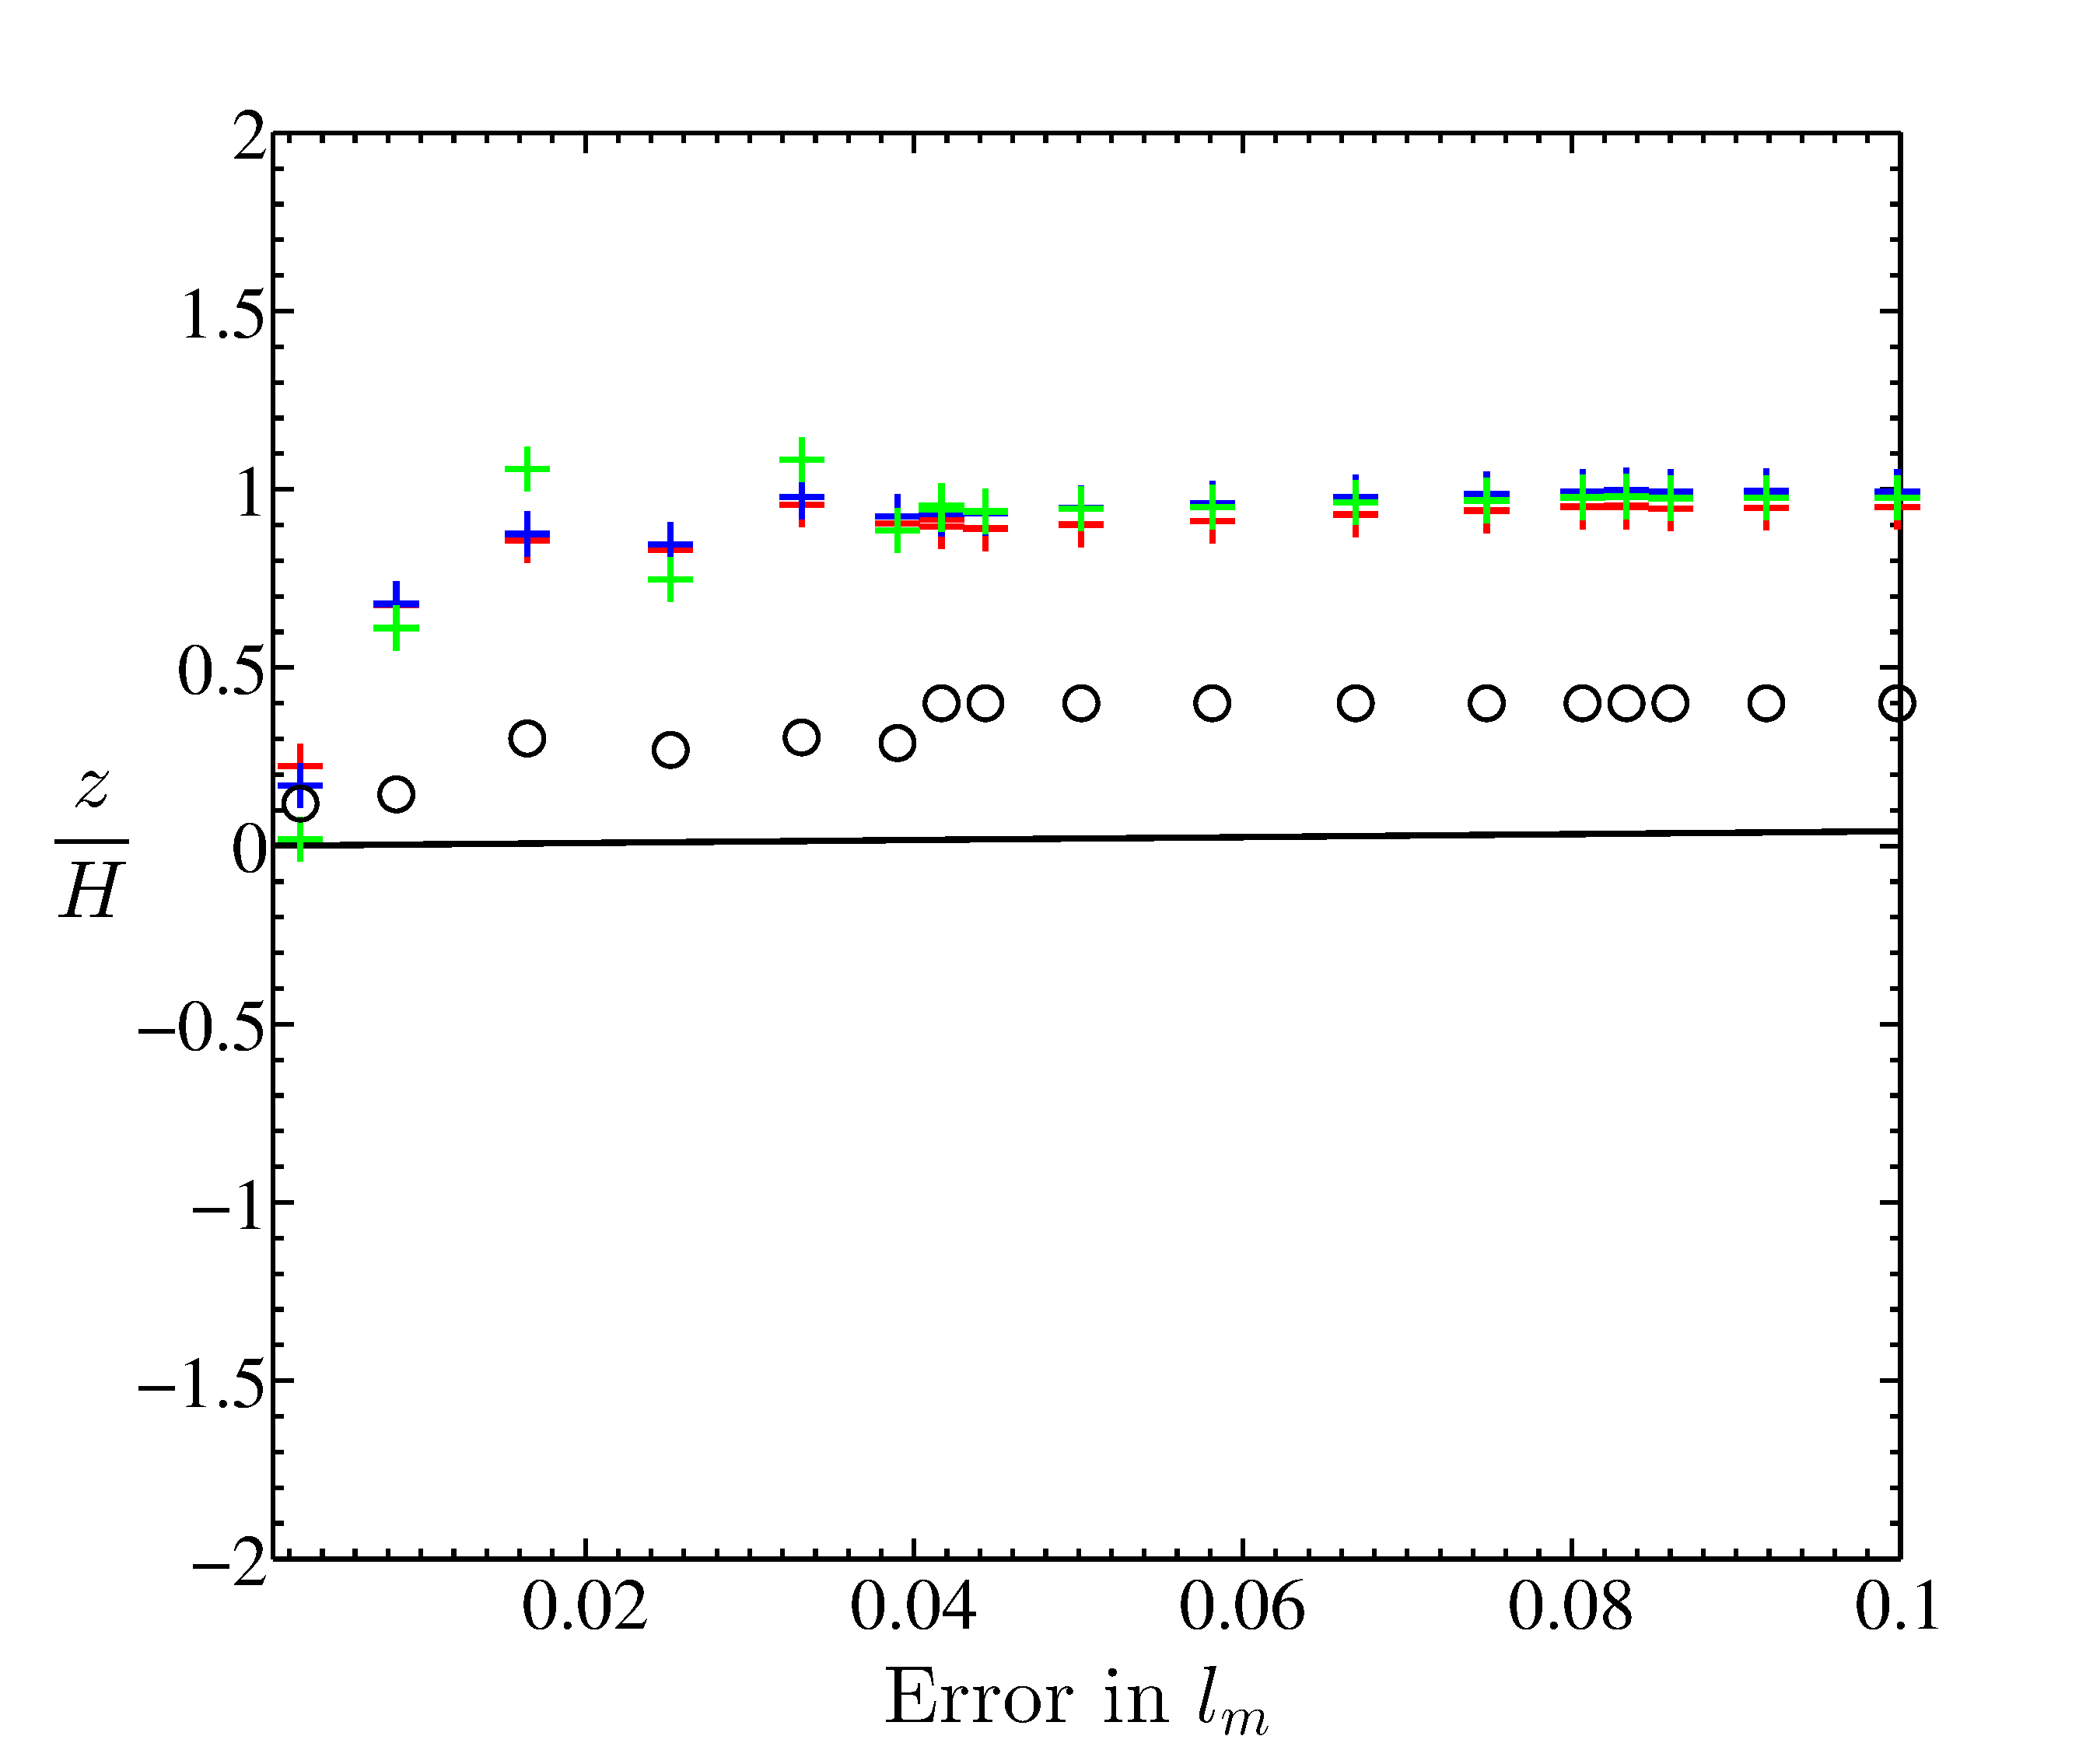
\includegraphics[width=\linewidth]{Fig2/shear_filter_n123.pdf}
                \caption{}
                \label{fig:error2}
        \end{subfigure}
\caption[Errors contributing in log-layer mismatch]{(a)Error $E_{1}$ in filter-scale $l_f$ compared to mixing length scale at log-layer $\kappa z$. (b) Error $E2$ in eddy-turnover time length scale $u_{\tau} \times t_{eddy}$ compared to log-layer mixing-length scale $\kappa z$. solid Black line: $\kappa z$. Symbols: Red, Blue $\&$ Green $+$, corresponds to $(n = 1, C_0 = 0.17, k_c = 4)$, $(n = 1, C_0 = 0.17,k_c = 2)$, $(n = 1, C_0 = 0.13, k_c = 4)$ respectively. Black $\circ$, $(n = \frac{1}{2}, C_0 = 0.19, k_c = 4)$. $E_1$ is the modelling error, $E_2$ is the numerical error.}
                \label{fig:shear1}
\end{figure}

\begin{figure}[h!]
        \centering
        \begin{subfigure}[t]{0.70\textwidth}
                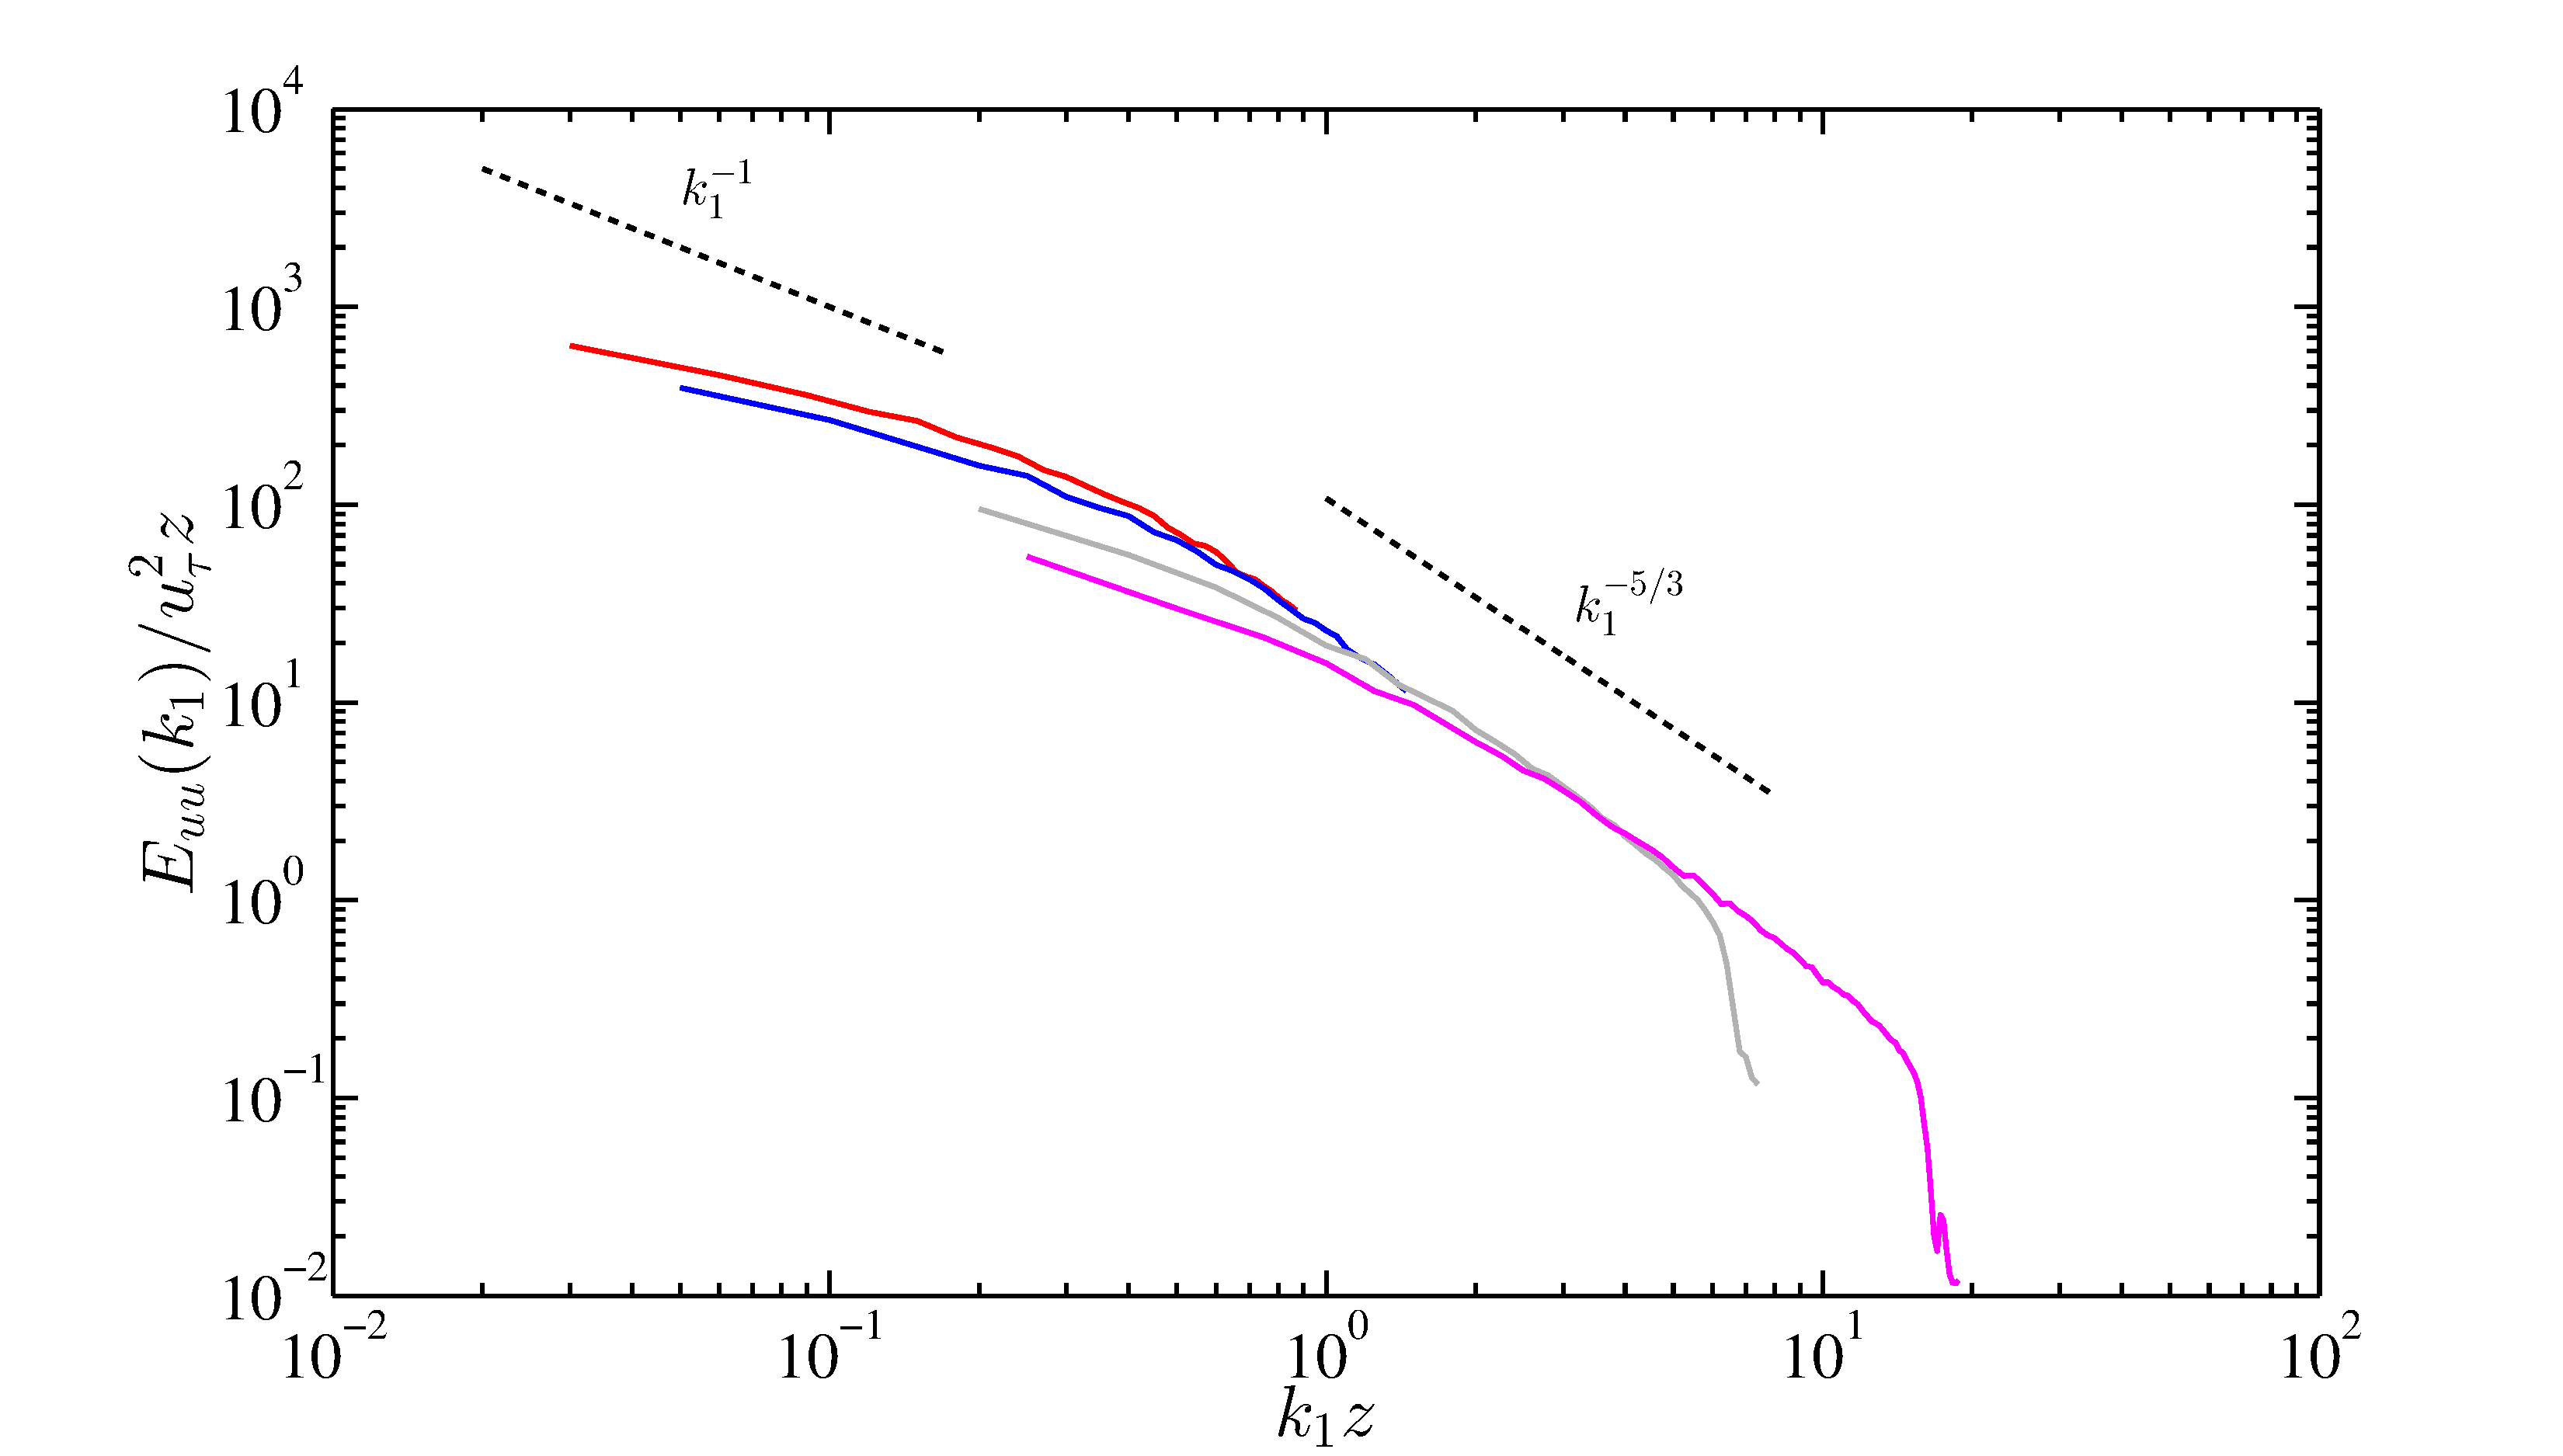
\includegraphics[width=\linewidth]{Fig2/energy_ABL_n05_filt2.pdf}
                \caption{}
                \label{fig:spec}
        \end{subfigure}
\centering
        \begin{subfigure}[t]{0.70\textwidth}
                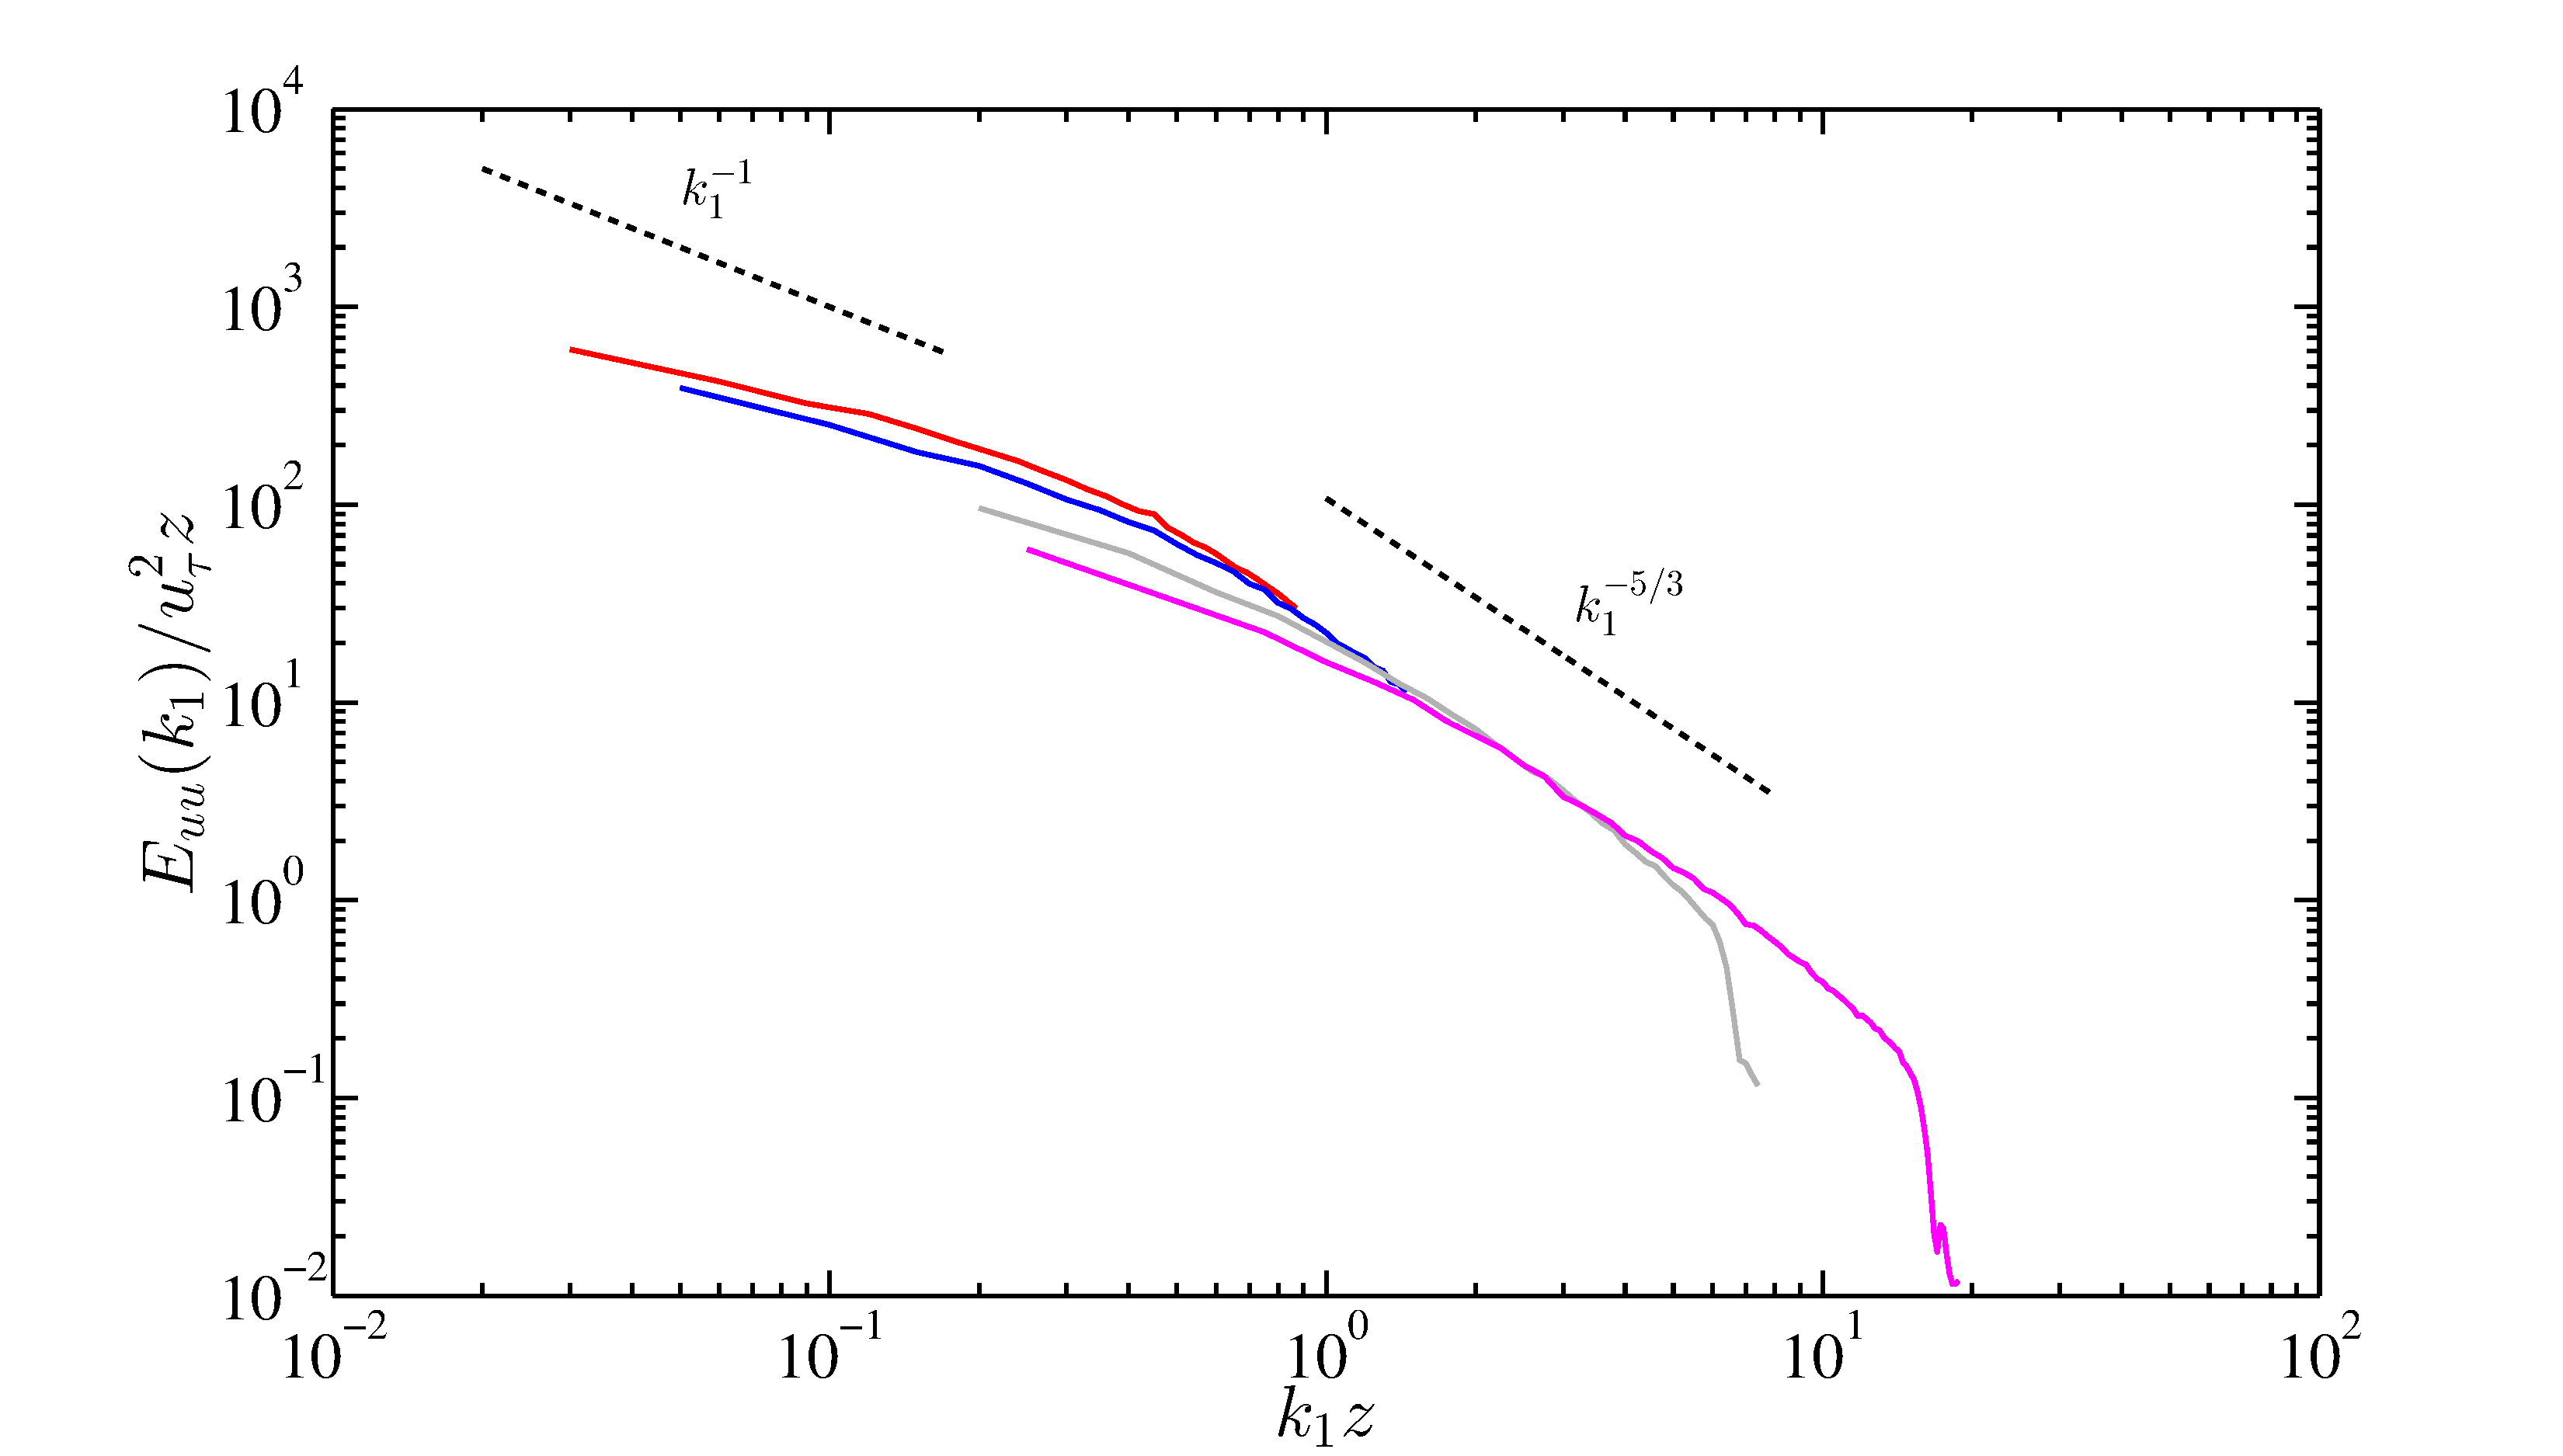
\includegraphics[width=\linewidth]{Fig2/energy_ABL_n05_filt4.pdf}
                \caption{}
                \label{fig:spec2}
        \end{subfigure}
\centering
        \begin{subfigure}[t]{0.70\textwidth}
                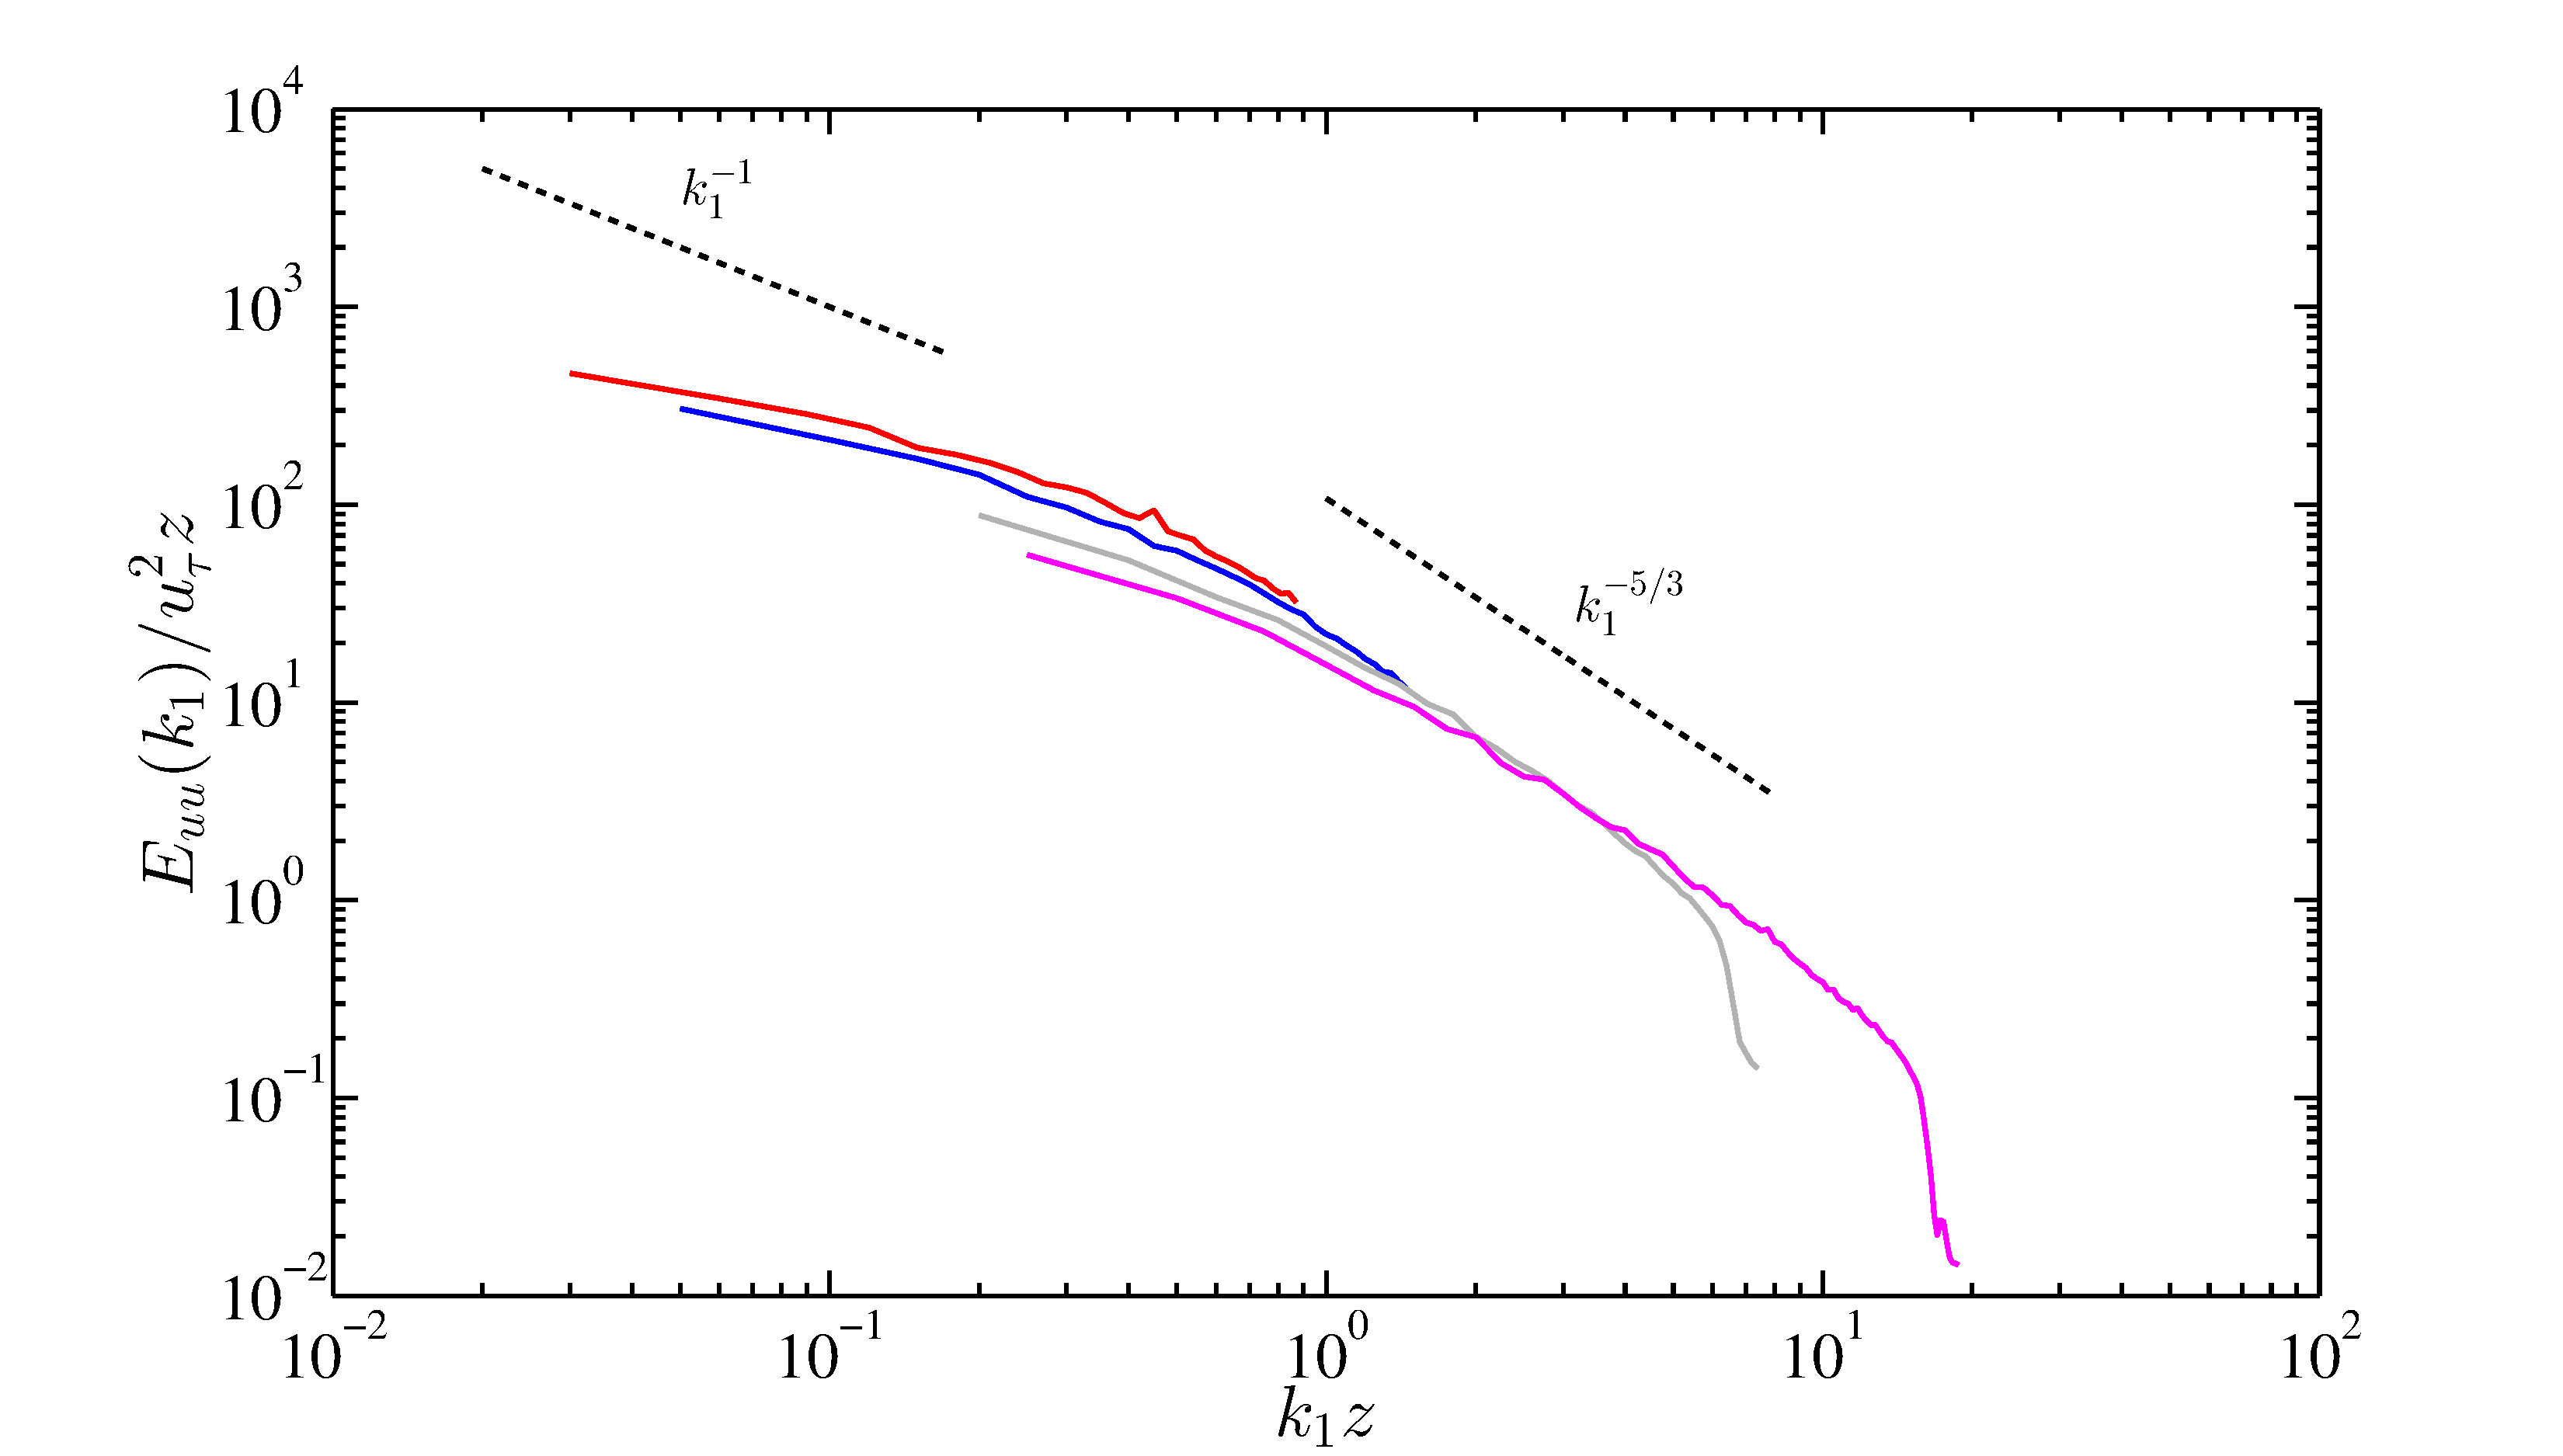
\includegraphics[width=\linewidth]{Fig2/energy_ABL_n05_filt6.pdf}
                \caption{}
                \label{fig:spec3}
        \end{subfigure}        
        \caption[1D Energy Spectra 1]{ Temporally and Horizontally averaged streamwise energy spectrum (A) Case VII, $k_c = 2$ (B) Case VIII, $k_c = 4$ (C) Case IX, $k_c = 6$. The Smagorinsky mixing length damping parameters $\lbrace C_0, \ n \rbrace = \lbrace 0.19, 0.5\rbrace$ are fixed, $k_c$ is varied. $k_1$ is the streamwise wavenumber. Red, $z/H = 0.015$, Blue, $z/H = 0.025$, Grey, $z/H = 0.1$, Magenta, $z/H = 0.25$ }\label{fig:stat0_lotw2}
\end{figure}
        
   \begin{figure}        
\centering
          \begin{subfigure}[t]{0.70\textwidth}
                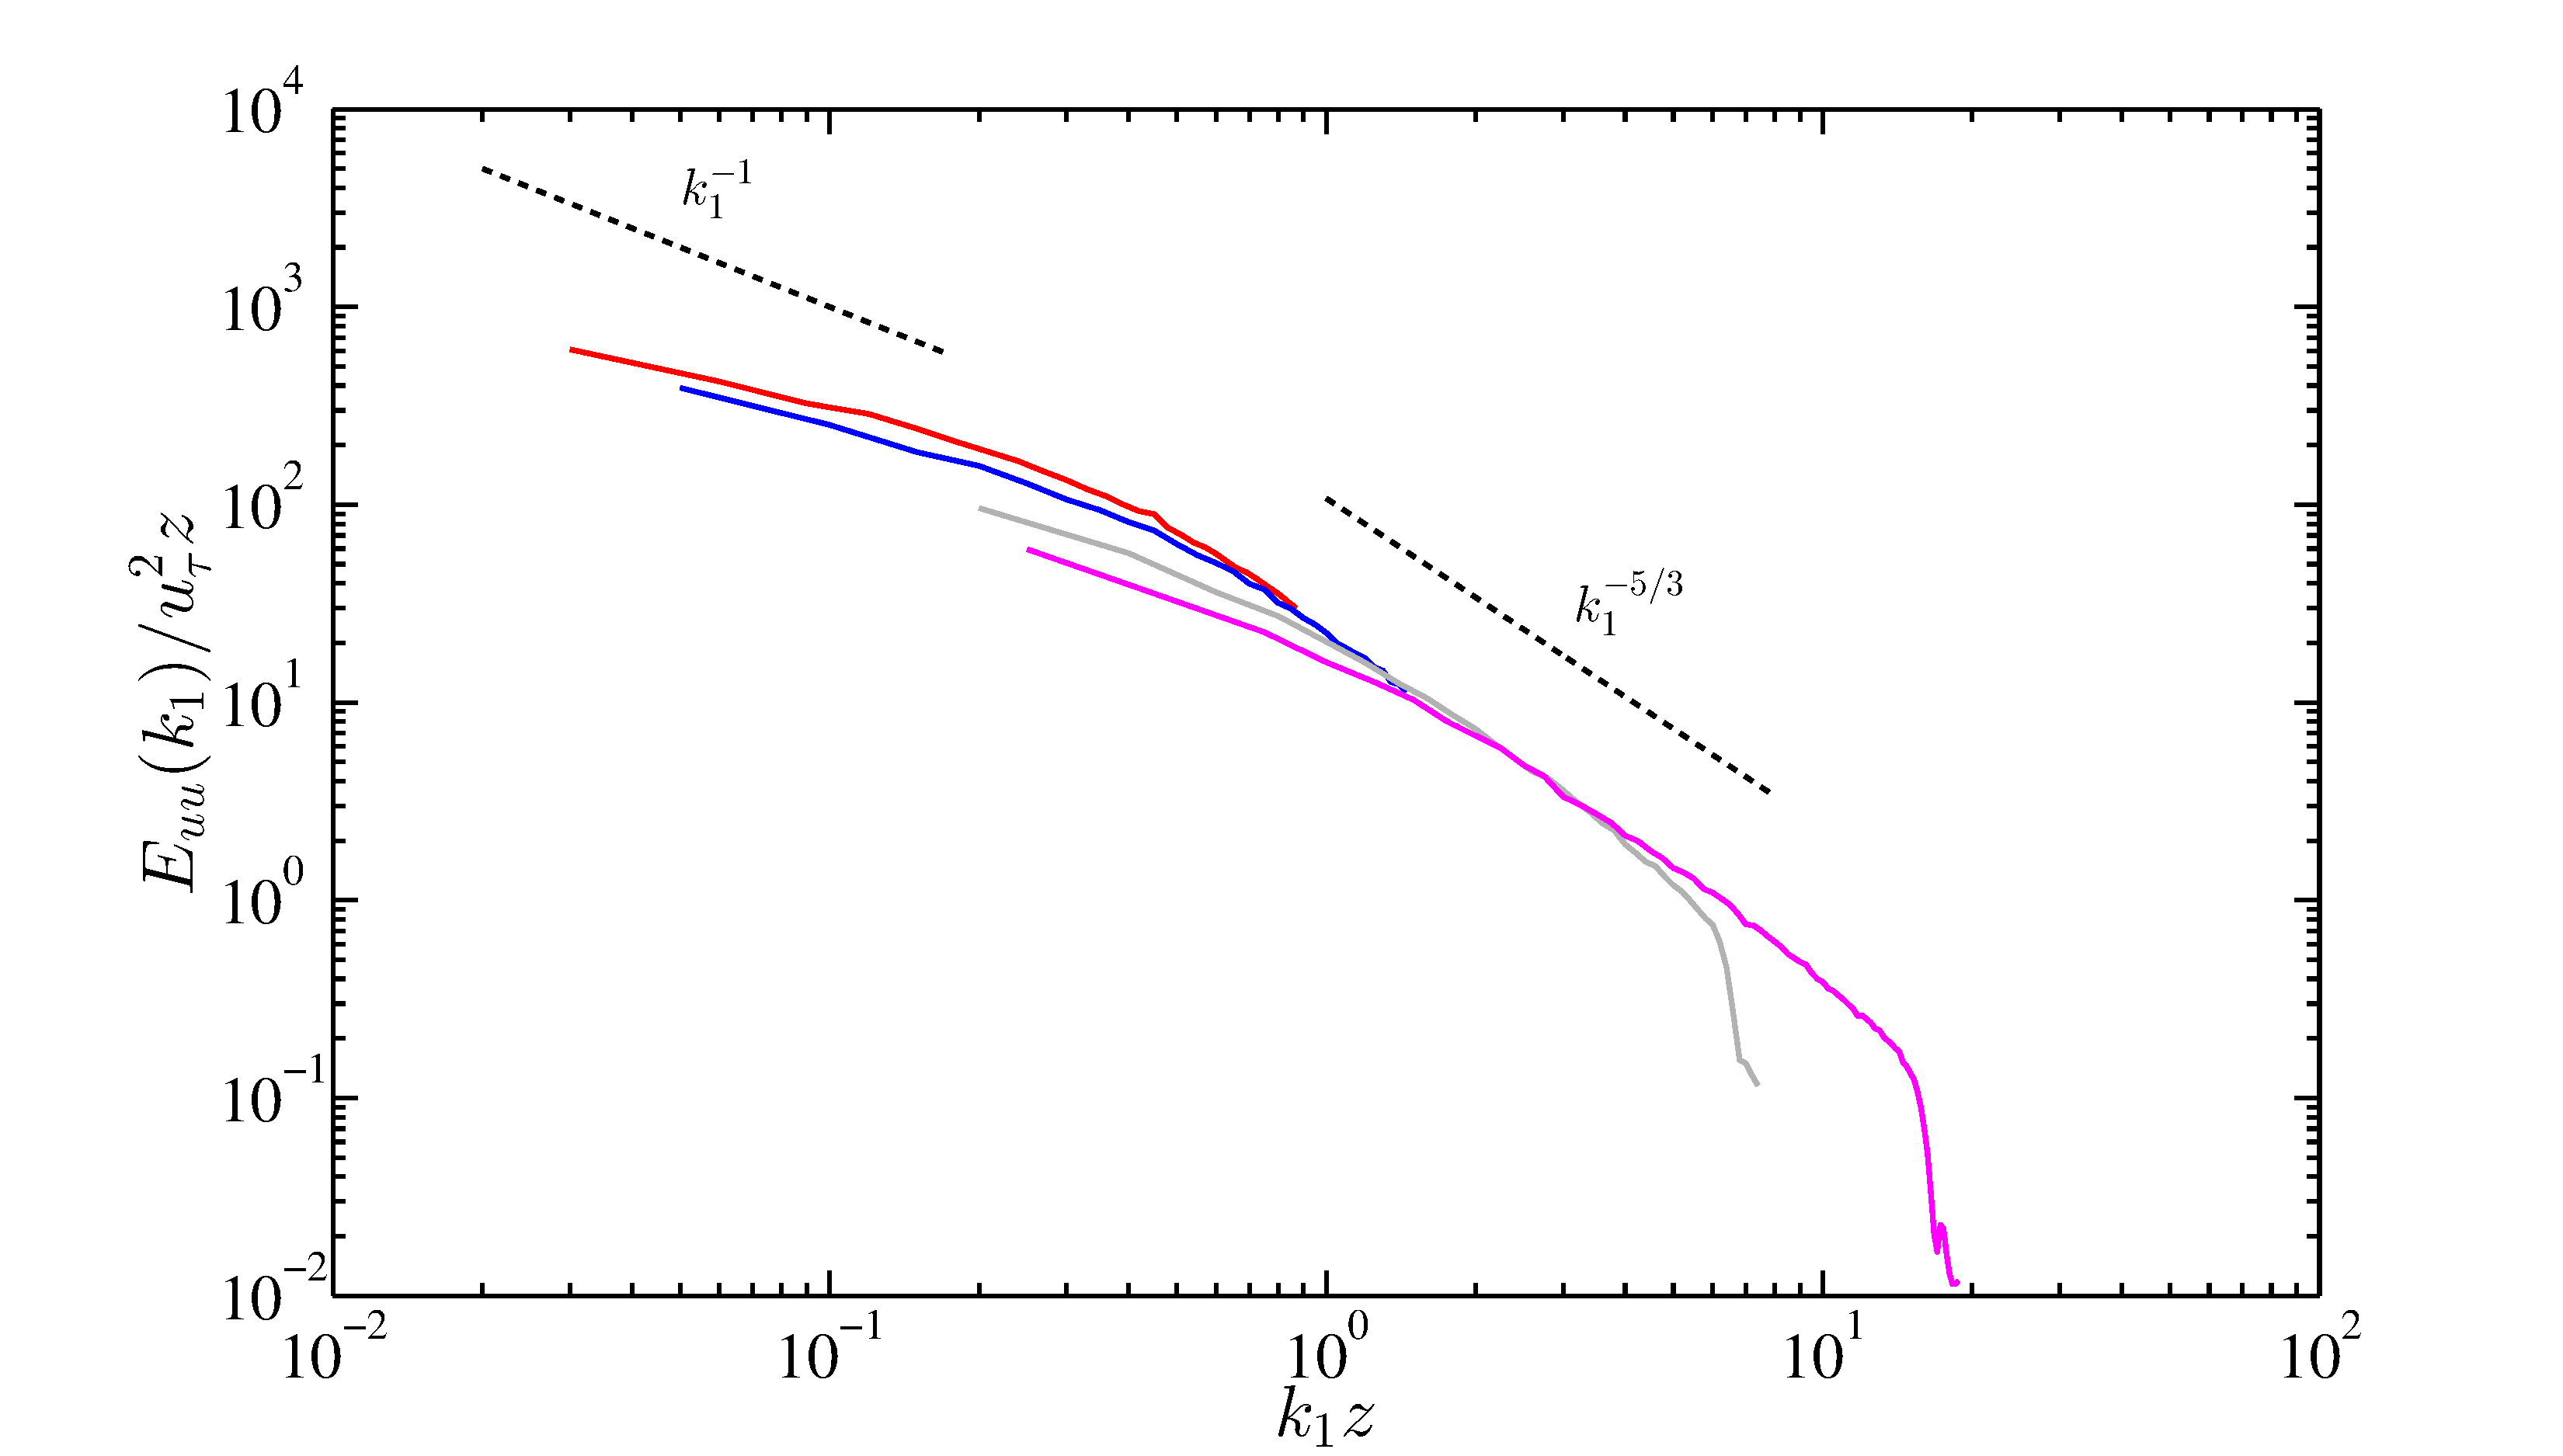
\includegraphics[width=\linewidth]{Fig2/energy_ABL_n05_filt4.pdf}
                \caption{}
                \label{fig:spec4}
        \end{subfigure}   
\centering
          \begin{subfigure}[t]{0.70\textwidth}
                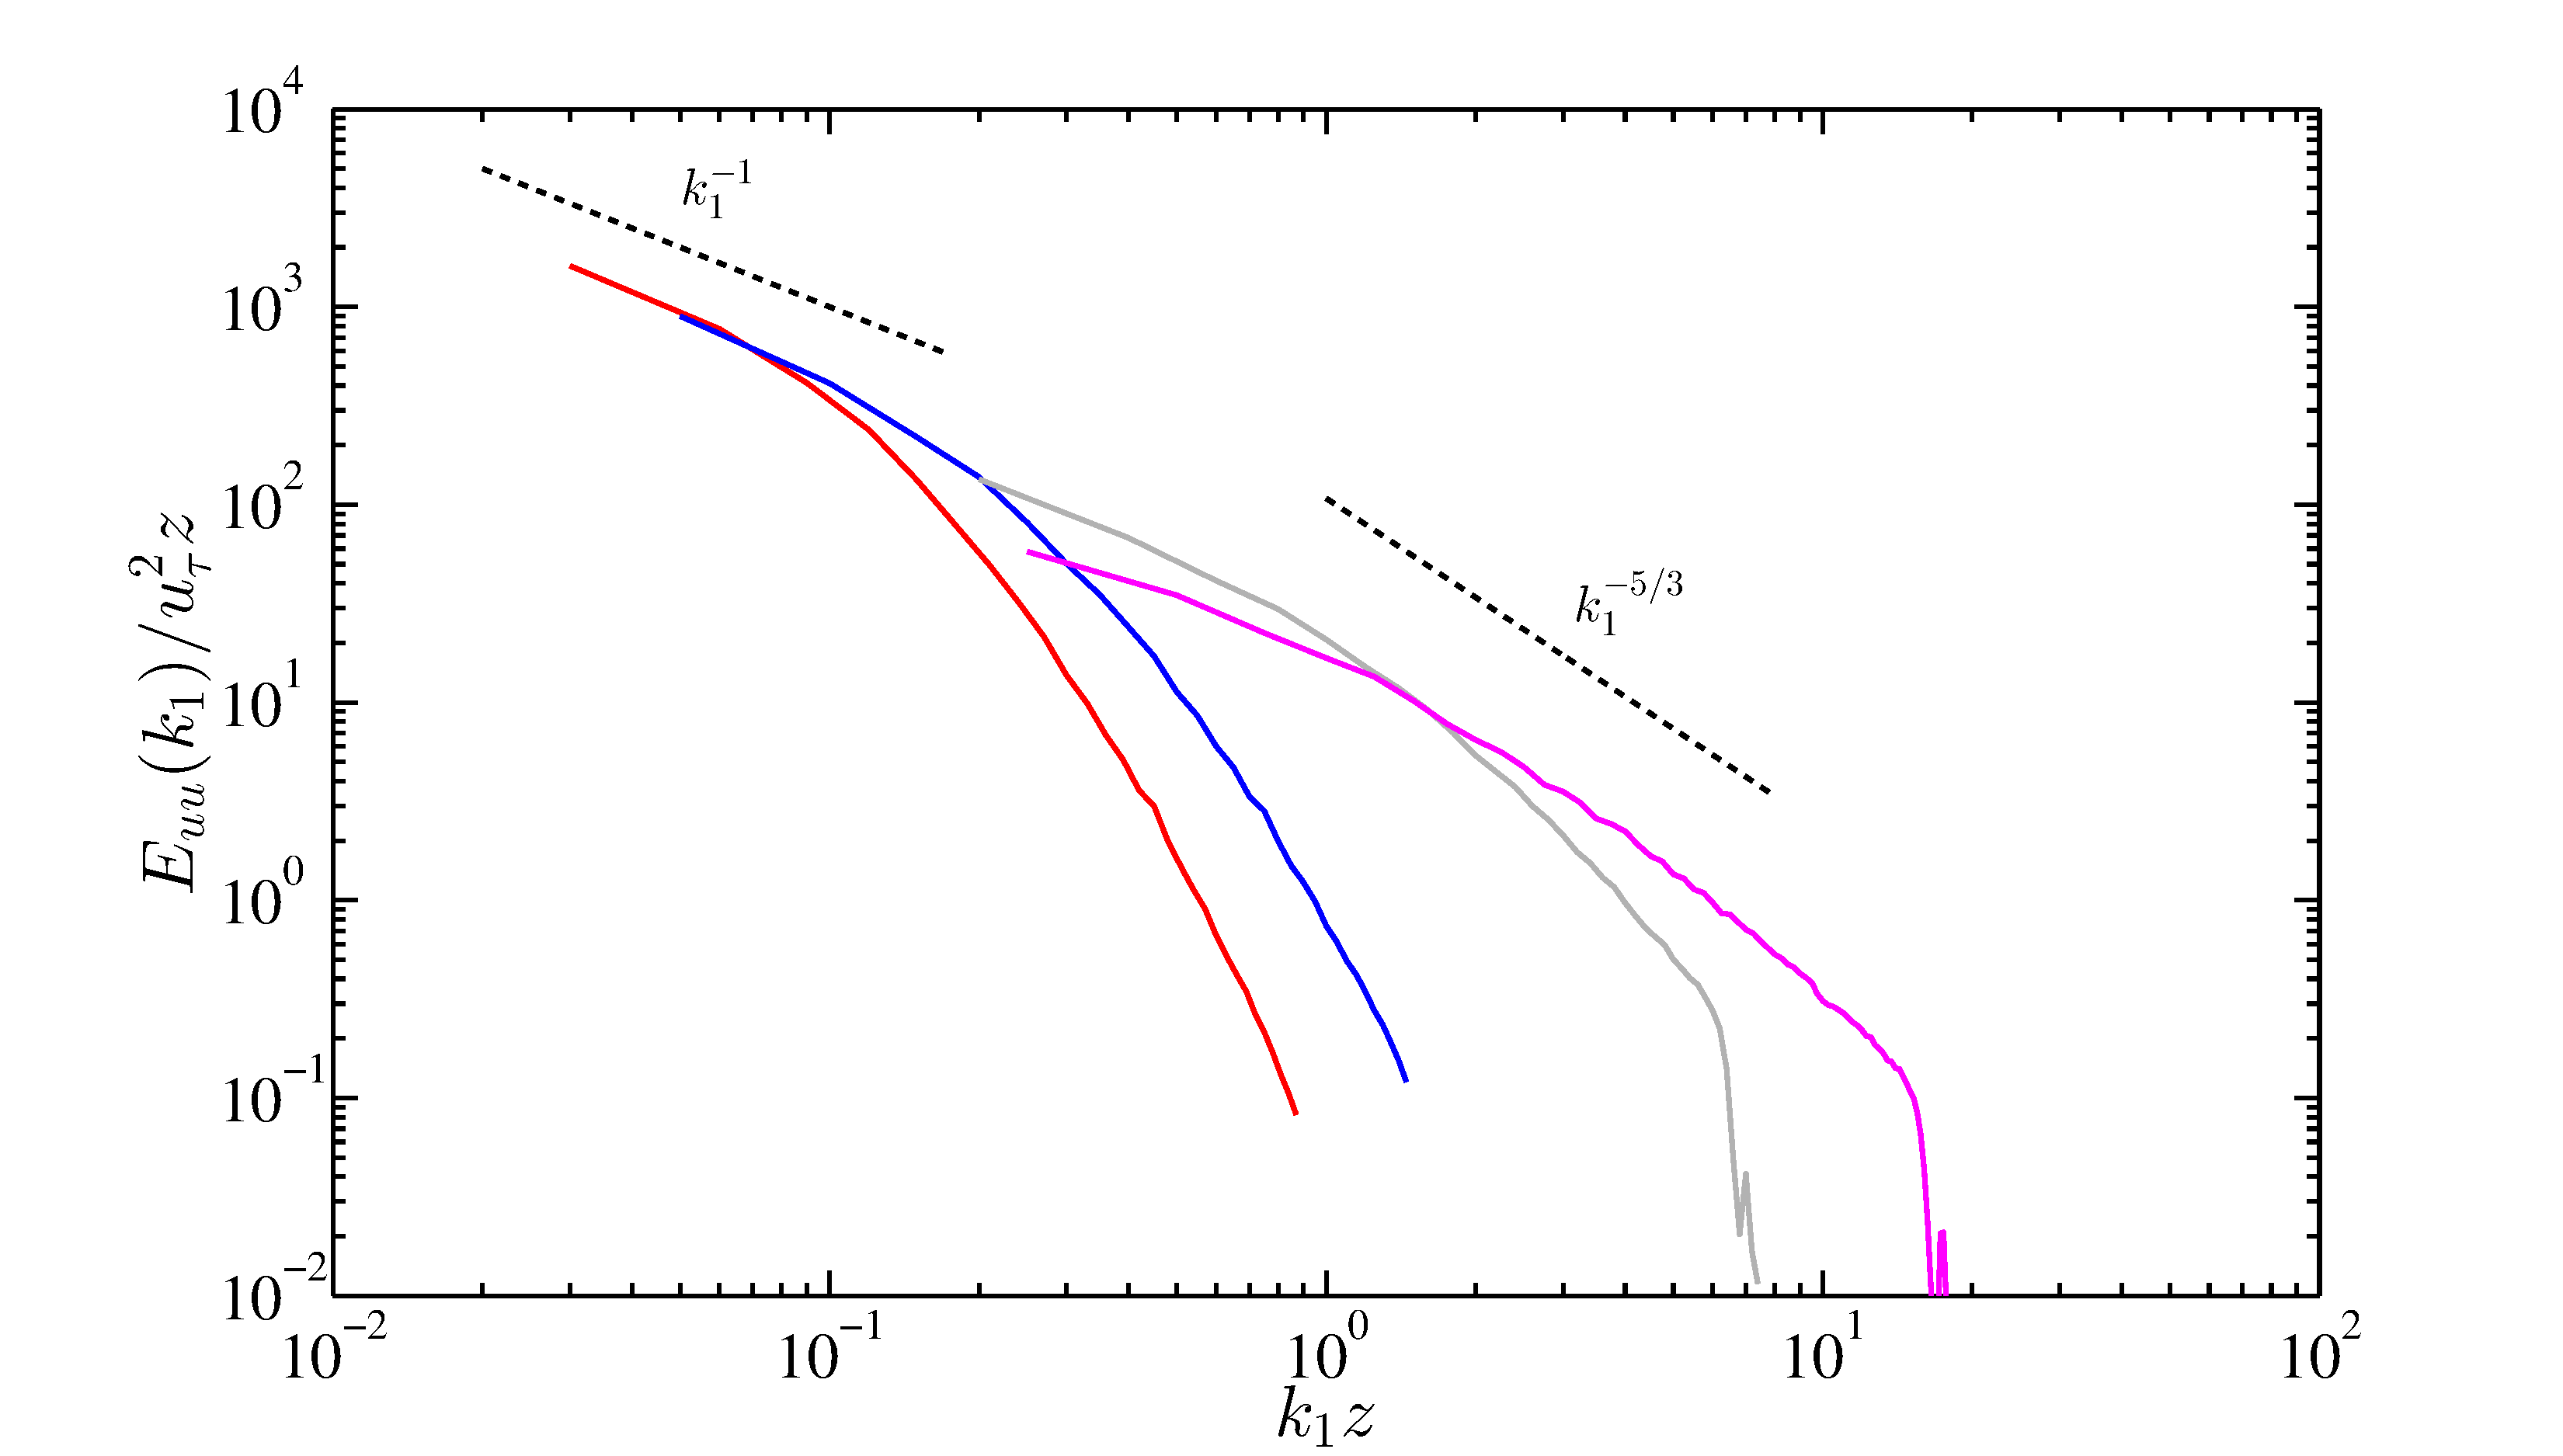
\includegraphics[width=\linewidth]{Fig2/energy_ABL_n2_filt4.pdf}
                \caption{}
                \label{fig:spec5}
        \end{subfigure}           
        \caption[1D Energy Spectra 2]{Temporally and Horizontally averaged streamwise energy spectrum (A) Case IX, $\lbrace C_0, \ n \rbrace = \lbrace 0.19 , 0.5 \rbrace$ (B) Case III, $\lbrace C_0, \ n \rbrace = \lbrace 0.16 , 2 \rbrace$, $k_c = 4$ is fixed. $k_1$ is the streamwise wavenumber. Red, $z/H = 0.015$, Blue, $z/H = 0.025$, Grey, $z/H = 0.1$, Magenta, $z/H = 0.25$  }\label{fig:stat0_lotw3}
\end{figure}

\begin{figure}
\centering
        \begin{subfigure}[t]{0.5\textwidth}
                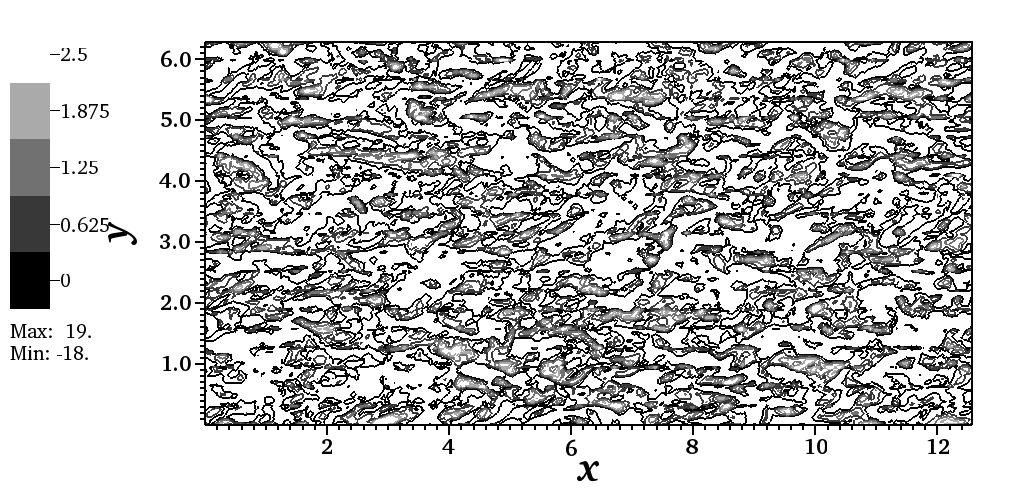
\includegraphics[width=\linewidth]{Fig2/x_vorticity_highdiff.png}
                \caption{}
                \label{fig:highdiff}
        \end{subfigure}%
        \centering
        \begin{subfigure}[t]{0.5\textwidth}
                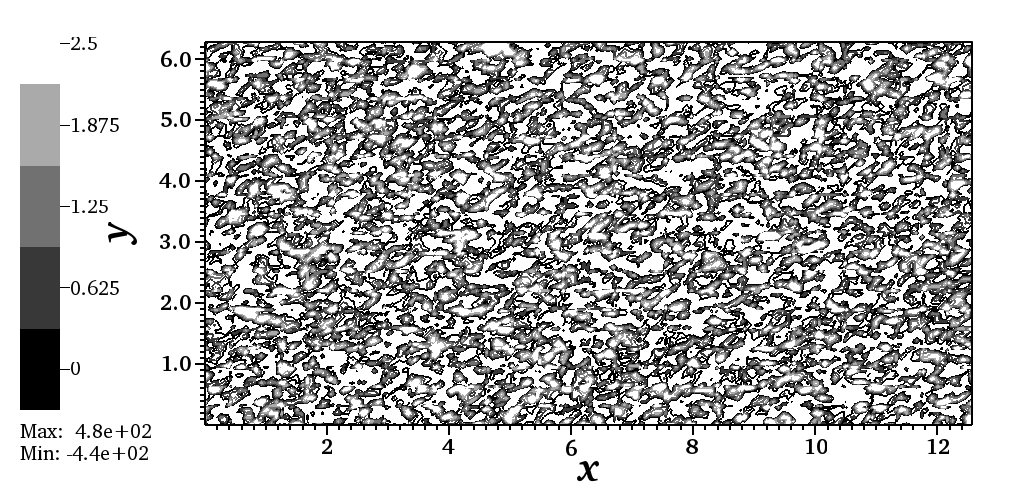
\includegraphics[width=\linewidth]{Fig2/x_vorticity_lowdiff.png}
                \caption{}
                \label{fig:lowdiff}
        \end{subfigure}
       \centering
        \begin{subfigure}[t]{0.5\textwidth}
                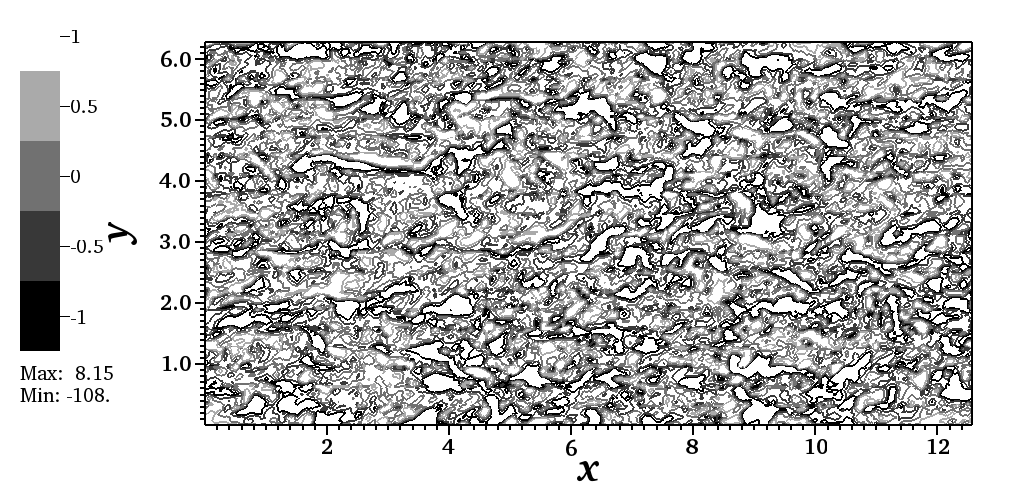
\includegraphics[width=\linewidth]{Fig2/z_vorticity_highdiff.png}
                \caption{}
                \label{fig:highdiff}
        \end{subfigure}%
        \centering
        \begin{subfigure}[t]{0.5\textwidth}
                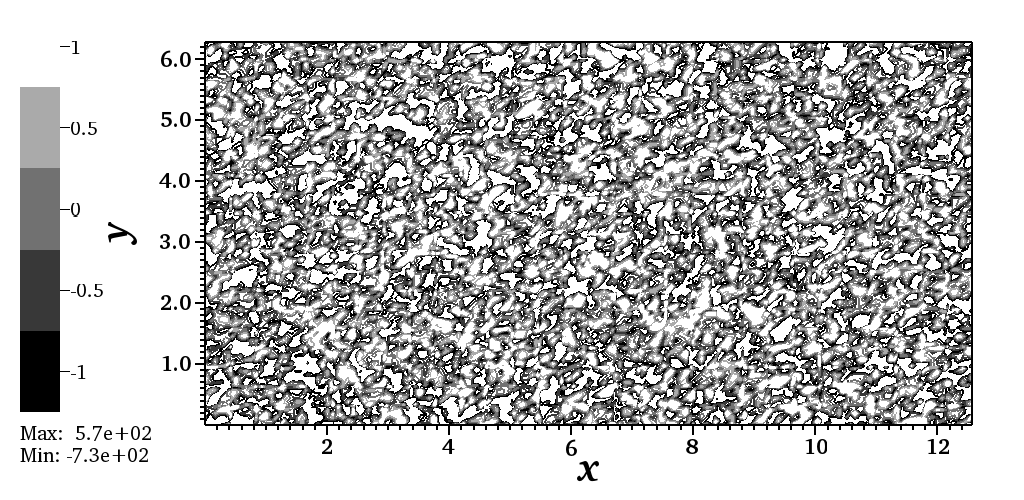
\includegraphics[width=\linewidth]{Fig2/z_vorticity_lowdiff.png}
                \caption{}
                \label{fig:lowdiff}
        \end{subfigure}%
        \caption[Near Wall vorticity structures]{ Instantaneous wall structures of $x$ (\textit{Top}), $z$ (\textit{Bottom}) vorticity  at log layer $z/H = 0.1$ (a) $\lbrace C_0 = 0.16,n = 2, k_c = 4\rbrace$ (b) $\lbrace C_0 = 0.19,n = 0.5, k_c = 4\rbrace $.}\label{fig:vort}
\end{figure}

\begin{figure}
\centering
        \begin{subfigure}[t]{0.5\textwidth}
                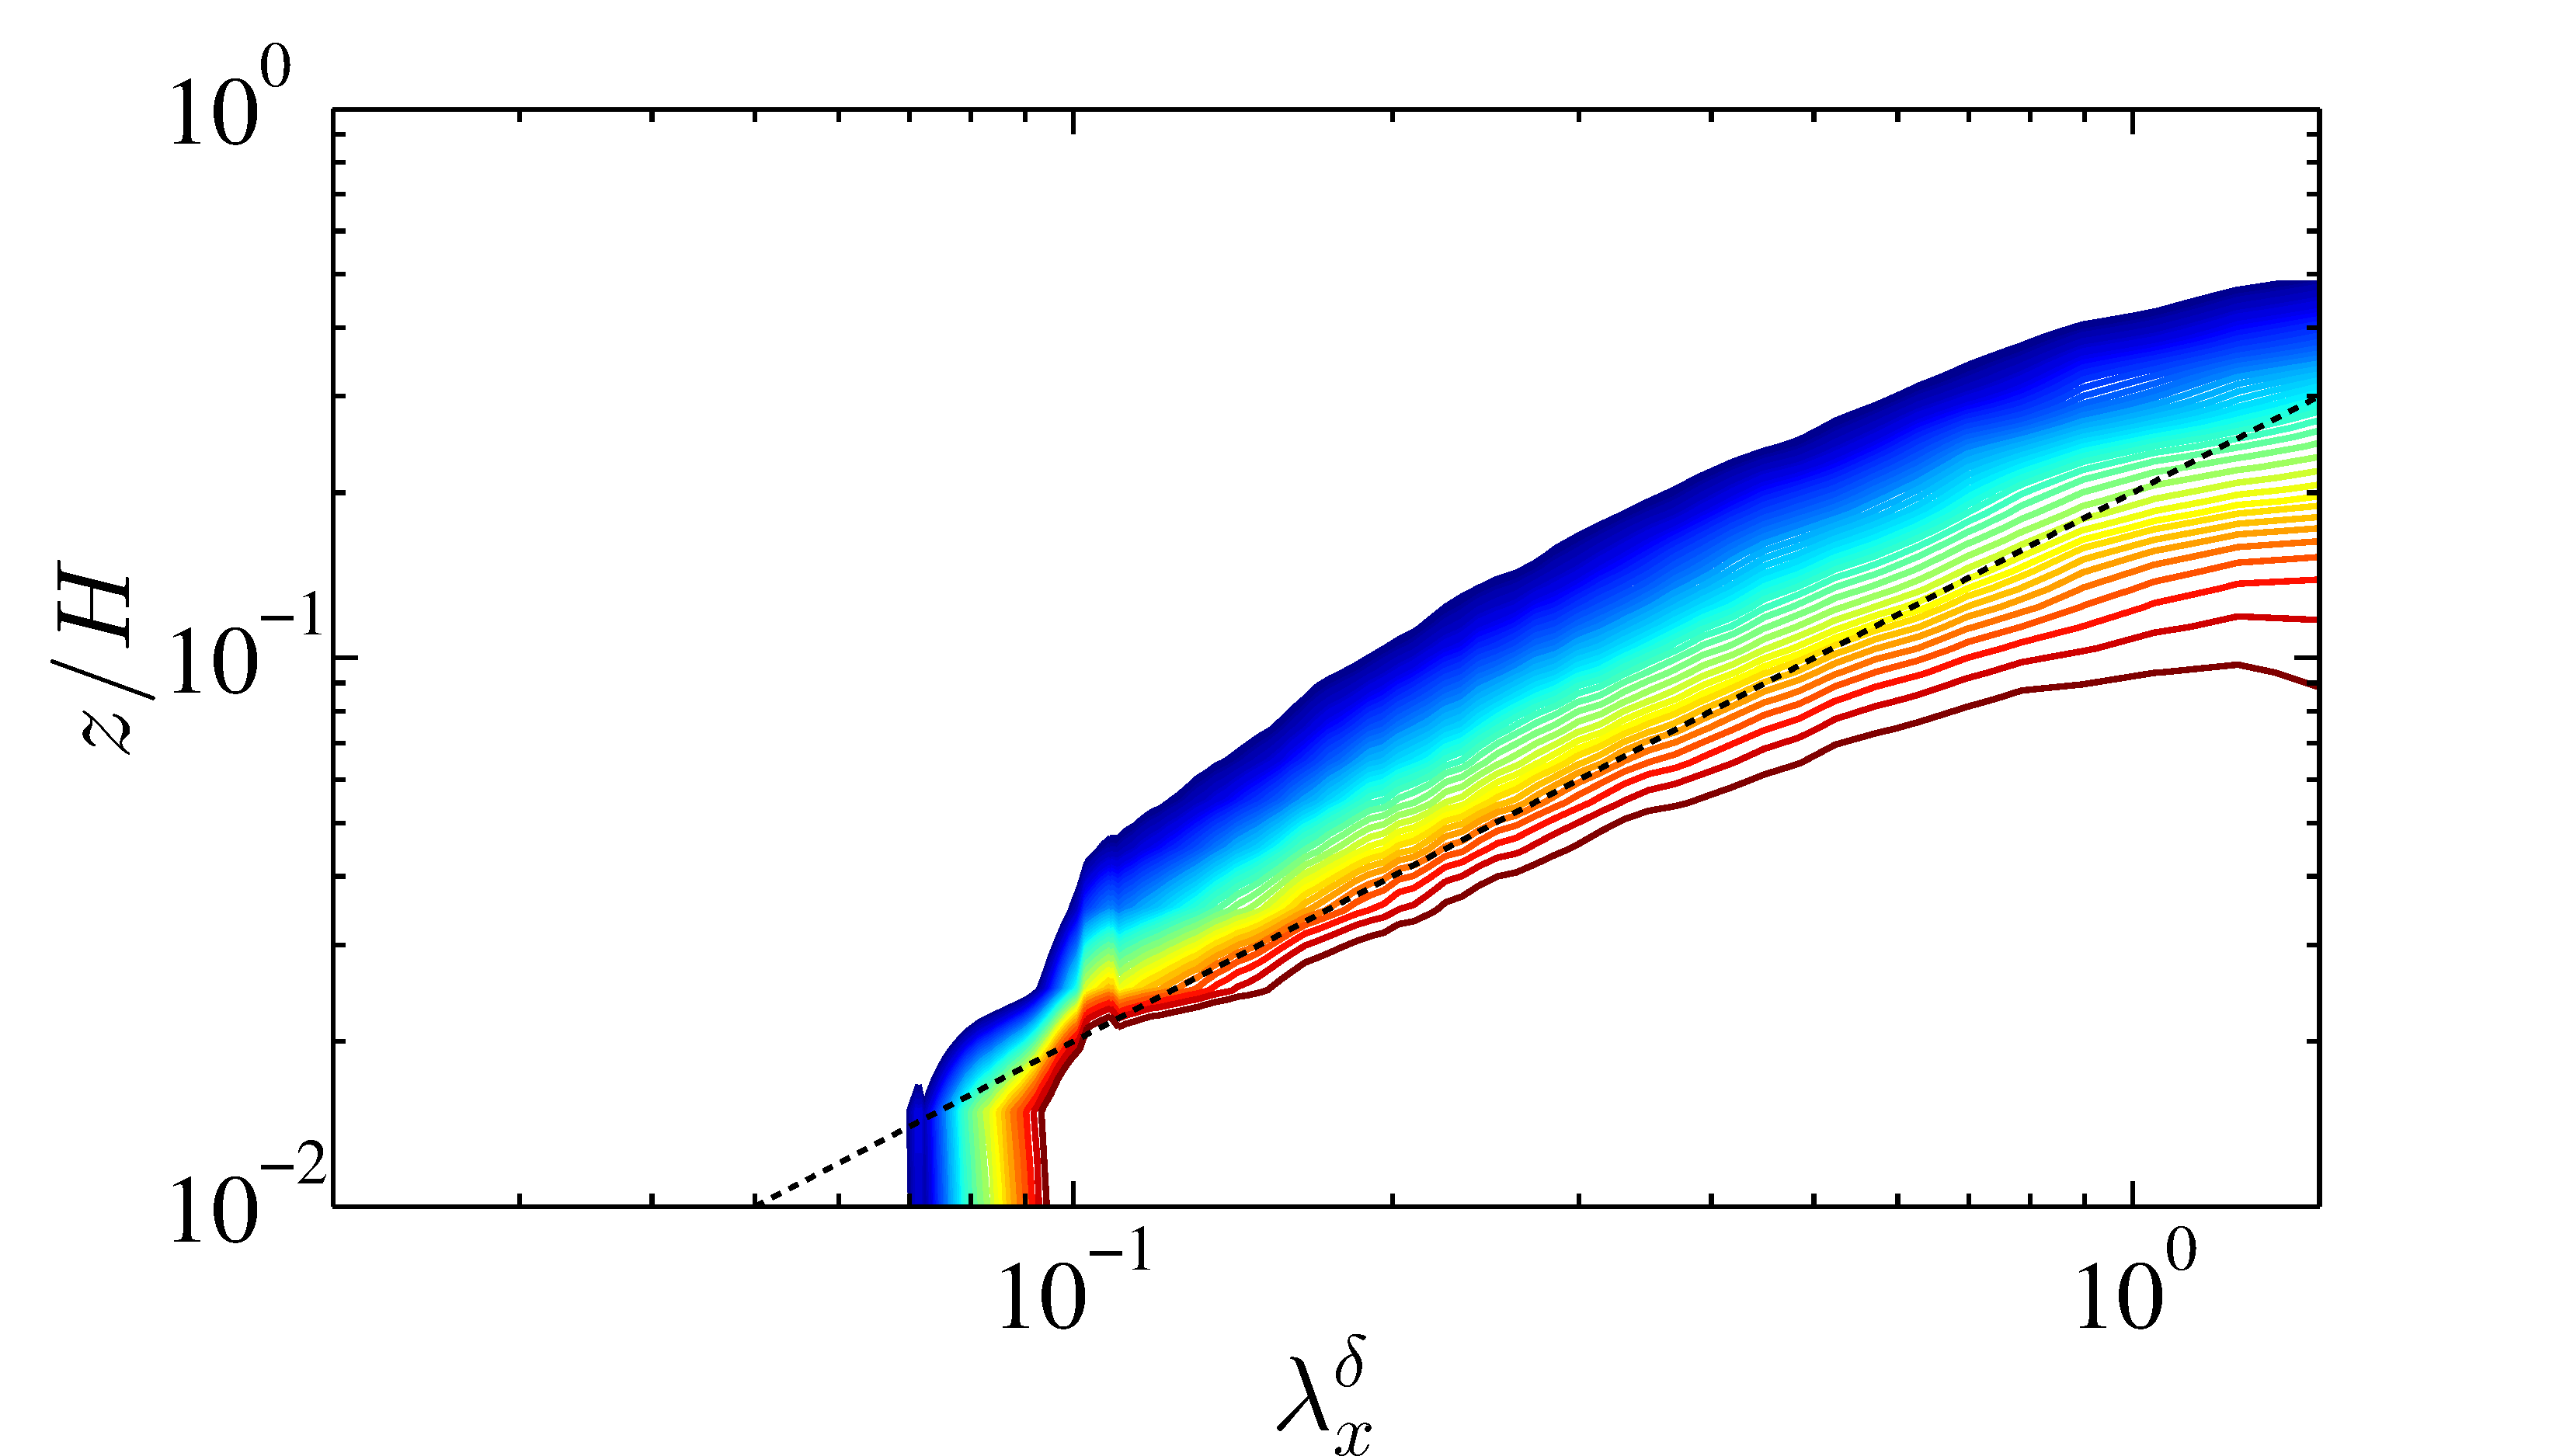
\includegraphics[width=\linewidth]{Fig2/energy_n05_logscale_85.pdf}
                \caption{}
                \label{fig:energy_n05}
        \end{subfigure}%
        \centering
        \begin{subfigure}[t]{0.5\textwidth}
                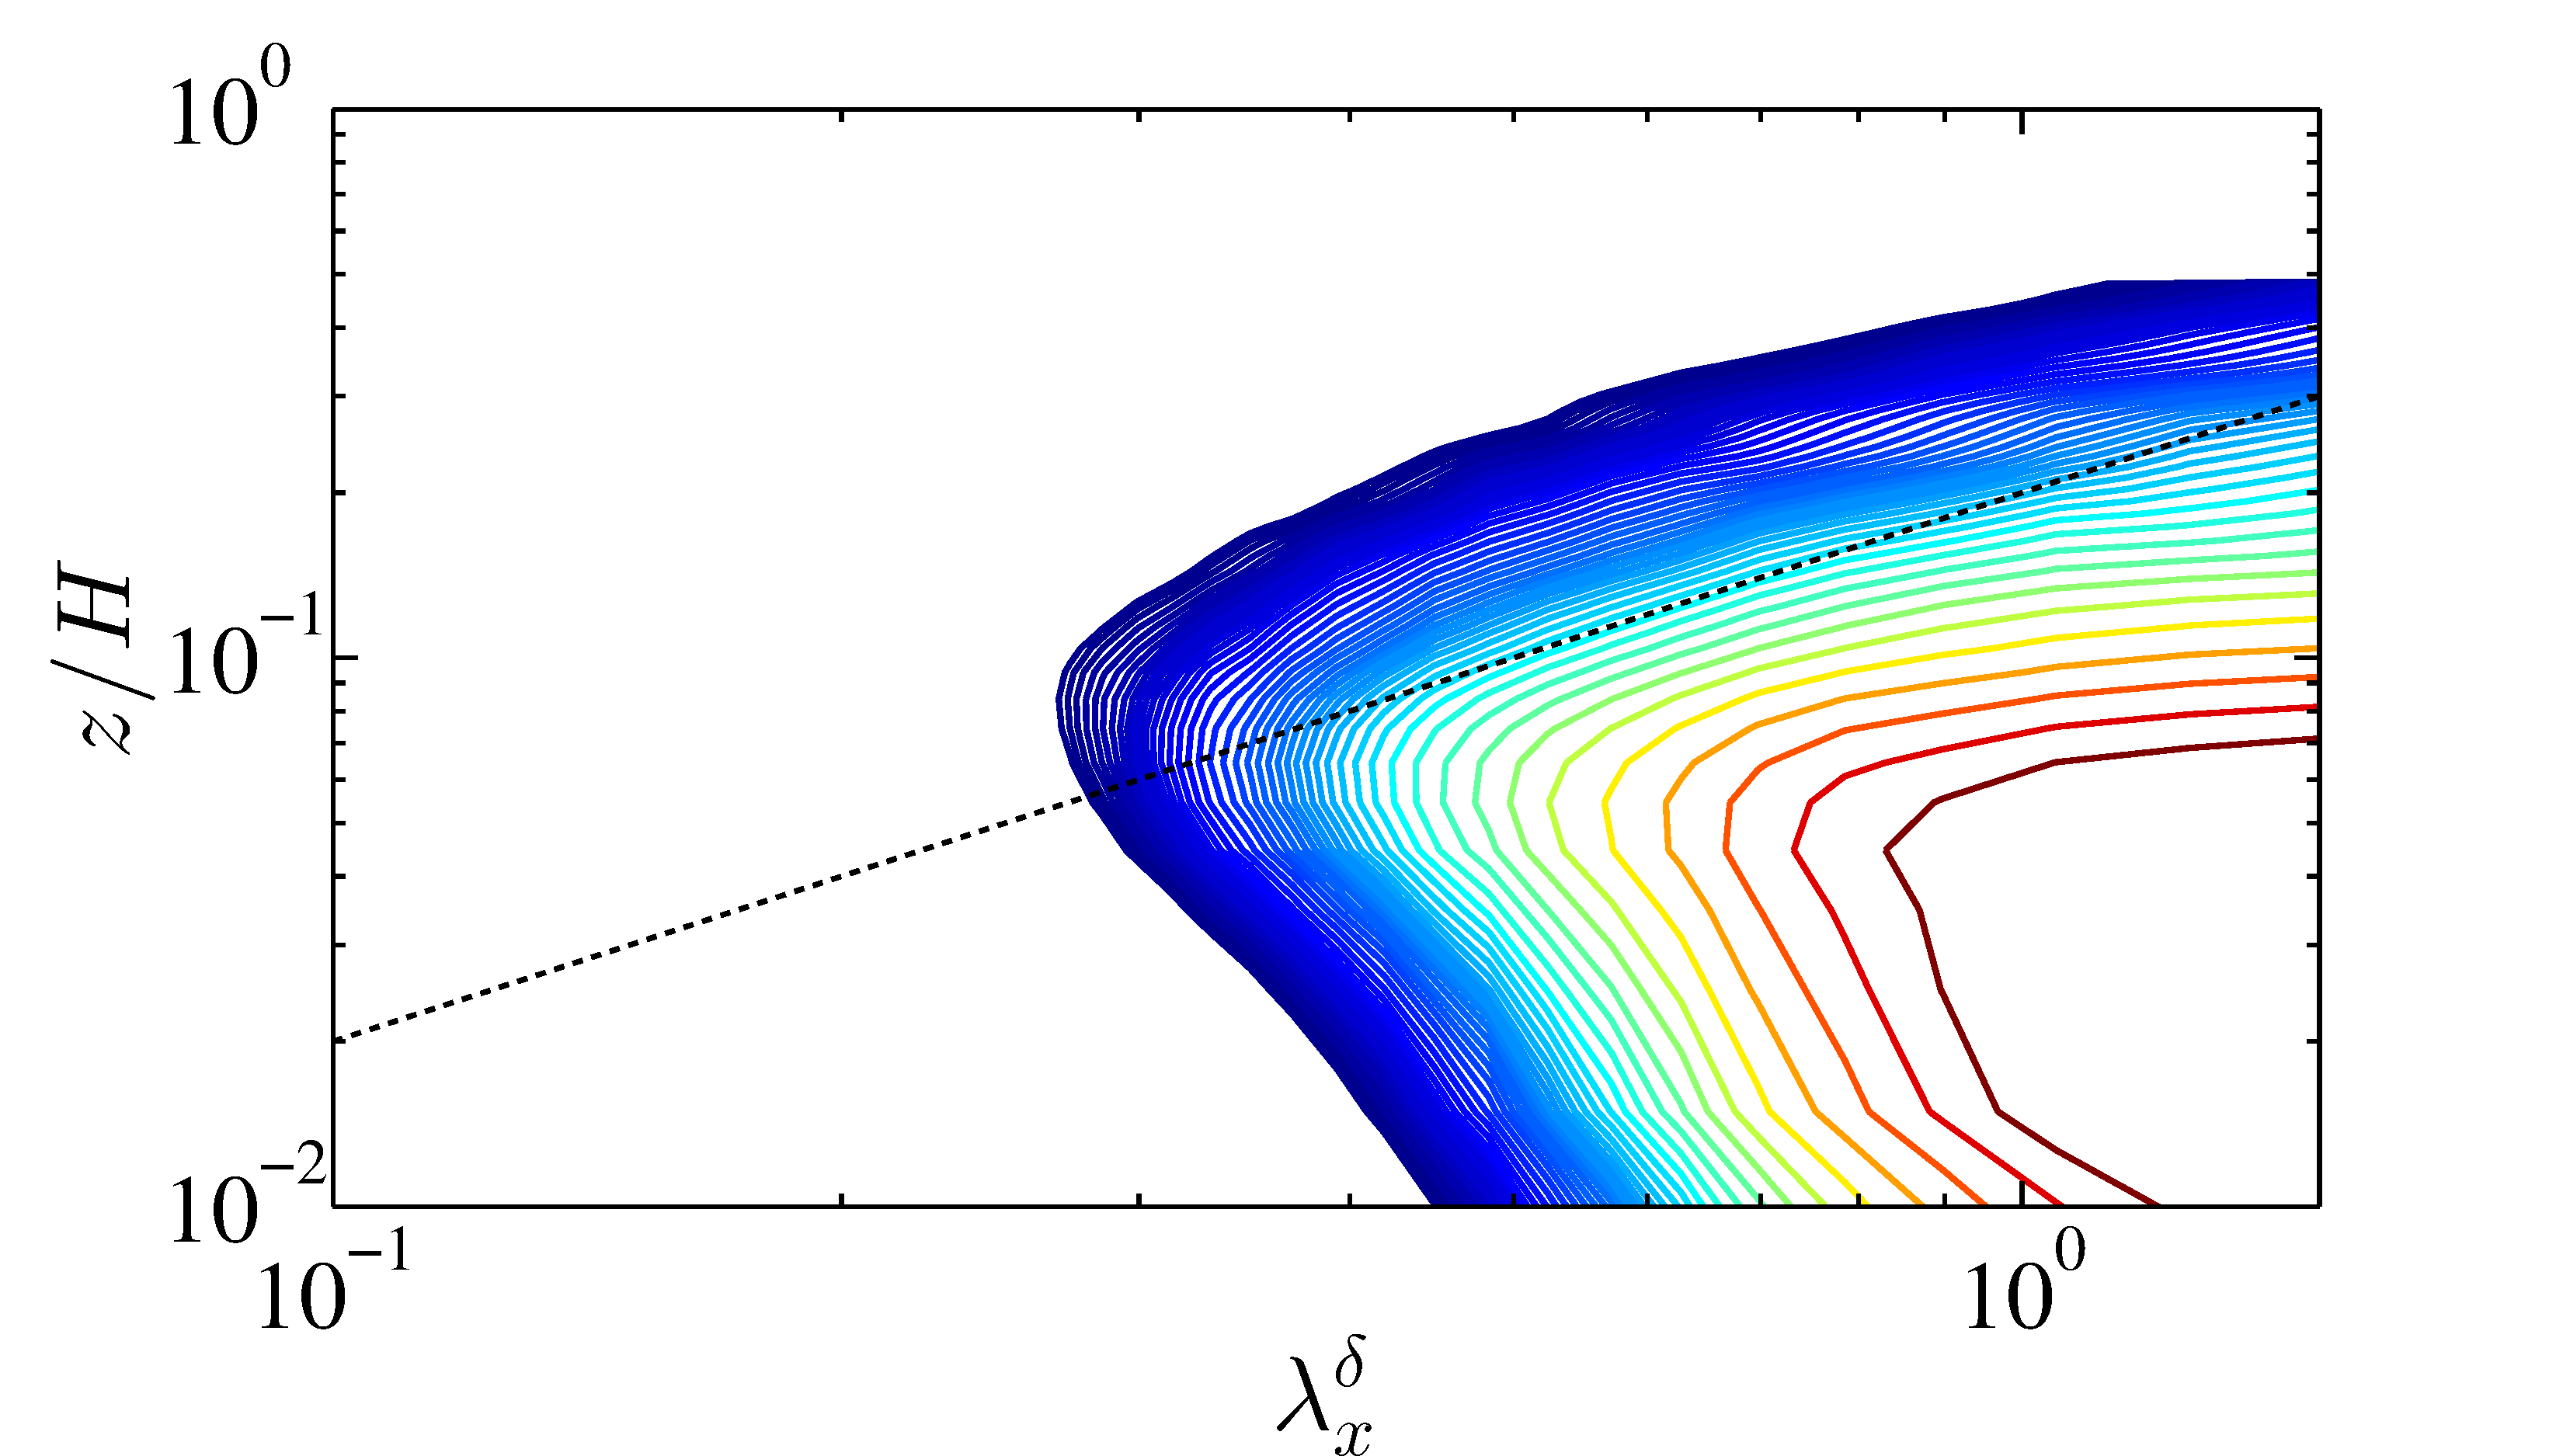
\includegraphics[width=\linewidth]{Fig2/energy_n2_logscale_85.pdf}
                \label{fig:energy_n2}
        \end{subfigure}%
        \caption[Log variation of Energy]{Variation of horizontally and temporally averaged Premultiplied energy spectra $k_1E_{uu}(k_1)$ over wall-normal distance $z/H$ and normalized length scale $\lambda^{\delta}_{x}$ (A) Case IX, $\lbrace C_0 = 0.19,n = 0.5, k_c = 4\rbrace $ (B) Case III, $\lbrace C_0 = 0.16,n = 2, k_c = 4\rbrace $. $\lambda^{\delta}_{x} = \frac{\lambda_x}{H}$, is the normalized streamwise wavelength. $\lambda_x = \frac{2\pi}{k_1}$. Dashed line represents $\lambda_x^{\delta} = 5z/H$. Contour levels indicate $0.85$ times the maximum value at each $z$ level.}\label{fig:2d_spec}
\end{figure}

\begin{figure}
\centering
        \begin{subfigure}[t]{0.5\textwidth}
                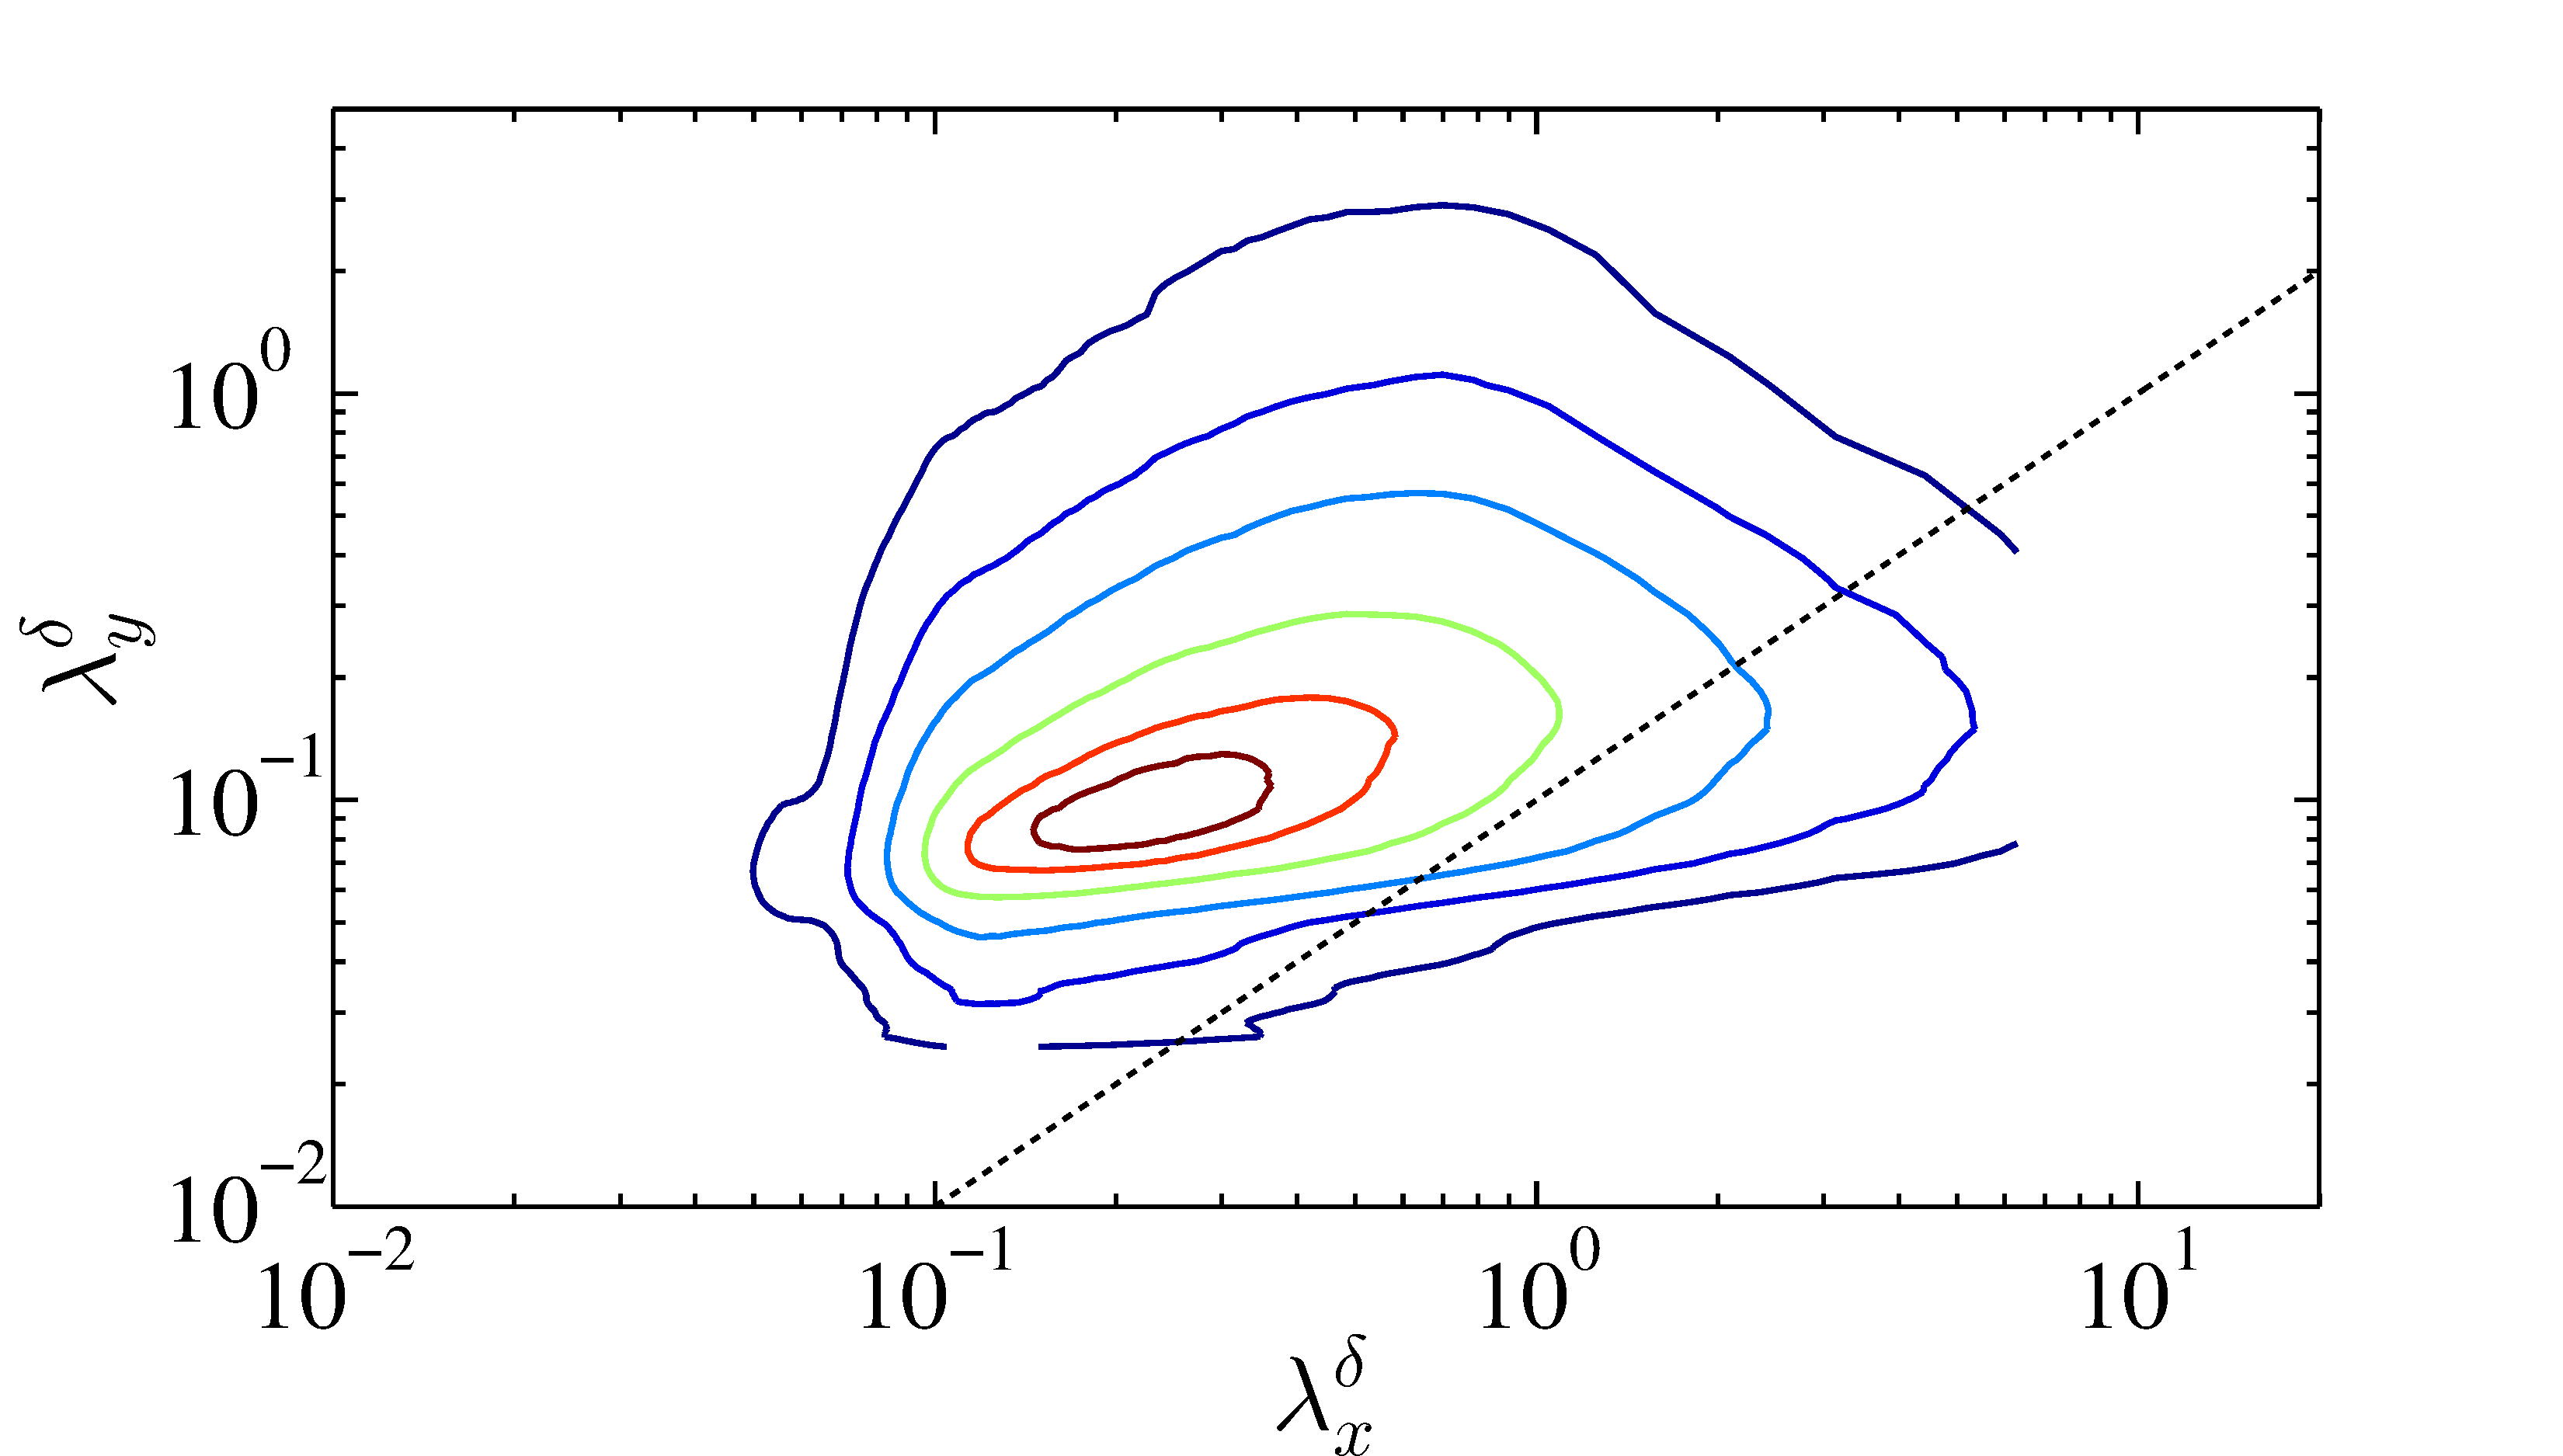
\includegraphics[width=\linewidth]{Fig2/energy_contour_ABL_n05_filt2_level2.pdf}
                \caption{}
                \label{fig:energy1}
        \end{subfigure}%
        \centering
        \begin{subfigure}[t]{0.5\textwidth}
                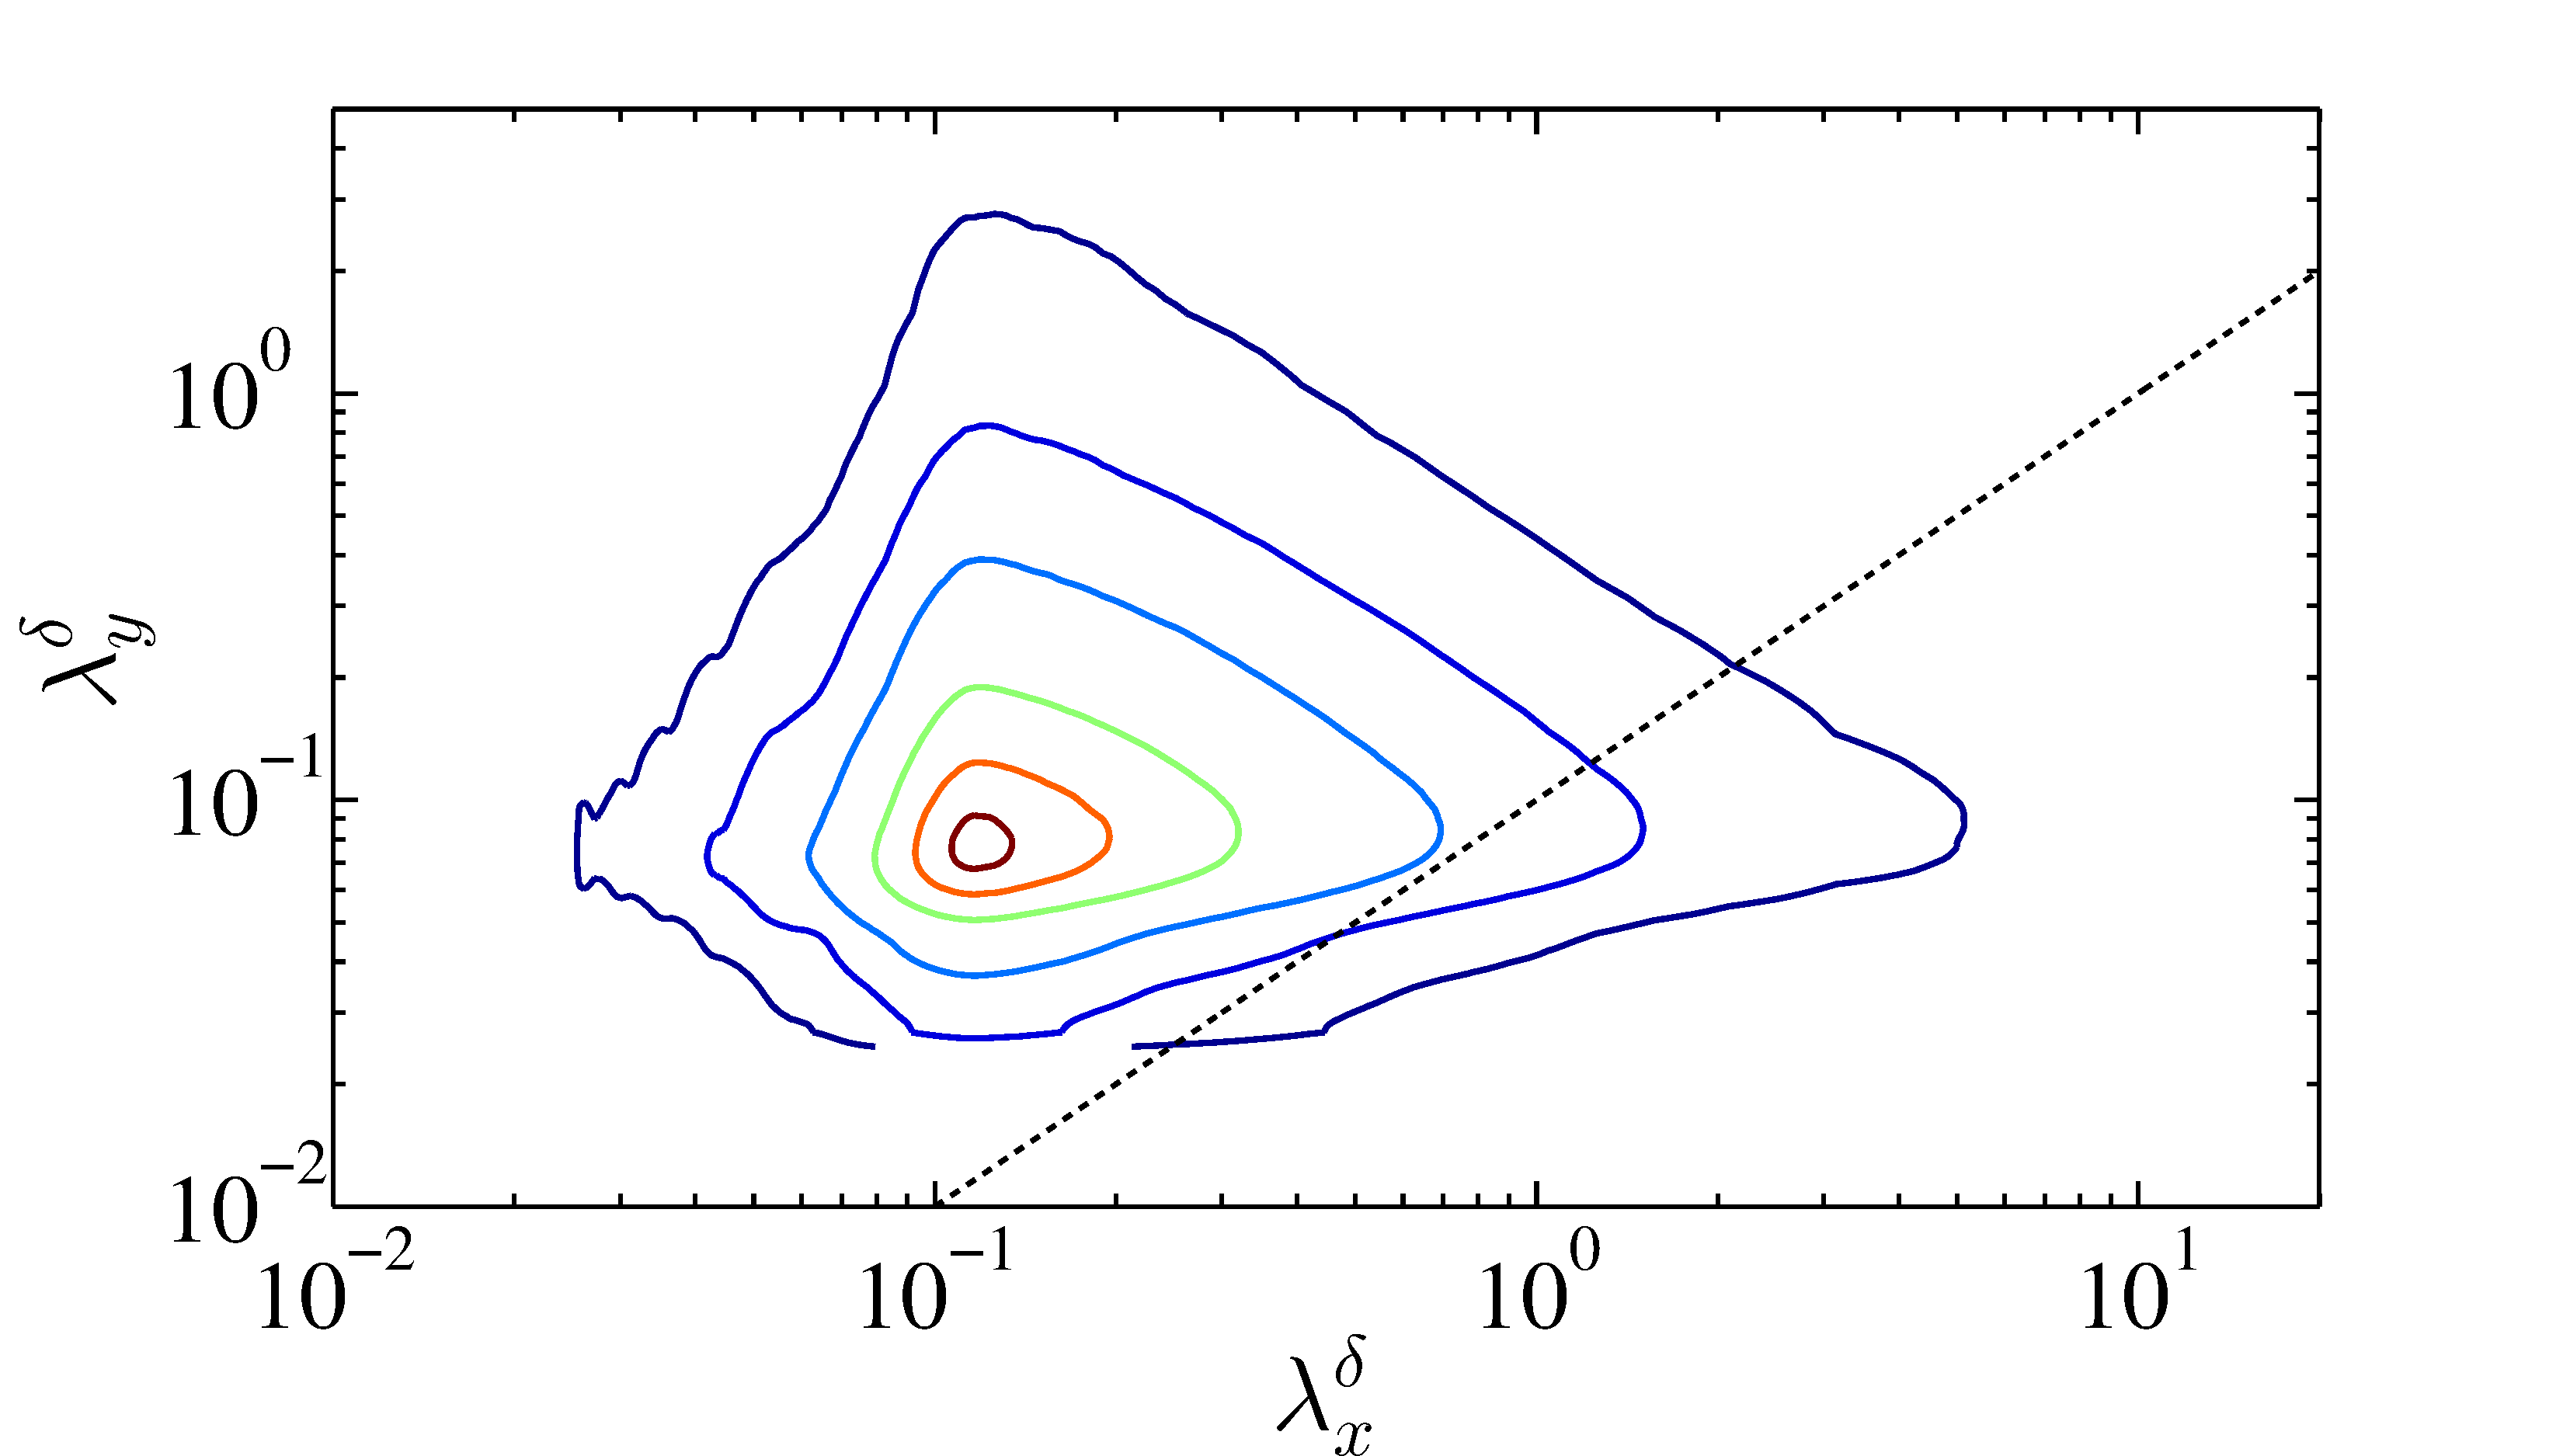
\includegraphics[width=\linewidth]{Fig2/dissp_contour_ABL_n05_filt2_level2.pdf}
                \caption{}
                \label{fig:dissip1}
        \end{subfigure}
\centering
        \begin{subfigure}[t]{0.5\textwidth}
                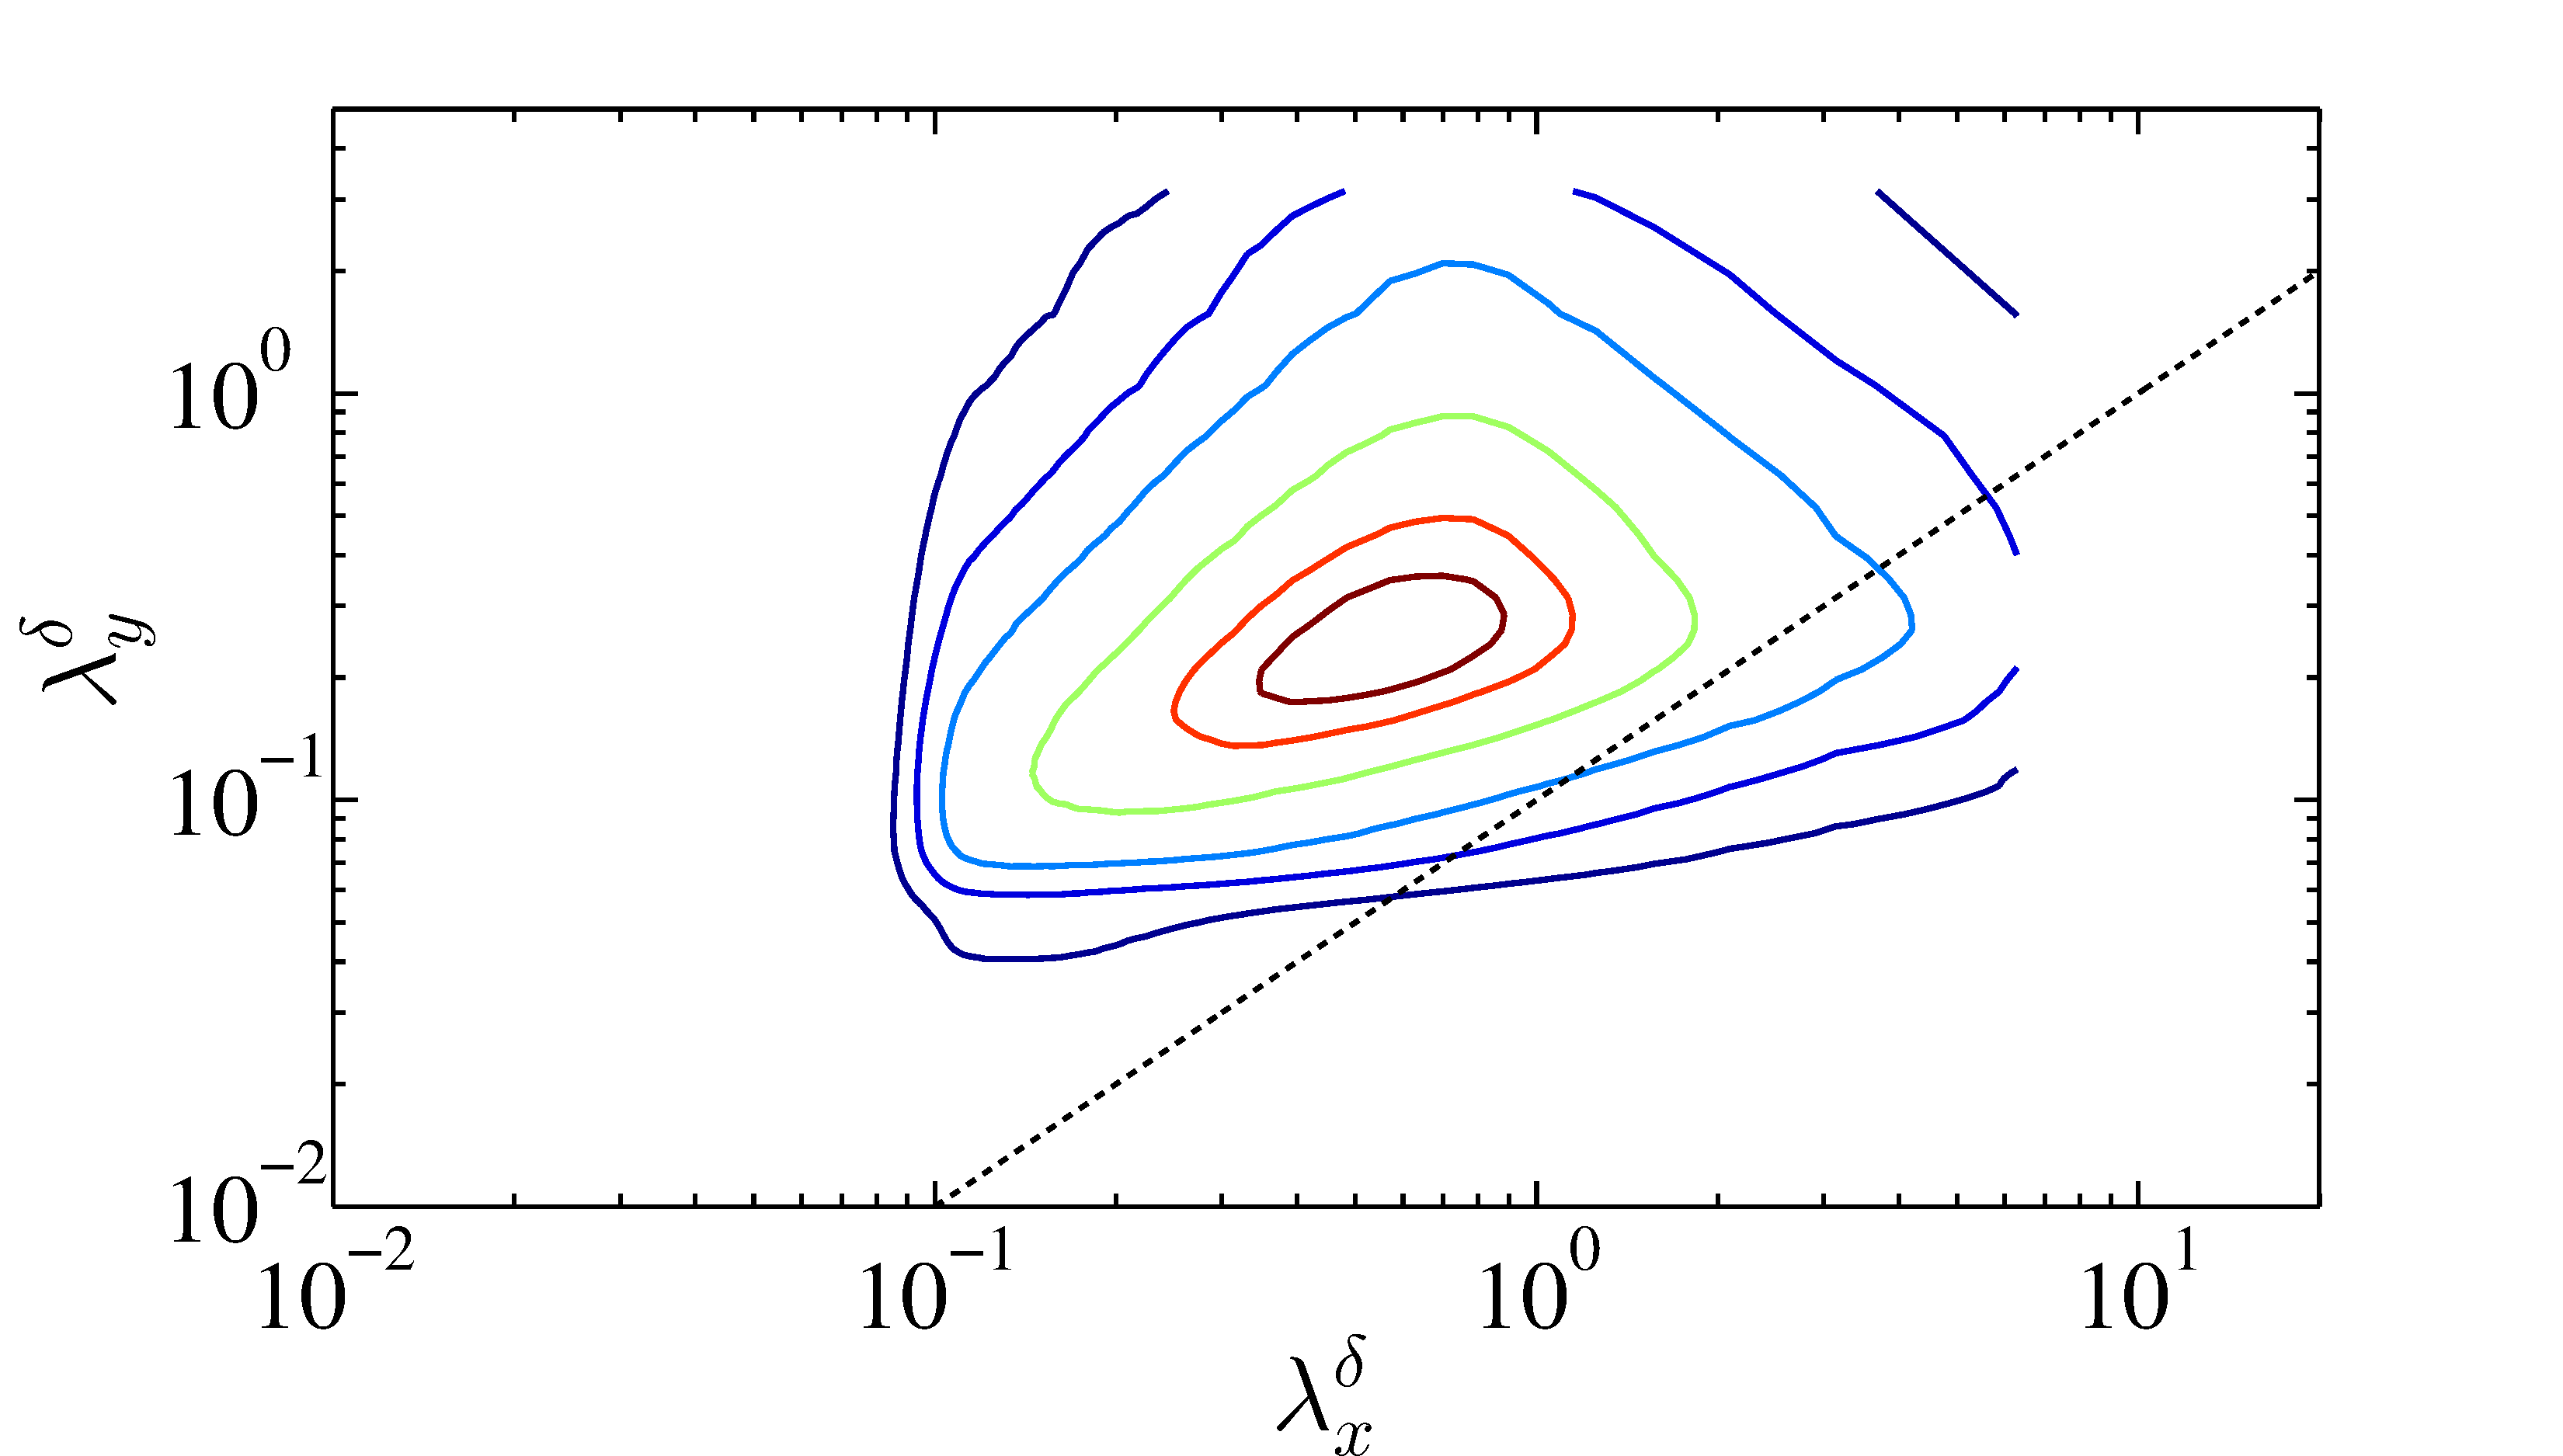
\includegraphics[width=\linewidth]{Fig2/energy_contour_ABL_n05_filt2_level4.pdf}
                \caption{}
                \label{fig:energy2}
        \end{subfigure}%
        \centering
        \begin{subfigure}[t]{0.5\textwidth}
                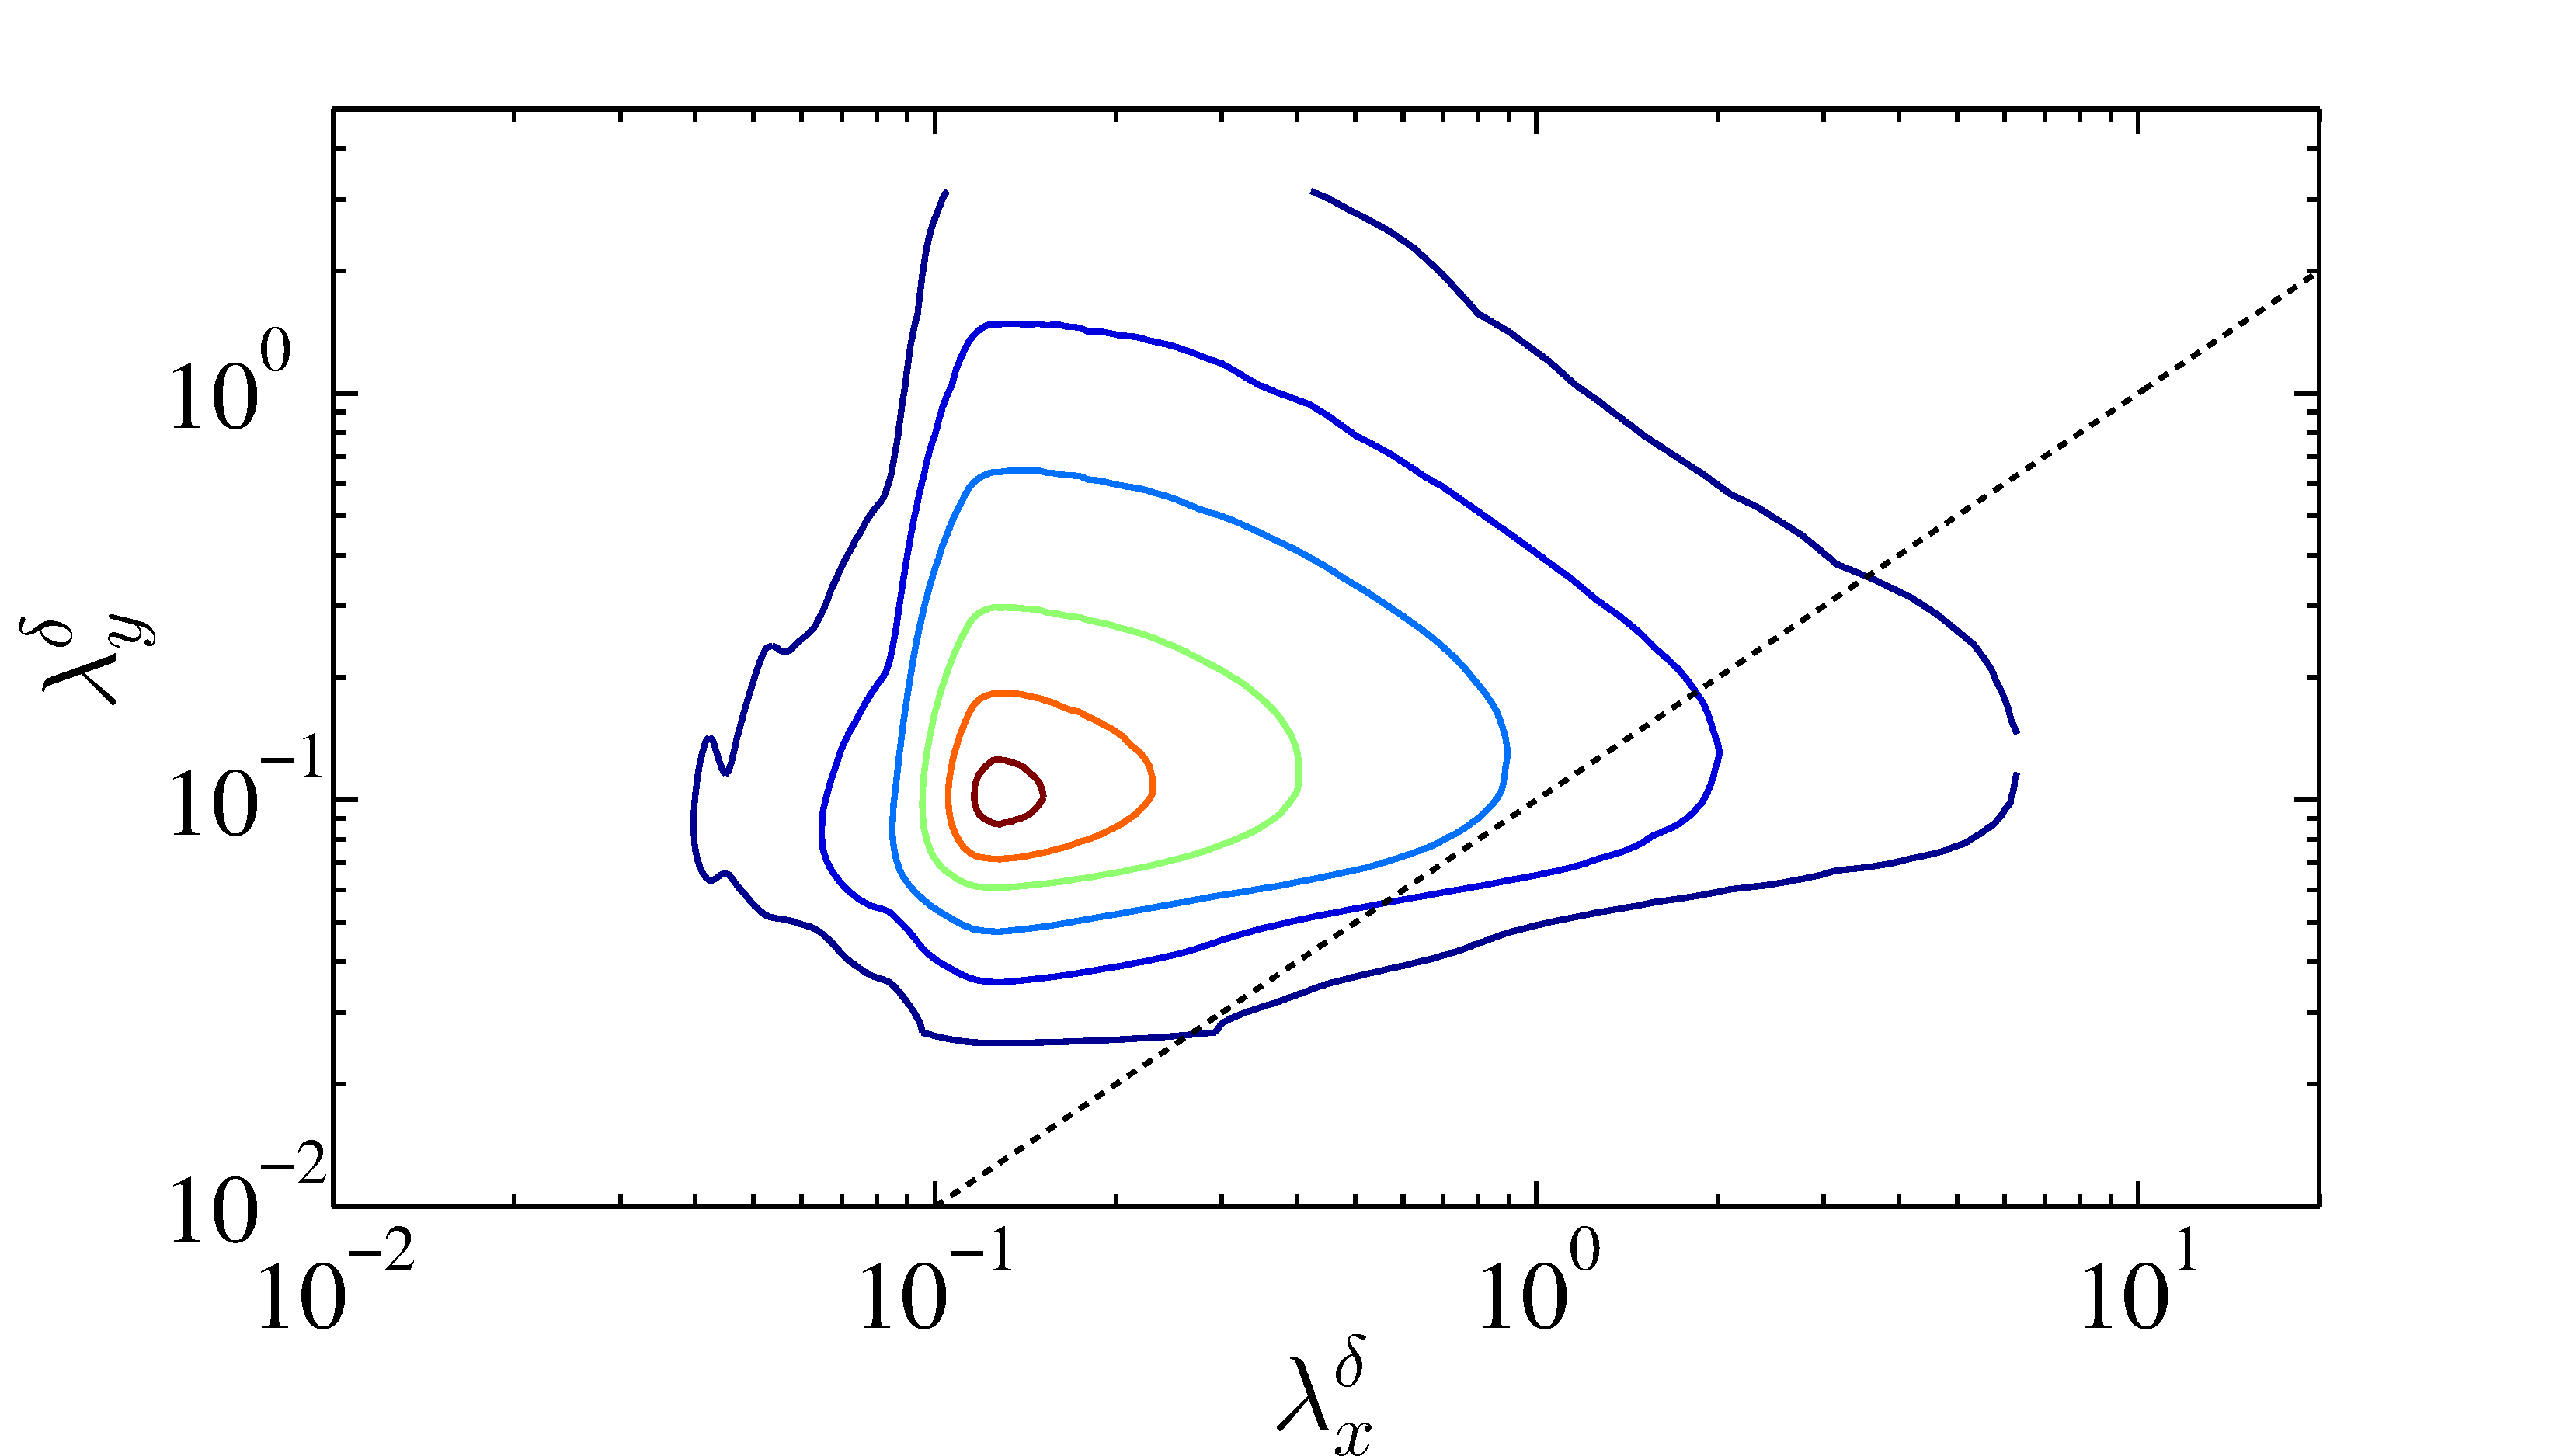
\includegraphics[width=\linewidth]{Fig2/dissp_contour_ABL_n05_filt2_level4.pdf}
                \caption{}
                \label{fig:dissip2}
        \end{subfigure}
 \centering
        \begin{subfigure}[t]{0.5\textwidth}
                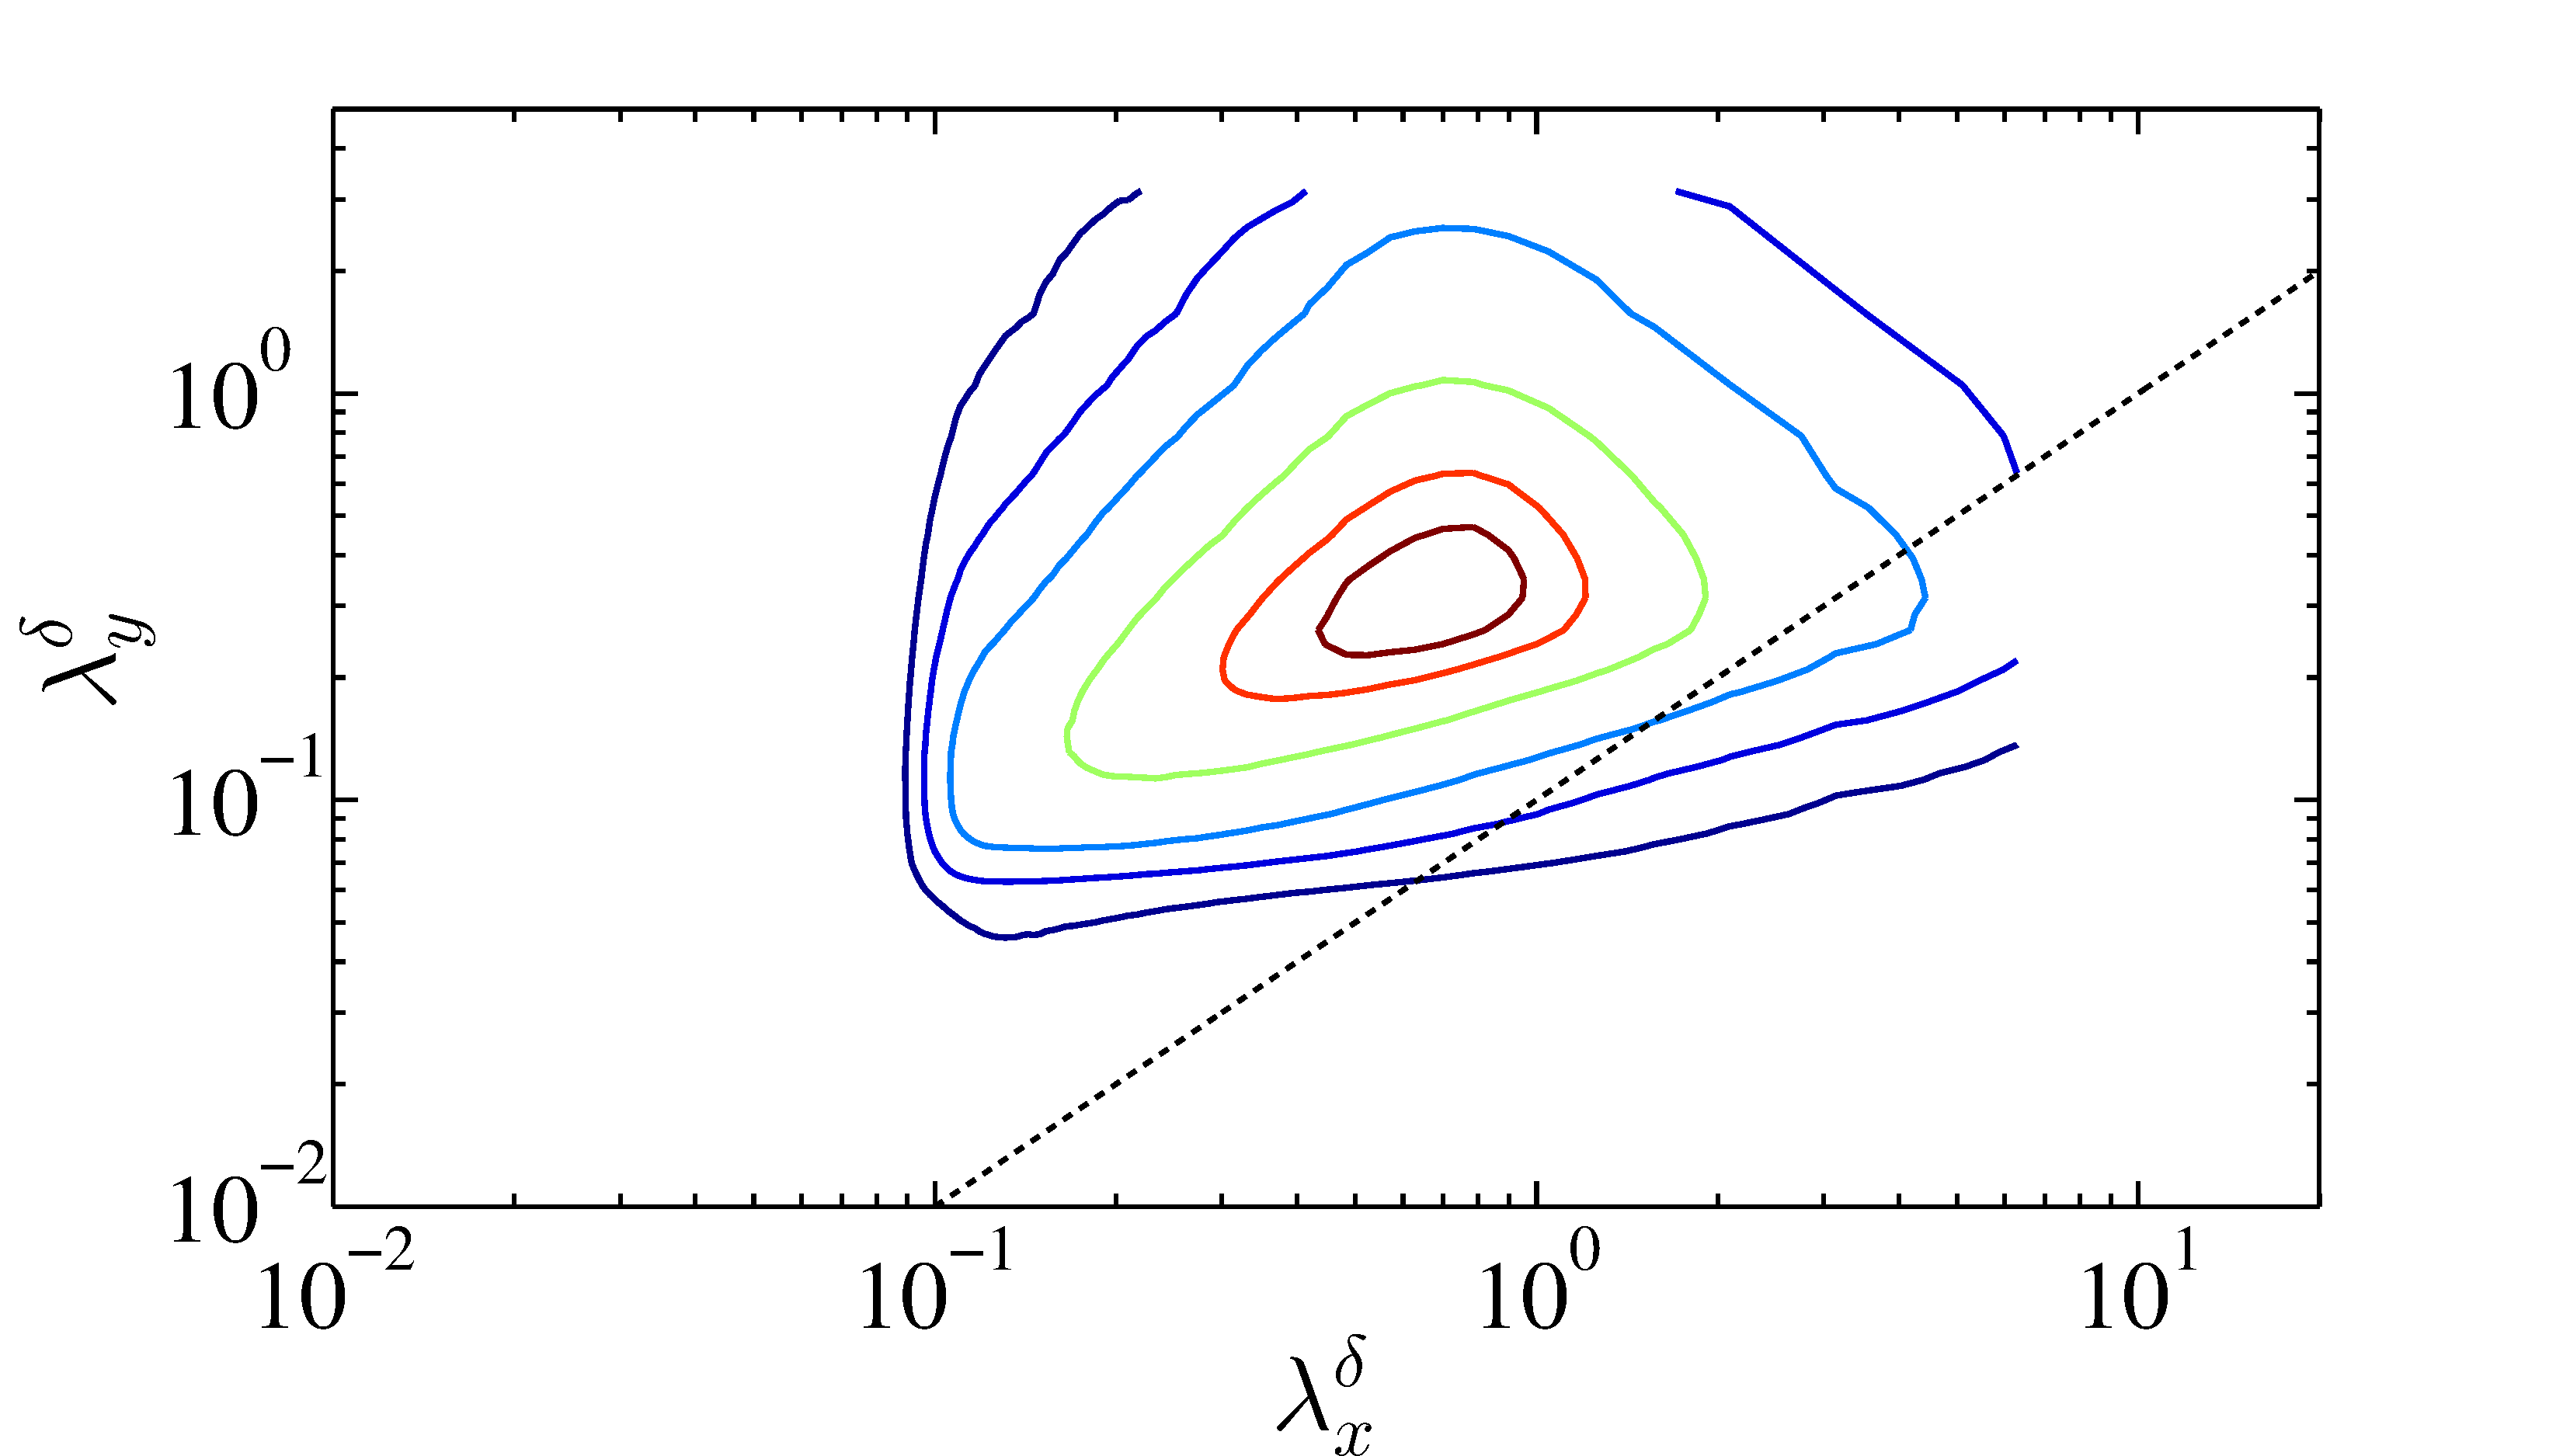
\includegraphics[width=\linewidth]{Fig2/energy_contour_ABL_n05_filt2_level5.pdf}
                \caption{}
                \label{fig:energy3}
        \end{subfigure}%
        \centering
        \begin{subfigure}[t]{0.5\textwidth}
                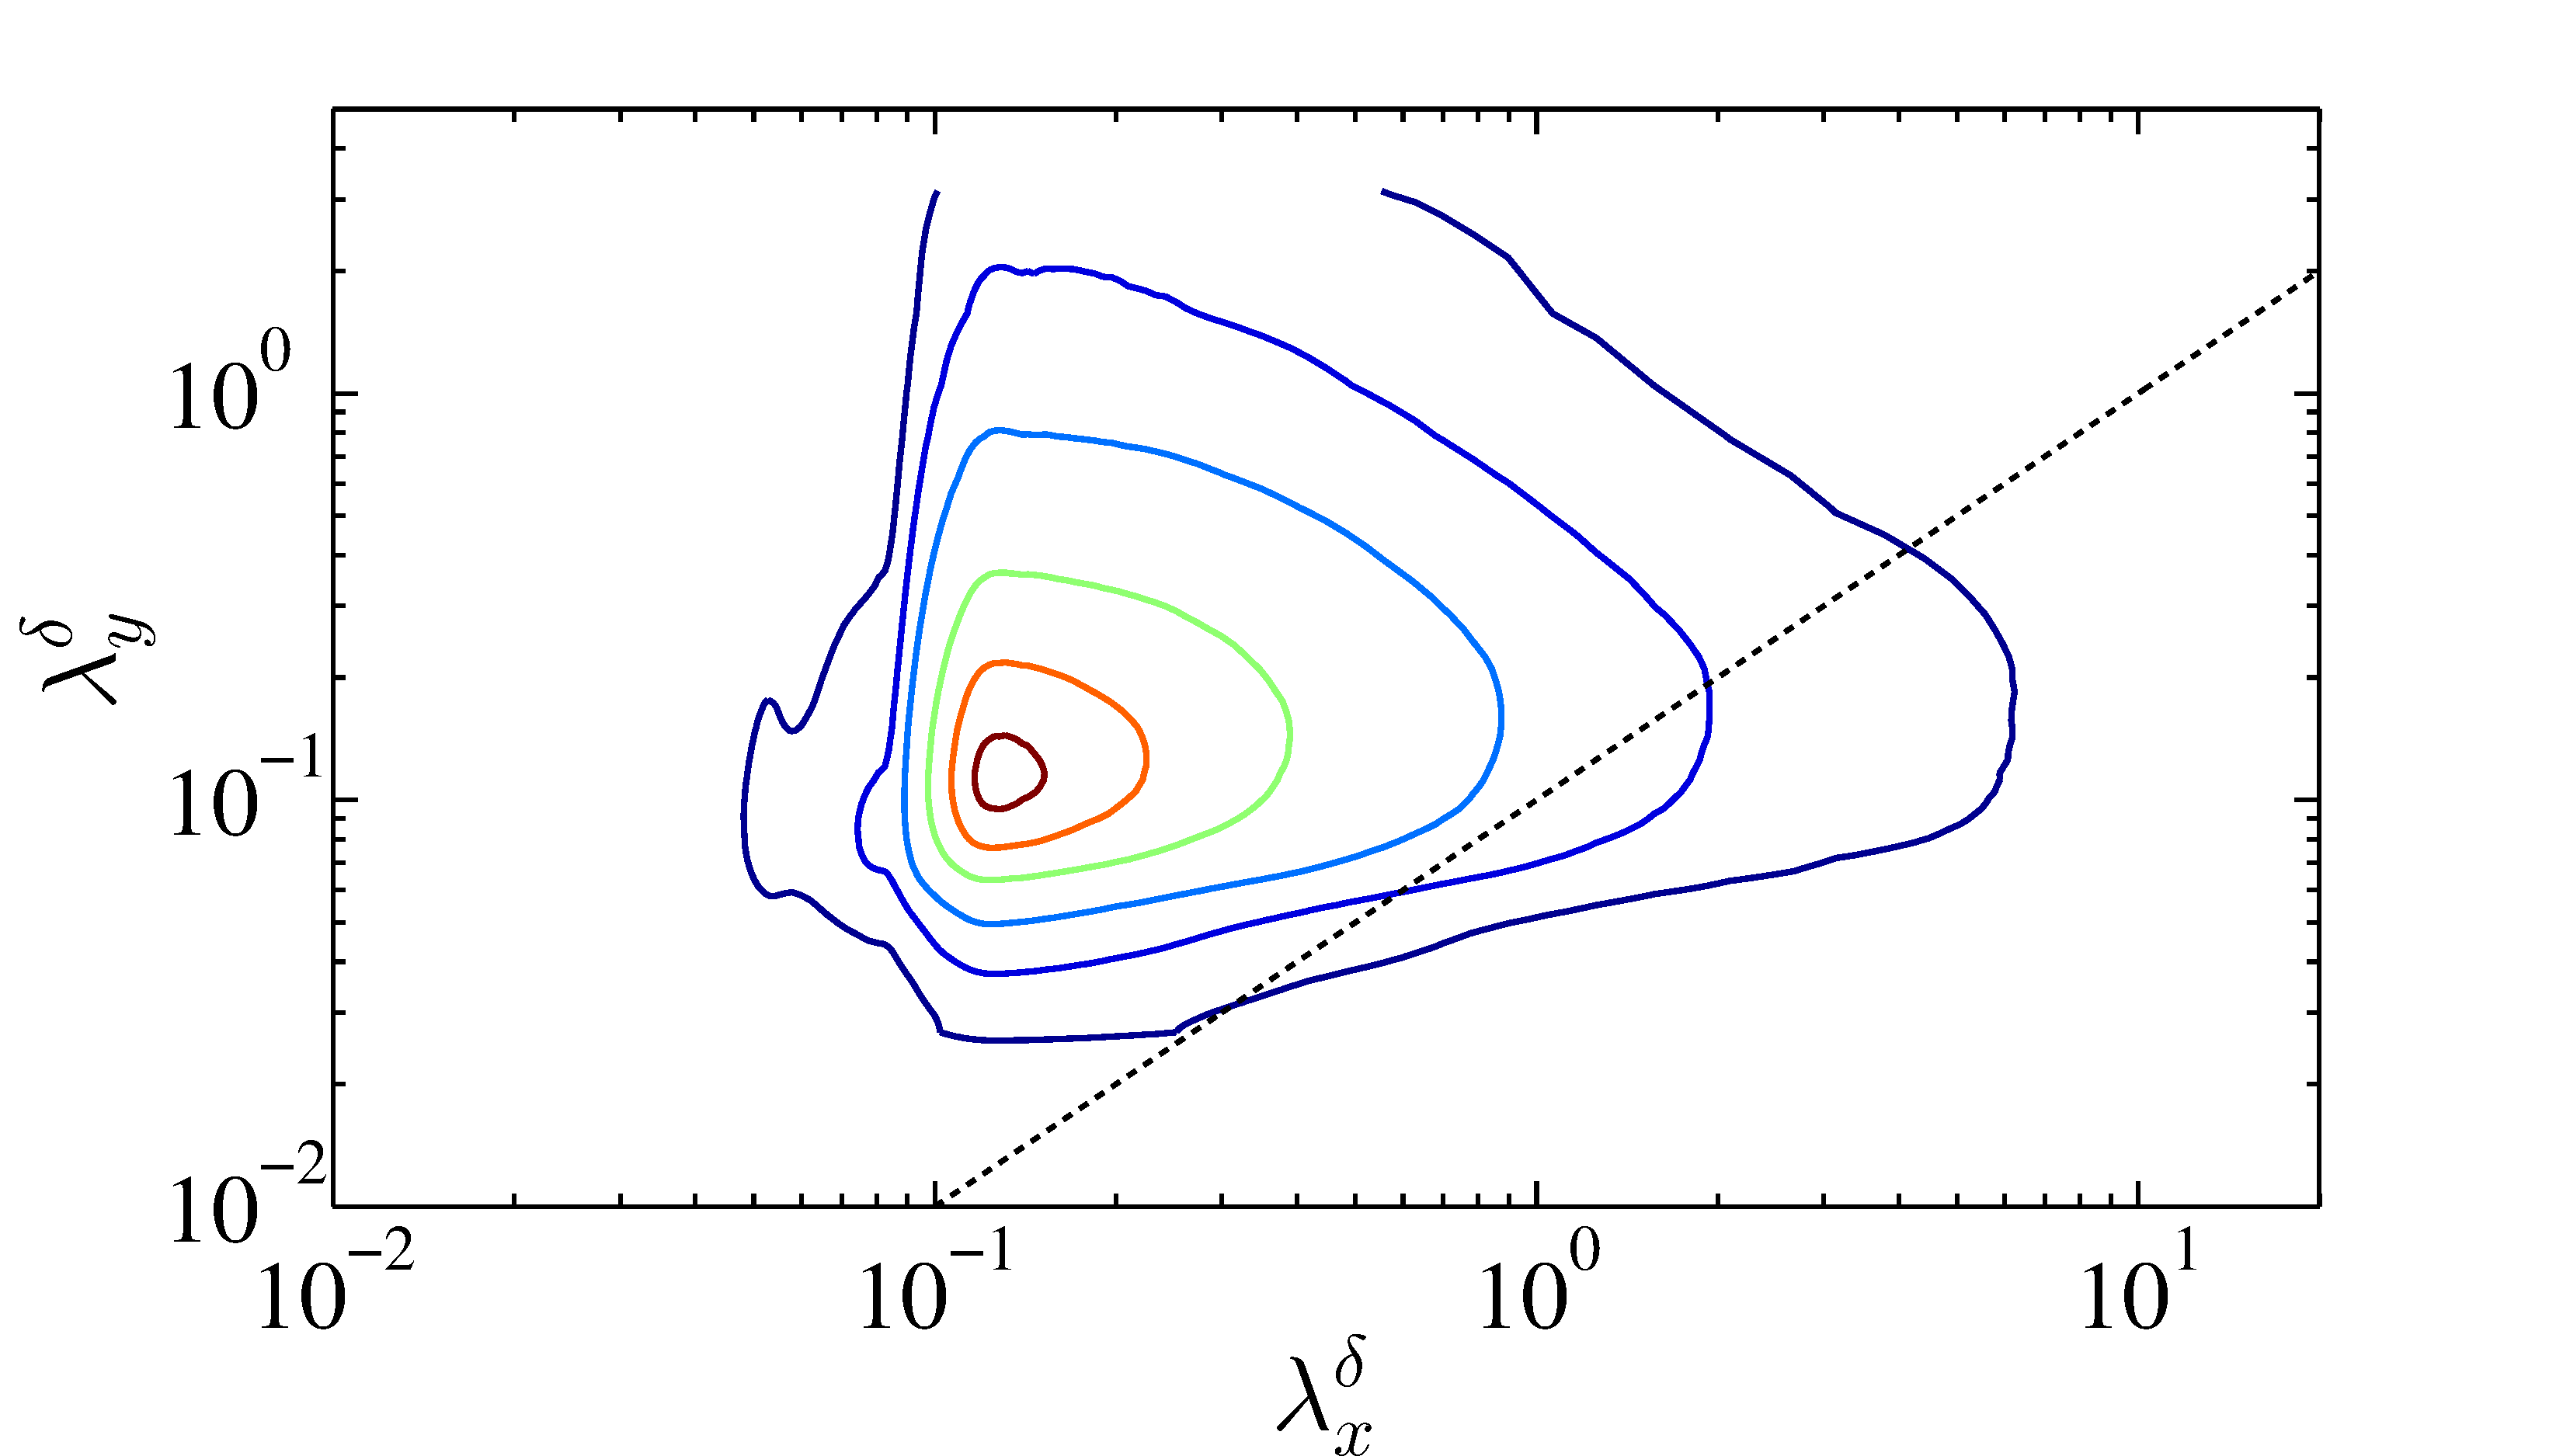
\includegraphics[width=\linewidth]{Fig2/dissp_contour_ABL_n05_filt2_level5.pdf}
                \caption{}
                \label{fig:dissip3}
        \end{subfigure}              
        
        \caption[Premultiplied Spectra 1]{2D Premultiplied spectra for Case IX ($\lbrace C_0 = 0.19, n = 0.5, k_c = 4\rbrace$) in the plane of normalized wavelengths $\lambda_x^{\delta}$ and $\lambda_y^{\delta}$, normalized by BL thickness $H$. Left: Streamwise energy spectra $k_xk_zE_{uu}(k_x,k_z)$, Right: Enstrophy spectra $k_xk_zE_{\omega\omega}(k_x,k_z)$, $(k_x, k_z)$: streamwise and spanwise wavenumbers respectively. (A)-(B) $z/H = 0.015$; (C)-(D) $z/H = 0.1$; (E)-(F) $z/H = 0.25$. Six contour levels are [0.05 0.125 0.25 0.5 0.75 0.95] times the maximum, with increasing from red to blue. Smallest enclosed contour is the maximum The dashed line represents $\lambda_x^{\delta} = 10 \lambda_y^{\delta}$}\label{fig:2d_spec_diss}
\end{figure}

\begin{figure}
\centering
        \begin{subfigure}[t]{0.5\textwidth}
                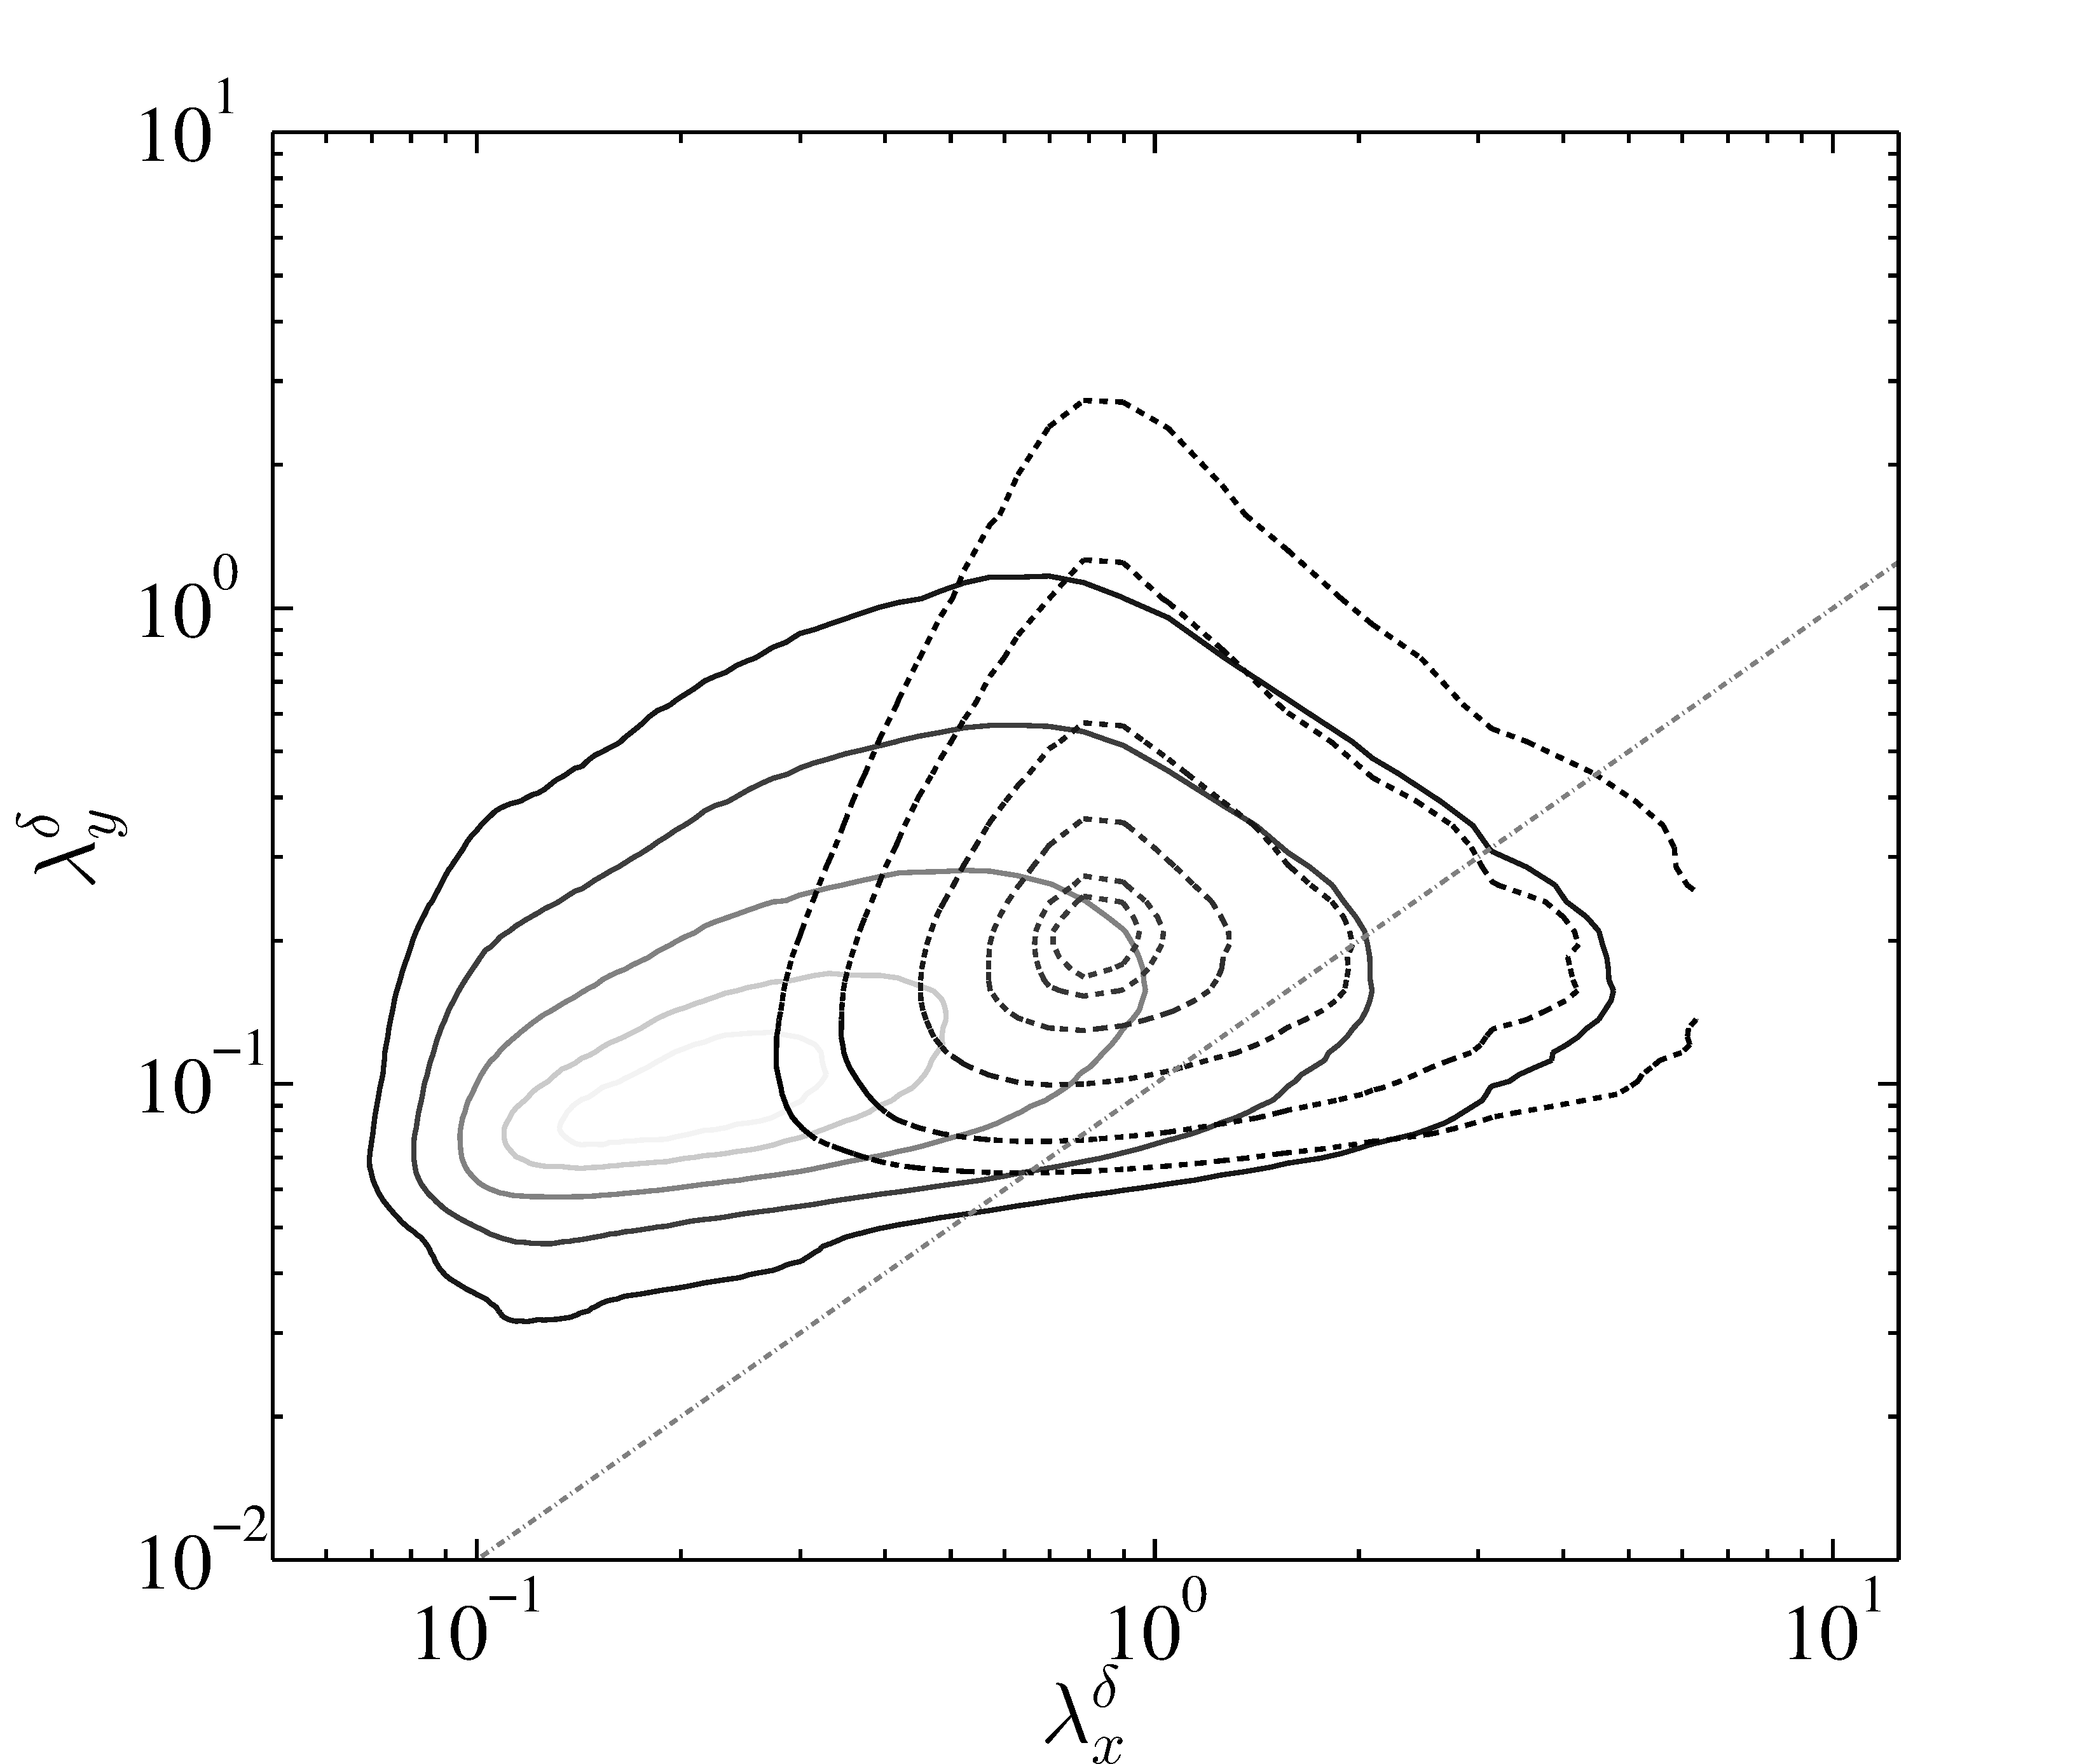
\includegraphics[width=\linewidth]{Fig3/energy_contour_ABL_n2n05_level2.pdf}
                \caption{}
                \label{fig:energy1b}
        \end{subfigure}%
        \centering
        \begin{subfigure}[t]{0.5\textwidth}
                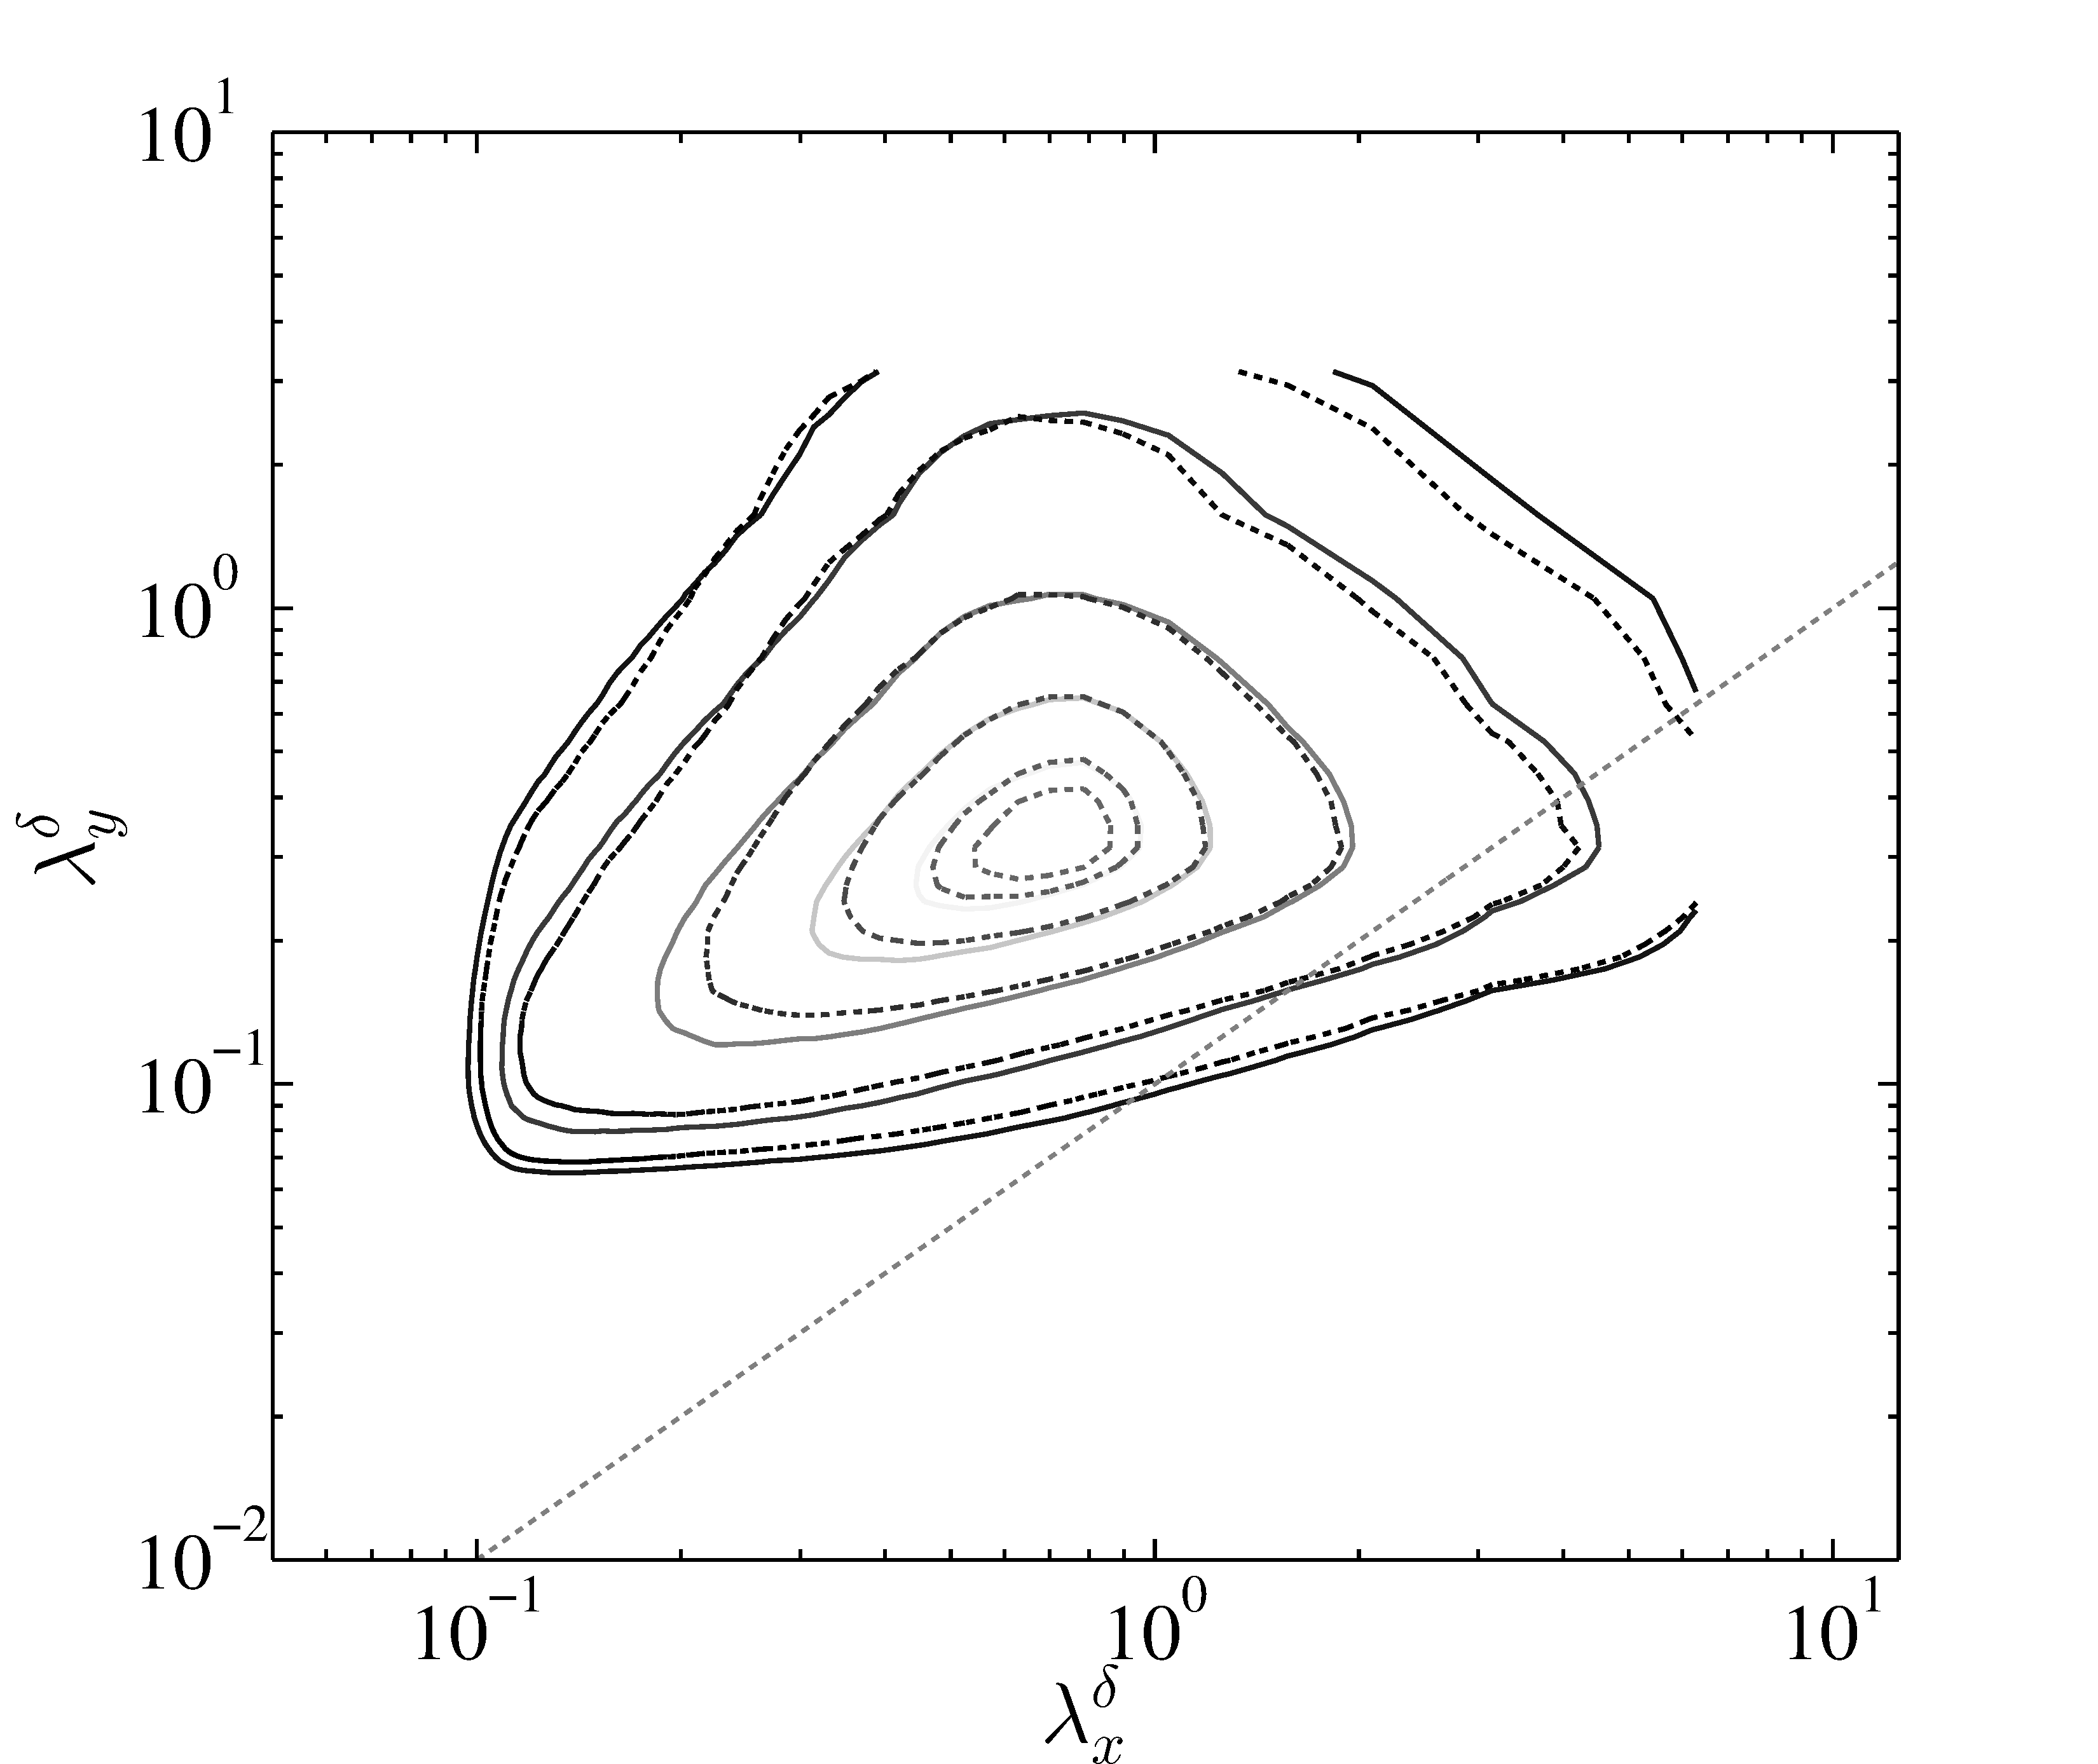
\includegraphics[width=\linewidth]{Fig3/energy_contour_ABL_n2n05_level5.pdf}
                \caption{}
                \label{fig:dissip1b}
        \end{subfigure}
\centering
        \begin{subfigure}[t]{0.5\textwidth}
                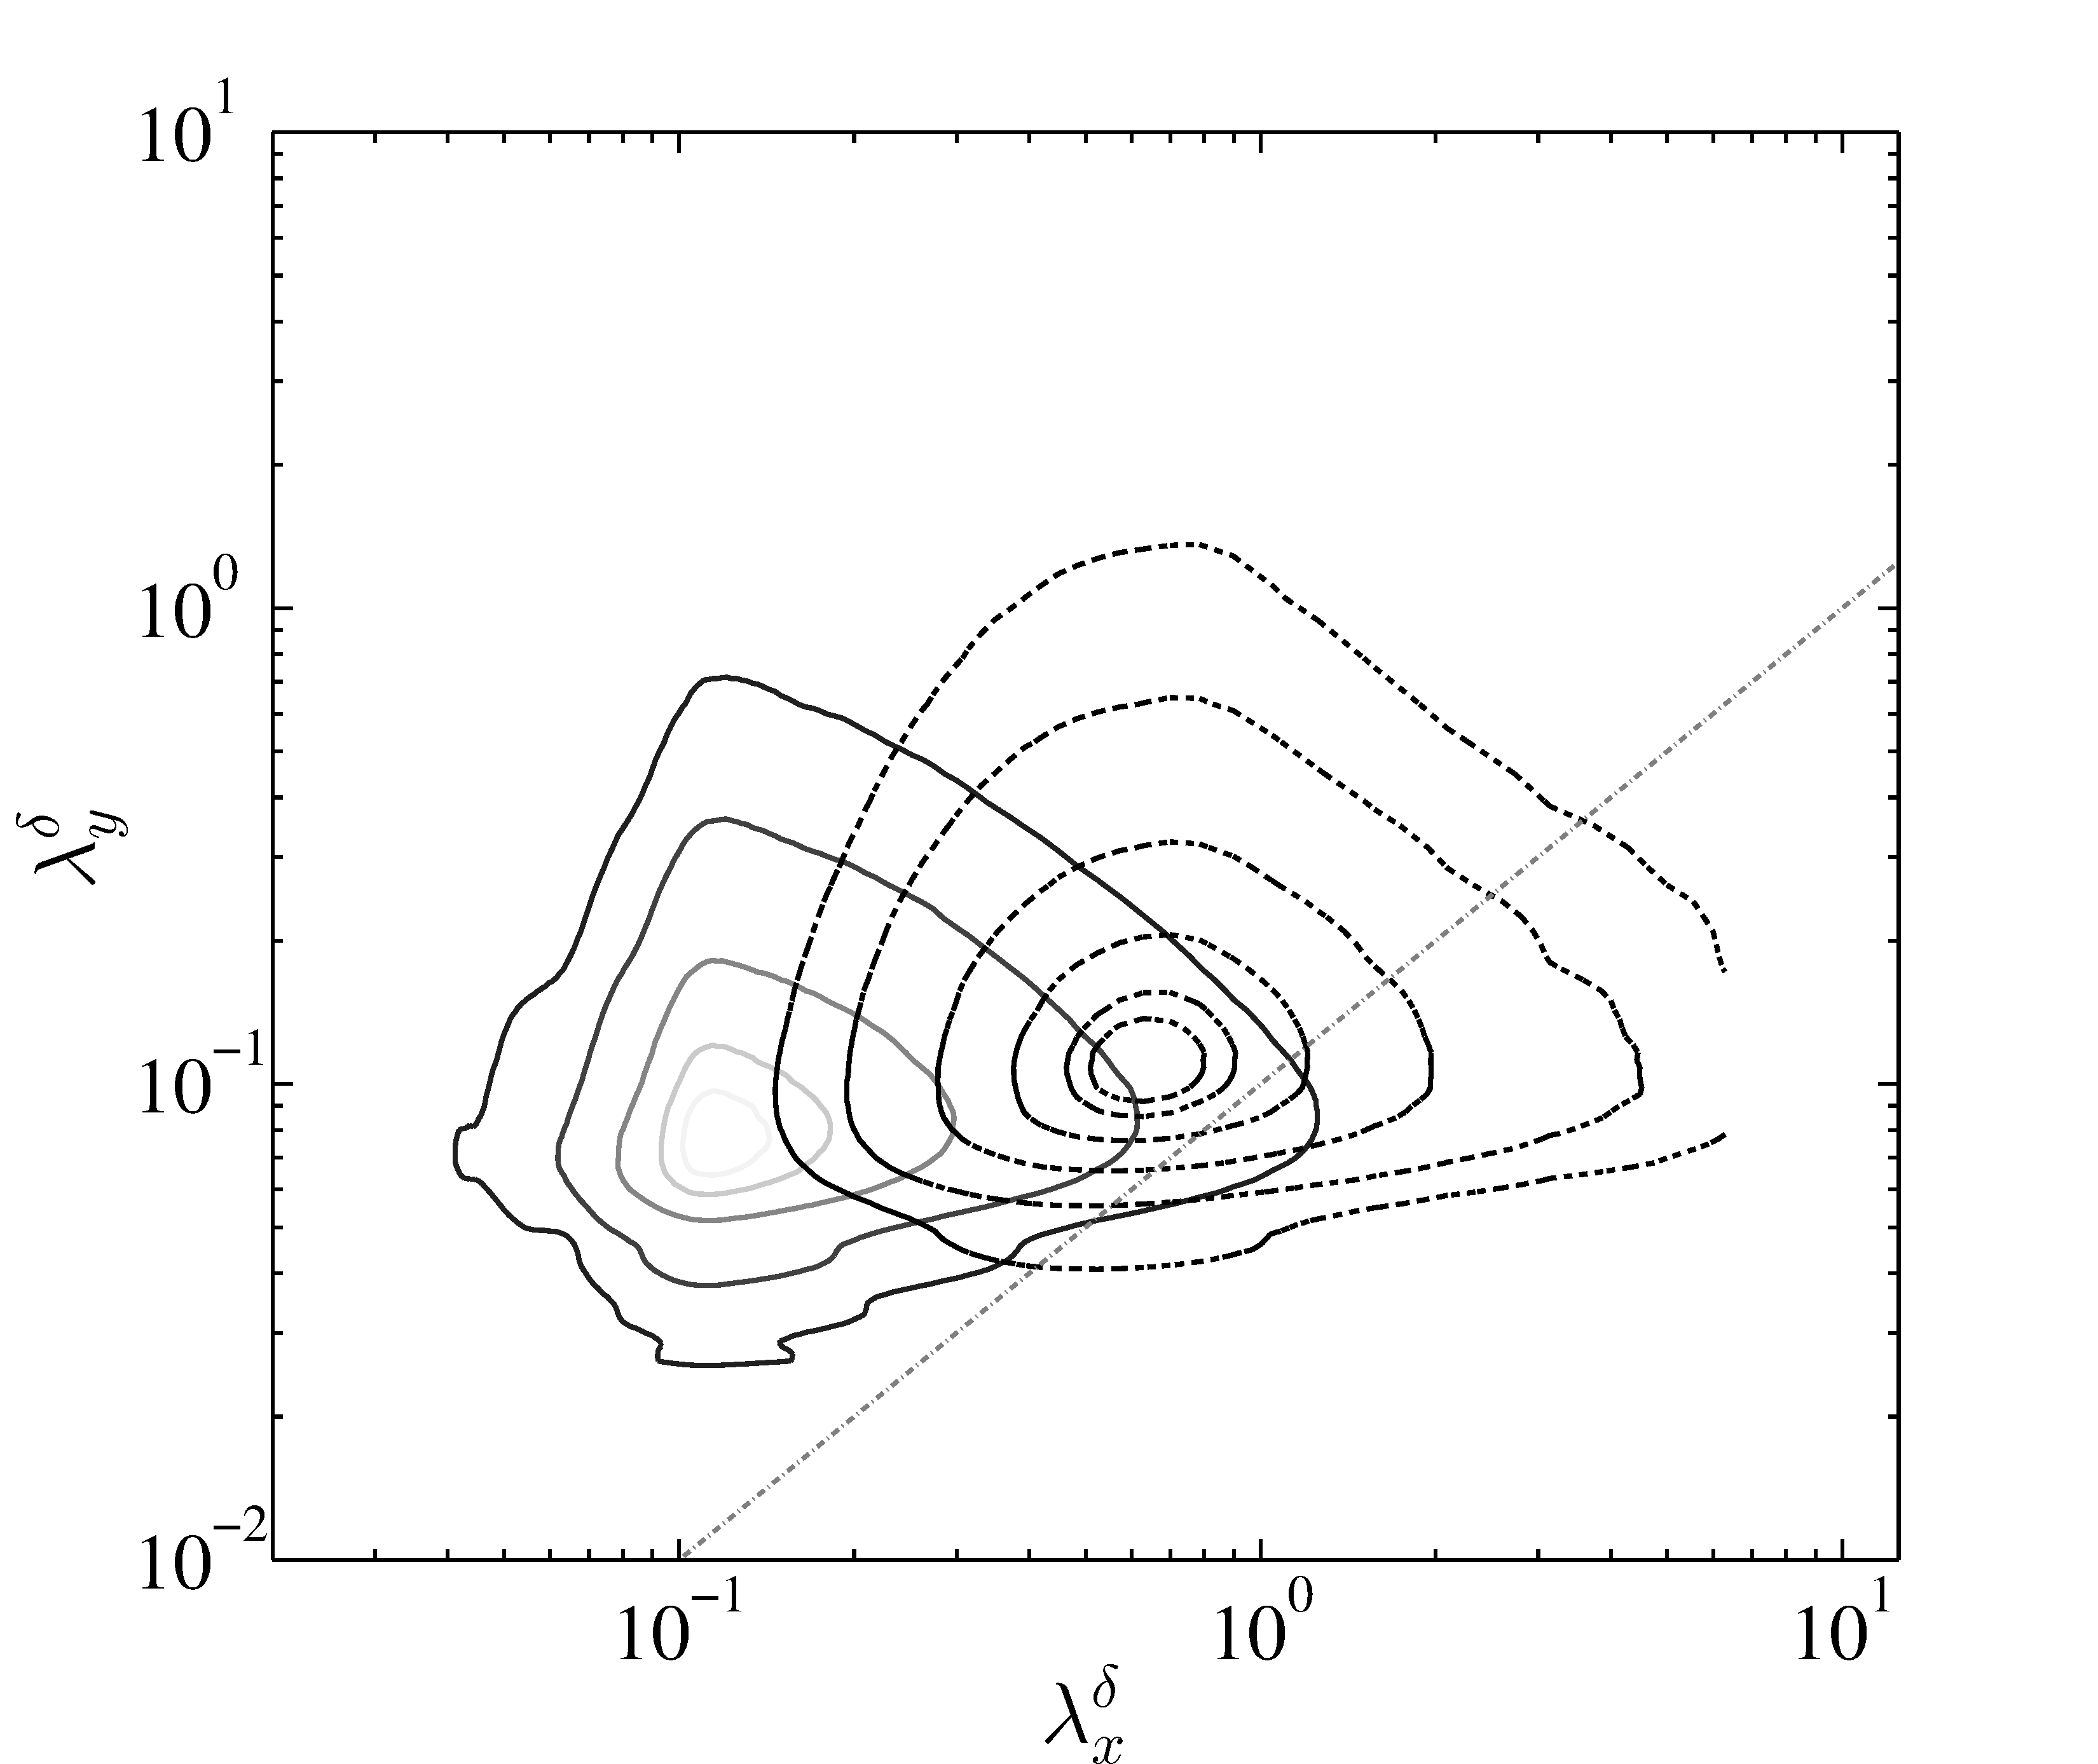
\includegraphics[width=\linewidth]{Fig3/dissp_contour_ABL_n2n05_level2.pdf}
                \caption{}
                \label{fig:energy2b}
        \end{subfigure}%
        \centering
        \begin{subfigure}[t]{0.5\textwidth}
                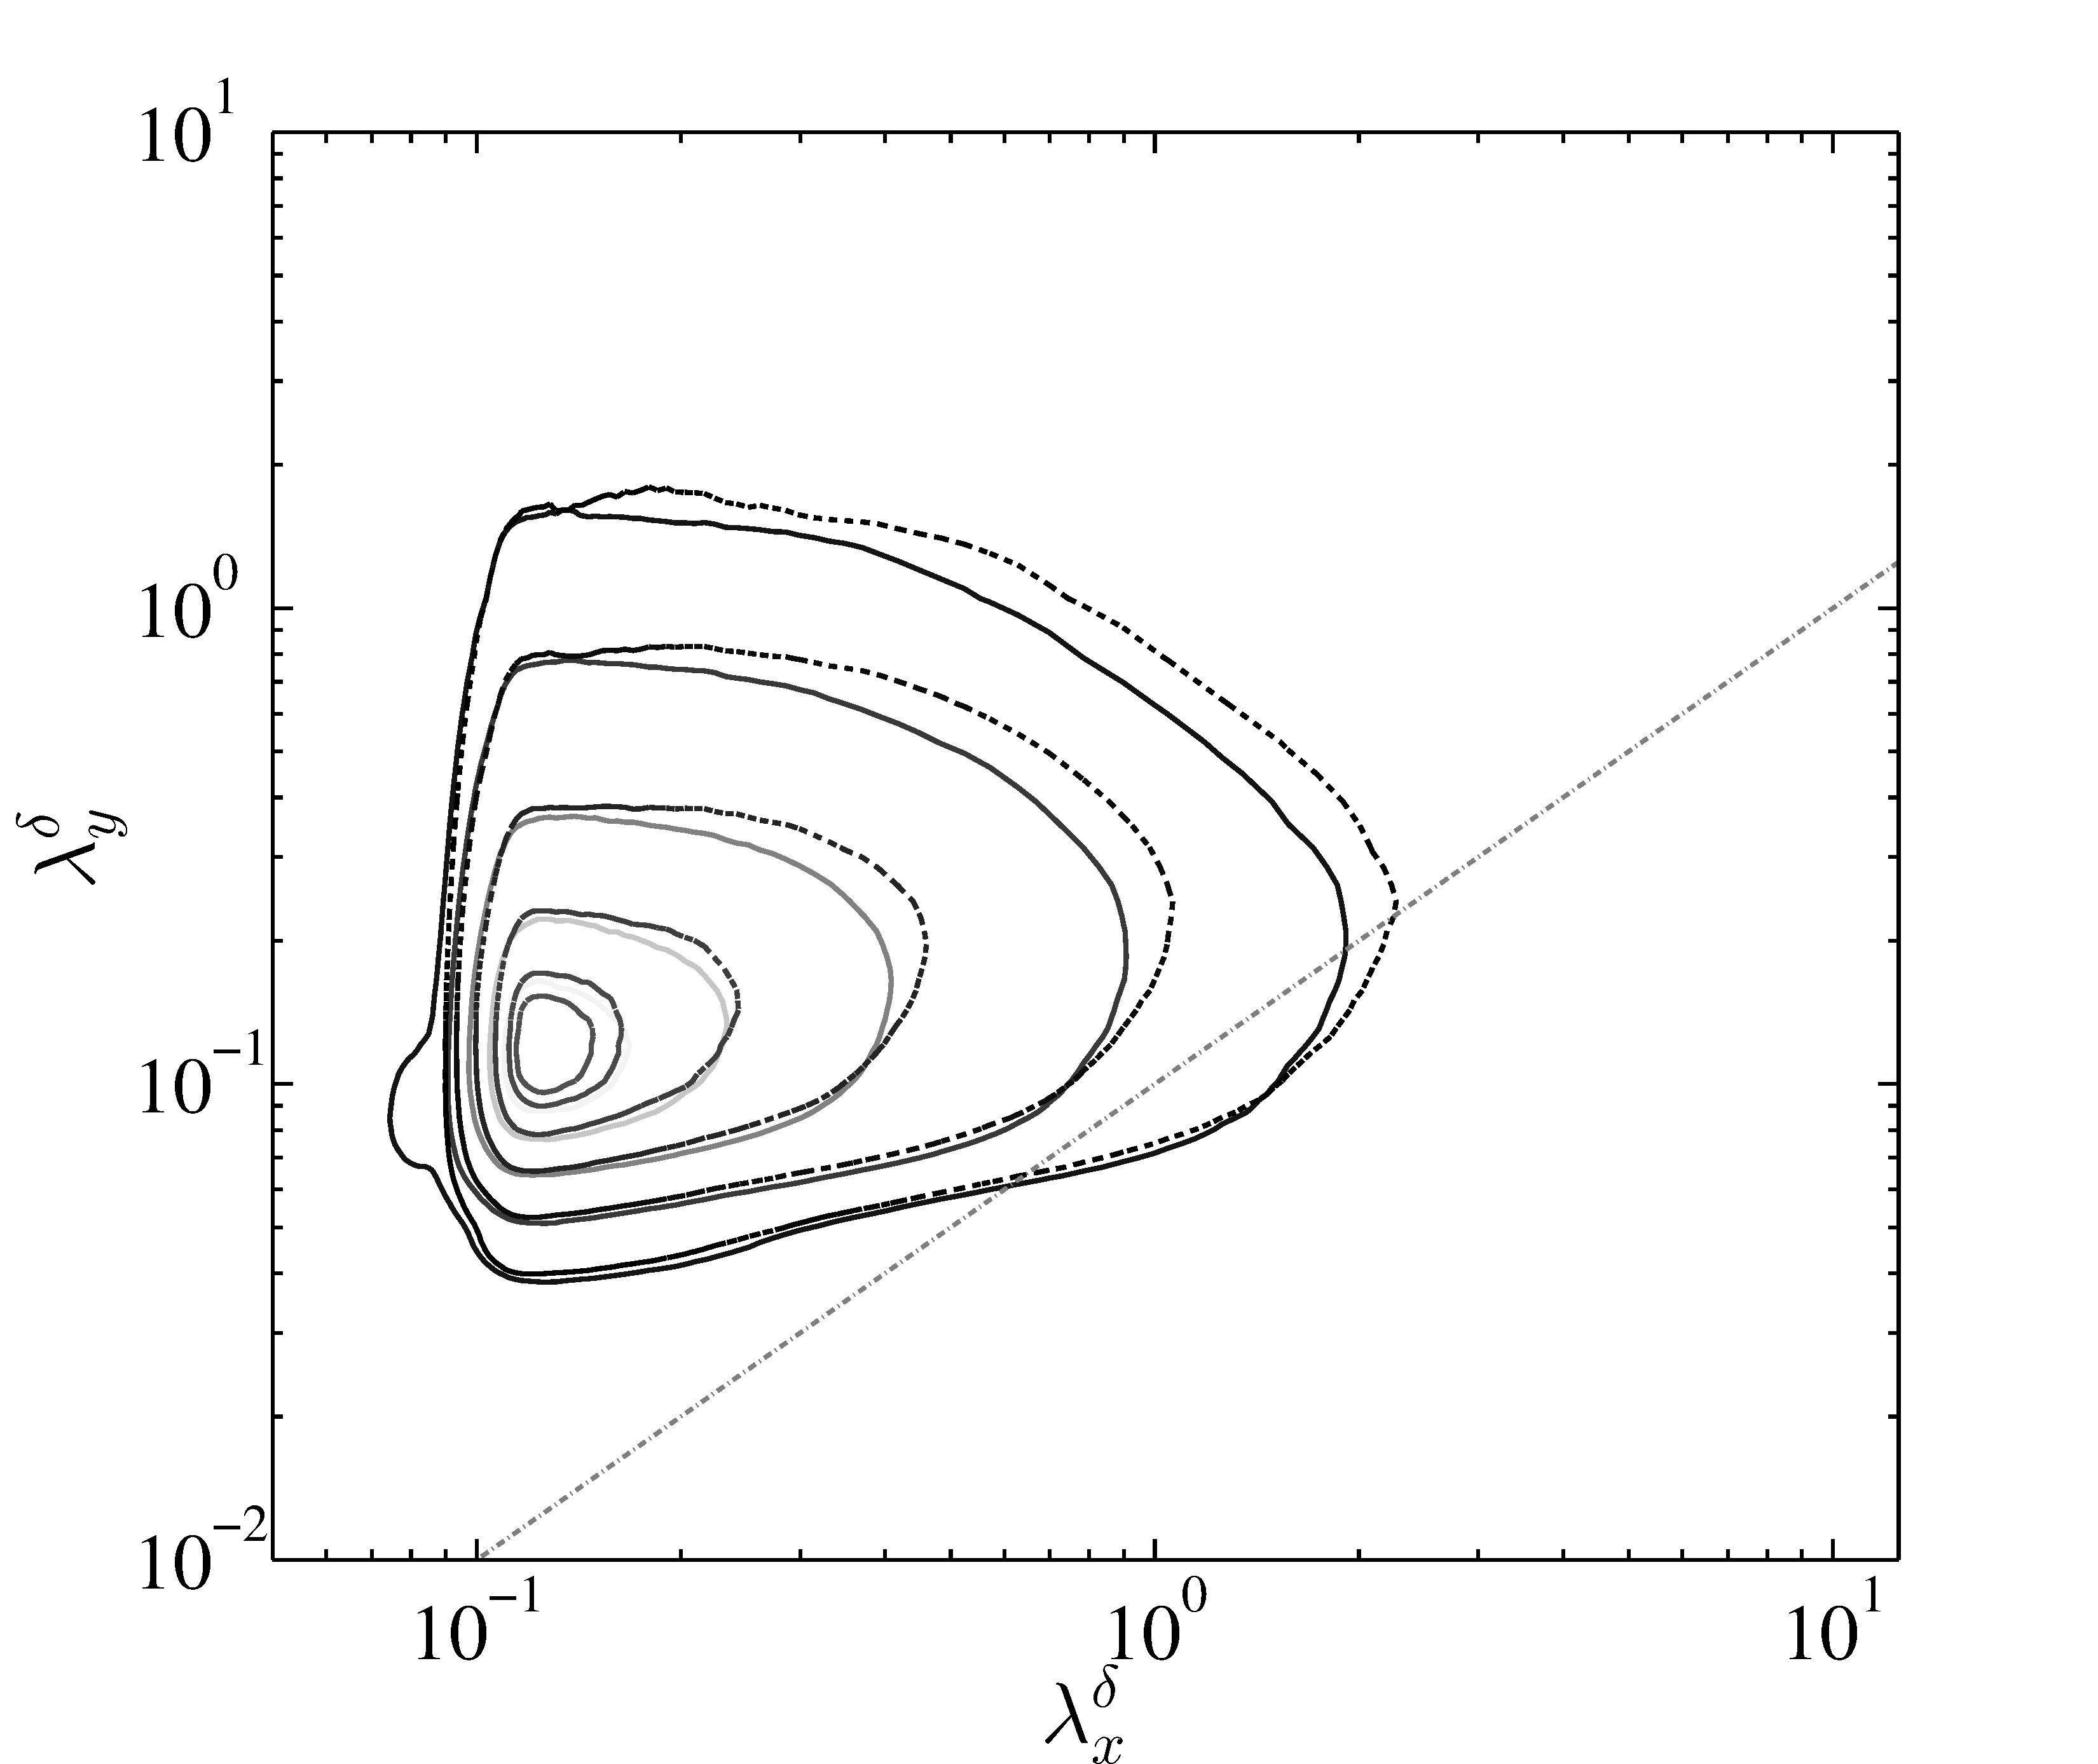
\includegraphics[width=\linewidth]{Fig3/dissp_contour_ABL_n2n05_level5.pdf}
                \caption{}
                \label{fig:dissip2b}
        \end{subfigure}
 \centering
        \begin{subfigure}[t]{0.5\textwidth}
                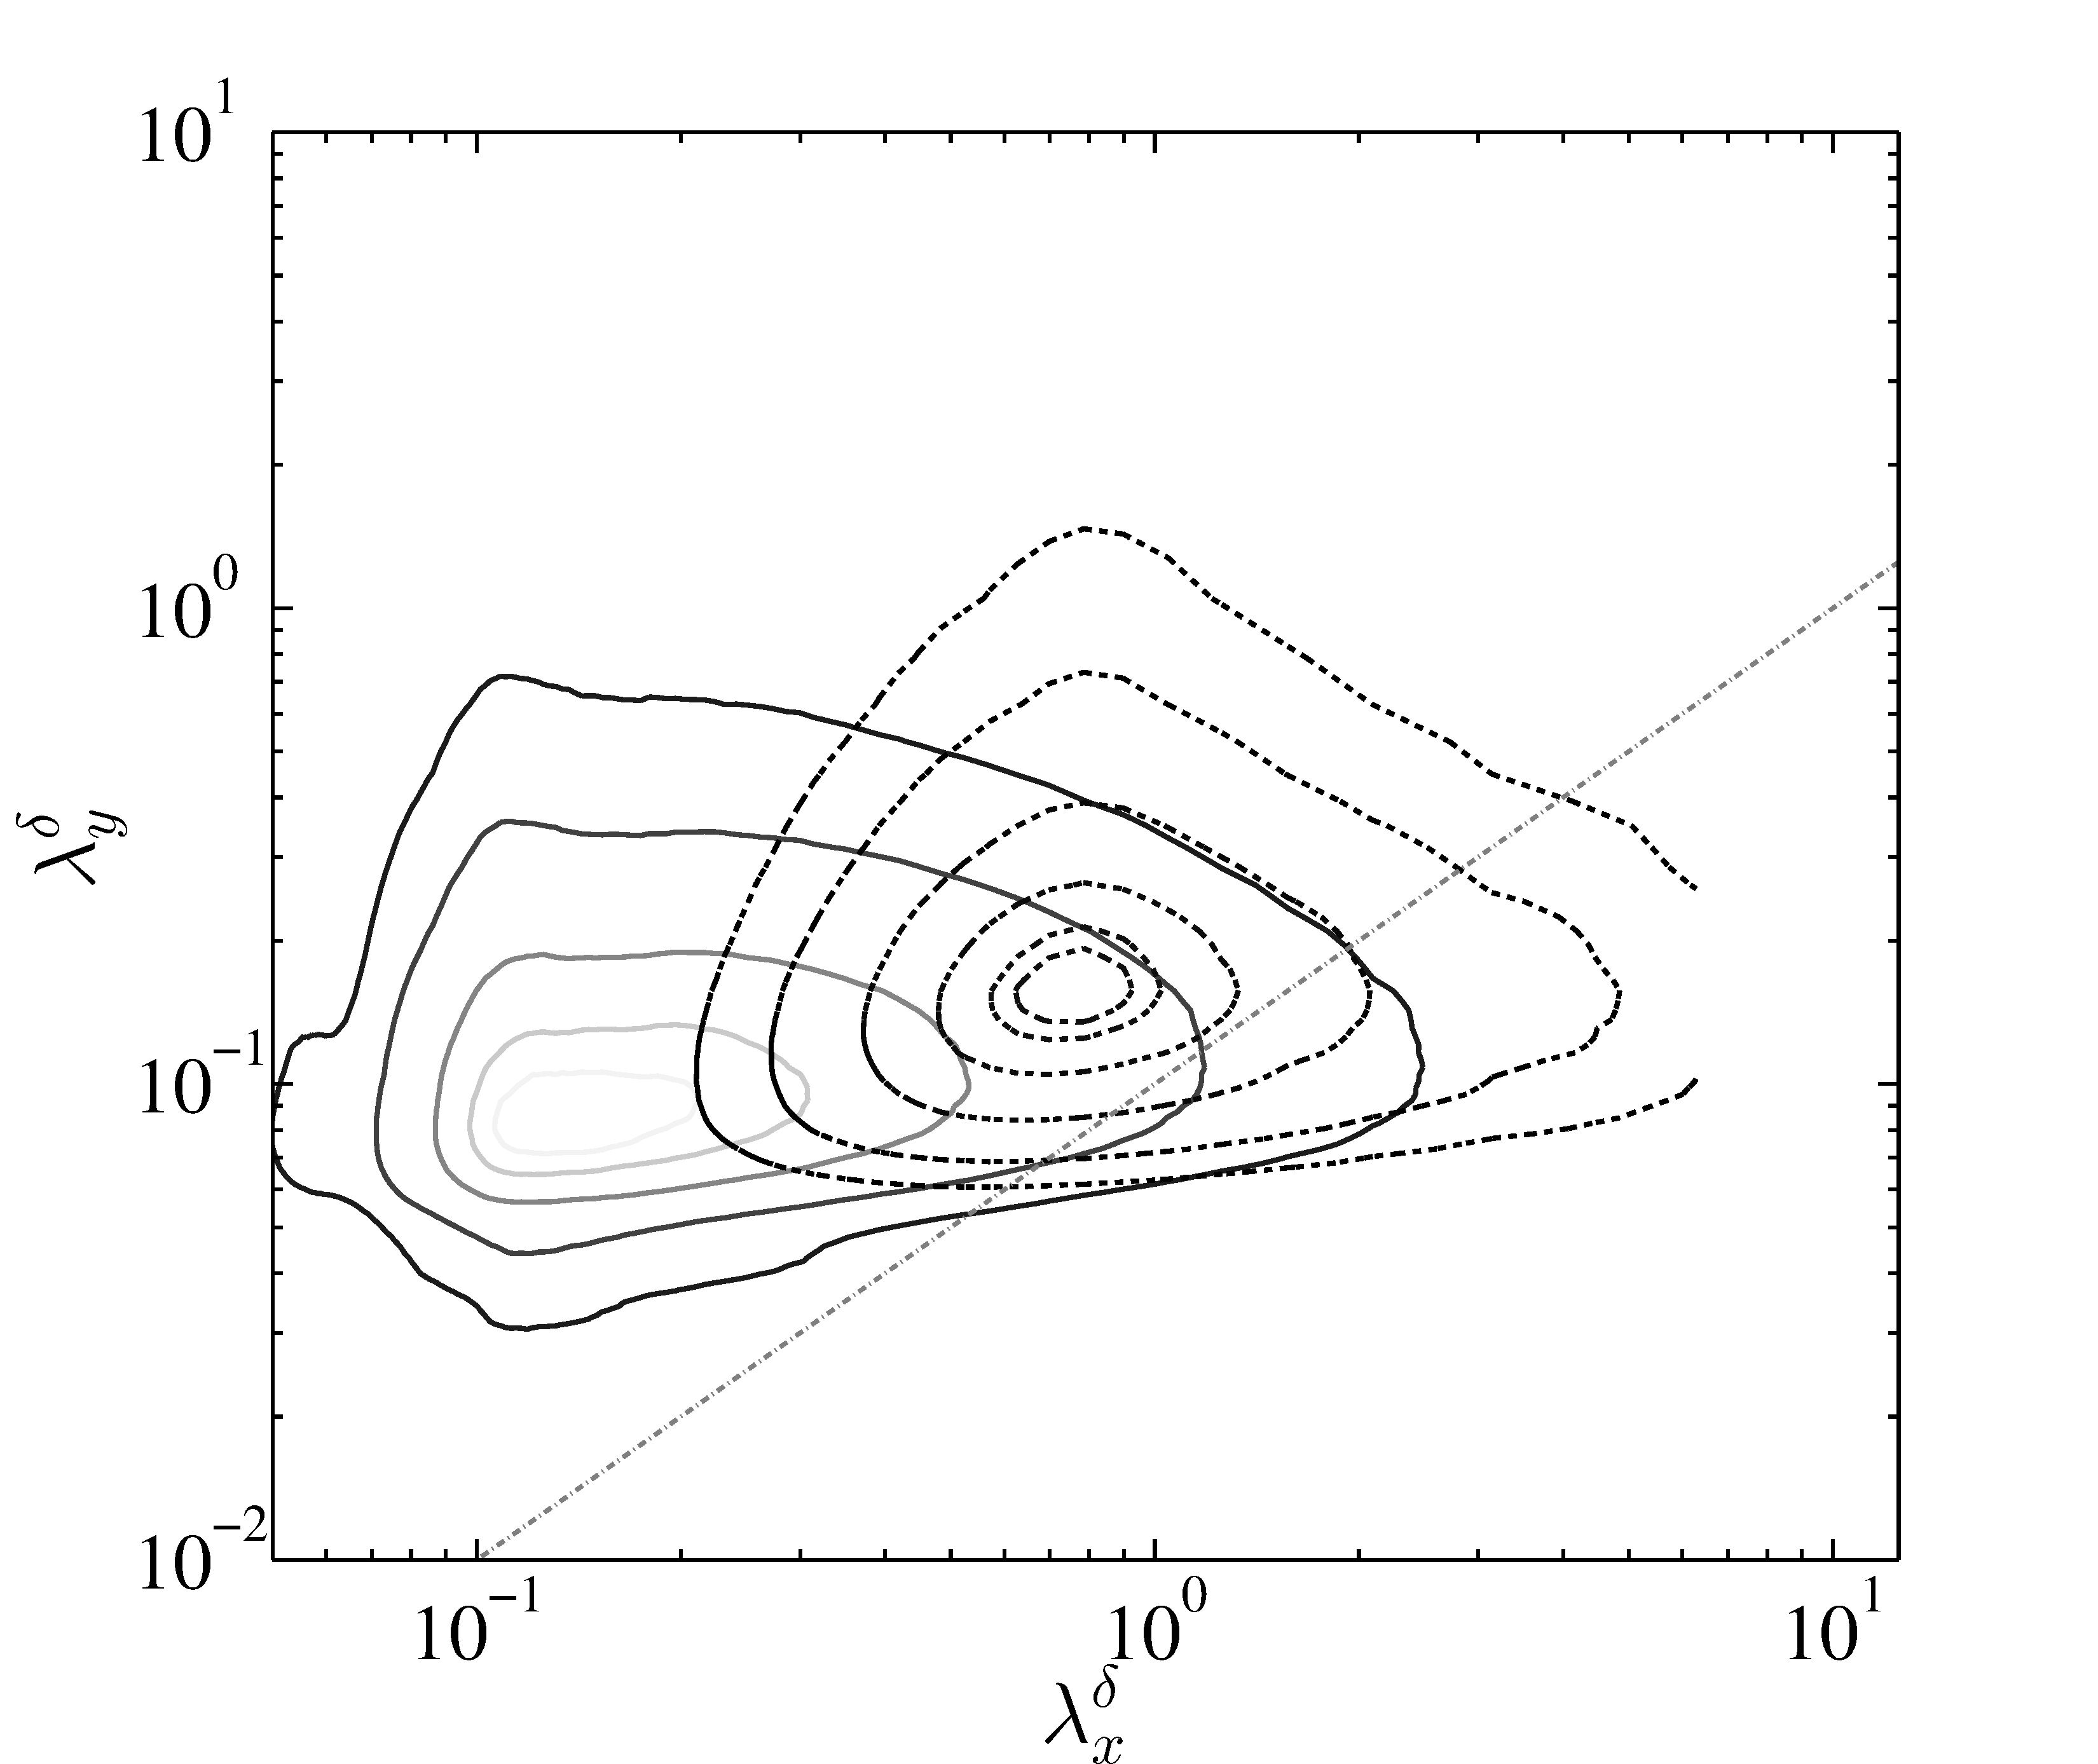
\includegraphics[width=\linewidth]{Fig3/cospectra_contour_ABL_n2n05_level2.pdf}
                \caption{}
                \label{fig:energy3b}
        \end{subfigure}%
        \centering
        \begin{subfigure}[t]{0.5\textwidth}
                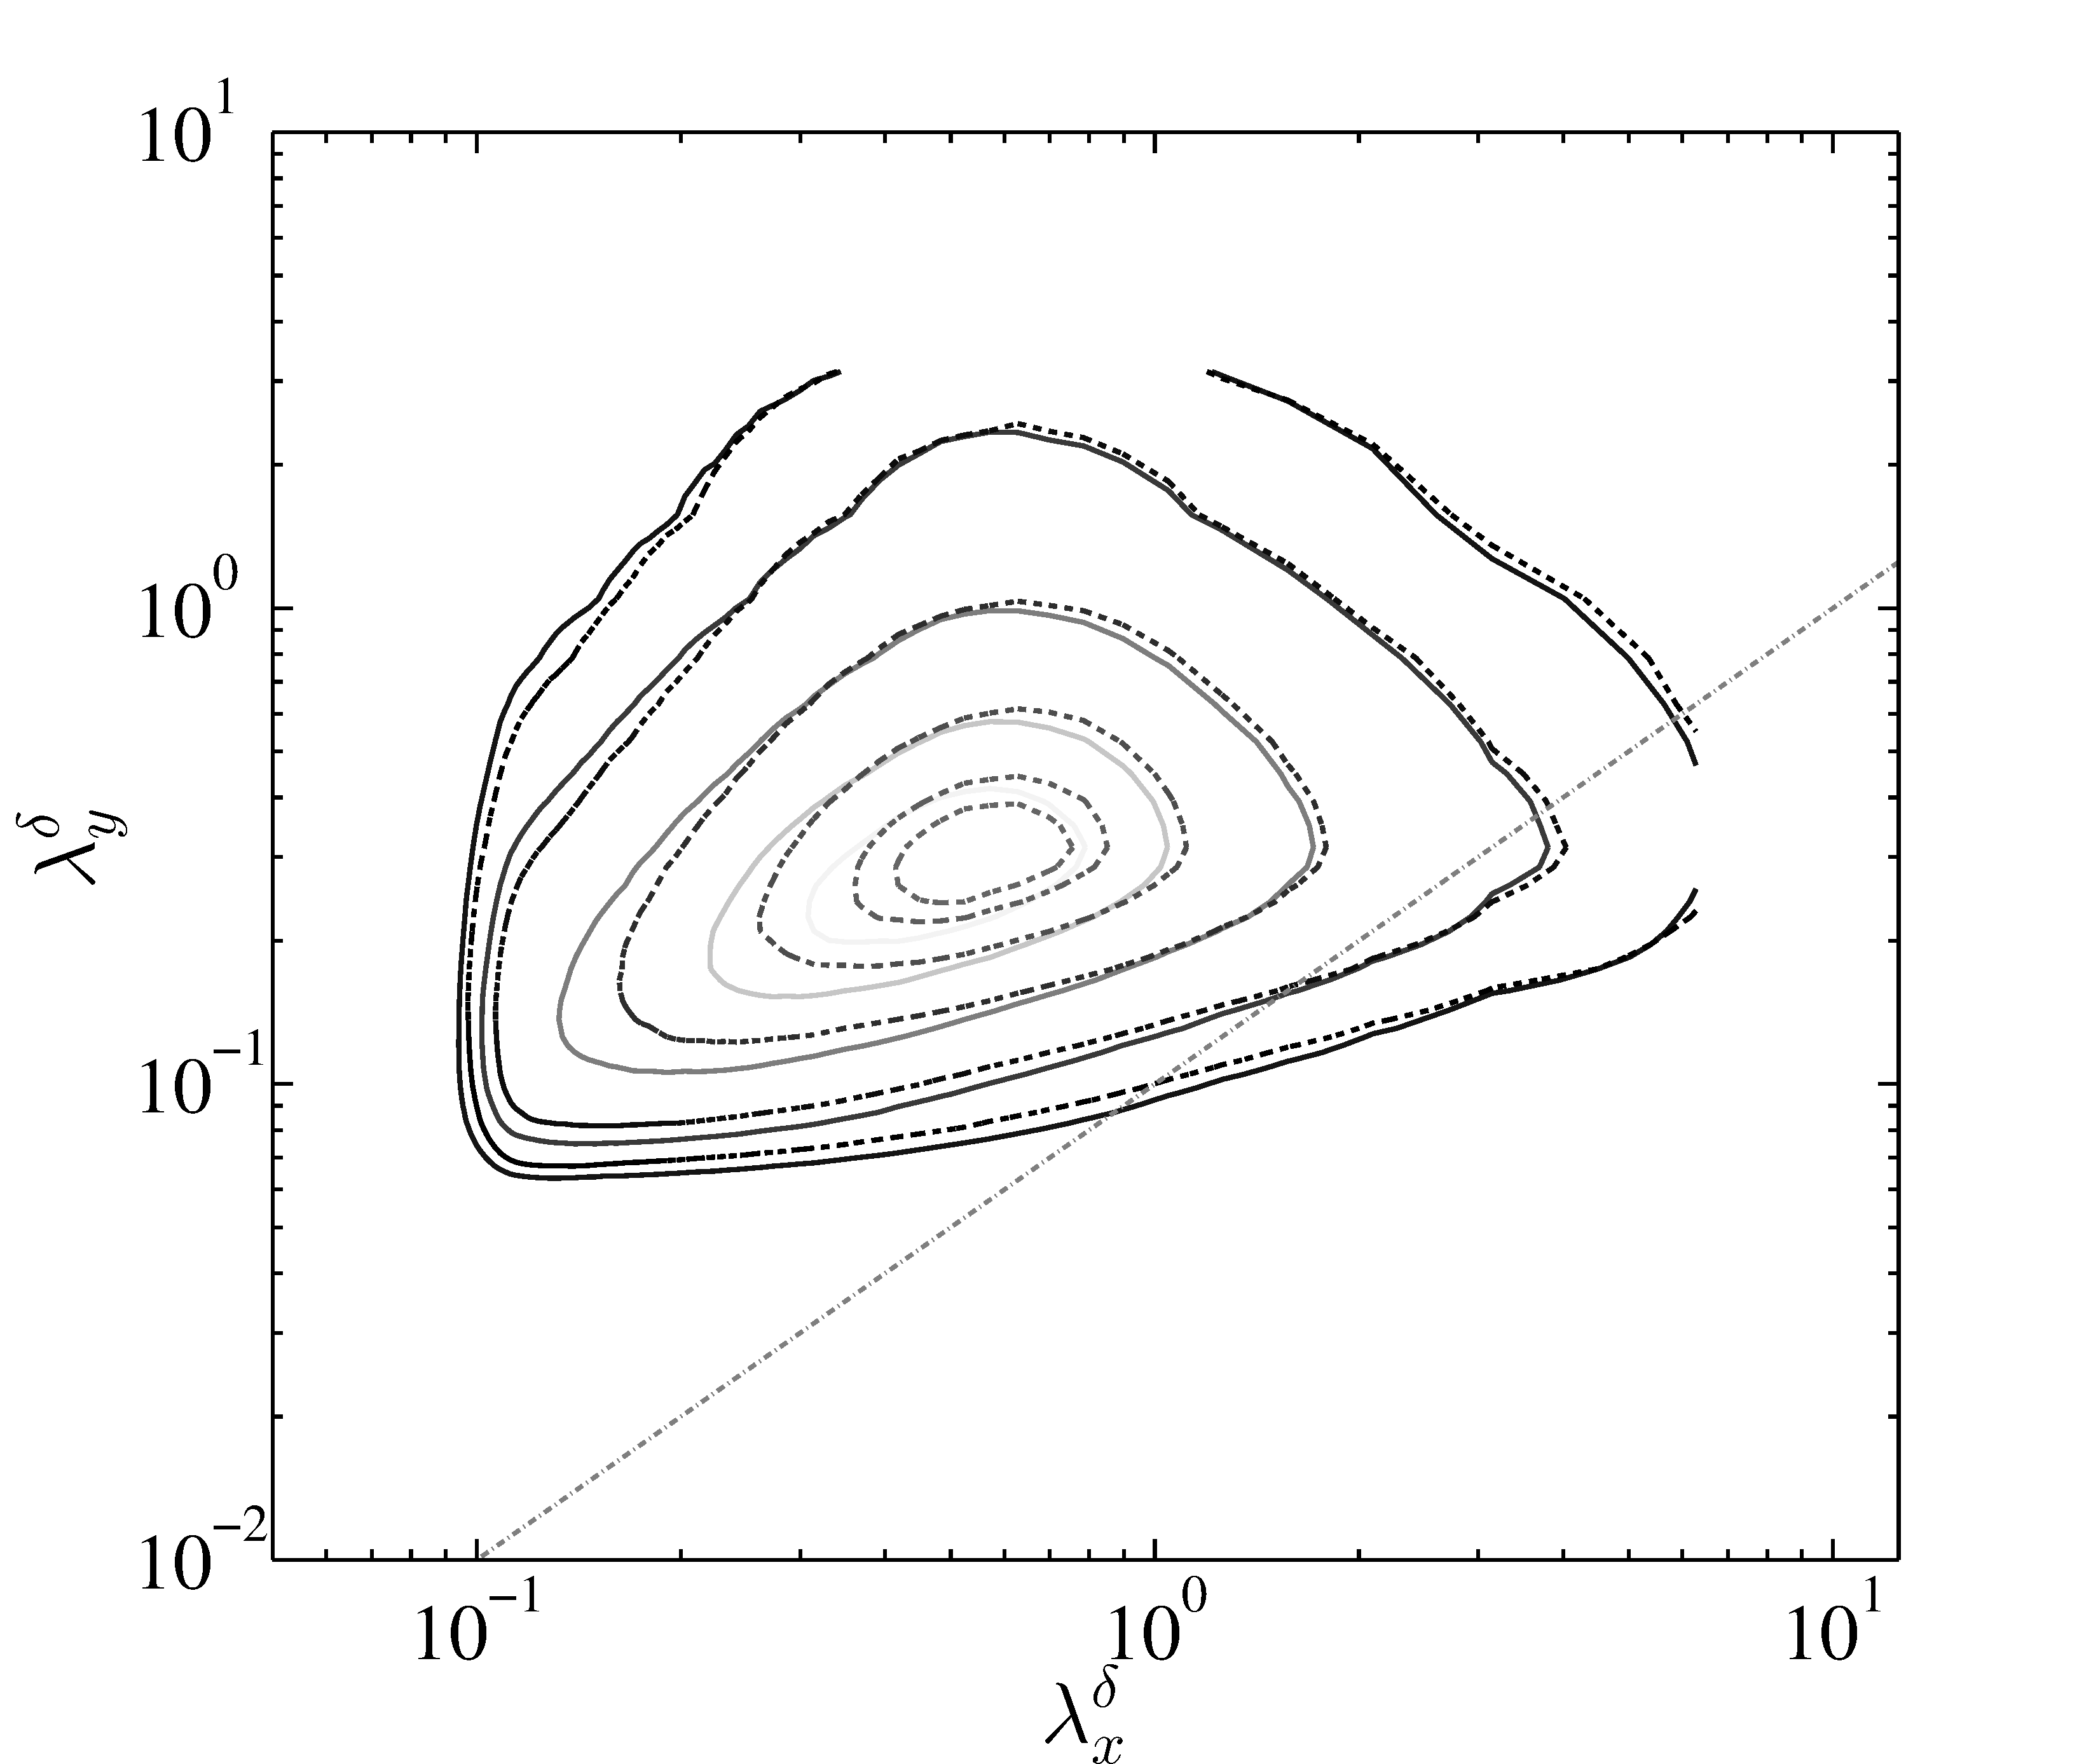
\includegraphics[width=\linewidth]{Fig3/cospectra_contour_ABL_n2n05_level5.pdf}
                \caption{}
                \label{fig:dissip3b}
        \end{subfigure}              
        
        \caption[Premultiplied Spectra 2]{2D Premultiplied spectra for comparing Cases II \& IX ($\lbrace C_0 = 0.16, n = 2, k_c = 4\rbrace$, $\lbrace C_0 = 0.19, n = 0.5, k_c = 4\rbrace$) in the plane of normalized wavelengths $\lambda_x^{\delta}$ and $\lambda_y^{\delta}$, normalized by BL thickness $H$. \textit{Left}: $z/H = 0.015$, \textit{Right}: $z/H = 0.25$ (A)-(B), Energy Spectra $k_xk_zE_{uu}(k_x,k_z)$, (C)-(D) Surrogate of dissipation or Enstrophy spectra $k_xk_zE_{\omega\omega}(k_x,k_z)$ and (E)-(F) Cospectra of Reynolds shear stress $k_xk_z\phi_{uw}(k_x,k_z)$. Solid contours: Case II, Dashed contours: Case IX. From ligher grey to dark is increasing contour levels. [0.125 0.25 0.5 0.75 0.9 0.95] times the maximum. Smallest enclosed contour is the maximum. The dashed line in each plot represents $\lambda_x^{\delta} = 10 \lambda_y^{\delta}$} \label{fig:2d_spec_diss2}
\end{figure}

\subsection{Low Dissipation trends with $n = \frac{1}{2}$}
The low (and also physically consistent) dissipative nature of the standard Smagorinsky model with Mason and Thompson~\cite{mason} wall damping using $n = \frac{1}{2}$ can be further corroborated in the Figures~\ref{fig:grad1},~\ref{fig:shear1},~\ref{fig:spec},~\ref{fig:highdiff},~\ref{fig:lowdiff}
.{Figure~\ref{fig:grad1} is an effortless manifestation of the reduction of ``log-layer mismatch" with $n = \frac{1}{2}$. All the plots in the Figure~\ref{fig:grad1} are with $k_c = 2$.}  \\
In Figure~\ref{fig:shear1}, the symbol plots refer to the relative error of near wall mixing length $l_m = {u_{\tau}}{f(z)/\langle\vert \widetilde{S} \vert\rangle_{xy}}$ \textcolor{red}{did you ever define $l_m$ that way?} (lengthscale of near-wall eddies) with that of the ideal $\kappa z$ near log-layer shown by the solid black line. Figure~\ref{fig:shear1} clearly shows that with $n = \frac{1}{2}$ (black $\circ$), the error in the mixing length decreases significantly compared to the other plots using $n = 1$ {that} saturate to $100\%$ error at $z/H \gtrapprox 0.05$. It is also observed that when $n = 1$, even by decreasing {$C_0$} to 0.13, the $l_m$ error does not reduce indicating {that} the persistence of ``log-layer mismatch" is directly correlated with the shape of $C_s$ and not just its magnitude.

The streamwise energy spectra for $n = 2$ and $n = \frac{1}{2}$ are shown in Figures~\ref{fig:stat0_lotw2},~\ref{fig:stat0_lotw3}. The spectra normalized with $u_{\tau}, z$ consistently reveals the two spectral ``overlap regions", $k_1^{-1}$ and $k_1^{-{5}/{3}}$ laws,~\cite{perry,porte1fun,meyers2} where $k_1$ is the streamwise wavenumber (in the contour plots of premultiplied spectra in Figures~\ref{fig:2d_spec_diss},~\ref{fig:2d_spec_diss2} we refer to $k_x$ as the streamwise wavenumber which really is $k_1$), with the change of slope near $k_1 z \sim 1 $. At $z/H = 0.5$ (outer layer) the energy spectrum of both $n = 2$ and $n = \frac{1}{2}$ are quite a good match and show a drop in the energy spectrum at approximately the same region $k_1 z \sim O(10)$.  However, at log-layer ($z/H = 0.1$), the spectrum shows {deviation from the expected slope} at {$k_1 z \sim O(1)$} for $n = 2$, whilst for $n = \frac{1}{2}$, the {deviation} occurs at {significantly higher values of $k_z$ close to $\sim O(10)$} indicating that the effects of dissipation on smaller scales near wall are more conspicuous with $n = 2$. Also, for $n = 0.5$, the normalized spectra collapses into a single curve in the $-5/3$ law region which is expected from the scaling laws~\cite{perry}. This is further corroborated in Figure~\ref{fig:vort}, where more structures of near wall $x$ vorticity can be observed with $n = 0.5$ than with $n = 2$.

\subsubsection{Premultiplied Spectra: understanding dissipation trends}
The two dimensional streamwise energy spectra spectra in wavenumber plane ($\lambda_x, \lambda_z$), at a particular wall normal location $z/H$, can be given as $E_{uu}(k_x,k_z)$. The total temporally averaged streamwise kinetic energy $E_{u,z}$ at that wall normal location can be given by
\begin{equation}
E_{u,z} = \int_{0}^{k_x}\int_{0}^{k_z}E_{uu}(k_x,k_z)\mathrm{d}k_x\mathrm{d}k_z \label{eq:spectra}
\end{equation}
When we plot the spectra in logarithmic scale we can manipulate Equation(~\ref{eq:spectra}) to obtain
 \begin{equation}
E_{u,z} = \int_{0}^{k_x}\int_{0}^{k_z}k_xk_zE_{uu}(k_x,k_z)\frac{\mathrm{d}k_x}{k_x}\frac{\mathrm{d}k_z}{k_z} = \int_{0}^{k_x}\int_{0}^{k_z}k_xk_zE_{uu}(k_x,k_z)\mathrm{d}(\log k_x)\mathrm{d}(\log k_z) \label{eq:spectra2}
\end{equation}
Thus the advantage of using pre multiplied spectra in logscale is that it essentially displays the energy content at respective scales and at the same time can project information on wider range of scales. Along the same lines we can design the premultiplied enstrophy spectra $k_xk_zE_{\omega\omega}(k_x,k_z)$ , where enstrophy is essentially a surrogate of dissipation (containing product of gradients, and enstrophy is essentially product of vorticity directly related to gradients) and premultiplied co-spectra $k_xk_z\phi_{uw}(k_x,k_z)$ of the kinematic shear stress which play a pivotal role in turbulence production.
\begin{eqnarray}
E_{\omega,z} & = &  \int_{0}^{k_x}\int_{0}^{k_z}k_xk_zE_{\omega\omega}(k_x,k_z)\mathrm{d}(\log k_x)\mathrm{d}(\log k_z) \\
-\overline{u'w'}(z) & = & -\int_{0}^{k_x}\int_{0}^{k_z}k_xk_z\phi_{uw}(k_x,k_z)\mathrm{d}(\log k_x)\mathrm{d}(\log k_z)
\end{eqnarray}
It is thus quite straightforward to understand that these premultiplied spectra is a very powerful tool in suggesting the nature (how anisotropic are they) and structure (streamwise and spanwise length scales) of the energy containing/turbulence producing and dissipative eddies. The premultiplied spectra can also used effectively to understand tthe structural information of the near wall ``active" eddies which play a significant role in producing turbulent shear stresses and turbulent kinetic energy along the lines of the classic attached-eddy hypothesis of Townsend~\cite{town1,town2} and later extended and verified by other researchers~\cite{perry,balad,jimrev}.\\
The contour plots in Figures~\ref{fig:2d_spec_diss},~\ref{fig:2d_spec_diss2}, shows that using different values of $n$ actually registers the difference in the eddy structures in the near-wall region with the log law ($z/H = 0.015$) while not significant differences can be seen in outer layer $z/H = 0.25$. With $n = 1/2$ we observe strong and consistent anisotropy in the energetic and high kinematic shear stress containing scales with $\lambda_x \approx 10\lambda_z$ (See Figures~\ref{fig:2d_spec_diss2}) which is consistently supported in previous literature containing DNS studies~\cite{hoyas,jimrev}. However, this anisotropy is absent in the near wall region when $n = 2$ is being used, depicting smearing of scales due to unphysical over dissipation in the near wall region. In Figures~\ref{fig:energy1b},~\ref{fig:energy3b} which contains near wall spectra of streamwise energy and kinematic shear stress, we see the maximum energy/shear stress containing eddies (smallest contour loops) are actually elonged in the near wall region for $n = 1/2$, while for $n = 2$, the structure is mainly circular depticting loss of isotropy. In the enstrophy (surrogate of dissipation: kinematic viscosity is not included) spectra, we observe an interesting feature in the near wall structures, which manifests that smaller structures are sustained with model $n=1/2$, while $n = 2$, can support only relatively larger dissipative structures, since over-dissipation actually kills the smaller ones. We have also found from Figure~\ref{fig:2d_spec_diss}, that the structure of the eddies is more or less independant on the number of modes filtered, $k_c$, in the horizontal velocity fields used in near wall modelling. Further evidence, is observed in the variation of premultiplied 1D energy structure varying with height ($k_xE_{uu}(k_x,z)$), where we have observed linear growth of the energy containing scales with an excellent match with the line $\lambda_x = 5y$, which is further supported in ~\cite{jimrev}, when we use model with $n = 1/2$. However, models with $n = 2$ have shown deviations from the linear growth of energy, below $\lambda_x \sim O(H)$, not supporting the essential ``active eddies", and the requirement of longer structures $\lambda_x > H$, to support larger energy content (which would be originally sustained by much smaller active eddies) where we see the the contour lines actually bend beyond $\lambda_x > H$ in support of our argument.

\begin{figure}
\centering
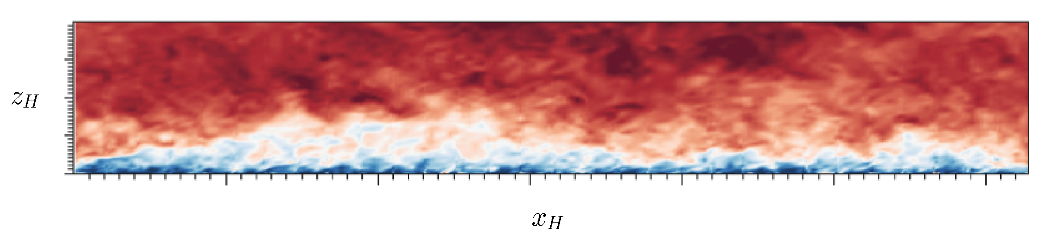
\includegraphics[width = 0.95\linewidth]{Figure/ABL_1.png}
\caption[Snapshot of ABL]{Snapshot of velocity magnitude field of atmospheric boundary layer for Case IX, over the normalized $x-z$ plane. Normalization length scale: BL thickness $H$. Contour colours are based on the magnitude of the velocity, with extreme red: $0.8$ of the maximum, and  extreme blue: $0.05$ of the maximum.}
\end{figure}


\subsection{Effect of Explicit filtering: Variation of $k_c$}
The major comparisons of mean and second order statistics of the atmospheric boundary layer for various degrees of explicit filtering in the near wall model ($k_c = 2, 4, 6$) {have} already {been} discussed in the previous sections. The effect of filtering is not as conspicuous as the shape of $C_s$ (Smagorinsky coefficient) and the discrepancies between different filtering are most prominently seen in the outer layer of the flow, especially in the wake and ``flat-profile" region. Also the outer layer region of $u_{rms}$ shows the worst match with the previous literature for $k_c = 2$. Overall it is observed that results with $k_c = 4, 6$ offer the most reasonable comparison with the literature~\cite{porte1fun}.

{The contribution of the higher bottom wall drag due to turbulence comes from certain region of ``\textit{high-drag patches}" at the wall and not because of an uniform increment in wall shear stress ($\tau_{w}$) compared to its laminar counterpart~\cite{kim1}.}  In the near wall model~(Equation(\ref{stress})), since the information to the wall drag comes from instantaneous horizontal velocities at first grid point from the wall, {low-pass filtering of these variables causes removal of small scale structures while retaining their \textit{large scale} counterpart which still plays a pivotal role in increasing the drag due to turbulence.}  {It is understood, that there is not much differences with filtering $k_c = 2, 4, 6$ since the filtered velocities still contain information of the most important large scale structures which in major may be responsible for the generation of turbulent turbulent drag.} 
It is interesting to note, that for various values of $k_c$ both the energy cascade (1D Energy spectra) at the inner and outer layer of ABL, are monotone invariant of $k_c$ (See Figures~\ref{fig:stat0_lotw2}, $n = 0.5, C_0 = 0.19$). This is further supported by the premultiplied 2D energy spectra in Figures~\ref{fig:2d_spec_diss}, where inconspicuous differences in eddy structures have been observed with variation of $k_c$. {This suggests that the physical mechanism of energy transfer and the scales of motion in the ABL flow are {not strongly affected} by the  ``wall" information.} 

\section{Summary}
The current chapter aims at presenting a higher-order methodology for large eddy simulations of ABL with near wall modelling. Previous literature~\cite{porte1fun,bou1} indicates the limitations of the standard Smagorinsky model as being extremely dissipative in the near wall region preventing the coherent structures to generate \textit{sufficient peaks of Reynolds stresses.}  We have adopted exponentially accurate spectral element discretization in conjunction with standard Smagorinsky model with Mason and Thompson wall damping~\cite{mason} in order to realise the improvement in the atmospheric boundary layer results even with simpler subgrid scale models. We note that due to the fact that spectral element methods are less dissipative {and} dispersive, we need to increase the Smagorinsky coefficient $C_0$ in order to make the second order moments especially \textit{$u_{rms}, \ uw_{rms}$ non-oscillatory in the streamwise direction in near wall region.}. Even increasing $C_0 \ \sim 0.16$ with $n = 2$, we obtain very good match with the second order moments $u_{rms},\ v_{rms}, \ w_{rms}$ with the standard Smagorinsky model results reported in the literature. We also obtained descent match with the scale dependant Smagorinsky model for some statistics {including} in the near wall region for Cases $I-IV$ ($n = 2$). With this model, we obtained excellent linear trends in the kinematic shear stress profile compared to the previous literature results~\cite{calaf,meyers2} and the peak location for all the models (Cases I - X) agree well with the peak of scale-dependant model (See Figure~\ref{fig:peak}). 

However, slight \textit{log-layer mismatch} in the mean velocity trends existed in this model, which can be {effectively} eliminated {yielding} a good match with the log-law, if we use SGS models with $n = \frac{1}{2}$, $C_0 = 0.19$ (cases $VIII-X$). We deducted that lower values of $n$ correspond to a steeper growth of $C_s$ or {increase in} $dC_s/dZ$ which play{s} a crucial role in controlling SGS stresses instead of $C_s$ itself. It was also observed that with $n = \frac{1}{2}$, ``wall drag" $u_{\tau}^2$ increases almost twice as compared to $n = 1,2,3$. It can be seen from Section~\ref{results}, that with $n = \frac{1}{2}$ we have much less dissipation and the results match reasonably well with dynamic Smagorinsky model in the literature.

We also developed approximate shear stress boundary conditions as a tool for the near wall modelling in spectral element methodology. We do not observe any significant difference in results while using different interpolation schemes to connect the outer law velocity fields in the inner shear stress boundary condition. It has been observed, that for a fixed number of grid points, the type of interpolation in the near wall model is not of extreme importance \textit{as long as wall normal extent of the element closest to the wall is not significant.} This is supported by the Figure~\ref{fig:grad2} (spectral and mid-point linear interpolation of NWM) w{h}ere significant difference is not observed in the inner as well as the outer layer. {If we take the outer wall information from grid points further away from the wall the shear stress is noted to decrease as well.~\cite{sag}} 

 Our parametric tests with various $k_c$ and the shape of $C_s$ have revealed a relatively weak influence by the former on the ABL results and yet strong dependence on the latter parameter. We have observed that if we have a sharp growth of $C_s$, such that $dC_s/dz = \kappa$ within $10\%$ of inner layer ($z < 0.1H$), the error due to log-layer mismatch can be eliminated with reasonable amount of success. With cases having high log-layer mismatch, we still observe  over-prediction of peaks of second order statistics despite reasonable match with standard Smagorinsky model.  Also, for the same cases discussed, the near-wall region has a good match with the scale-dependant dynamic models~\cite{porte1fun}. 
 
To summarize, the present work manifests the fact that with higher order discretization methodology, even a relatively simpler subgrid scale model is capable of predicting results which are competent to state-of-art SGS models reported in the literature. The future work would involve developing Smagorinsky models with higher power of gradients (inducing large scale sep{a}ration) which would be more meaningful in higher-order discretization method, and tuning{-}free dynamic and scale dependant subgrid scale model for large-eddy simulation in spectral element framework with high Reynolds number. 